\documentclass[12pt]{article}

% ============================================================
% Packages
% ============================================================

\usepackage[margin=1in]{geometry}
\usepackage{setspace}
\usepackage{graphicx}
\usepackage{booktabs}
\usepackage{placeins}
\usepackage{amsmath}
\usepackage{float}
\usepackage{hyperref}
\usepackage{hyperref}
\usepackage{caption}
\usepackage{subcaption}
\usepackage{array}
\usepackage{xcolor}

% ============================================================
% Formatting
% ============================================================

\onehalfspacing

\hypersetup{
    colorlinks=true,
    linkcolor=blue,
    urlcolor=blue,
    citecolor=blue
}

% ============================================================
% Title Information
% ============================================================

\title{
    \textbf{5291 Final Project Report} \\
    \large Financial Time Series Prediction Using Machine Learning and Numerical Validation Methods
}

\author{
    Baixuan Chen \quad (bc3212) \\
    Purui Niu \quad (pn2433) \\
    Junyang Li \quad (jl7230)
}

\date{
    May 8, 2026 \\[0.5cm]
    \textbf{GitHub Repository:} 
    \href{https://github.com/Trigger-chen/5291_final-project}
    {https://github.com/Trigger-chen/5291\_final-project}
    \\[0.25cm]
    \textbf{Shiny Web Application:} 
    \href{https://baixuanchen5243.shinyapps.io/5291-Final-Project/}
    {https://baixuanchen5243.shinyapps.io/5291-Final-Project/}
}

% ============================================================
% Document Starts
% ============================================================

\begin{document}

\maketitle

\begin{abstract}
This project studies financial time series prediction using multiple asset classes, including precious metals, energy, a currency index, and cryptocurrencies. We first perform data cleaning, preprocessing, exploratory data analysis, and feature engineering. Then, unsupervised learning methods are used to identify latent market patterns, and supervised machine learning models are applied to predict asset returns. Numerical validation methods are further used to reconstruct and evaluate predicted price paths. Finally, an interactive Shiny web application is developed to present the full workflow, allowing users to explore EDA results, model predictions, comparison tables, and numerical validation outputs in a more accessible way.
\end{abstract}

\newpage

\tableofcontents

\newpage

% ============================================================
% 1. Introduction
% ============================================================

\section{Introduction}

Financial markets generate large amounts of time series data that reflect changes in asset prices, risk conditions, and investor behavior. Predicting financial asset returns is challenging because financial time series often contain noise, volatility clustering, nonlinear relationships, and sudden market shocks. Traditional statistical models can capture some patterns in financial returns, but modern machine learning methods provide additional flexibility for modeling complex relationships among multiple assets and engineered market features.

In this project, we study daily financial time series across six representative assets: Gold, Silver, WTI Oil, the U.S. Dollar Index, Bitcoin, and Ethereum. These assets cover different market categories, including precious metals, energy, currency index exposure, and cryptocurrencies. Since these markets may react differently to macroeconomic conditions and investor sentiment, analyzing them together allows us to examine both individual asset behavior and cross-asset relationships.

The main objective of this project is to build a complete machine learning workflow for financial time series prediction. We first collect and clean historical price data, align all assets to common trading days, and transform prices into daily log returns. We then conduct exploratory data analysis to understand price trends, return distributions, volatility patterns, correlations, and extreme return behavior. After that, we construct a feature-engineered dataset that includes lagged returns, rolling statistics, momentum features, volatility ratio features, rolling correlations, drawdown measures, and market regime indicators.

The project also includes unsupervised and supervised learning components. In the unsupervised analysis, principal component analysis, K-Means clustering, and Isolation Forest are used to explore hidden market structures and identify unusual market observations. In the supervised analysis, three machine learning models---Ridge Regression, Random Forest, and Hist Gradient Boosting---are applied to predict next-day returns for each asset. The models are evaluated using time-based train-test splits and standard prediction metrics.

Finally, we apply numerical validation methods to connect return predictions with price path reconstruction. Instead of only evaluating predicted returns, we convert model-predicted returns into predicted prices using one-step-ahead numerical methods such as Euler, Trapezoidal, and RK4-like validation. In addition, we develop an interactive Shiny web application to present the main results, including EDA figures, feature engineering outputs, model comparison tables, prediction plots, and numerical validation results. Overall, this project combines data preprocessing, exploratory analysis, feature engineering, unsupervised learning, supervised machine learning, numerical validation, and web-based presentation into one complete financial time series modeling framework.

% ============================================================
% 2. Data Collection and Preprocessing
% ============================================================

\section{Data Collection and Preprocessing}

\subsection{Data Collection}

The dataset used in this project was collected from Yahoo Finance using the Python package \texttt{yfinance}. We selected six financial assets from different market categories, including precious metals, energy, a currency index, and cryptocurrencies. The selected assets are Gold, Silver, WTI Oil, the U.S. Dollar Index, Bitcoin, and Ethereum. The sample period covers daily observations from January 1, 2016 to March 1, 2026.

\begin{table}[H]
\centering
\caption{Selected Assets and Yahoo Finance Tickers}
\begin{tabular}{ll}
\toprule
\textbf{Asset} & \textbf{Yahoo Finance Ticker} \\
\midrule
Gold & GC=F \\
Silver & SI=F \\
WTI Oil & CL=F \\
U.S. Dollar Index & DX-Y.NYB \\
Bitcoin & BTC-USD \\
Ethereum & ETH-USD \\
\bottomrule
\end{tabular}
\end{table}

After downloading the raw data, the dataset contained 3,713 daily rows and 36 columns. Since Yahoo Finance returns multiple price fields such as Open, High, Low, Close, Adjusted Close, and Volume, we extracted the Adjusted Close price when available. Adjusted Close was preferred because it provides a consistent price series after accounting for price adjustments. The ticker columns were then renamed into readable asset names.

\subsection{Data Quality Check and Cleaning}

Before constructing return series, we performed a data quality check on missing values and invalid prices. The original data contained missing observations because traditional financial assets and cryptocurrencies do not always share the same trading calendar. For example, cryptocurrencies trade every day, while commodity futures and the U.S. Dollar Index follow market trading days.

\begin{table}[H]
\centering
\caption{Missing Values Before Cleaning}
\begin{tabular}{lr}
\toprule
\textbf{Asset} & \textbf{Missing Values} \\
\midrule
Gold & 1161 \\
Silver & 1161 \\
WTI Oil & 1160 \\
U.S. Dollar Index & 1159 \\
Bitcoin & 0 \\
Ethereum & 678 \\
\bottomrule
\end{tabular}
\end{table}

We also checked whether any asset had non-positive prices. This step is necessary because log returns require strictly positive prices. The data quality check found one non-positive observation in WTI Oil, while the other assets had no non-positive prices.

\begin{table}[H]
\centering
\caption{Non-Positive Prices Before Cleaning}
\begin{tabular}{lr}
\toprule
\textbf{Asset} & \textbf{Non-Positive Prices} \\
\midrule
Gold & 0 \\
Silver & 0 \\
WTI Oil & 1 \\
U.S. Dollar Index & 0 \\
Bitcoin & 0 \\
Ethereum & 0 \\
\bottomrule
\end{tabular}
\end{table}

To clean the price data, all non-positive prices were replaced with missing values. Then, we kept only the dates where all six assets had valid prices. This produced an aligned common-trading-day dataset with 2,084 observations and 6 asset columns.

\begin{table}[H]
\centering
\caption{Cleaned Price Dataset Summary}
\begin{tabular}{ll}
\toprule
\textbf{Item} & \textbf{Result} \\
\midrule
Date range before cleaning & 2016-01-01 to 2026-03-01 \\
Cleaned price data shape & 2084 rows $\times$ 6 columns \\
Missing values after cleaning & 0 \\
Number of assets & 6 \\
\bottomrule
\end{tabular}
\end{table}

\subsection{Log Return Transformation}

Financial price levels are usually non-stationary, so we transformed the cleaned price series into daily log returns. Log returns are commonly used in financial modeling because they are additive over time and more suitable for statistical and machine learning models than raw prices.

For each asset, the daily log return was computed as

\begin{equation}
r_t = \log(P_t) - \log(P_{t-1}),
\end{equation}

where $P_t$ is the asset price at time $t$, and $r_t$ is the daily log return. After differencing, the return dataset contained 2,083 observations and 6 columns, with no missing values.

\begin{table}[H]
\centering
\caption{Log Return Dataset Summary}
\begin{tabular}{ll}
\toprule
\textbf{Item} & \textbf{Result} \\
\midrule
Return data shape & 2083 rows $\times$ 6 columns \\
Missing values in returns & 0 \\
Return frequency & Daily \\
Return type & Log return \\
\bottomrule
\end{tabular}
\end{table}

\subsection{Basic Machine Learning Feature Construction}

After computing daily log returns, we created a supervised machine learning dataset. The initial target variable was defined as the next-day Bitcoin return. The explanatory variables include lagged returns, rolling mean returns, and rolling volatility features for all six assets.

The target variable is defined as

\begin{equation}
y_t = r^{Bitcoin}_{t+1},
\end{equation}

where $r^{Bitcoin}_{t+1}$ is the next-day Bitcoin log return. The main feature groups are summarized below.

\begin{table}[H]
\centering
\caption{Basic Machine Learning Feature Groups}
\begin{tabular}{ll}
\toprule
\textbf{Feature Group} & \textbf{Description} \\
\midrule
Lagged returns & Previous 1, 2, 3, and 5-day returns for each asset \\
Rolling mean returns & 5, 10, and 20-day rolling average returns \\
Rolling volatility & 5, 10, and 20-day rolling standard deviation of returns \\
Target variable & Next-day Bitcoin log return \\
\bottomrule
\end{tabular}
\end{table}

The resulting machine learning dataset contained 2,063 observations and 61 columns. Among these columns, 60 were predictor variables and 1 was the target variable.

\begin{table}[H]
\centering
\caption{Initial Machine Learning Dataset Summary}
\begin{tabular}{ll}
\toprule
\textbf{Item} & \textbf{Result} \\
\midrule
Machine learning dataset shape & 2063 rows $\times$ 61 columns \\
Feature matrix shape & 2063 rows $\times$ 60 columns \\
Target vector shape & 2063 rows \\
Target variable & Bitcoin next-day log return \\
\bottomrule
\end{tabular}
\end{table}

\subsection{Time-Based Train-Test Split and Feature Scaling}

Because the data are time series observations, we used a chronological train-test split instead of random shuffling. The first 70\% of the observations were used as the training set, and the remaining 30\% were used as the testing set. This prevents future information from leaking into the training process.

\begin{table}[H]
\centering
\caption{Time-Based Train-Test Split}
\begin{tabular}{lll}
\toprule
\textbf{Dataset} & \textbf{Date Range} & \textbf{Shape} \\
\midrule
Training set & 2017-12-08 to 2023-09-08 & 1444 rows $\times$ 60 features \\
Testing set & 2023-09-11 to 2026-02-26 & 619 rows $\times$ 60 features \\
\bottomrule
\end{tabular}
\end{table}

Feature standardization was then applied using \texttt{StandardScaler}. To avoid data leakage, the scaler was fitted only on the training feature matrix and then applied to the testing feature matrix. After scaling, both the training and testing feature matrices contained no missing or infinite values.

\begin{table}[H]
\centering
\caption{Final Preprocessed Dataset Check}
\begin{tabular}{ll}
\toprule
\textbf{Item} & \textbf{Result} \\
\midrule
NaN values in scaled training features & 0 \\
NaN values in scaled testing features & 0 \\
Infinite values in scaled training features & 0 \\
Infinite values in scaled testing features & 0 \\
Final scaled training feature shape & 1444 rows $\times$ 60 columns \\
Final scaled testing feature shape & 619 rows $\times$ 60 columns \\
\bottomrule
\end{tabular}
\end{table}

The cleaned and preprocessed datasets were saved as CSV files for later exploratory analysis, feature engineering, unsupervised learning, and supervised machine learning modeling. These files include cleaned asset prices, daily log returns, the initial machine learning feature table, scaled training and testing features, and corresponding target vectors.

% ============================================================
% 3. Exploratory Data Analysis
% ============================================================

\section{Exploratory Data Analysis}

After data cleaning and preprocessing, we conducted exploratory data analysis to understand the behavior of the six financial assets. The EDA focuses on price trends, return fluctuations, volatility patterns, correlation structure, and risk-return characteristics. These analyses help motivate the later feature engineering and machine learning modeling steps.

\subsection{Price Trend Analysis}

We first compared the price movements of the six assets over the full sample period. Since the assets have very different price scales, we used normalized prices with the initial value set to 100. This allows us to compare relative growth patterns across assets.

\begin{figure}[!htbp]
    \centering
    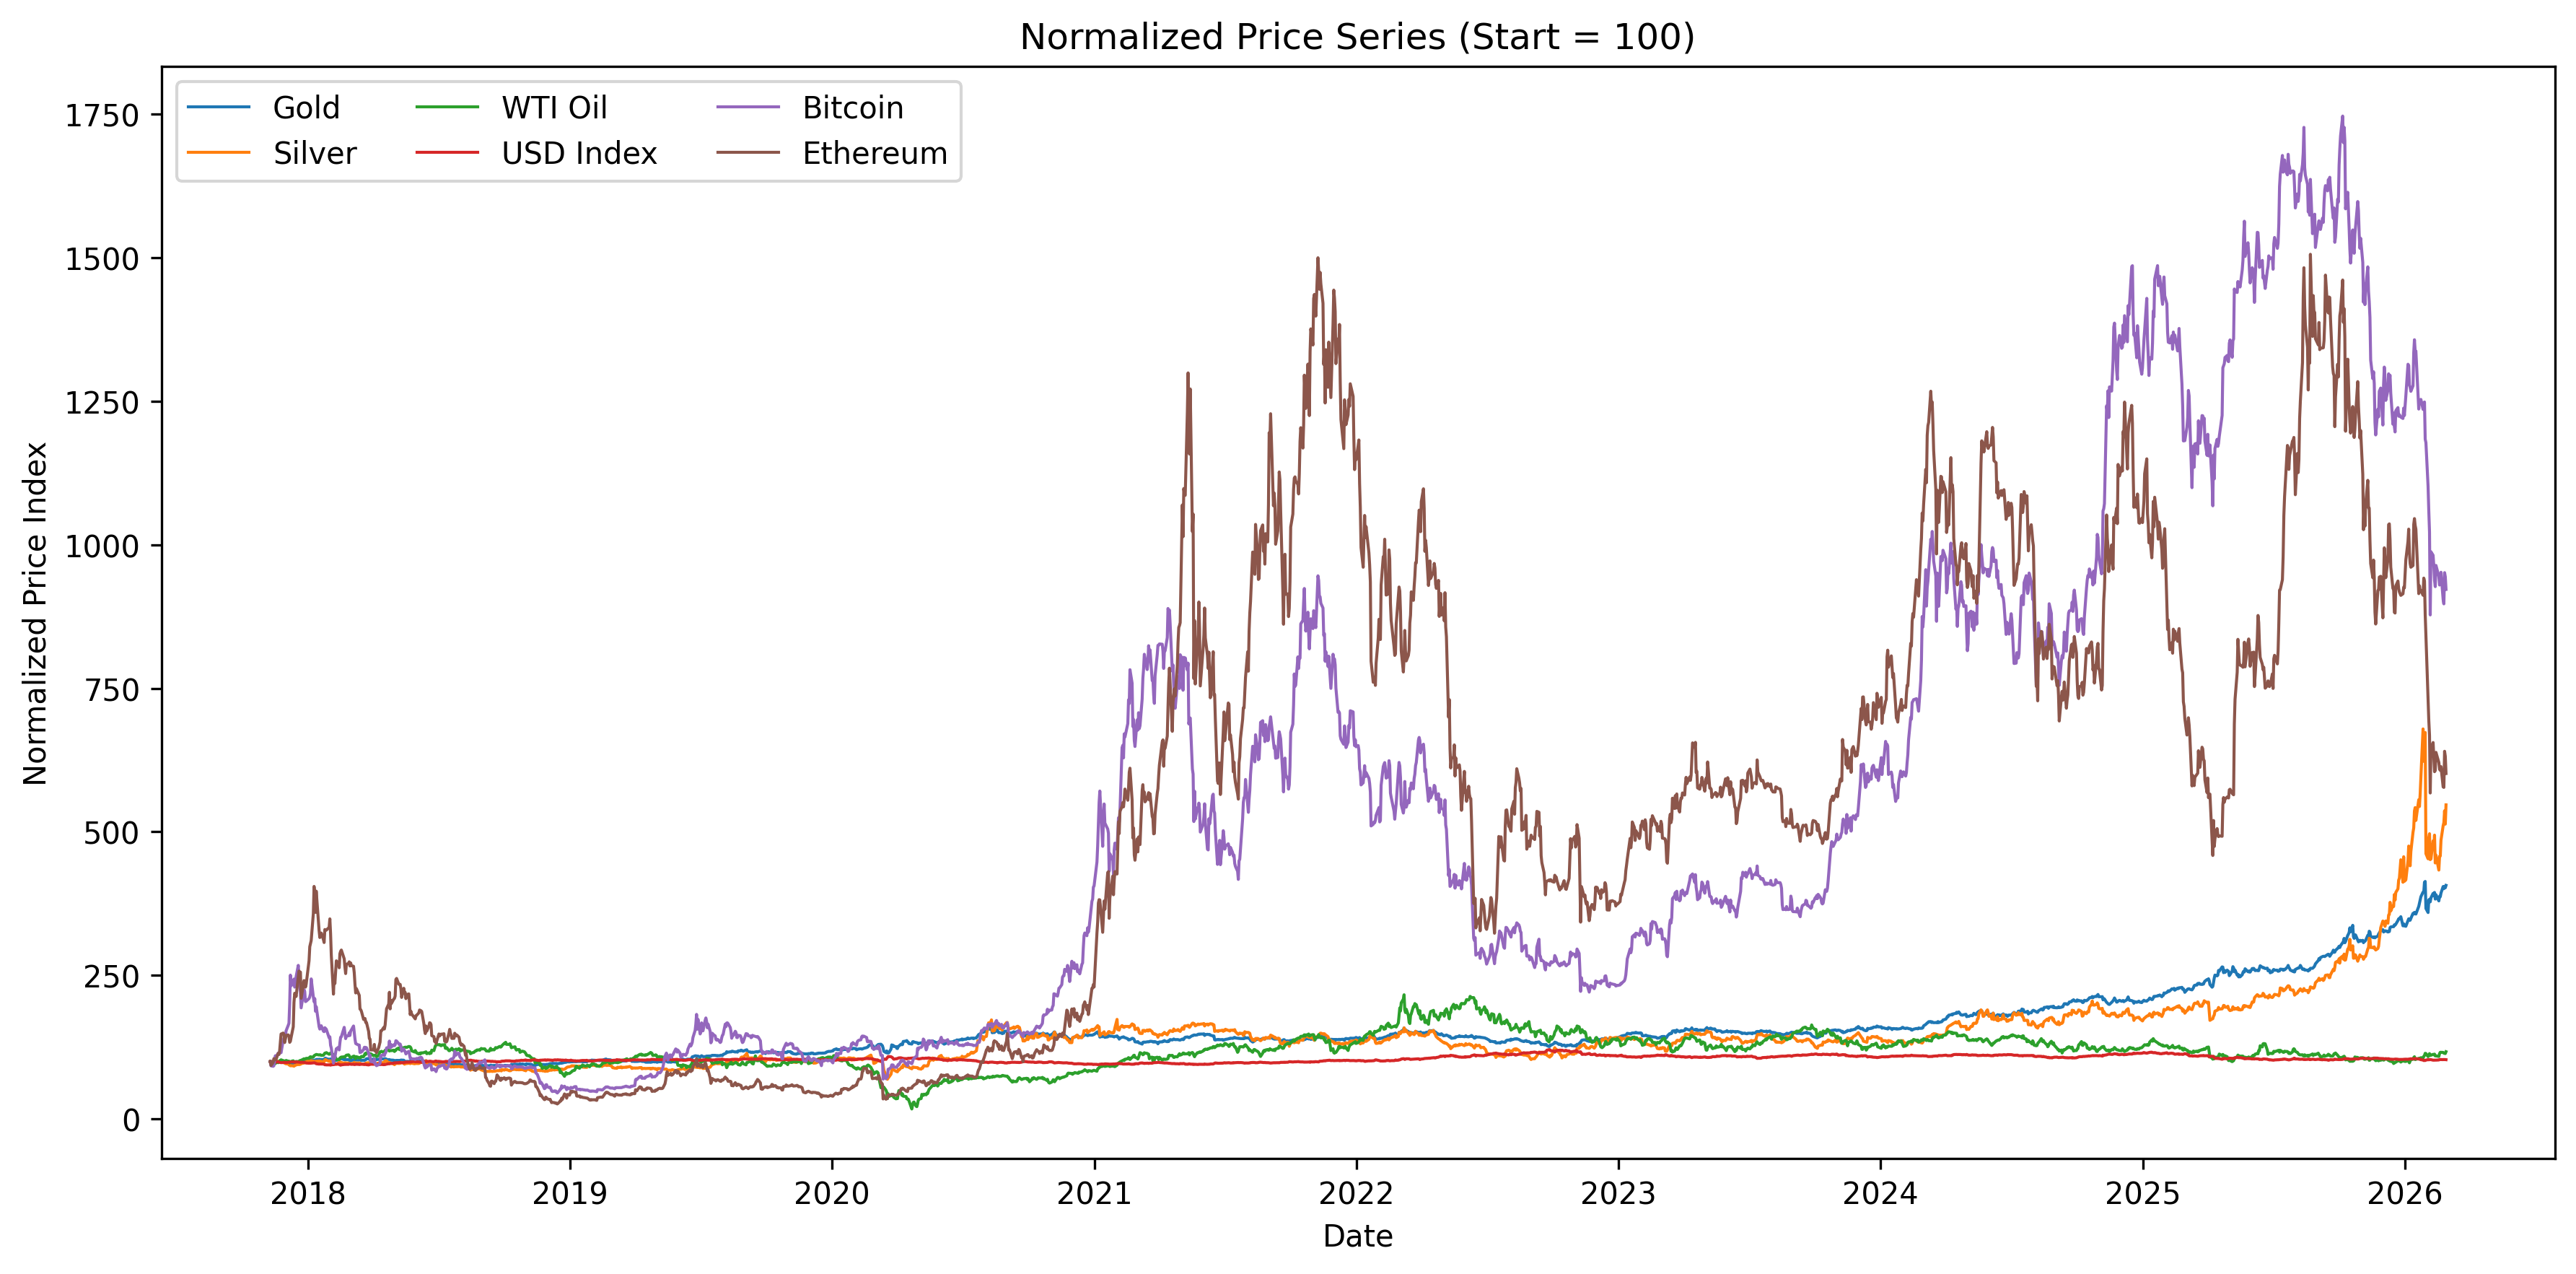
\includegraphics[width=0.72\textwidth]{EDA_plot/normalized_price_series.png}
    \caption{Normalized Price Series of Six Assets}
    \label{fig:normalized_price}
\end{figure}

The normalized price plot shows that cryptocurrencies, especially Bitcoin and Ethereum, experienced much larger growth and stronger fluctuations than traditional assets. Gold and Silver show more moderate upward trends, while WTI Oil and the U.S. Dollar Index display different cyclical patterns. This suggests that the assets have different risk and return profiles.

\FloatBarrier


\subsection{Return Pattern Analysis}

Next, we examined daily log returns. Compared with price levels, log returns fluctuate around zero and are more suitable for machine learning models. The return time series also shows volatility clustering, meaning that large changes tend to occur in groups rather than independently over time.

\begin{figure}[!htbp]
    \centering
    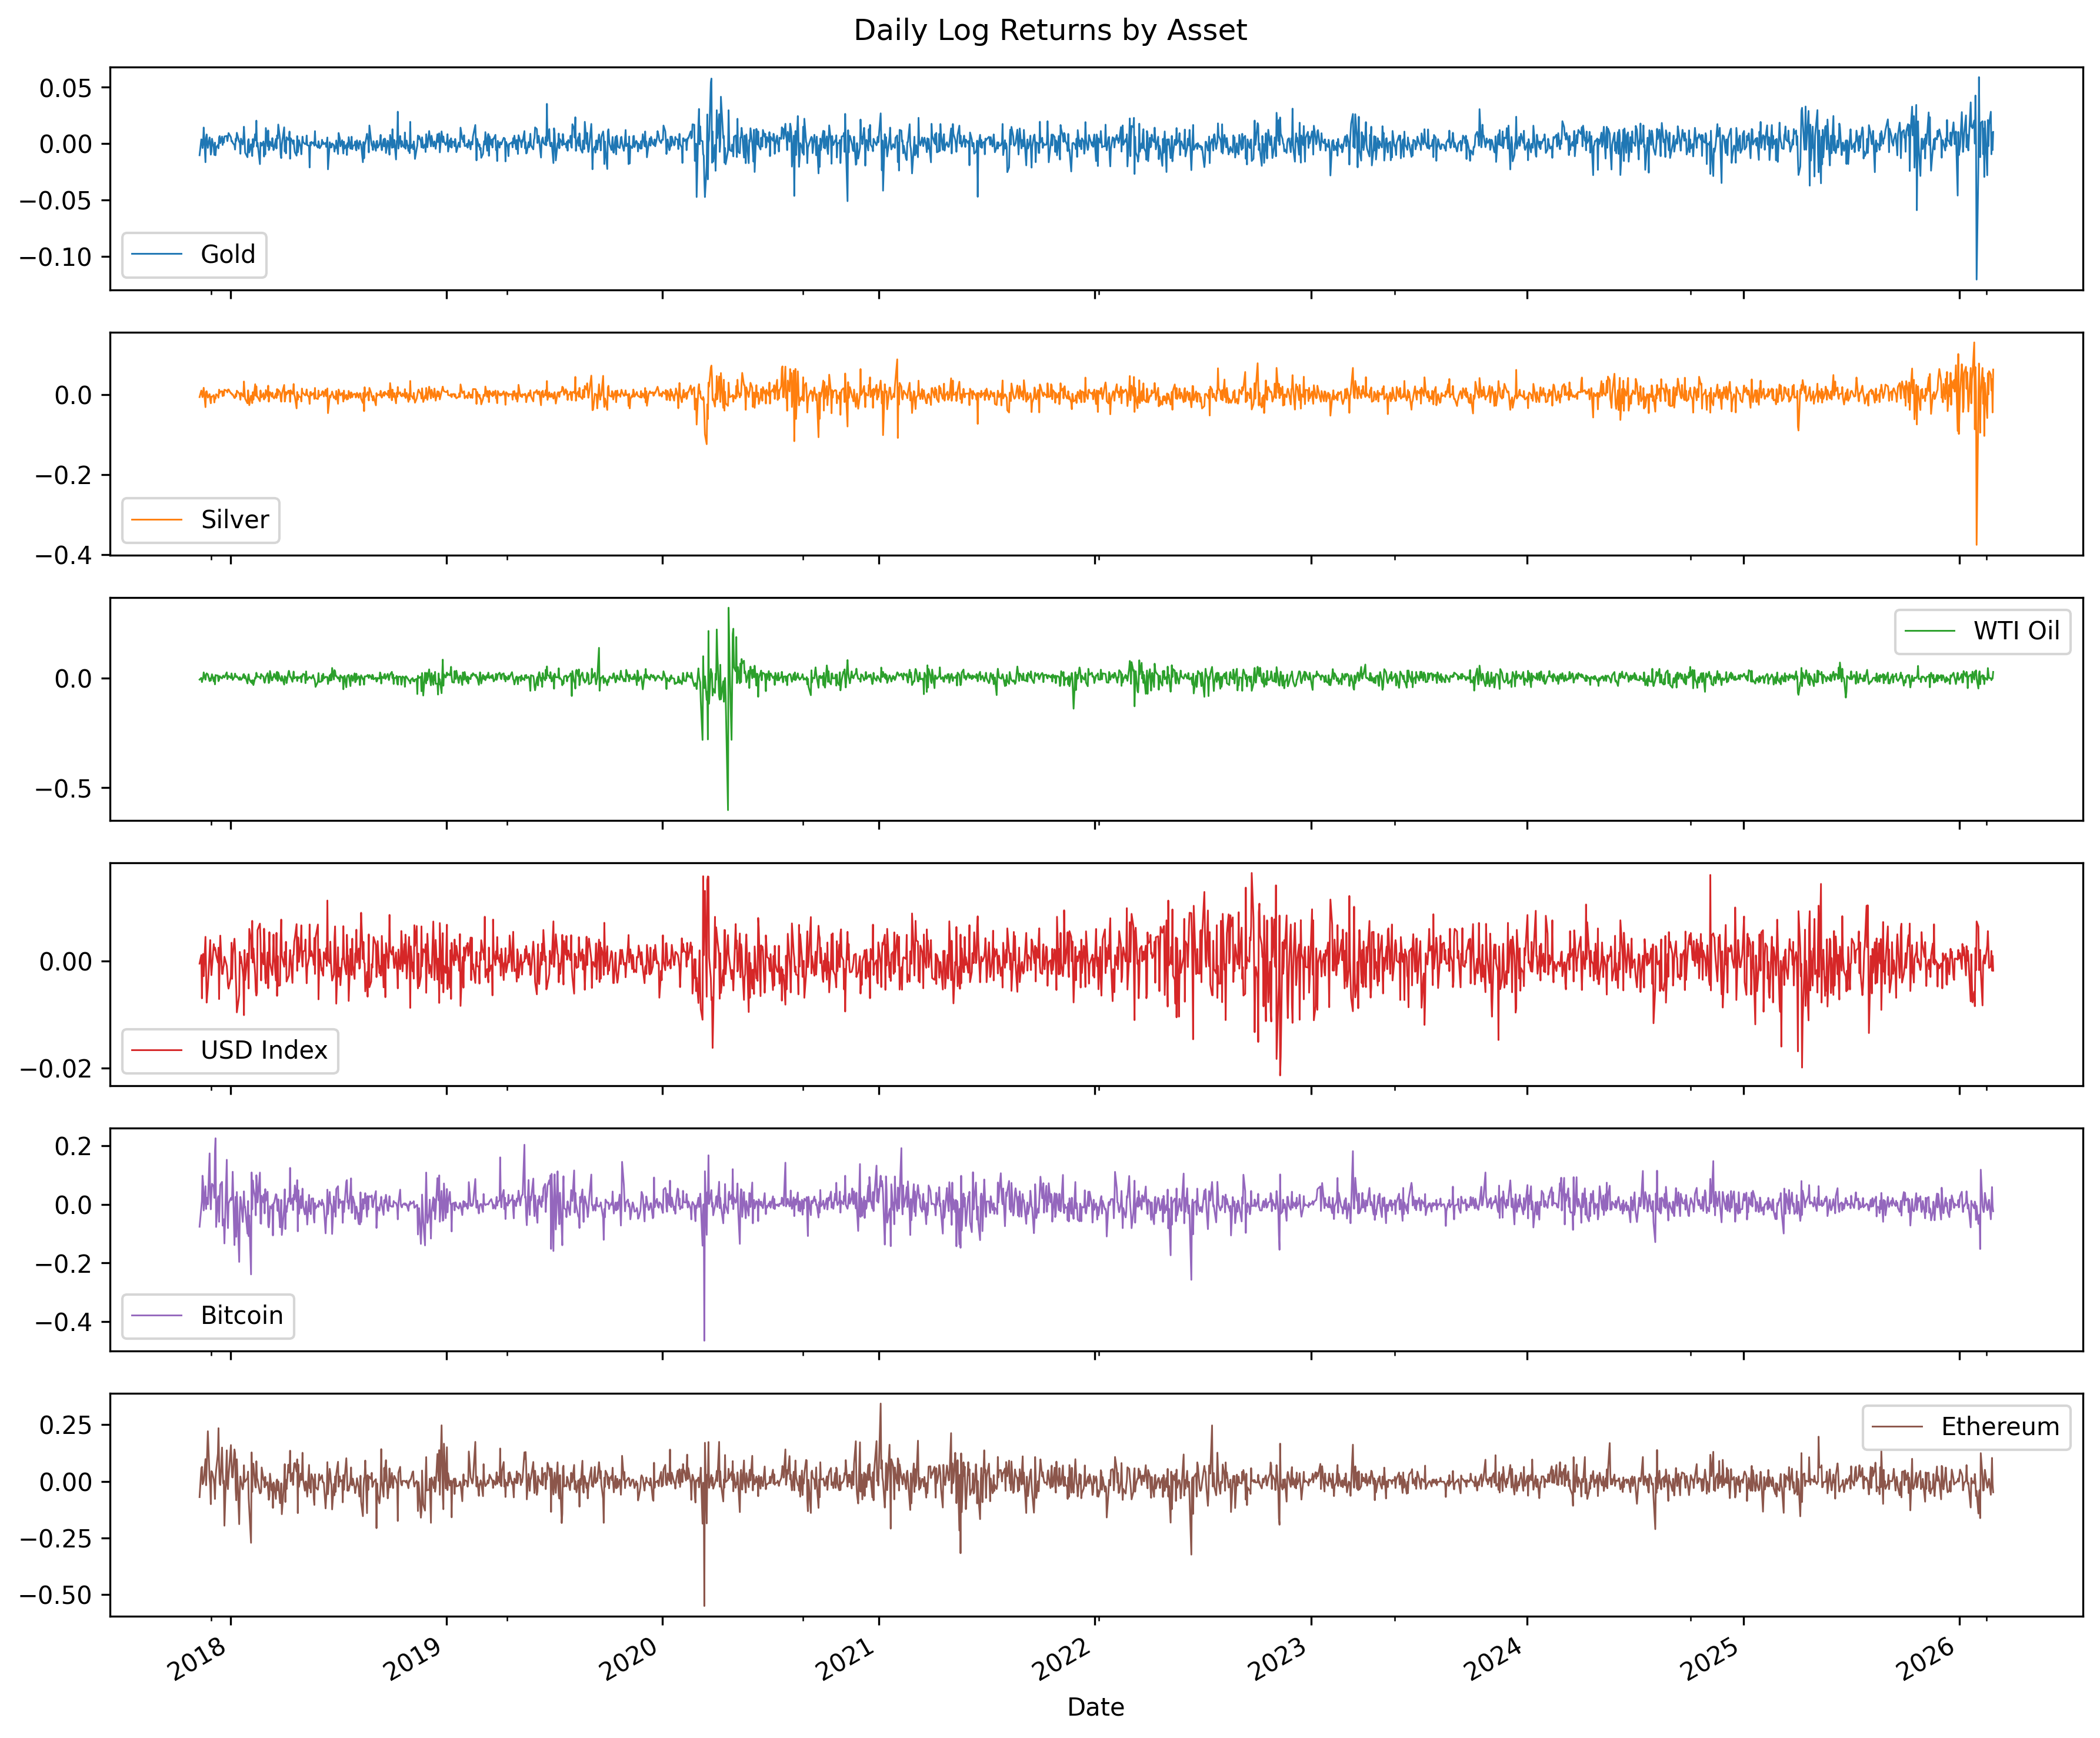
\includegraphics[width=0.68\textwidth]{EDA_plot/daily_log_returns.png}
    \caption{Daily Log Returns of Six Assets}
    \label{fig:daily_log_returns}
\end{figure}

The return plot indicates that cryptocurrencies have larger daily return fluctuations than metals, oil, and the currency index. Some periods contain unusually large positive or negative returns, which motivates the construction of volatility and extreme-return features in the feature engineering stage.

\FloatBarrier


\subsection{Volatility Analysis}

To better understand time-varying risk, we computed rolling volatility using daily log returns. Rolling volatility captures how market uncertainty changes over time. We also annualized the rolling volatility to make the magnitude easier to interpret.

\begin{figure}[!htbp]
    \centering
    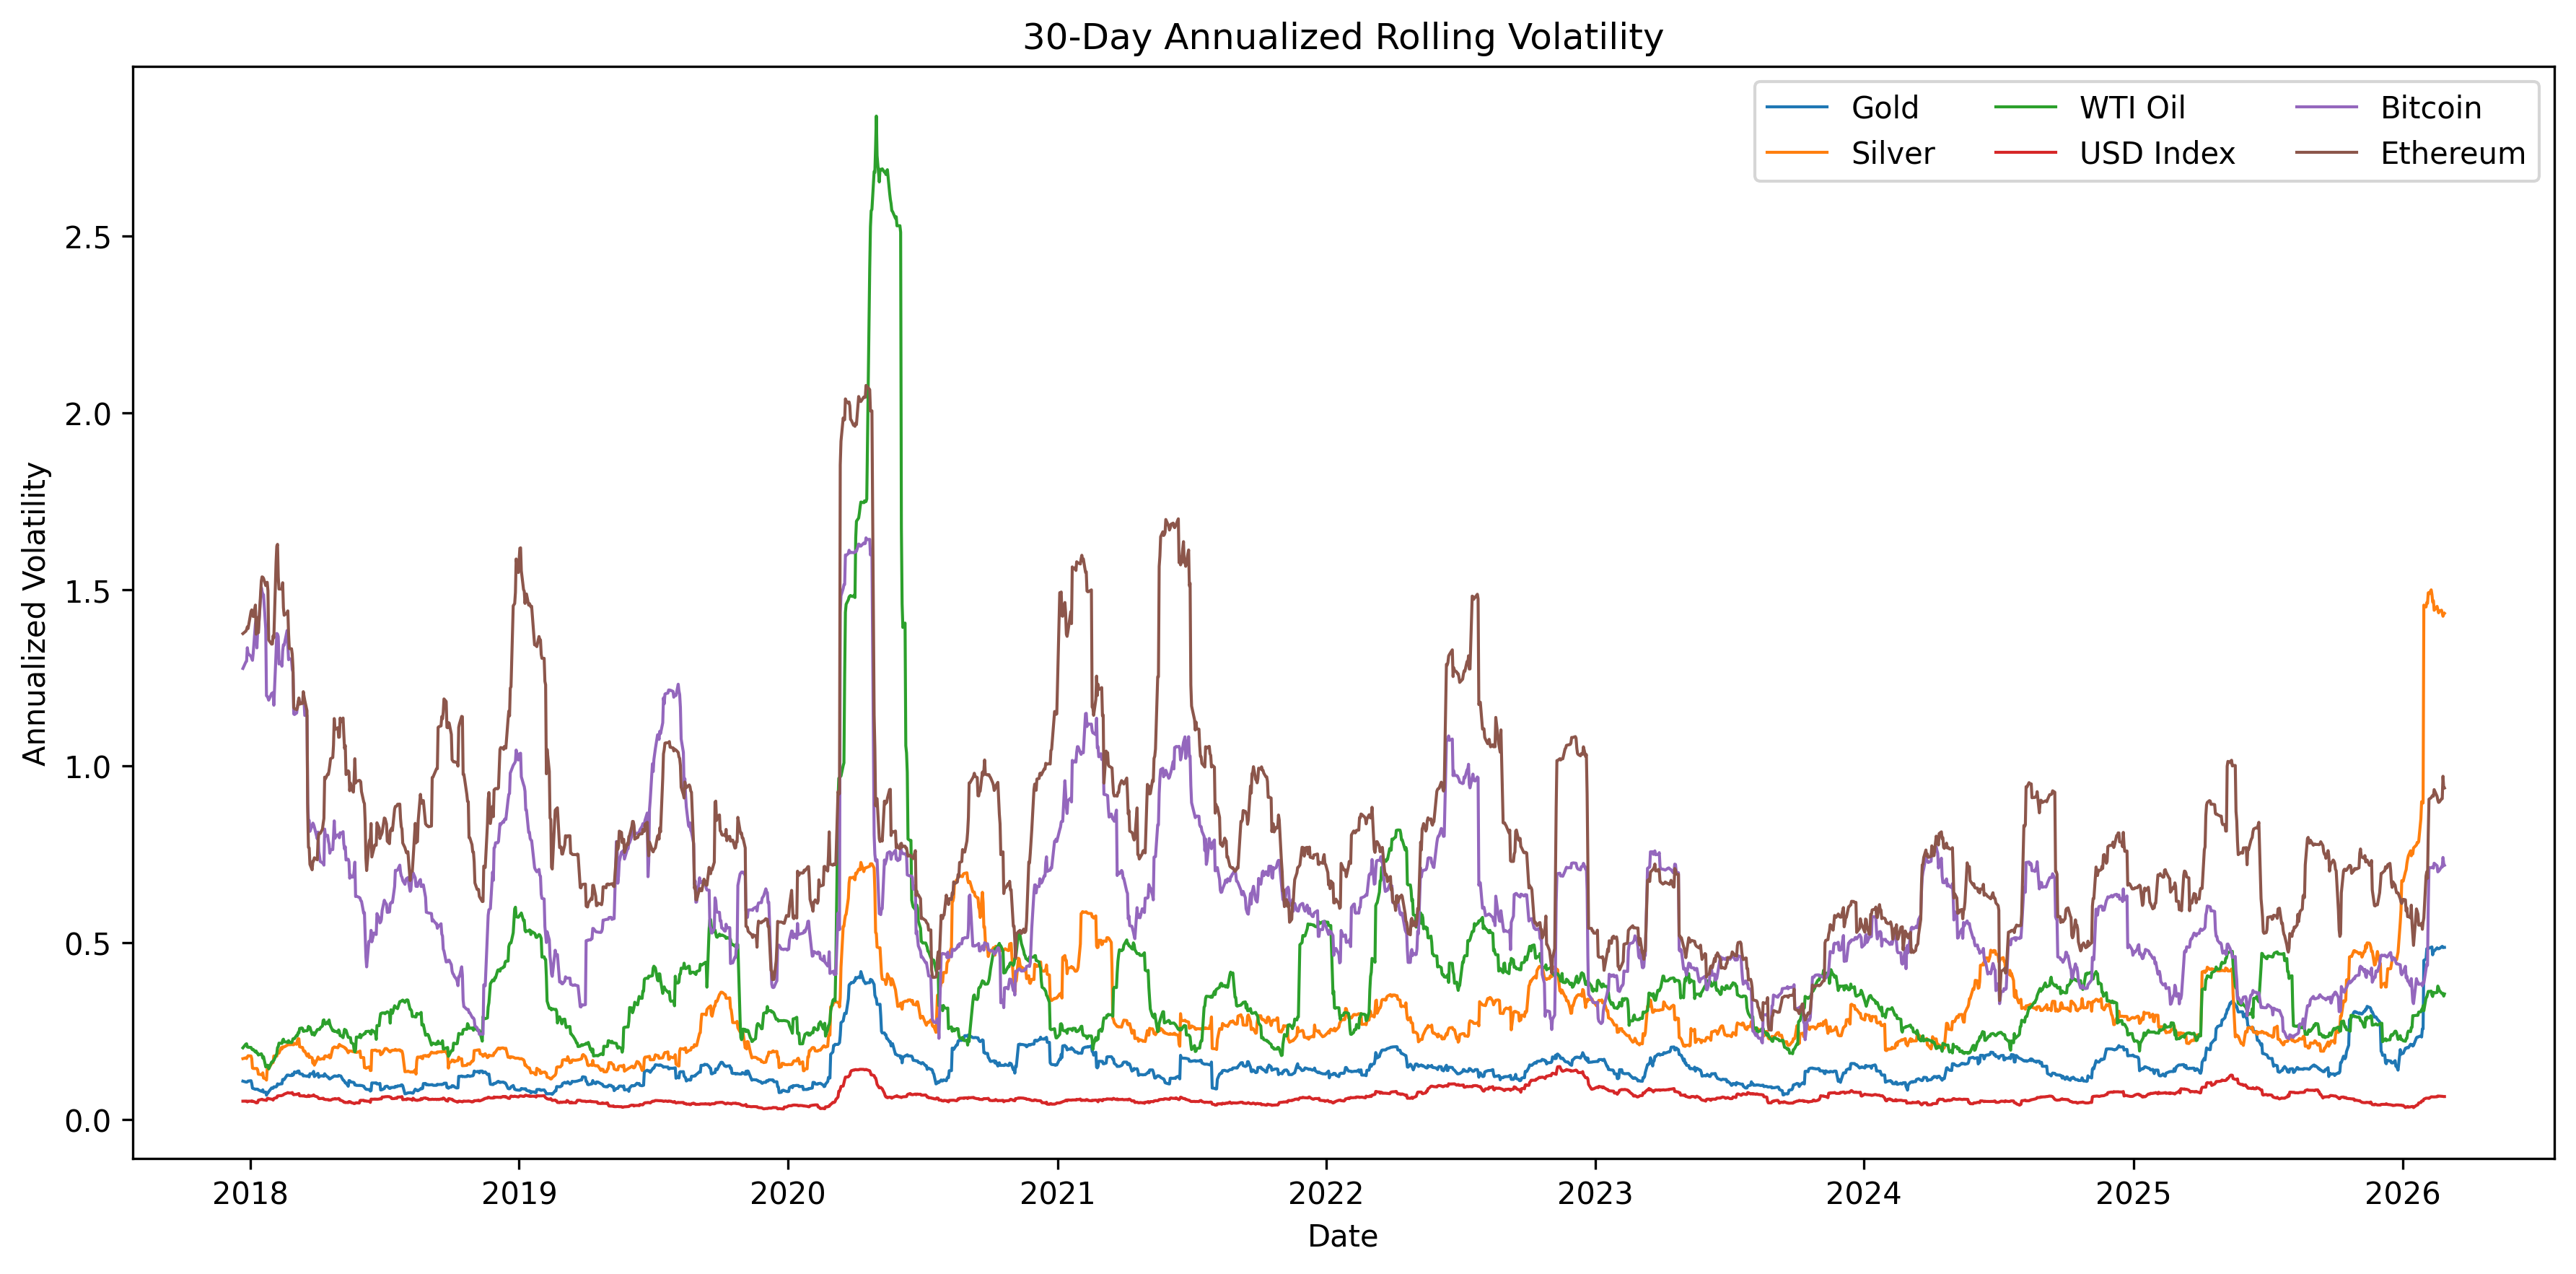
\includegraphics[width=0.72\textwidth]{EDA_plot/rolling_volatility.png}
    \caption{30-Day Annualized Rolling Volatility}
    \label{fig:rolling_volatility}
\end{figure}

The volatility plot confirms that financial risk is not constant over time. Bitcoin, Ethereum, and WTI Oil show much stronger volatility spikes than the other assets. This supports the use of rolling volatility, volatility ratio, and volatility regime indicators as predictive features.

\FloatBarrier


\subsection{Correlation Analysis}

We also examined the correlation matrix of daily log returns to understand cross-asset relationships. Correlation analysis is important because the prediction models use information from all assets to forecast future returns.

\begin{figure}[!htbp]
    \centering
    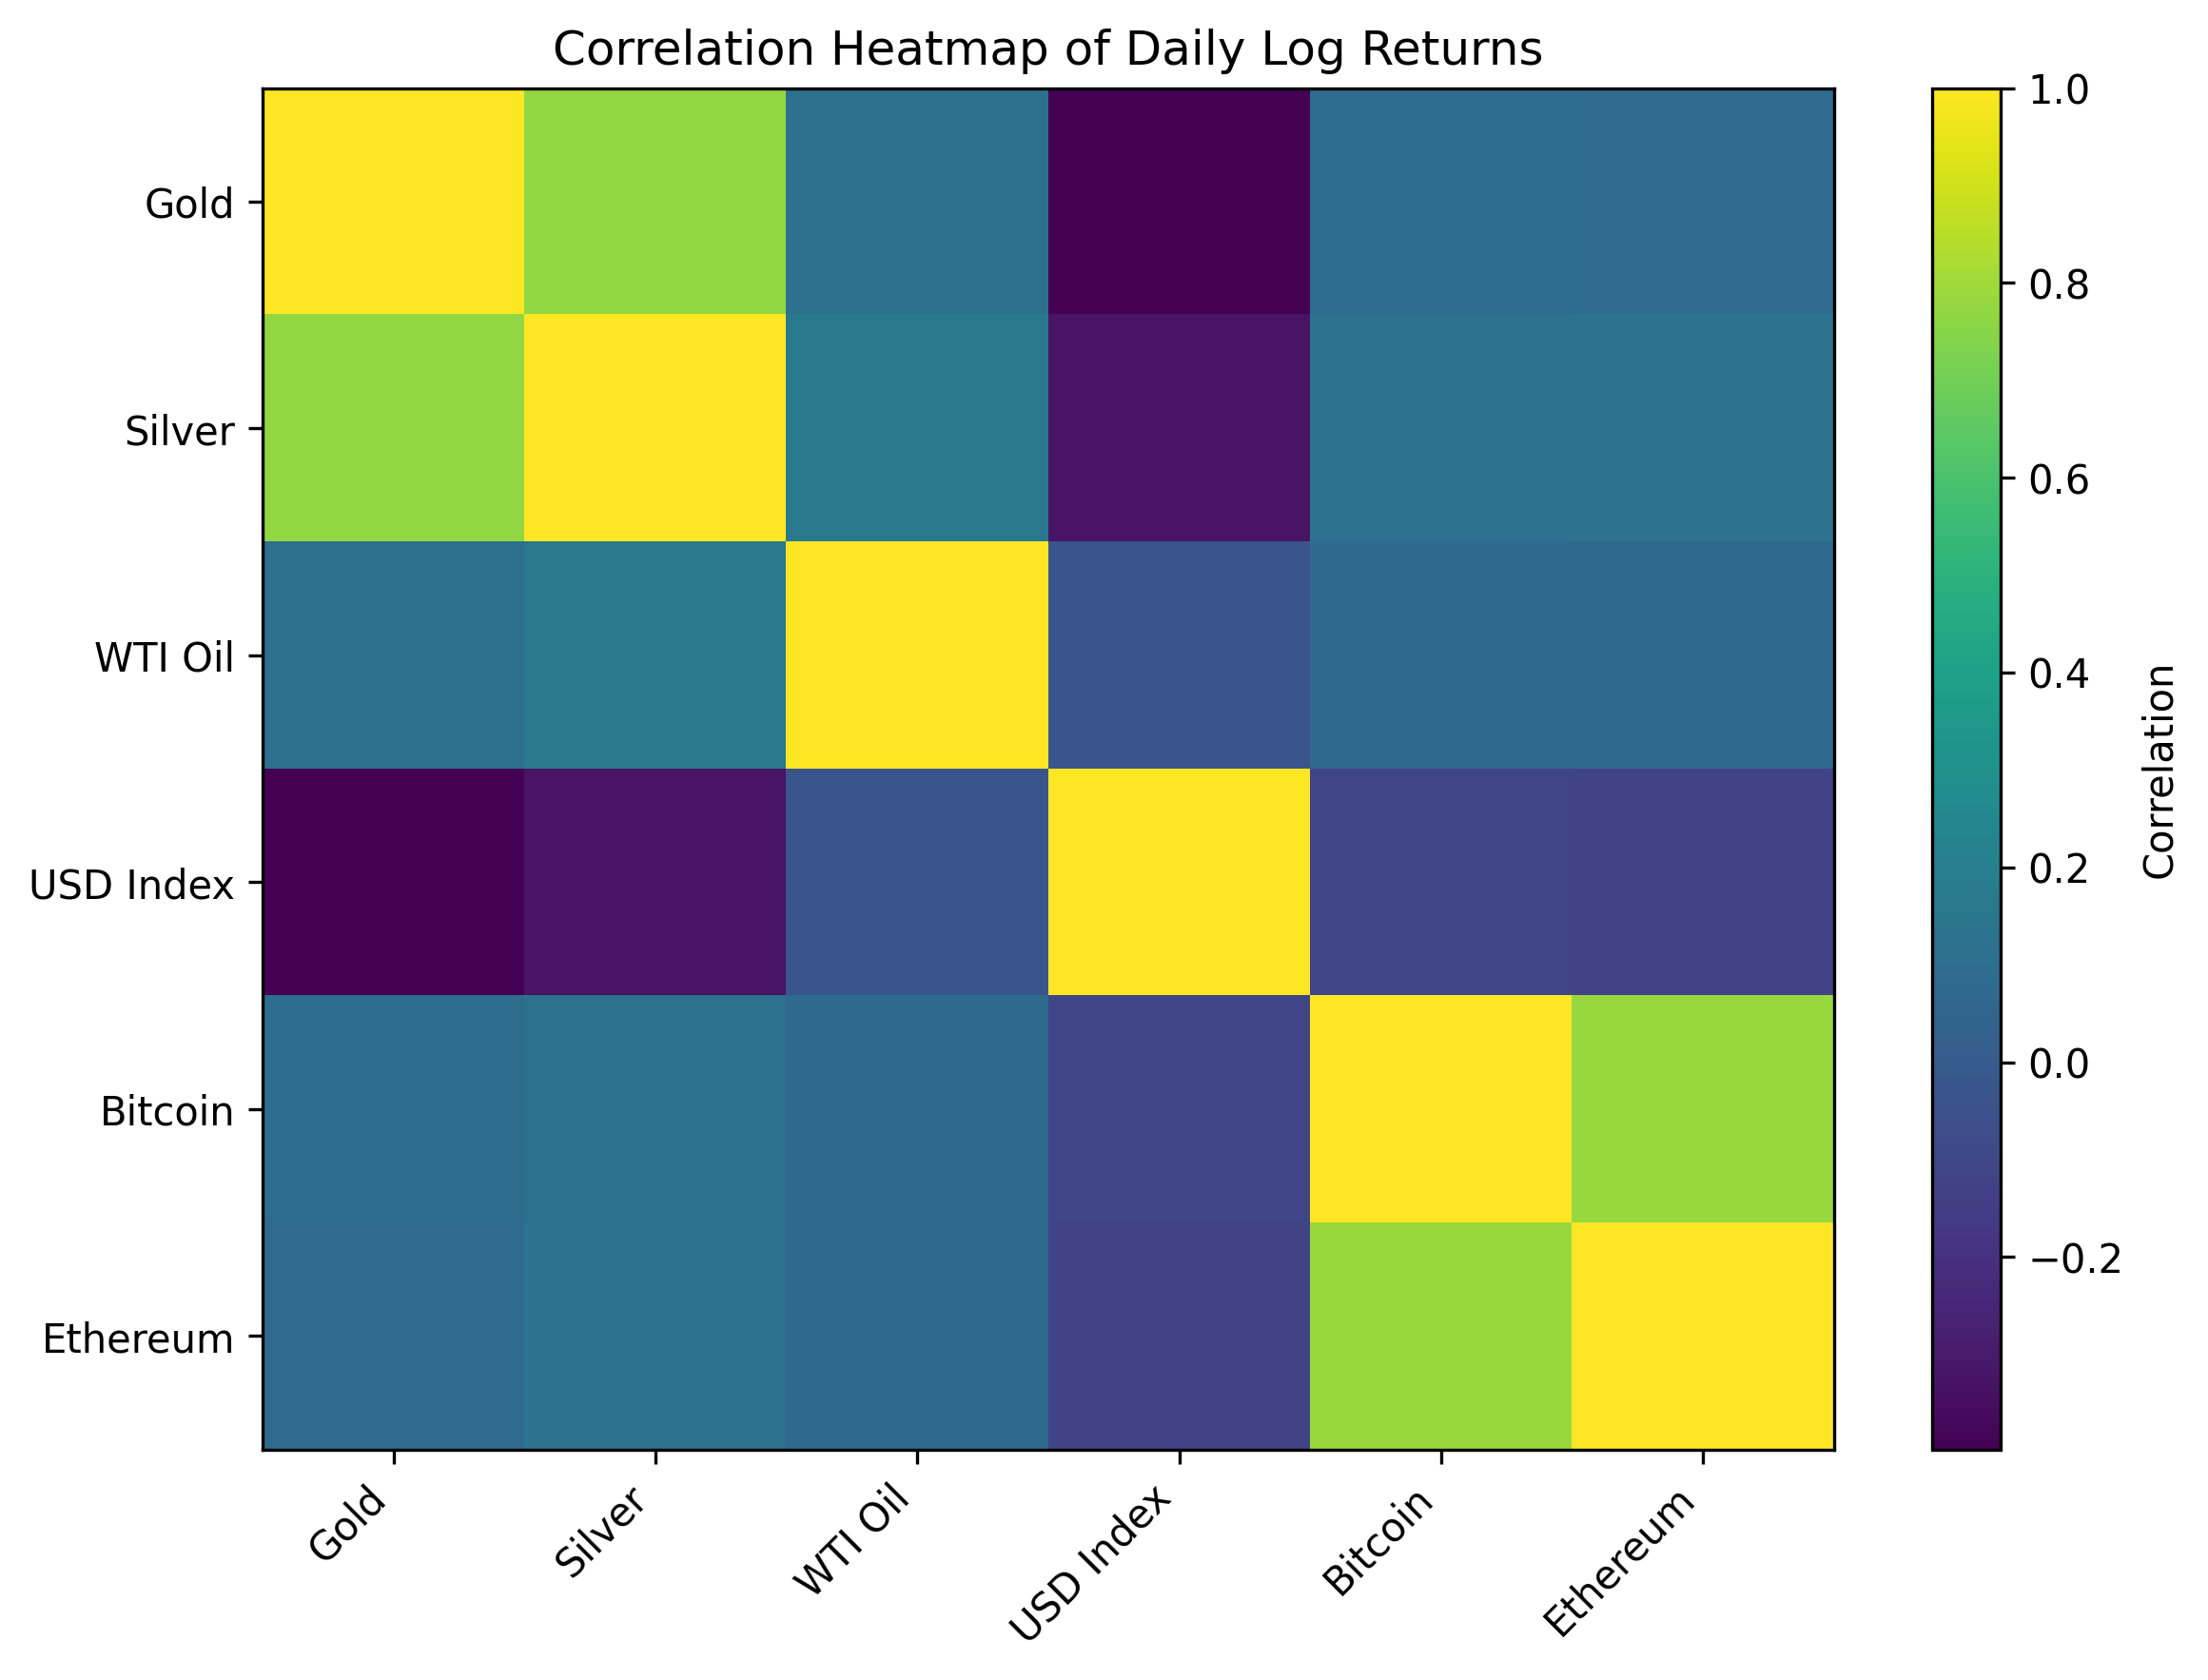
\includegraphics[width=0.56\textwidth]{EDA_plot/correlation_heatmap.png}
    \caption{Correlation Heatmap of Daily Log Returns}
    \label{fig:correlation_heatmap}
\end{figure}

The correlation heatmap shows that some assets move together more closely than others. For example, assets within similar market categories may show stronger correlation, while assets from different categories may provide different information. Since these relationships may change over time, rolling correlation features are later added to the machine learning dataset.

\FloatBarrier


\subsection{Risk-Return Summary}

Finally, we summarized each asset's annualized mean return, annualized volatility, skewness, and excess kurtosis. This provides a compact comparison of expected return, risk level, and tail behavior across assets. In general, cryptocurrencies have higher volatility and more extreme return behavior, while Gold, Silver, and the U.S. Dollar Index are relatively more stable.

\begin{figure}[!htbp]
    \centering
    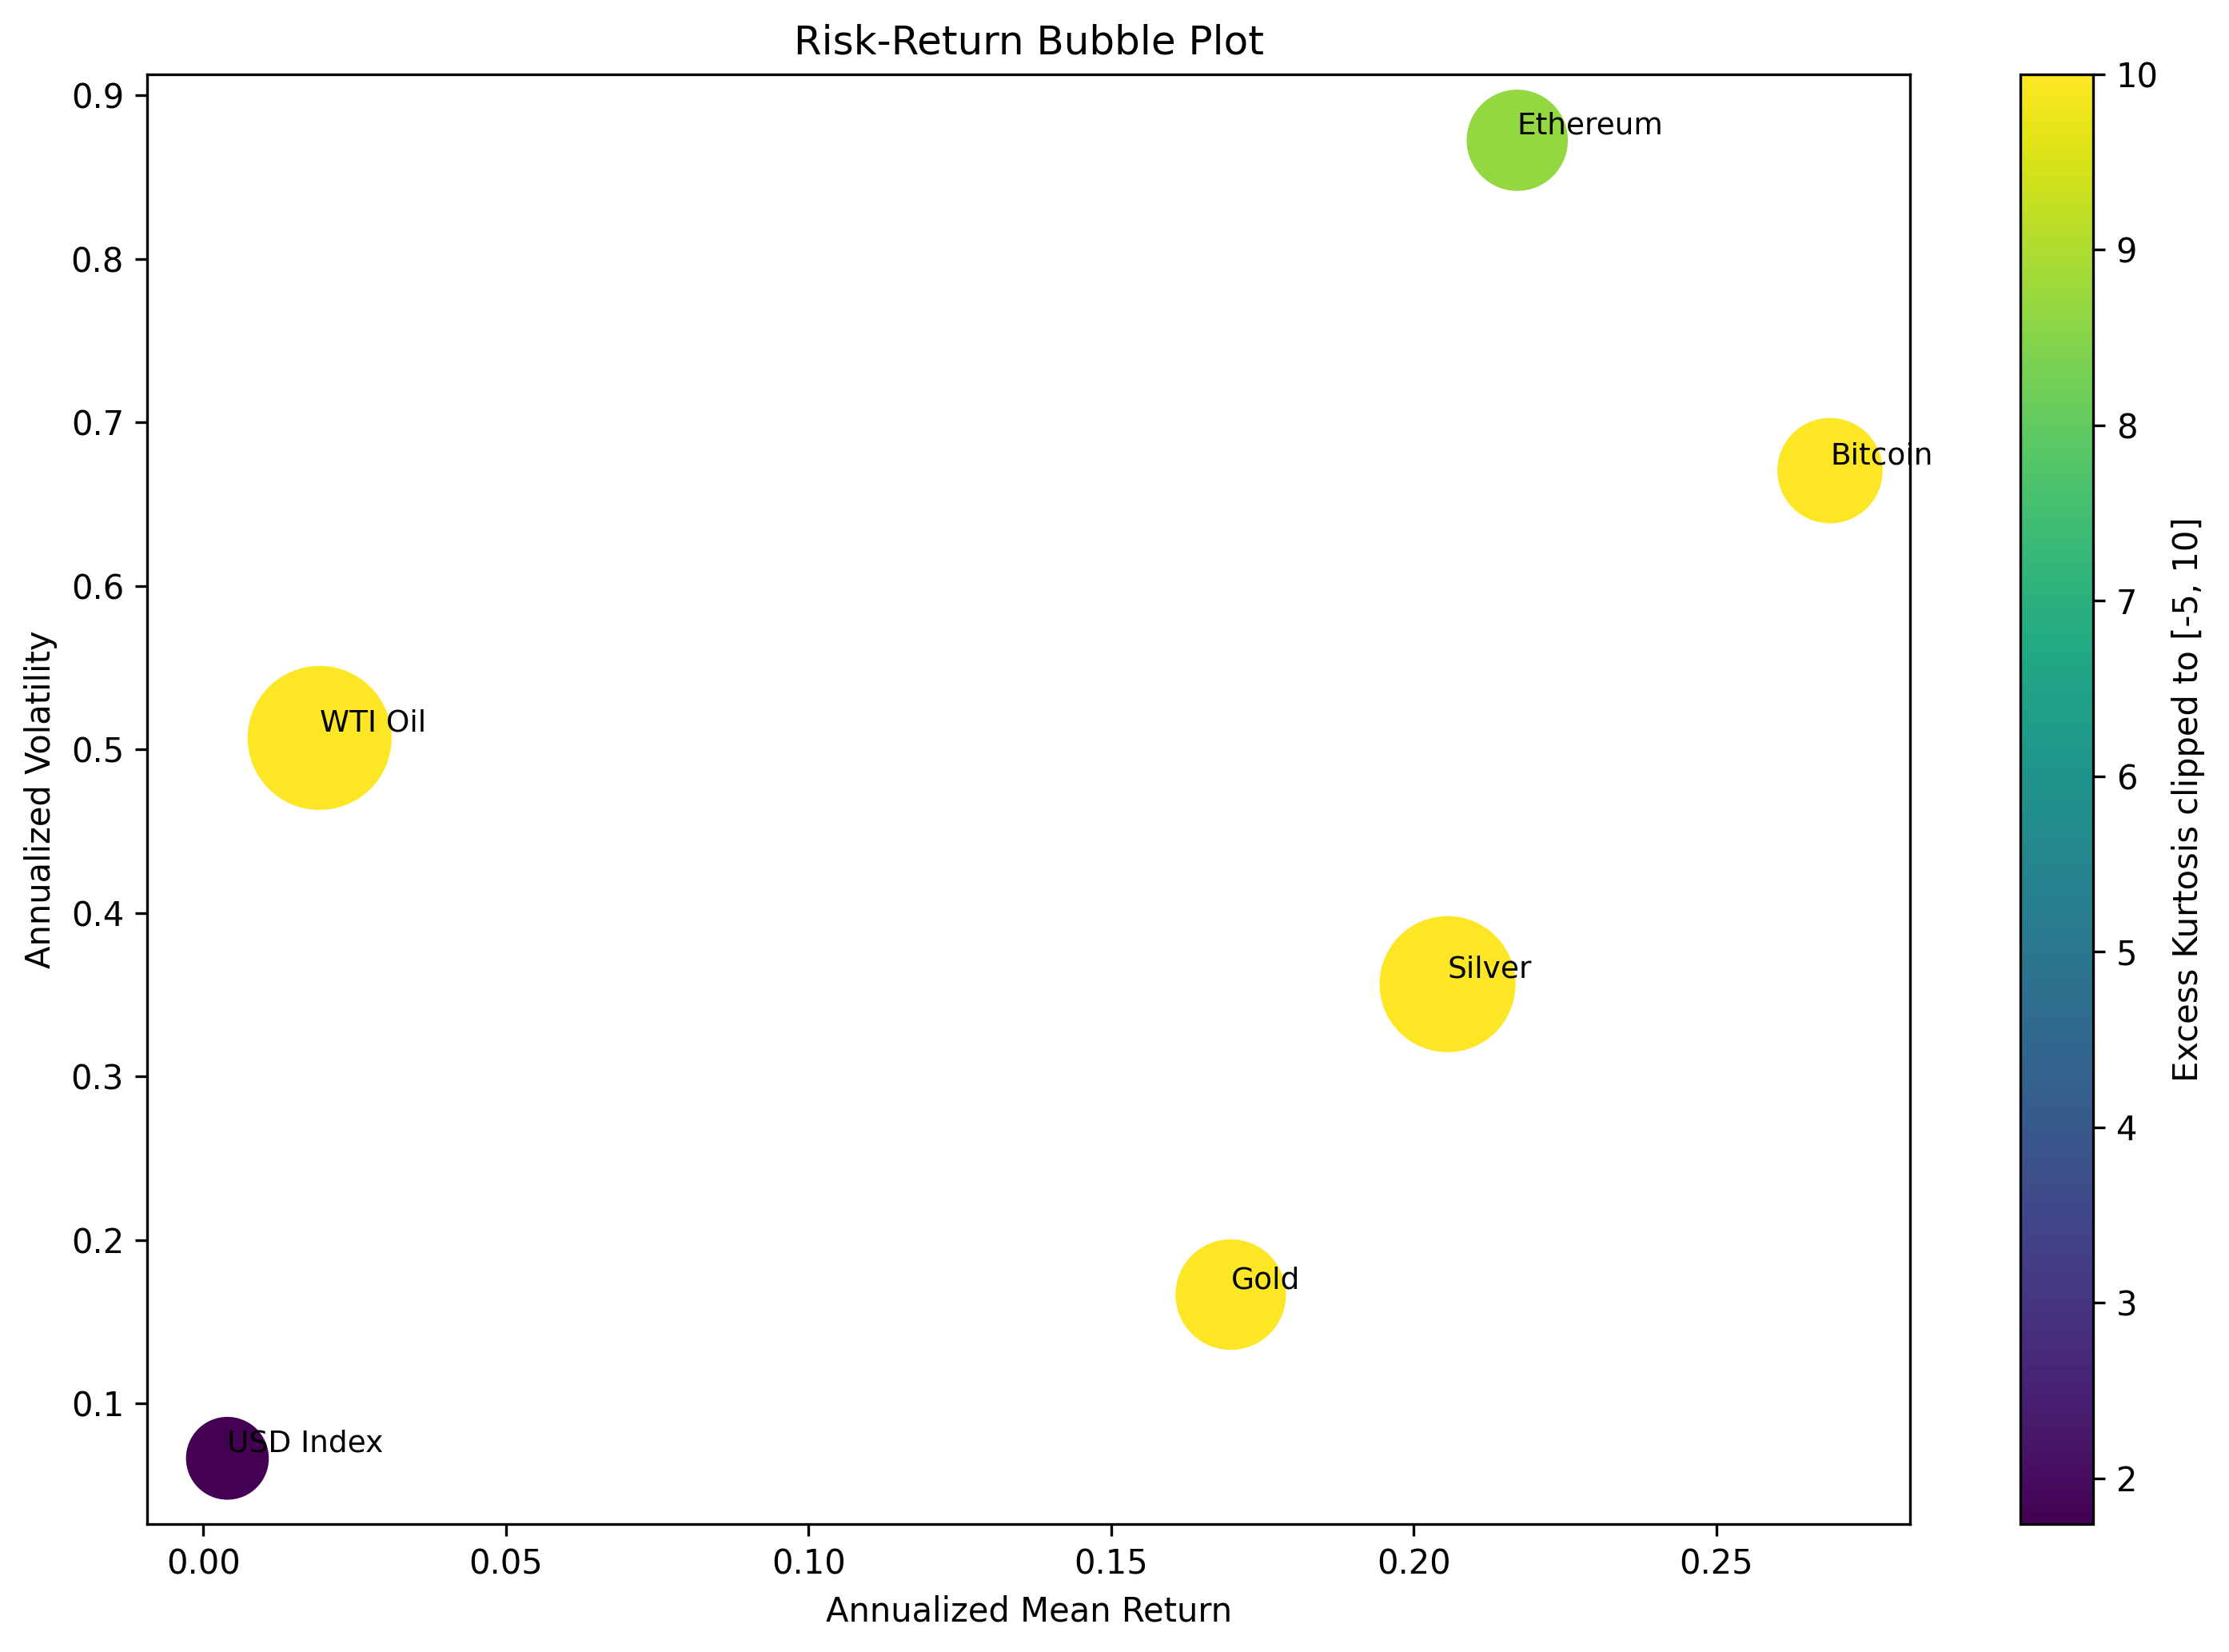
\includegraphics[width=0.58\textwidth]{EDA_plot/risk_return_bubble_plot.png}
    \caption{Risk-Return Bubble Plot}
    \label{fig:risk_return_bubble}
\end{figure}

Overall, the EDA shows that the six assets differ significantly in trend, volatility, correlation, and tail risk. These findings justify the use of engineered features such as lagged returns, momentum, rolling volatility, volatility ratios, rolling correlations, drawdowns, and extreme-return indicators in the later modeling sections.

\FloatBarrier

% ============================================================
% 4. Feature Engineering
% ============================================================

\section{Feature Engineering}

After the initial data cleaning and preprocessing steps, we constructed an extended feature set to provide richer predictive information for the machine learning models. The basic machine learning dataset already included lagged returns, rolling mean returns, rolling volatility features, and the next-day Bitcoin return target. In this section, we further add financial features designed to capture momentum, volatility changes, cross-asset relationships, market regimes, downside risk, and extreme return behavior.

The purpose of this step is not to repeat the preprocessing workflow, but to expand the information contained in the predictor matrix. Since financial returns are noisy and usually have weak linear predictability, a broader set of engineered features may help later models capture nonlinear patterns and changing market conditions.

\subsection{Extended Feature Groups}

The extended feature set includes seven major groups of engineered variables. Momentum features measure cumulative past log returns over multiple horizons. Volatility ratio features compare short-term volatility with longer-term volatility. Cross-asset features describe relative movement across asset classes, such as crypto spreads, metal spreads, and return differences between Bitcoin and the U.S. Dollar Index. Rolling correlation features measure whether the relationship between Bitcoin and other assets changes over time. In addition, volatility regime indicators, drawdown features, and extreme return flags are included to capture market stress and unusual return behavior.

\begin{table}[H]
\centering
\caption{Extended Feature Groups}
\begin{tabular}{ll}
\toprule
\textbf{Feature Group} & \textbf{Description} \\
\midrule
Momentum features & Rolling cumulative returns over 5, 10, 20, and 60 days \\
Volatility ratios & Short-term volatility relative to longer-term volatility \\
Cross-asset features & Return spreads and average returns across asset groups \\
Rolling correlations & Rolling correlations between Bitcoin and other assets \\
Volatility regimes & Indicators for high-volatility market states \\
Drawdown features & Declines from recent rolling maximum prices \\
Extreme return flags & Indicators for unusually large absolute returns \\
\bottomrule
\end{tabular}
\end{table}

These feature groups were selected because they represent different aspects of market behavior. Momentum features summarize recent trend direction, volatility ratios and regime indicators describe changing risk conditions, rolling correlations capture time-varying cross-asset relationships, and drawdown or extreme-return features measure market stress.

\subsection{Examples of Engineered Features}

To illustrate the engineered variables, Bitcoin is used as the main example because the primary target variable is the next-day Bitcoin log return. The following figure shows Bitcoin momentum features over different rolling windows.

\begin{figure}[H]
    \centering
    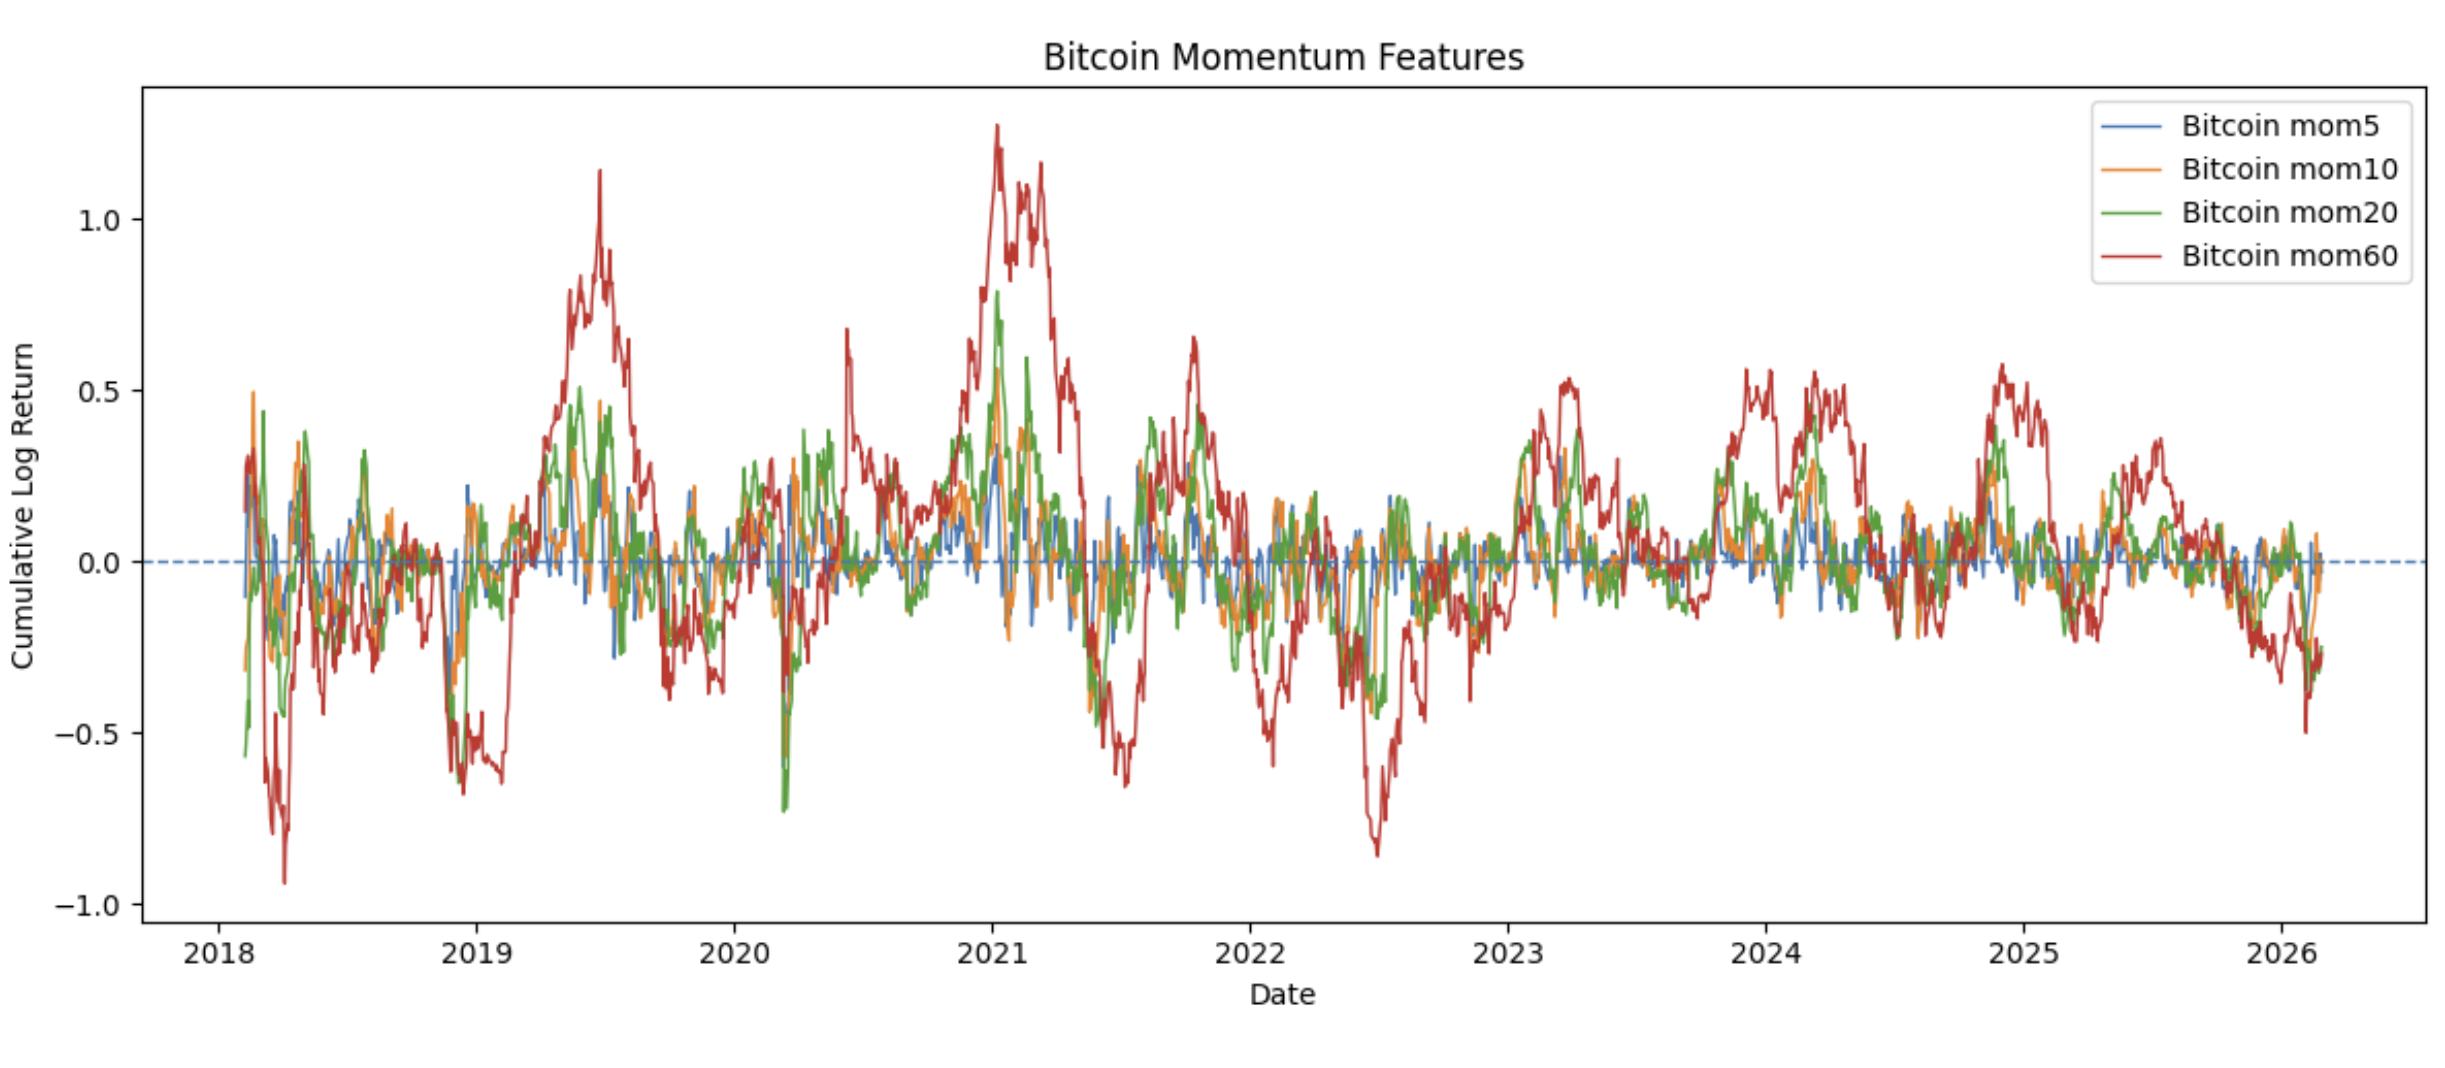
\includegraphics[width=0.82\textwidth]{feature_engineering_plot/Bitcoin Momentum Features.png}
    \caption{Bitcoin Momentum Features}
    \label{fig:bitcoin_momentum_features}
\end{figure}

The momentum features summarize cumulative past returns over short- and medium-term horizons. Positive values indicate recent upward price pressure, while negative values indicate recent downward pressure. These features help the models capture trend-following or reversal patterns in Bitcoin returns.

\begin{figure}[H]
    \centering
    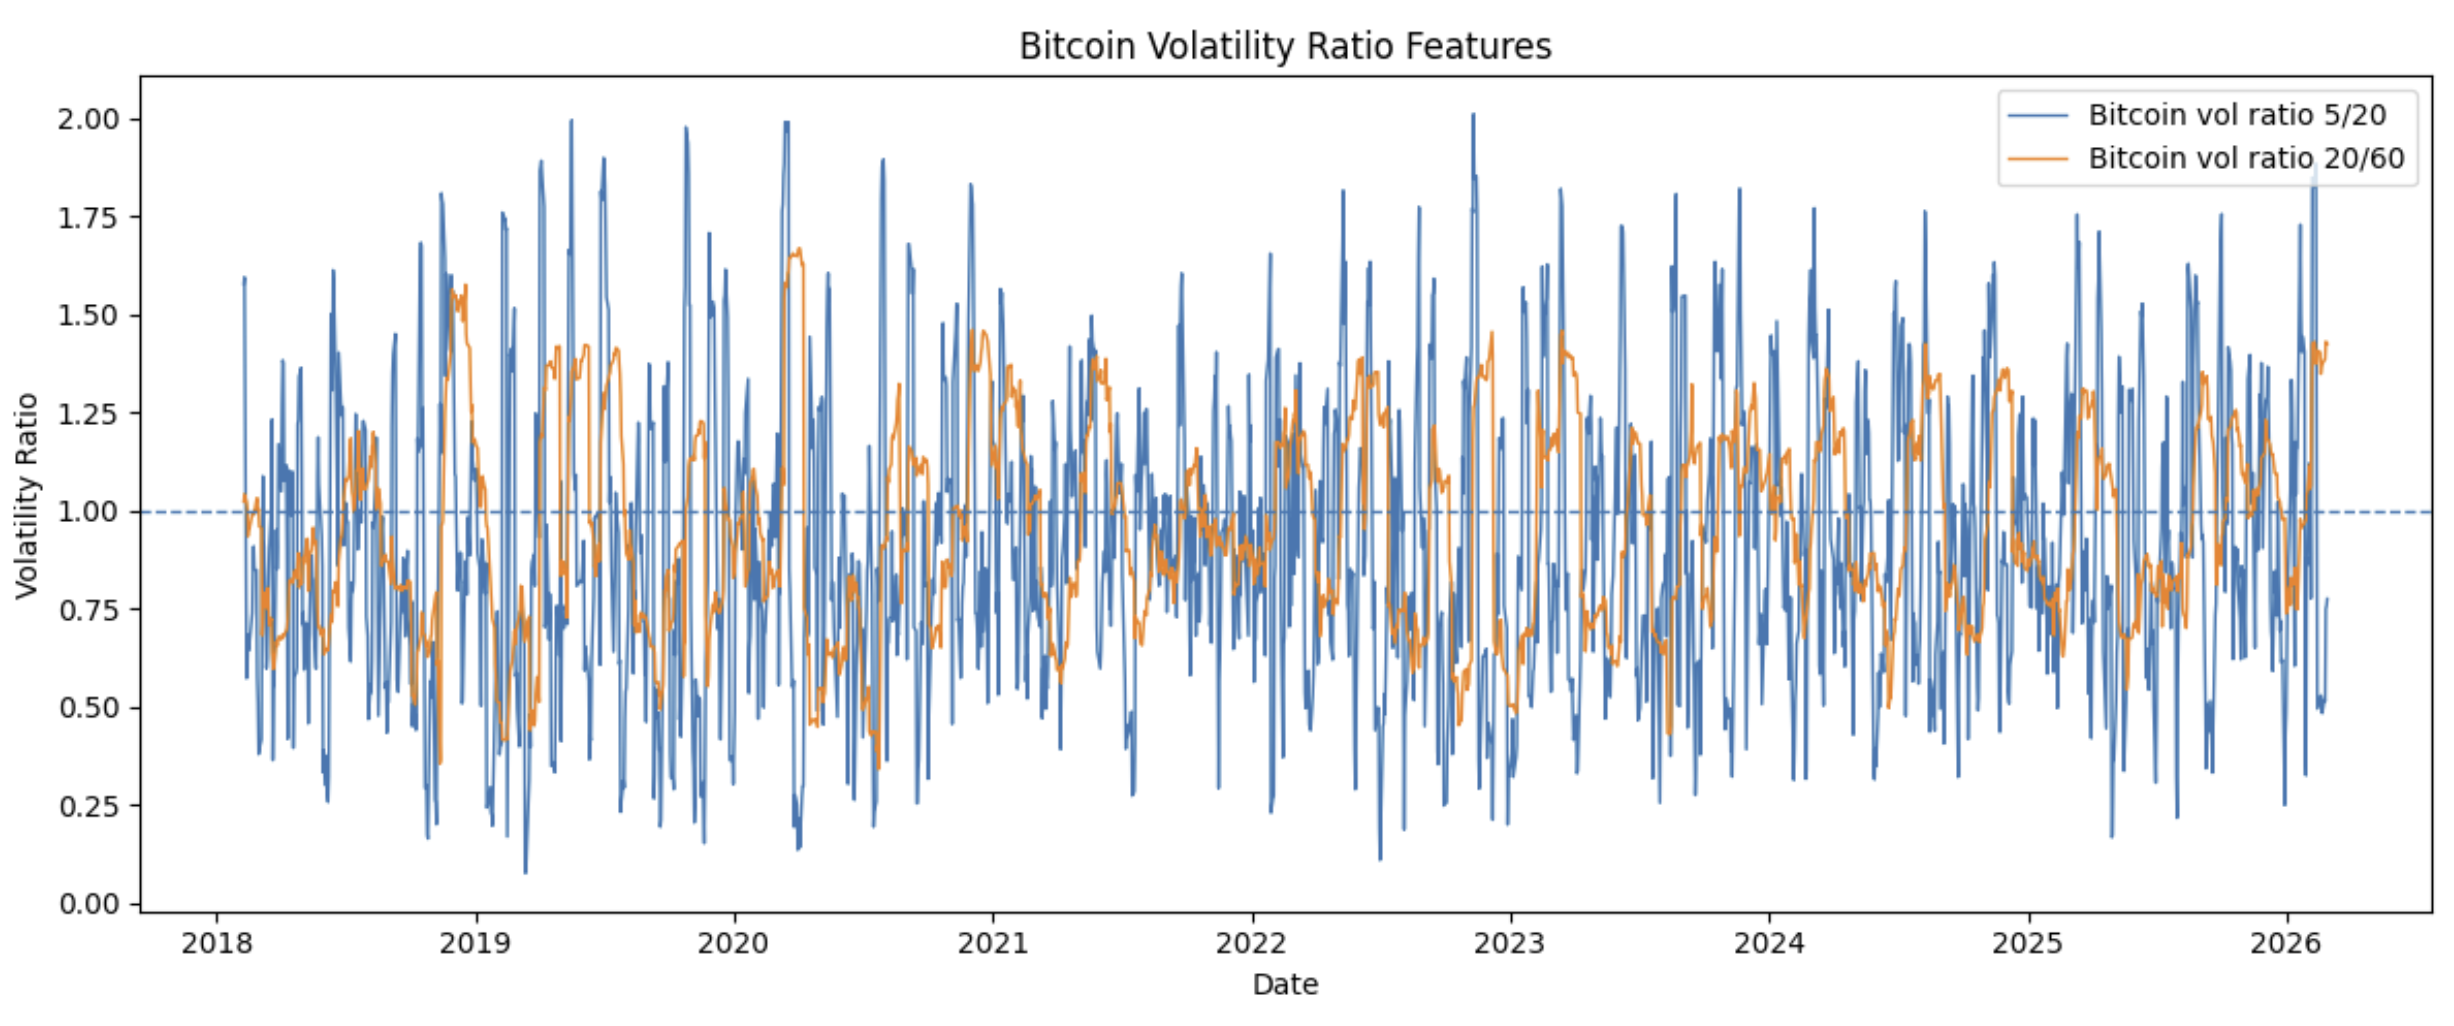
\includegraphics[width=0.82\textwidth]{feature_engineering_plot/Bitcoin Volatility Ratio Features.png}
    \caption{Bitcoin Volatility Ratio Features}
    \label{fig:bitcoin_volatility_ratio_features}
\end{figure}

The volatility ratio features compare recent volatility with longer-term volatility. Values above 1 indicate that short-term volatility is higher than the longer-term baseline, which may signal a transition into a more unstable market environment. These features are useful because financial assets often display volatility clustering.

\subsection{Final Extended Feature Set}

After constructing the extended features, they were combined with the original basic machine learning feature table. Rows with missing values caused by rolling-window calculations were removed. This reduction in sample size is expected because some variables require long historical windows, such as 60-day momentum, 252-day drawdown, and historical extreme return indicators.

\begin{table}[H]
\centering
\caption{Final Extended Feature Dataset Summary}
\begin{tabular}{ll}
\toprule
\textbf{Item} & \textbf{Result} \\
\midrule
Basic ML dataset shape & 2,063 rows $\times$ 61 columns \\
Extended features only & 2,084 rows $\times$ 75 columns \\
Final extended ML dataset & 1,832 rows $\times$ 136 columns \\
Extended predictor matrix & 1,832 rows $\times$ 135 features \\
Target variable & Bitcoin next-day log return \\
Training set & 1,282 rows $\times$ 135 features \\
Testing set & 550 rows $\times$ 135 features \\
\bottomrule
\end{tabular}
\end{table}

The final extended dataset contains 135 predictor variables and one target variable. The same chronological 70/30 train-test split and training-only \texttt{StandardScaler} procedure from the preprocessing section were applied to the extended feature matrix before unsupervised and supervised modeling. This avoids data leakage while keeping the modeling workflow consistent.

\subsection{Feature-Target Correlation}

We also examined the correlation between each engineered feature and the next-day Bitcoin return using only the training set. The results show that no single feature has a strong linear relationship with the target. This is expected in financial return prediction because daily returns usually have a low signal-to-noise ratio.

Therefore, the later supervised learning models are designed to combine many weak predictors rather than relying on one dominant feature. Linear models such as Ridge Regression provide a regularized benchmark, while tree-based models such as Random Forest and Hist Gradient Boosting can capture nonlinear interactions among the engineered features.

Overall, the extended feature engineering step provides a richer representation of market conditions. The final predictor matrix includes information about historical returns, changing volatility, cross-asset relationships, market stress, downside risk, and extreme return events. This extended feature set is then used in the following unsupervised and supervised learning sections.

% ============================================================
% 5. Unsupervised Analysis
% ============================================================

\section{Unsupervised Analysis}

After constructing the extended feature matrix, we applied unsupervised learning methods to identify hidden market structures. To avoid data leakage, the analysis was performed only on the scaled training feature matrix, which contained 1,282 observations and 135 engineered features.

\subsection{Principal Component Analysis}

Principal Component Analysis (PCA) was first used to reduce the high-dimensional feature space. The first two principal components explain 22.42\% of the total variance and are mainly used for visualization. Since the first ten principal components explain 53.60\% of the variance, we used the first ten PCs for K-Means clustering to preserve more information.

\begin{table}[H]
\centering
\caption{PCA Variance Summary}
\begin{tabular}{ll}
\toprule
\textbf{Principal Components} & \textbf{Explained Variance} \\
\midrule
PC1 & 13.61\% \\
PC2 & 8.81\% \\
PC1 + PC2 & 22.42\% \\
First 5 PCs & 38.95\% \\
First 10 PCs & 53.60\% \\
\bottomrule
\end{tabular}
\end{table}

\begin{figure}[!htbp]
    \centering
    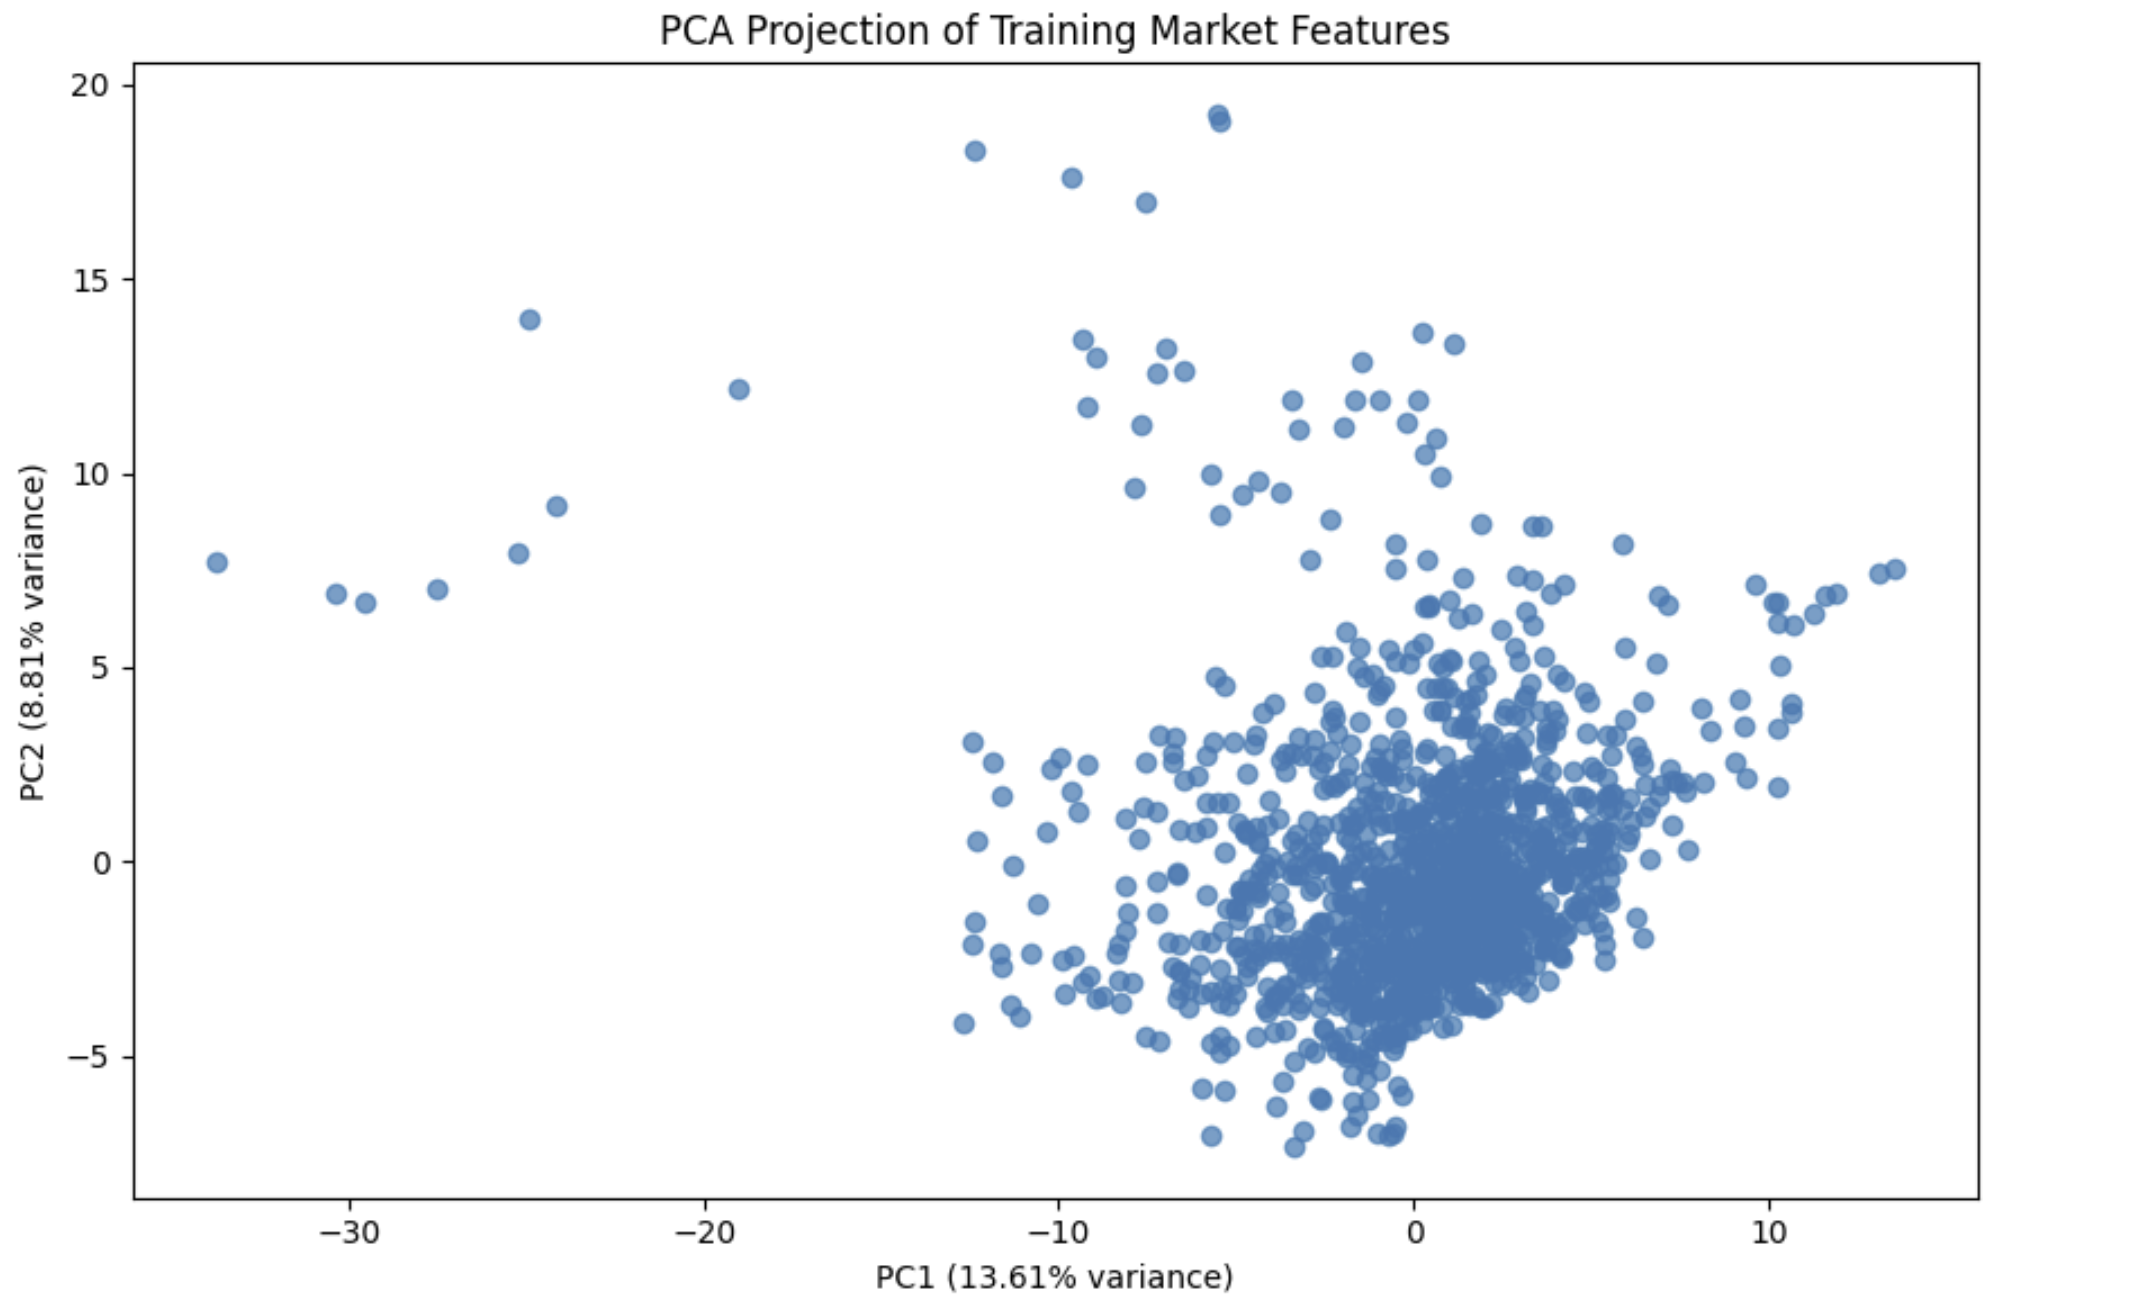
\includegraphics[width=0.66\textwidth]{unsupervised_analysis_plot/PCA Projection of Extended Financial Features.png}
    \caption{PCA Projection of Training Market Features}
    \label{fig:pca_projection}
\end{figure}

Figure~\ref{fig:pca_projection} shows the PCA projection of the training feature matrix. Most observations are concentrated near the center, while some points are farther away, suggesting the presence of unusual market conditions.

\FloatBarrier


\subsection{K-Means Clustering}

K-Means clustering was applied to the first ten principal components. Based on the elbow method and silhouette score, we selected two clusters as the final clustering structure.

\begin{table}[H]
\centering
\caption{Final K-Means Cluster Counts}
\begin{tabular}{lr}
\toprule
\textbf{Cluster} & \textbf{Number of Observations} \\
\midrule
Cluster 0 & 307 \\
Cluster 1 & 975 \\
\bottomrule
\end{tabular}
\end{table}

\begin{figure}[!htbp]
    \centering
    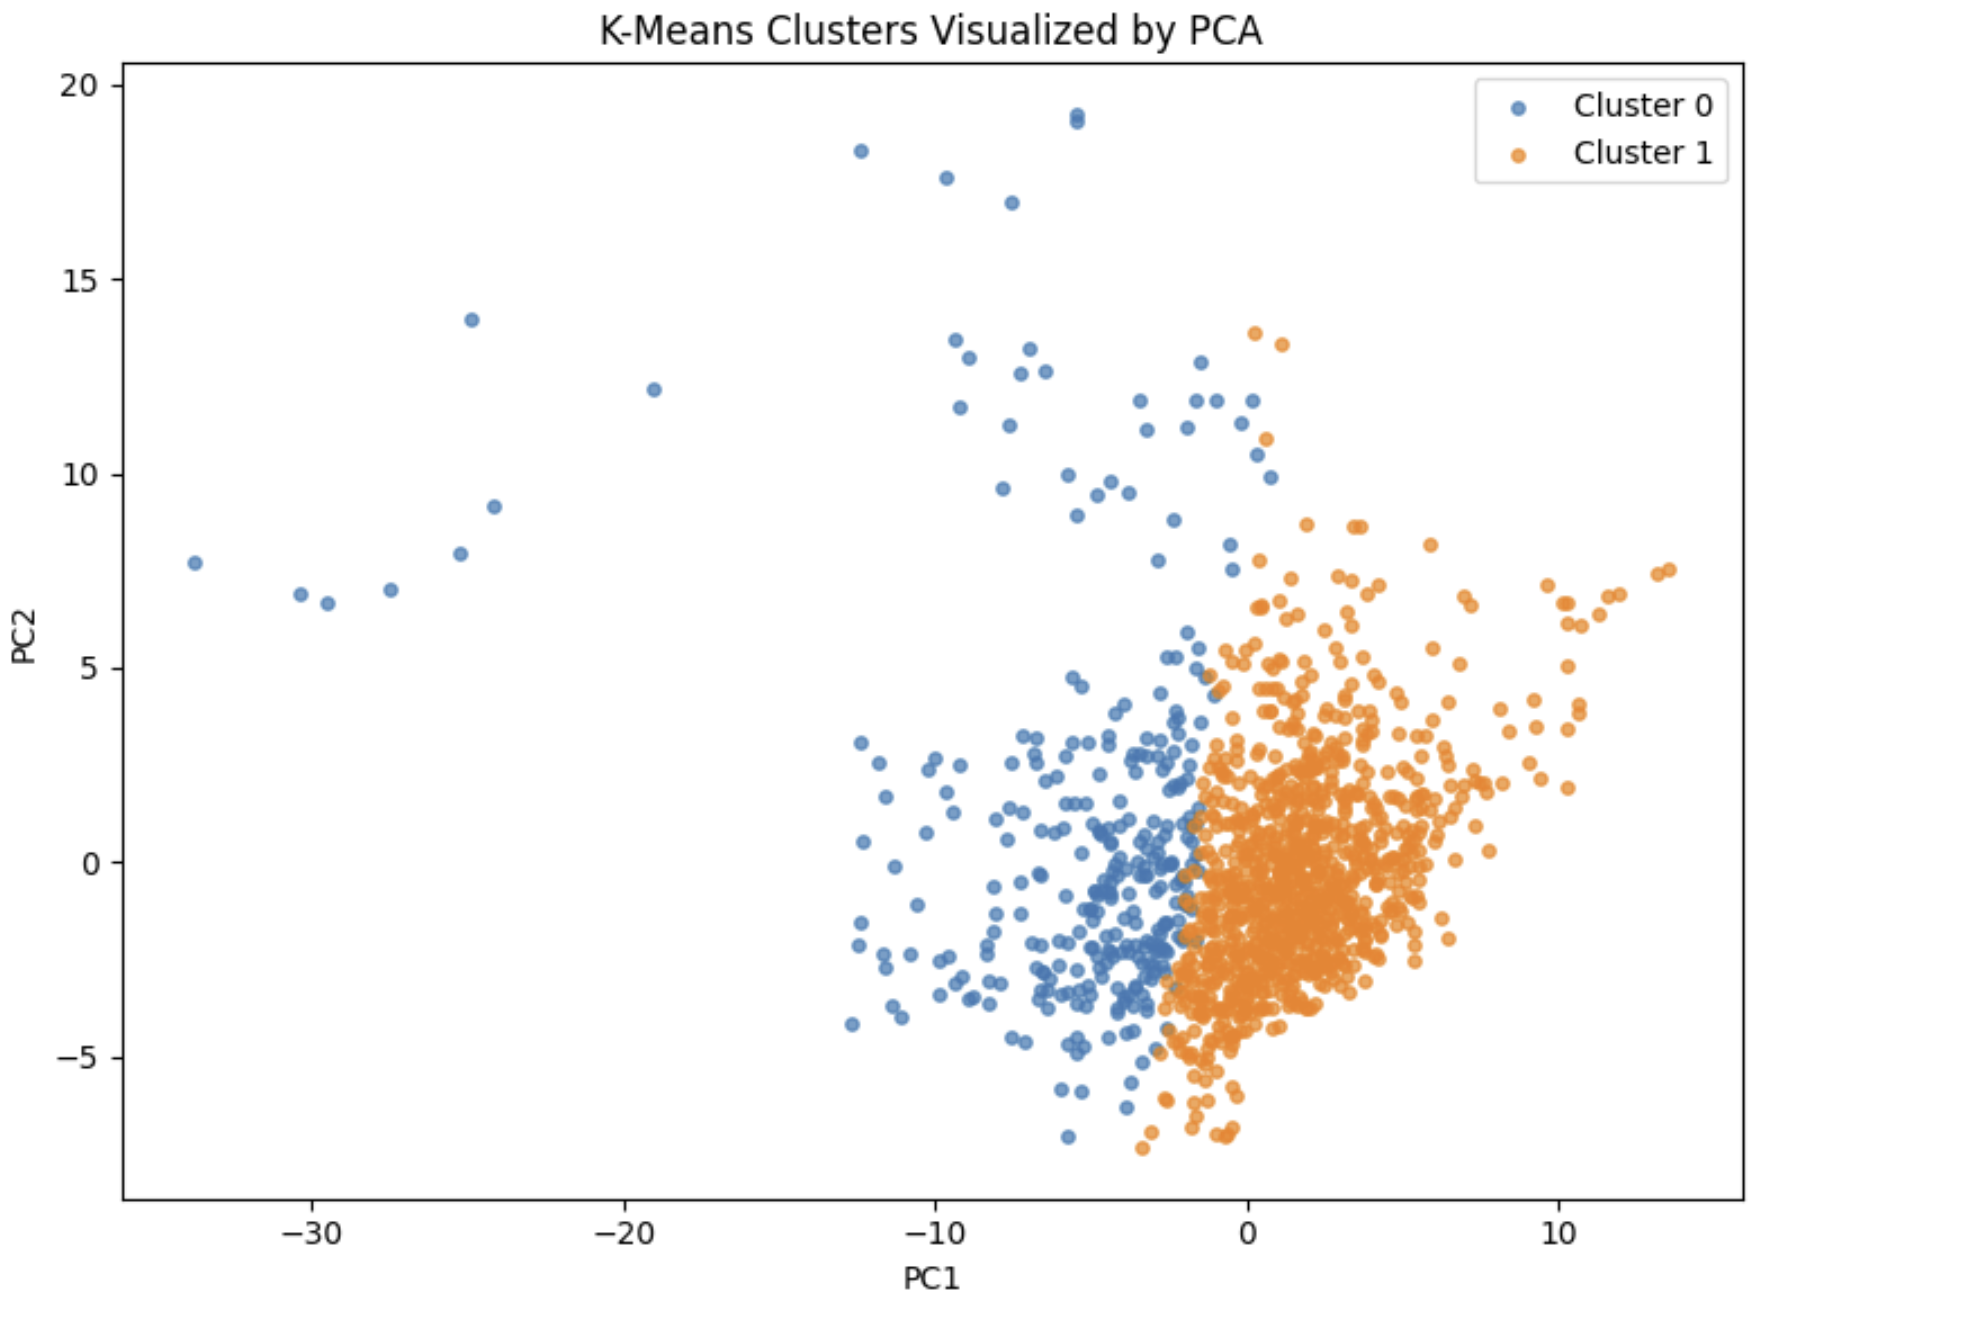
\includegraphics[width=0.66\textwidth]{unsupervised_analysis_plot/K-Means Clusters Visualized by PCA.png}
    \caption{K-Means Clusters Visualized by PCA}
    \label{fig:kmeans_clusters_pca}
\end{figure}

Figure~\ref{fig:kmeans_clusters_pca} shows that the two clusters are mainly separated along PC1. Cluster 0 contains fewer observations and is interpreted as a stress or high-volatility regime. Cluster 1 contains most observations and is interpreted as a normal or positive-momentum regime.

\FloatBarrier


\subsection{Cluster Interpretation}

To interpret the clusters, we compared selected feature averages across the two groups. Cluster 0 has more negative Bitcoin momentum, larger Bitcoin drawdowns, and higher volatility. In contrast, Cluster 1 has positive Bitcoin momentum, smaller drawdowns, and a higher average next-day Bitcoin return.

\begin{table}[H]
\centering
\caption{Selected Cluster Interpretation Results}
\begin{tabular}{lrr}
\toprule
\textbf{Feature} & \textbf{Cluster 0} & \textbf{Cluster 1} \\
\midrule
Bitcoin 20-day momentum & -0.1805 & 0.0943 \\
Bitcoin 60-day momentum & -0.2314 & 0.1737 \\
Bitcoin 60-day drawdown & -0.3224 & -0.1195 \\
Bitcoin 252-day drawdown & -0.5183 & -0.2690 \\
Bitcoin 20-day volatility & 0.0497 & 0.0364 \\
Ethereum 20-day volatility & 0.0674 & 0.0459 \\
Bitcoin next-day return & -0.0003 & 0.0020 \\
\bottomrule
\end{tabular}
\end{table}

Overall, the cluster interpretation suggests that Cluster 0 represents a \textbf{stress / high-volatility regime}, while Cluster 1 represents a \textbf{normal / positive-momentum regime}. Although the target variable was not used in clustering, the two regimes show different average future Bitcoin returns.

\FloatBarrier


\subsection{Isolation Forest Outlier Detection}

We also applied Isolation Forest to detect unusual market observations. The contamination level was set to 0.05, so approximately 5\% of the training observations were expected to be identified as outliers.

\begin{table}[H]
\centering
\caption{Isolation Forest Outlier Results}
\begin{tabular}{lr}
\toprule
\textbf{Observation Type} & \textbf{Count} \\
\midrule
Normal observations & 1217 \\
Outliers & 65 \\
\bottomrule
\end{tabular}
\end{table}

Most outliers are located in Cluster 0, which supports the interpretation of Cluster 0 as a market stress regime.

\begin{table}[H]
\centering
\caption{Outlier Distribution by Cluster}
\begin{tabular}{lrr}
\toprule
\textbf{Cluster} & \textbf{Normal Observations} & \textbf{Outliers} \\
\midrule
Cluster 0 & 256 & 51 \\
Cluster 1 & 961 & 14 \\
\bottomrule
\end{tabular}
\end{table}

\begin{figure}[!htbp]
    \centering
    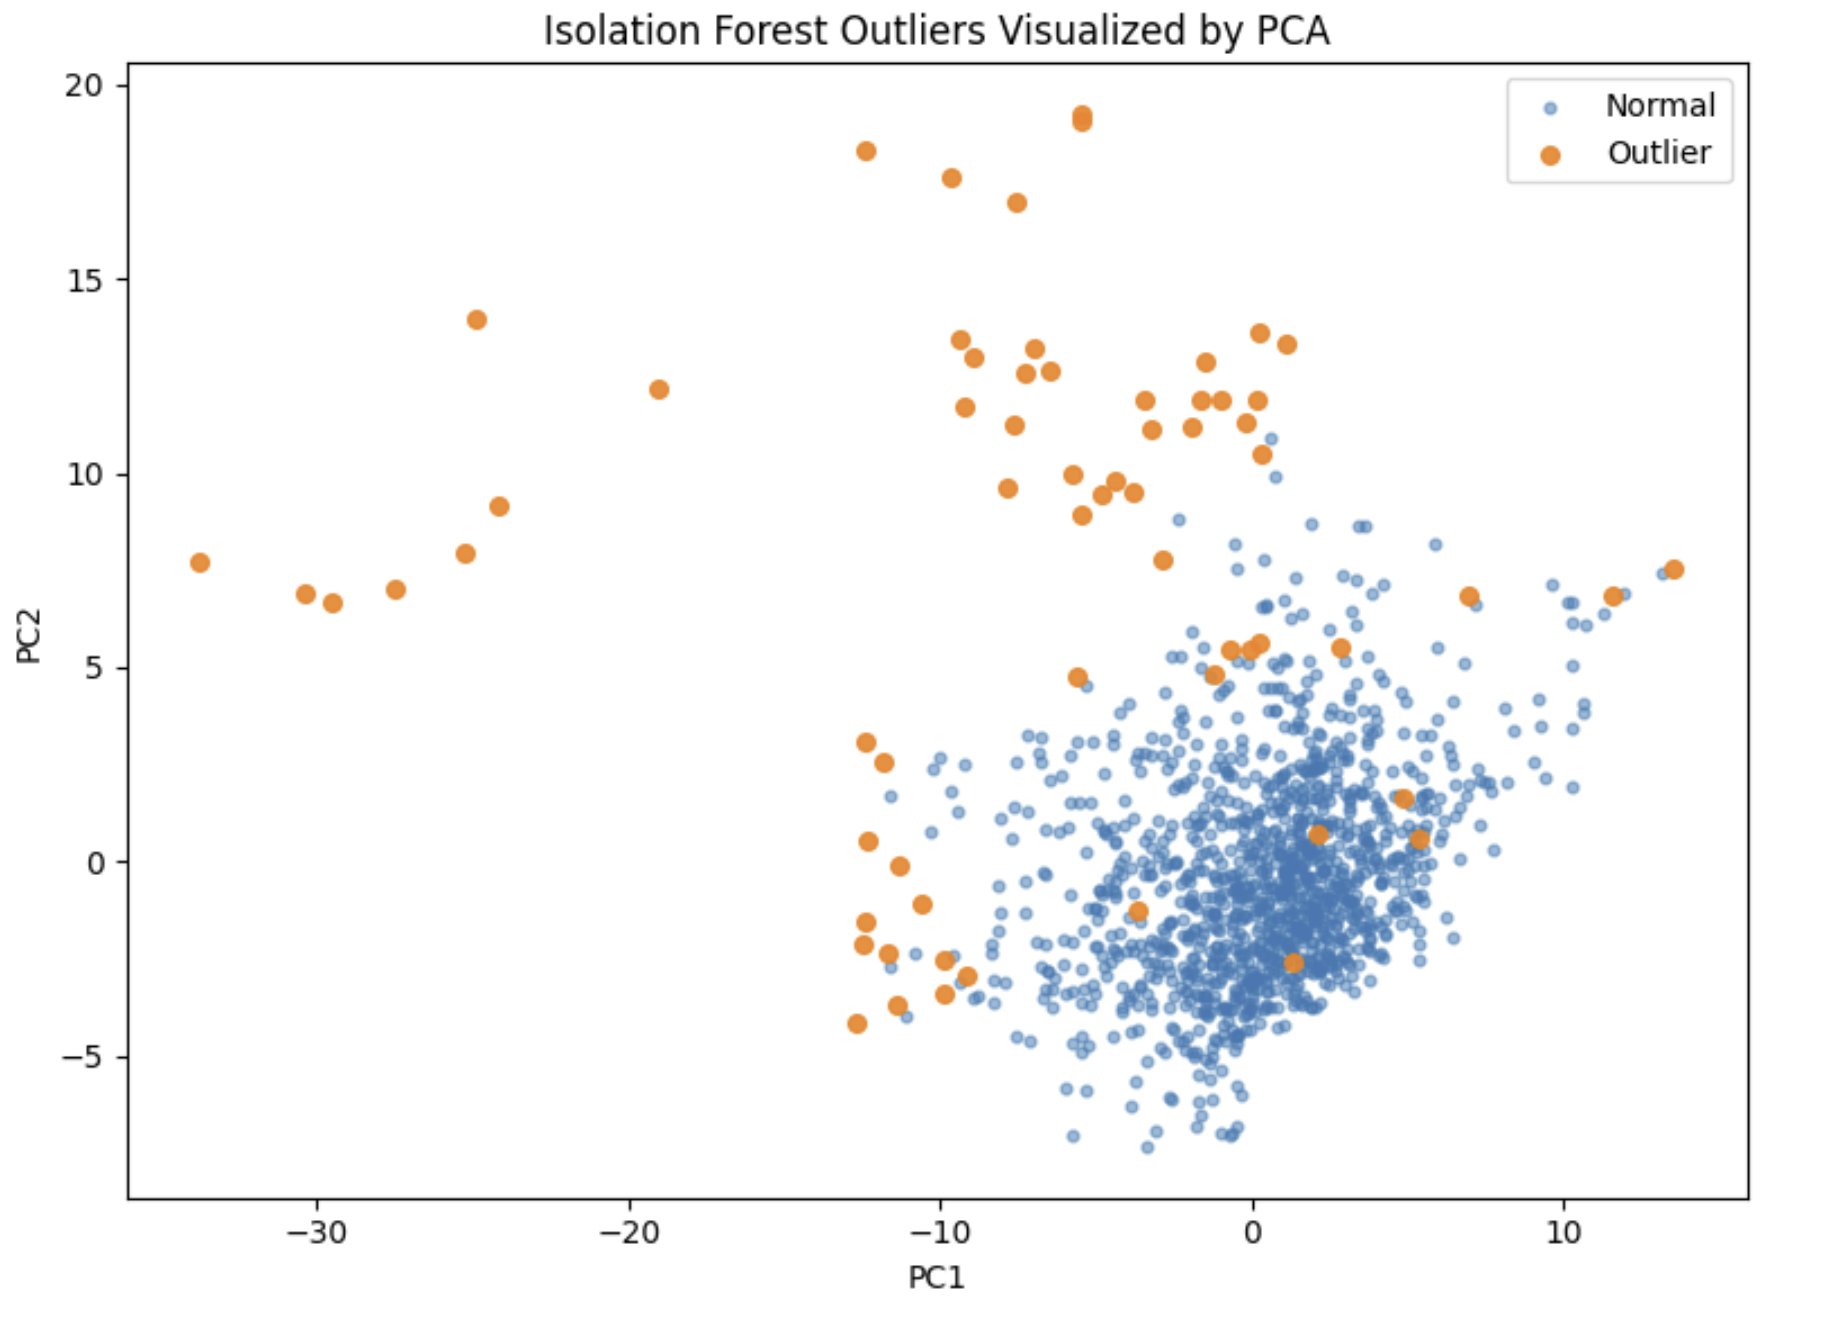
\includegraphics[width=0.66\textwidth]{unsupervised_analysis_plot/Isolation Forest Outliers Visualized by PCA.png}
    \caption{Isolation Forest Outliers Visualized by PCA}
    \label{fig:isolation_forest_outliers}
\end{figure}

Figure~\ref{fig:isolation_forest_outliers} shows that the detected outliers are mostly away from the dense central region. Many of the most unusual observations occur around March 2020, which is consistent with the COVID-19 market crash period.

Overall, the unsupervised analysis shows that the engineered features capture meaningful market structure. PCA summarizes the feature space, K-Means identifies two interpretable market regimes, and Isolation Forest highlights unusual stress periods.

\FloatBarrier

% ============================================================
% 6. Supervised Machine Learning Models
% ============================================================

\section{Supervised Machine Learning Models}

This section applies supervised machine learning models to predict the next-day log return of each asset. Based on the extended feature engineering dataset, three different models were trained and compared: Ridge Regression, Random Forest, and Hist Gradient Boosting. These models were applied separately to the six assets: Gold, Silver, WTI Oil, USD Index, Bitcoin, and Ethereum. The purpose of this section is to compare the predictive performance of linear and nonlinear models and identify the most suitable model for each asset.

\subsection{Model Setup}

Let $P_t^{(a)}$ denote the price of asset $a$ at time $t$. The prediction target is the next-day log return, defined as

\begin{equation}
y_{t+1}^{(a)} = r_{t+1}^{(a)}
=
\log\left(\frac{P_{t+1}^{(a)}}{P_t^{(a)}}\right).
\end{equation}

For each asset, the explanatory variables are the engineered market features at time $t$, including lagged returns, rolling mean and volatility features, momentum variables, cross-asset features, rolling correlations, drawdown indicators, and extreme-return indicators. The supervised learning task can therefore be written as

\begin{equation}
\hat{y}_{t+1}^{(a)} = f(X_t),
\end{equation}

where $X_t$ is the feature vector at time $t$ and $f(\cdot)$ denotes the machine learning model.

Because this is a time series forecasting problem, the dataset was split chronologically rather than randomly. The first 70\% of observations were used as the training set, and the remaining 30\% were used as the testing set. Hyperparameter tuning was conducted using \texttt{TimeSeriesSplit} with 5 folds in order to preserve the time ordering of the observations and reduce the risk of data leakage.

\subsection{Ridge Regression}

Ridge Regression was used as the baseline linear model. It extends ordinary least squares by adding an $L_2$ penalty on the coefficient vector, which helps reduce overfitting and improve model stability when the feature set is large and potentially correlated.

The Ridge Regression estimator solves the following optimization problem:

\begin{equation}
\hat{\beta}
=
\arg\min_{\beta}
\left[
\sum_{i=1}^{n}
(y_i - \beta_0 - X_i^\top \beta)^2
+
\lambda \sum_{j=1}^{p} \beta_j^2
\right],
\end{equation}

where $\lambda \ge 0$ is the regularization parameter. A larger $\lambda$ produces stronger shrinkage of the regression coefficients. In this project, Ridge Regression was implemented inside a pipeline with \texttt{StandardScaler}, so the features were standardized before model fitting. The regularization parameter $\lambda$, implemented as \texttt{alpha}, was selected using grid search over the following candidate values:

\[
\{0.1,\ 1,\ 10,\ 50,\ 100,\ 500,\ 1000\}.
\]

Ridge Regression is useful because it provides an interpretable linear benchmark. If Ridge performs poorly compared with tree-based models, this suggests that the prediction problem may involve nonlinear relationships or feature interactions.

\subsection{Random Forest}

Random Forest is an ensemble tree-based model that combines many decision trees to improve predictive accuracy and robustness. Each tree is trained on a bootstrap sample of the training data, and at each split only a random subset of features is considered. The final prediction is obtained by averaging the predictions from all trees:

\begin{equation}
\hat{y}(X)
=
\frac{1}{B}
\sum_{b=1}^{B}
T_b(X),
\end{equation}

where $T_b(\cdot)$ denotes the $b$-th regression tree and $B$ is the number of trees.

Random Forest can capture nonlinear relationships and feature interactions without requiring a strict parametric functional form. This is especially useful for financial data, where the relationship between engineered predictors and future returns may be complex, unstable, and nonlinear.

In this project, the following Random Forest hyperparameters were tuned using randomized search:

\begin{itemize}
    \item number of trees: \texttt{n\_estimators} $\in \{300, 500\}$,
    \item maximum tree depth: \texttt{max\_depth} $\in \{3, 5, 8, \texttt{None}\}$,
    \item minimum samples per leaf: \texttt{min\_samples\_leaf} $\in \{5, 10, 20\}$,
    \item number of features per split: \texttt{max\_features} $\in \{\texttt{sqrt}, 0.3, 0.5\}$.
\end{itemize}

Because of its flexibility, Random Forest is expected to perform well when the engineered features contain nonlinear predictive signals.

\subsection{Hist Gradient Boosting}

Hist Gradient Boosting is another tree-based ensemble model, but unlike Random Forest, it builds trees sequentially. Each new tree is trained to reduce the errors made by the previous ensemble. The general boosting structure can be written as

\begin{equation}
F_m(X) = F_{m-1}(X) + \nu h_m(X),
\end{equation}

where $F_m(\cdot)$ is the boosted model after $m$ iterations, $h_m(\cdot)$ is the newly fitted tree, and $\nu$ is the learning rate.

The histogram-based implementation makes this method computationally efficient for structured tabular datasets. Hist Gradient Boosting can capture nonlinear patterns and complex interactions, and it often performs strongly on engineered feature matrices.

In this project, the following hyperparameters were tuned using randomized search:

\begin{itemize}
    \item learning rate: \texttt{learning\_rate} $\in \{0.01, 0.03, 0.05, 0.1\}$,
    \item number of boosting iterations: \texttt{max\_iter} $\in \{100, 200, 300\}$,
    \item maximum number of leaf nodes: \texttt{max\_leaf\_nodes} $\in \{15, 31, 63\}$,
    \item minimum samples per leaf: \texttt{min\_samples\_leaf} $\in \{10, 20, 40\}$,
    \item regularization strength: \texttt{l2\_regularization} $\in \{0.0, 0.01, 0.1\}$.
\end{itemize}

This model was included to represent a more advanced nonlinear boosting approach and to compare its performance with both Ridge Regression and Random Forest.

\subsection{Evaluation Metrics}

For each asset, the three models were evaluated on the testing set. The prediction performance was measured using MSE, RMSE, MAE, $R^2$, and directional accuracy.

\paragraph{Mean Squared Error (MSE)}
\begin{equation}
\text{MSE}
=
\frac{1}{n}
\sum_{i=1}^{n}
(y_i - \hat{y}_i)^2.
\end{equation}

\paragraph{Root Mean Squared Error (RMSE)}
\begin{equation}
\text{RMSE}
=
\sqrt{
\frac{1}{n}
\sum_{i=1}^{n}
(y_i - \hat{y}_i)^2
}.
\end{equation}

\paragraph{Mean Absolute Error (MAE)}
\begin{equation}
\text{MAE}
=
\frac{1}{n}
\sum_{i=1}^{n}
|y_i - \hat{y}_i|.
\end{equation}

\paragraph{$R^2$ Score}
\begin{equation}
R^2
=
1
-
\frac{
\sum_{i=1}^{n}(y_i - \hat{y}_i)^2
}{
\sum_{i=1}^{n}(y_i - \bar{y})^2
}.
\end{equation}

\paragraph{Directional Accuracy}
\begin{equation}
\text{Directional Accuracy}
=
\frac{1}{n}
\sum_{i=1}^{n}
\mathbf{1}
\left(
\operatorname{sign}(y_i)
=
\operatorname{sign}(\hat{y}_i)
\right).
\end{equation}

MSE, RMSE, and MAE measure the magnitude of prediction errors. The $R^2$ score measures the relative goodness of fit compared with a mean prediction baseline. Directional accuracy evaluates whether the model correctly predicts the sign of the next-day return, which is especially relevant for financial forecasting.

% ============================================================
% 6.6 Return Prediction Plots for All Models
% ============================================================

\subsection{Return Prediction Plots for All Models}

The supervised learning models in this project were trained to predict next-day log returns. Therefore, before converting the predicted returns into price paths, we first examine the actual and predicted return series directly. These return prediction plots provide a more direct evaluation of the model output because the target variable used in training is return, not price level.

Compared with price prediction plots, return prediction plots usually look more noisy because daily returns fluctuate around zero and contain many short-term shocks. However, these plots are important because they show whether the models can capture the direction, volatility, and extreme movements of the return series. The price prediction plots in the next section are easier to interpret visually, but they are accumulated results transformed from predicted returns. Therefore, both return plots and price plots are useful: return plots evaluate the original machine learning target, while price plots show the practical financial implication of the forecasts.

% ------------------------------------------------------------
% Figure: Return Prediction Plots for Precious Metals
% ------------------------------------------------------------

\begin{figure}[H]
    \centering
    \captionsetup[subfigure]{skip=4pt}
    \setlength{\abovecaptionskip}{5pt}
    \setlength{\belowcaptionskip}{3pt}

    % ---------------- Gold ----------------
    \begin{subfigure}[t]{0.29\textwidth}
        \centering
        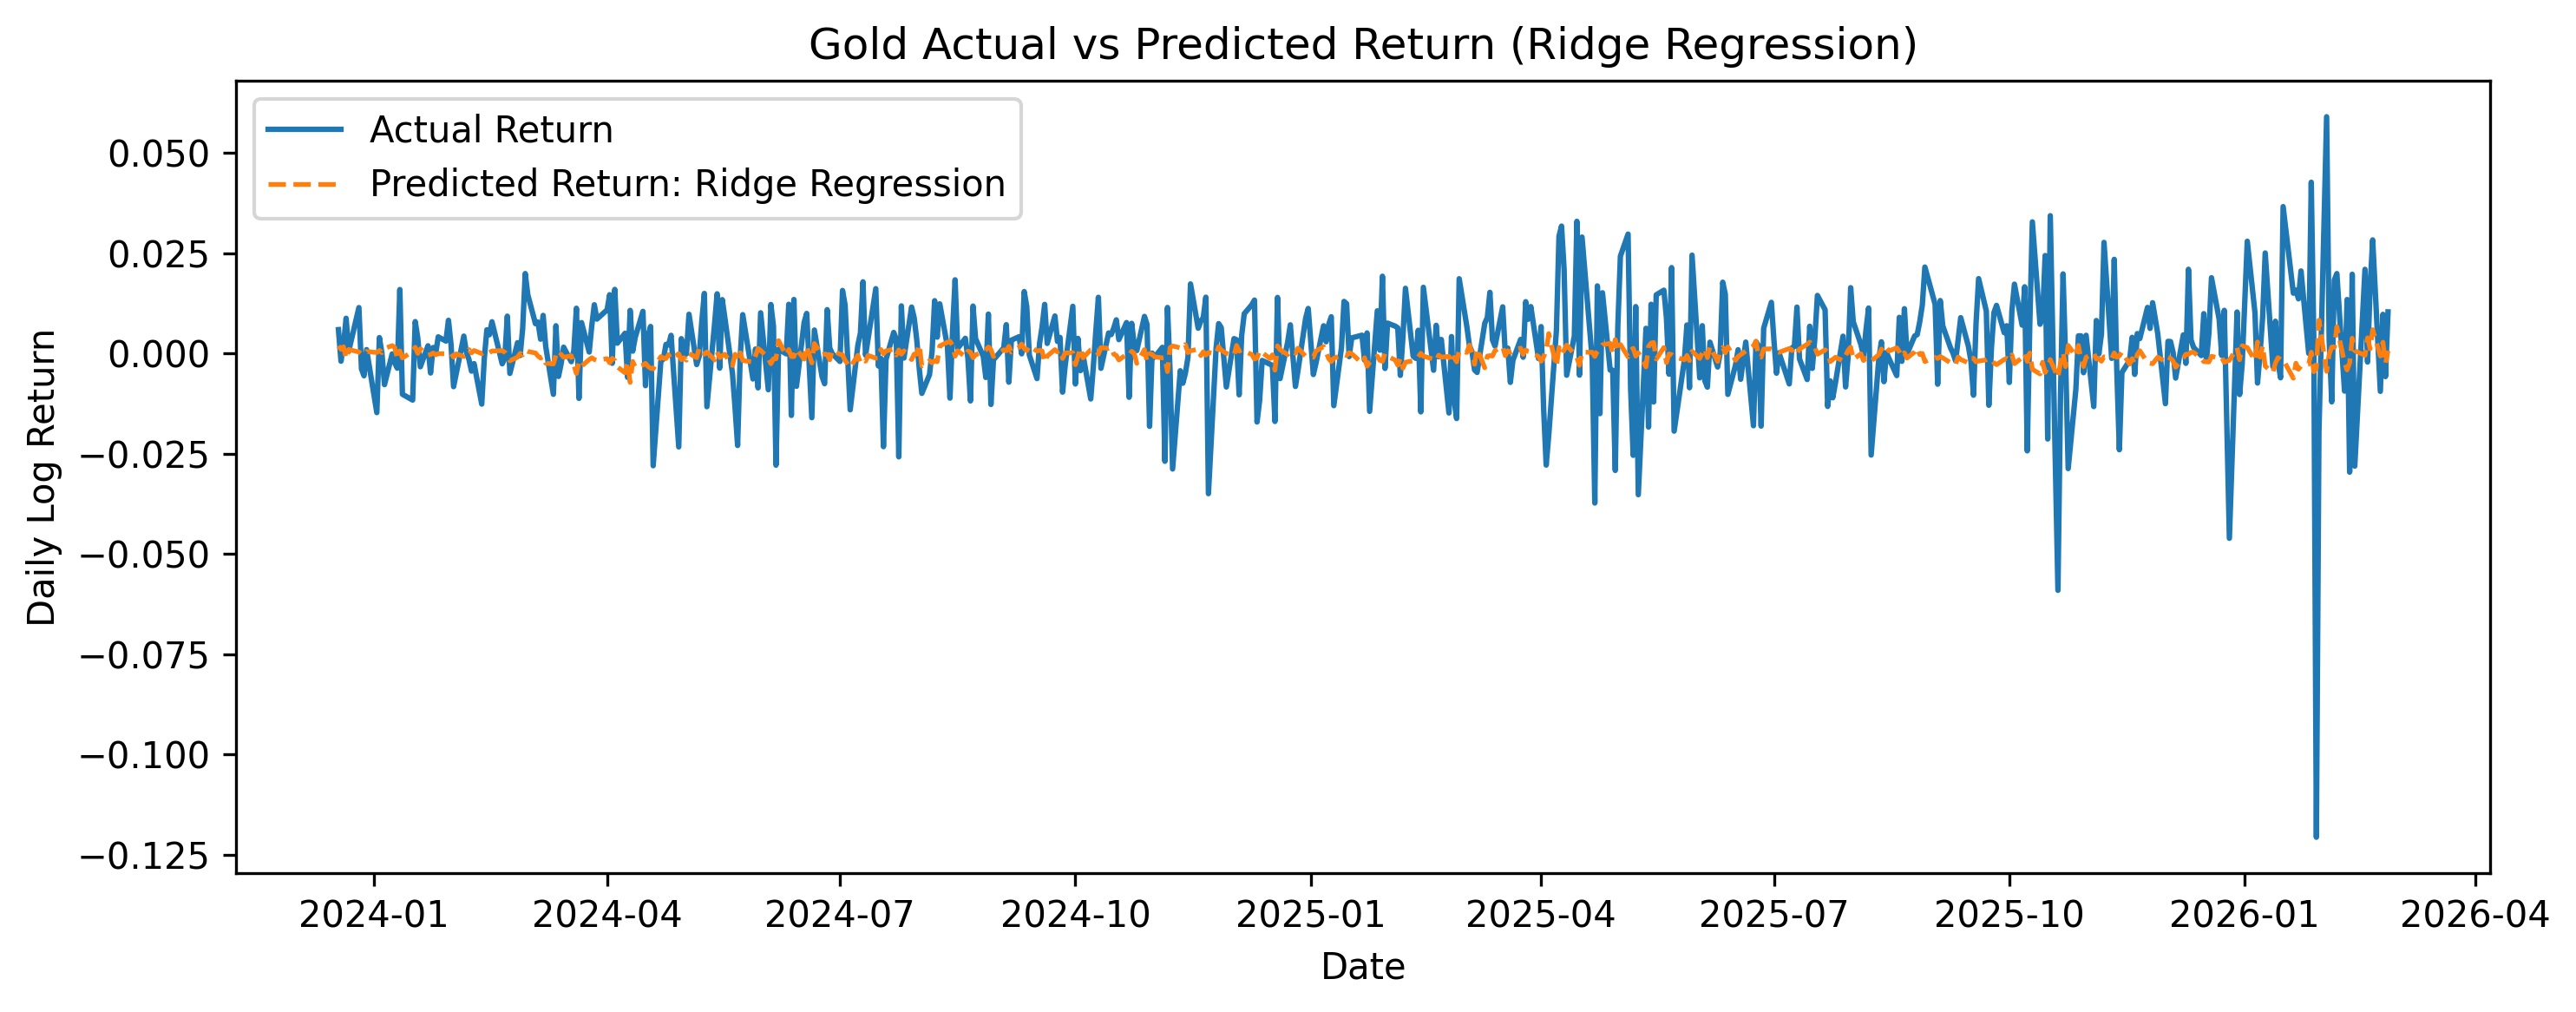
\includegraphics[width=\textwidth, trim=0 6 0 6, clip]{modeling_return_plot/Gold_Ridge_Regression_return_prediction.png}
        \caption{Gold -- Ridge}
    \end{subfigure}
    \hspace{0.025\textwidth}
    \begin{subfigure}[t]{0.29\textwidth}
        \centering
        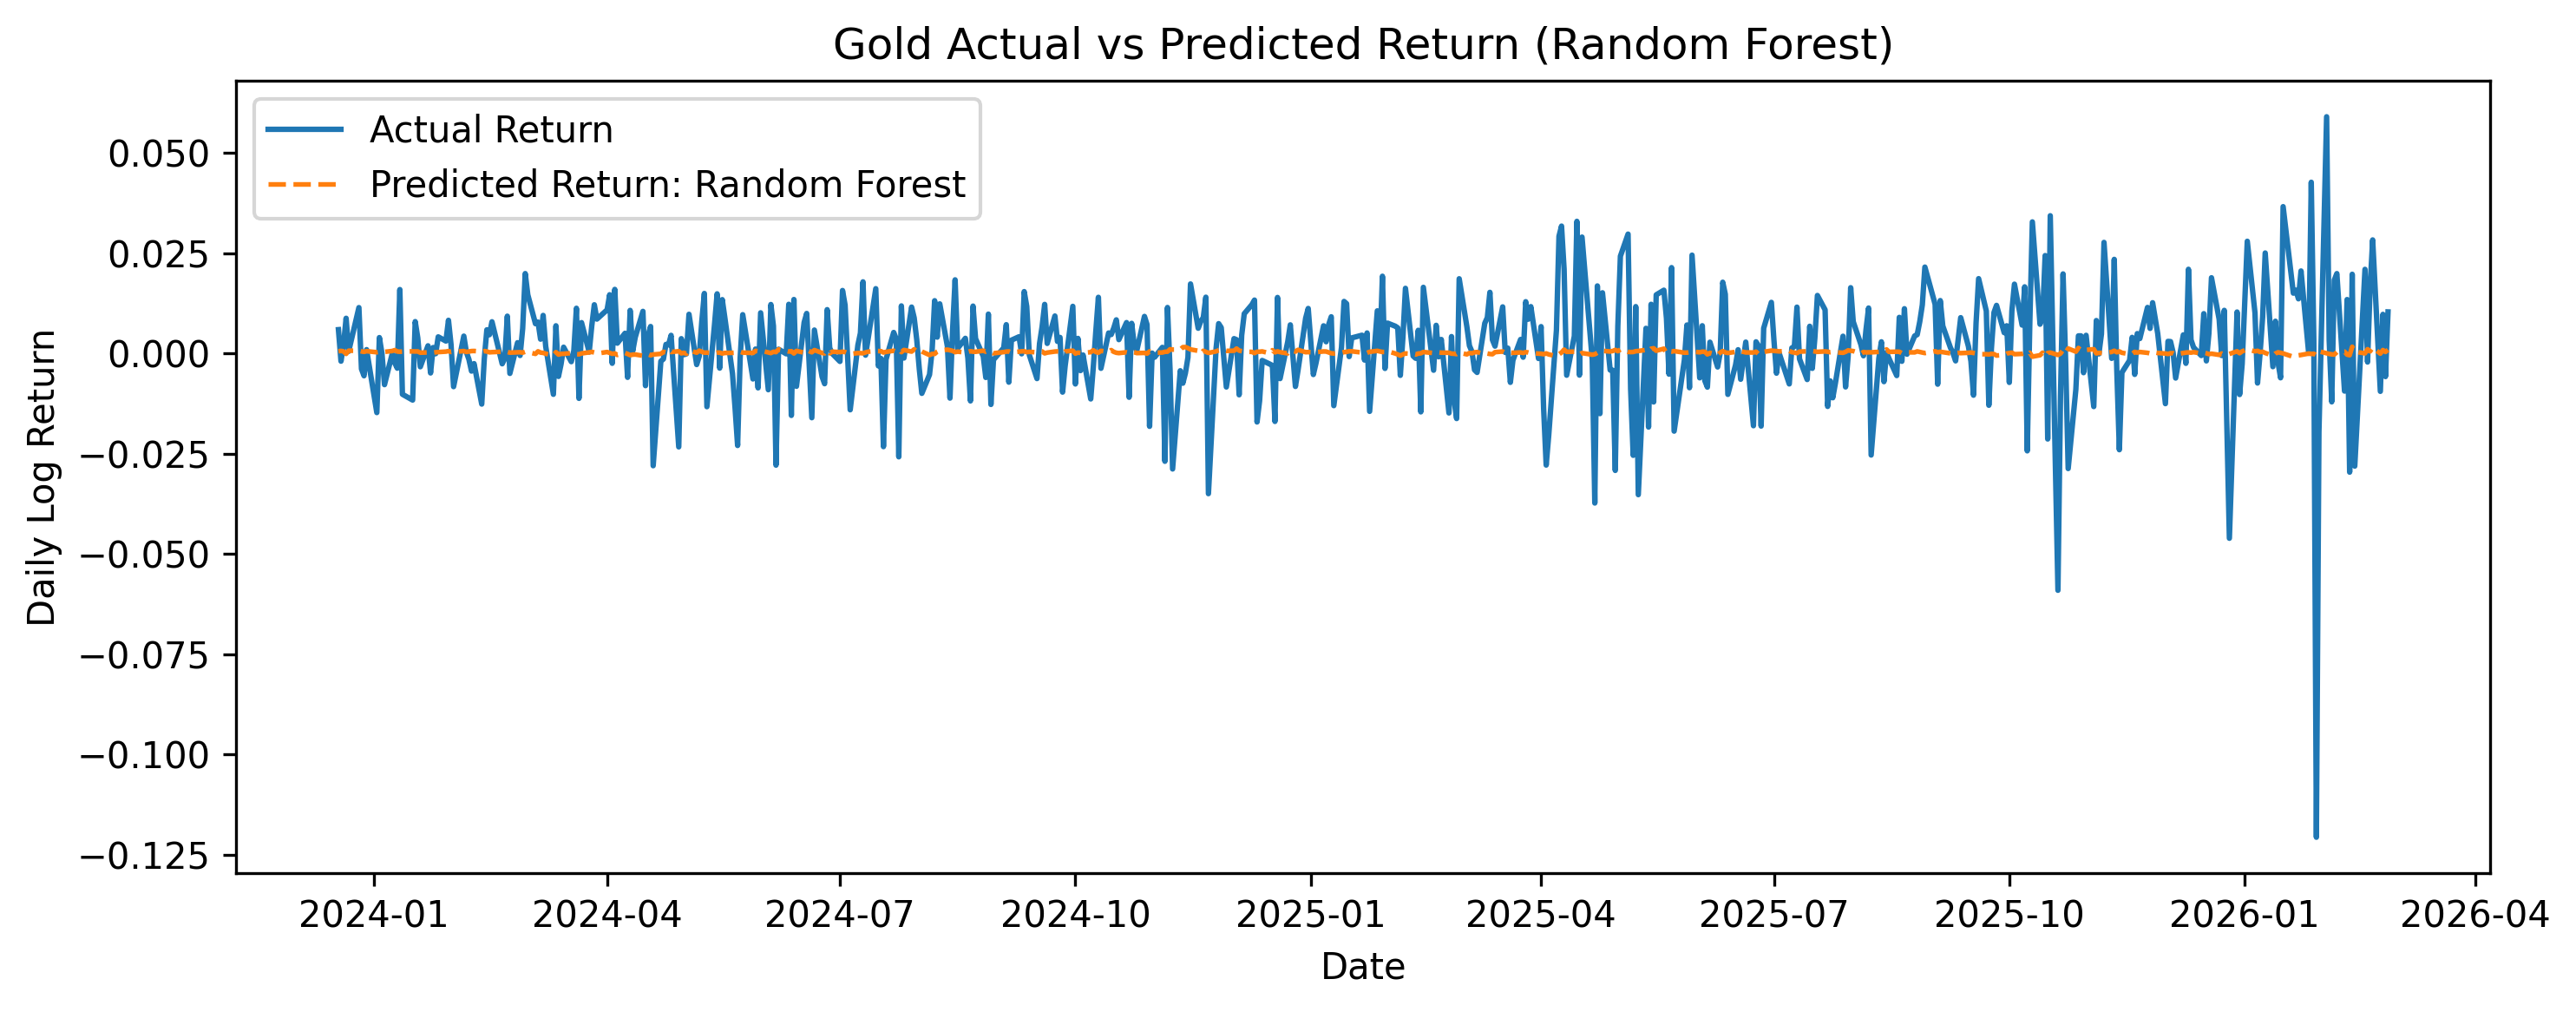
\includegraphics[width=\textwidth, trim=0 6 0 6, clip]{modeling_return_plot/Gold_Random_Forest_return_prediction.png}
        \caption{Gold -- RF}
    \end{subfigure}
    \hspace{0.025\textwidth}
    \begin{subfigure}[t]{0.29\textwidth}
        \centering
        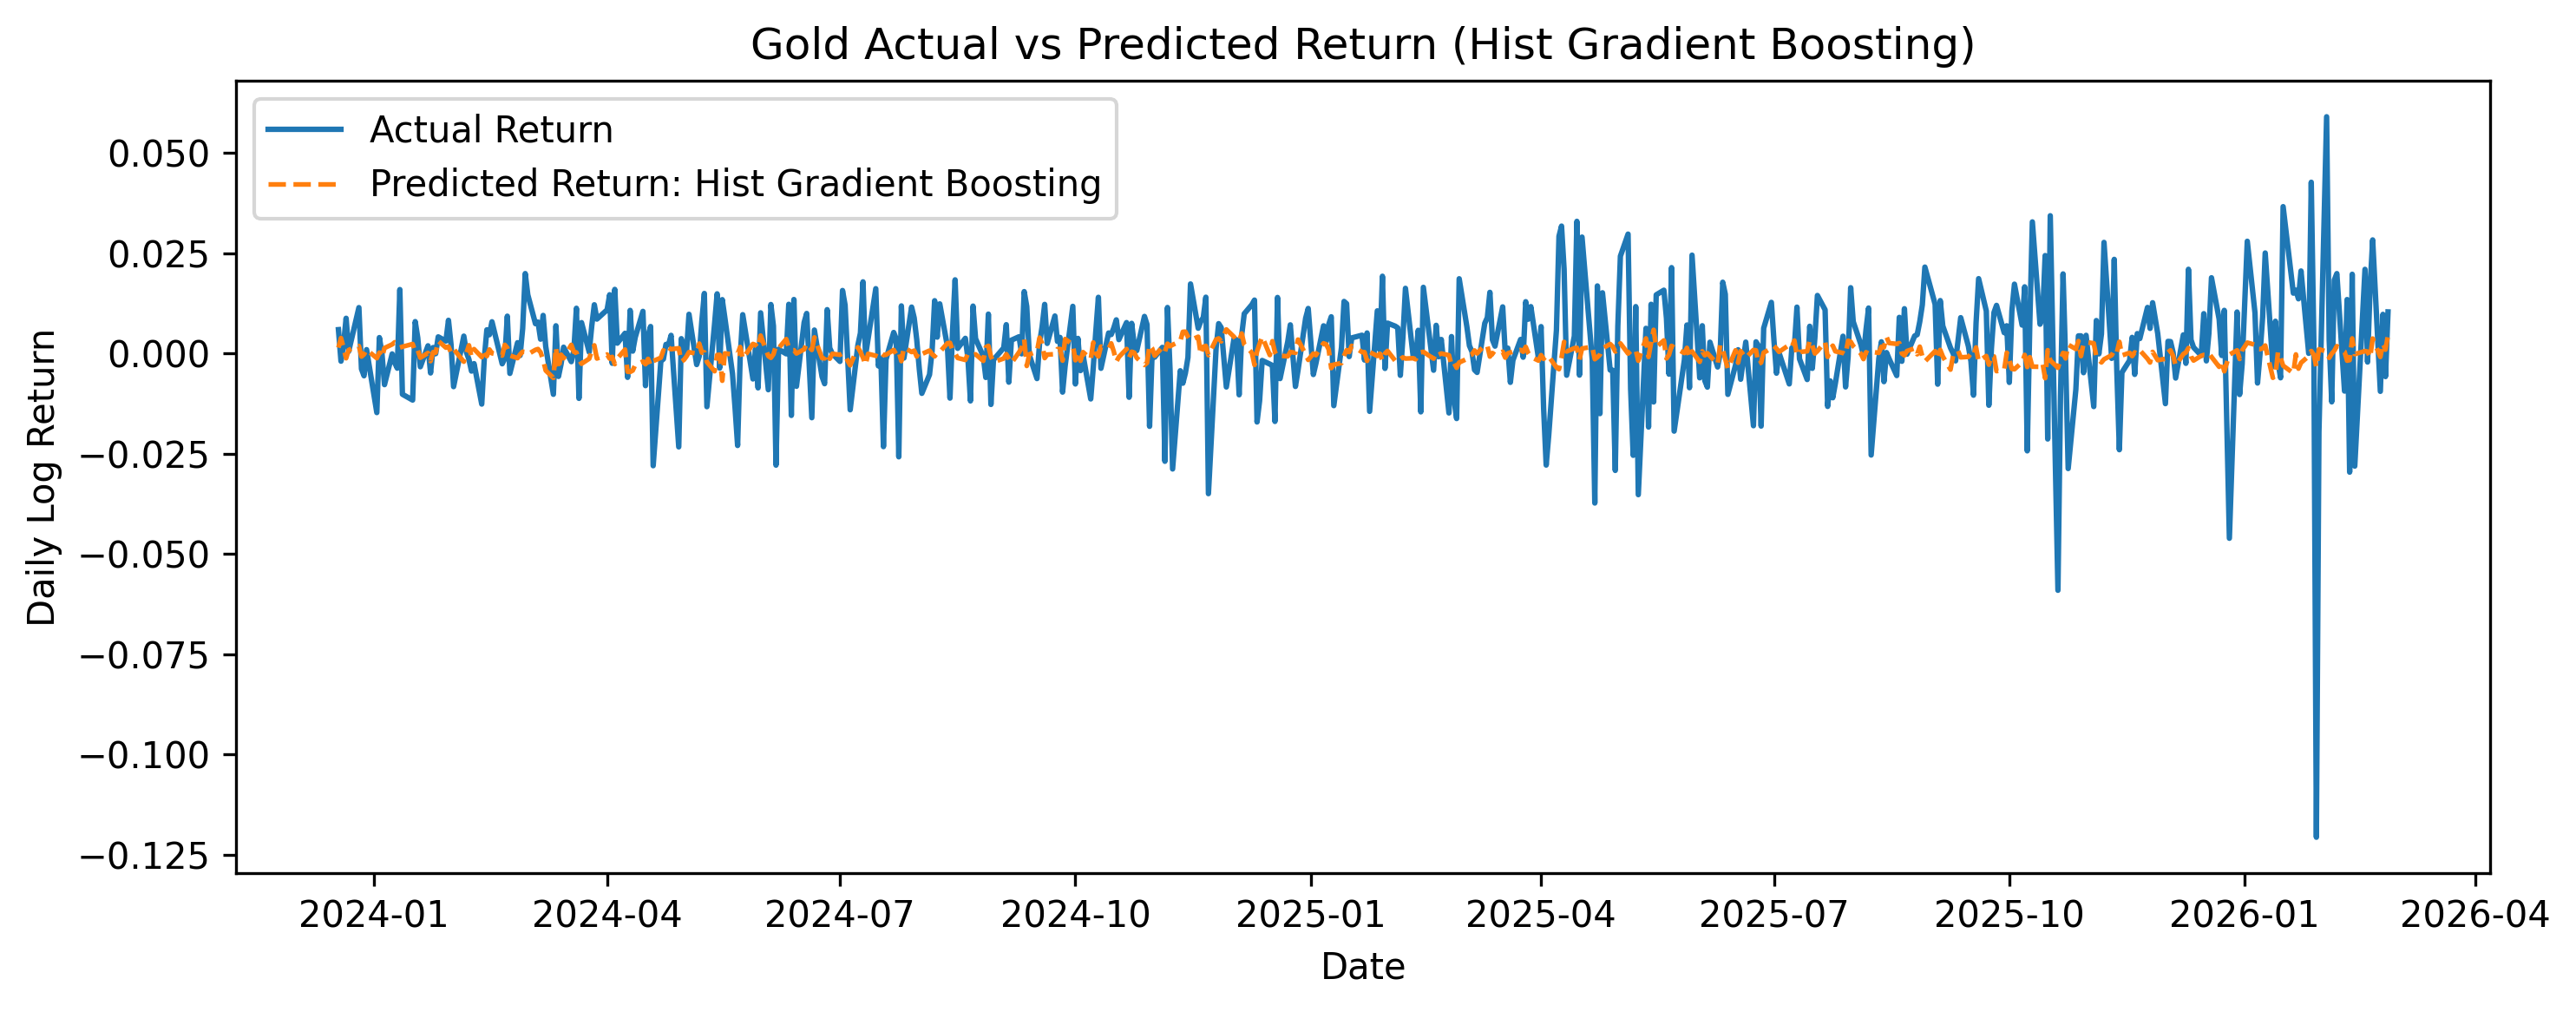
\includegraphics[width=\textwidth, trim=0 6 0 6, clip]{modeling_return_plot/Gold_Hist_Gradient_Boosting_return_prediction.png}
        \caption{Gold -- HGB}
    \end{subfigure}

    \vspace{0.20cm}

    % ---------------- Silver ----------------
    \begin{subfigure}[t]{0.29\textwidth}
        \centering
        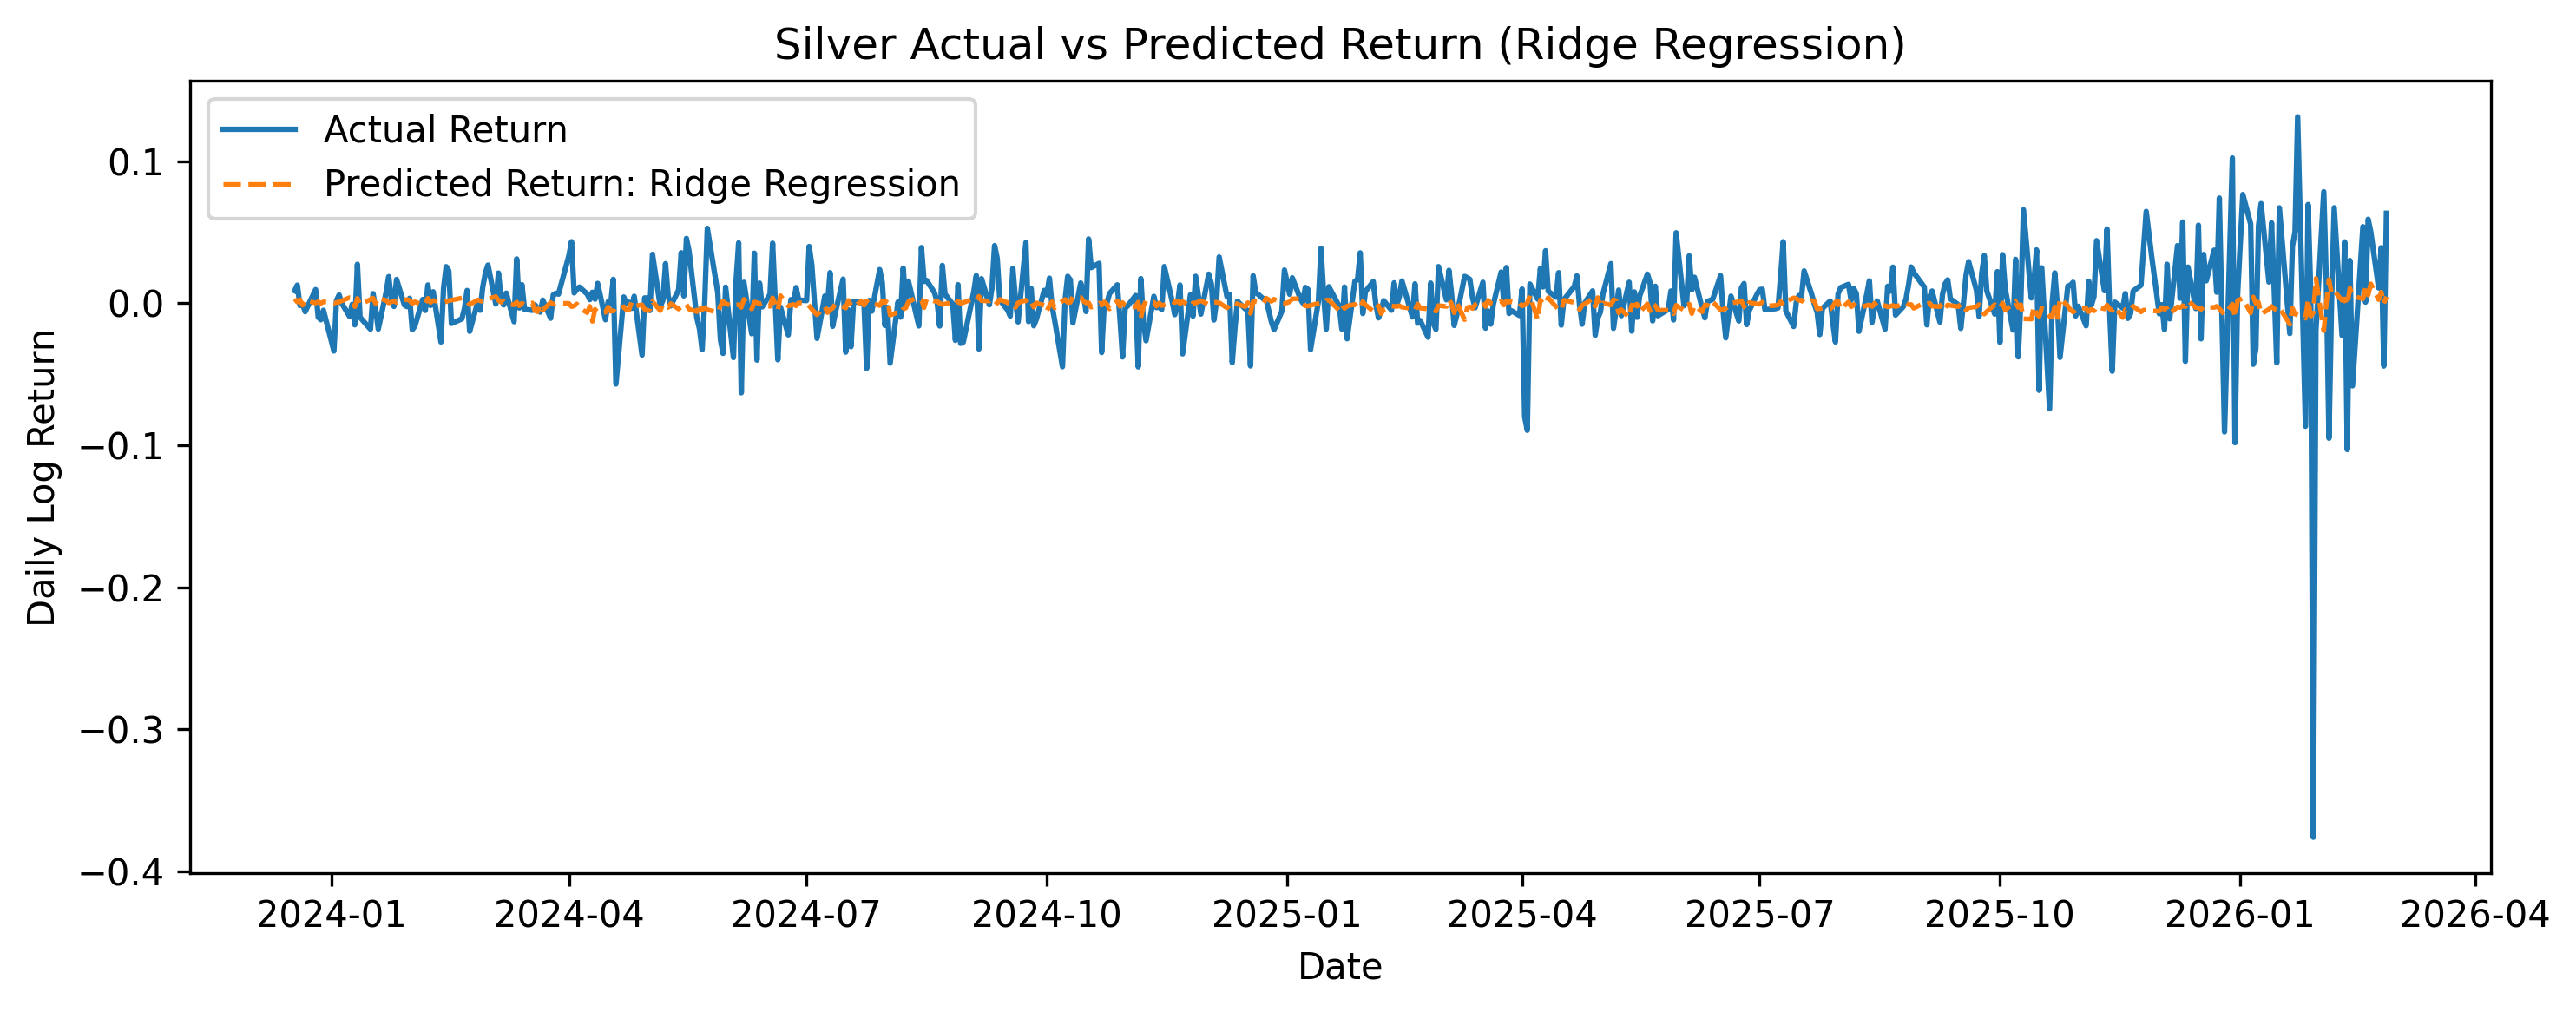
\includegraphics[width=\textwidth, trim=0 6 0 6, clip]{modeling_return_plot/Silver_Ridge_Regression_return_prediction.png}
        \caption{Silver -- Ridge}
    \end{subfigure}
    \hspace{0.025\textwidth}
    \begin{subfigure}[t]{0.29\textwidth}
        \centering
        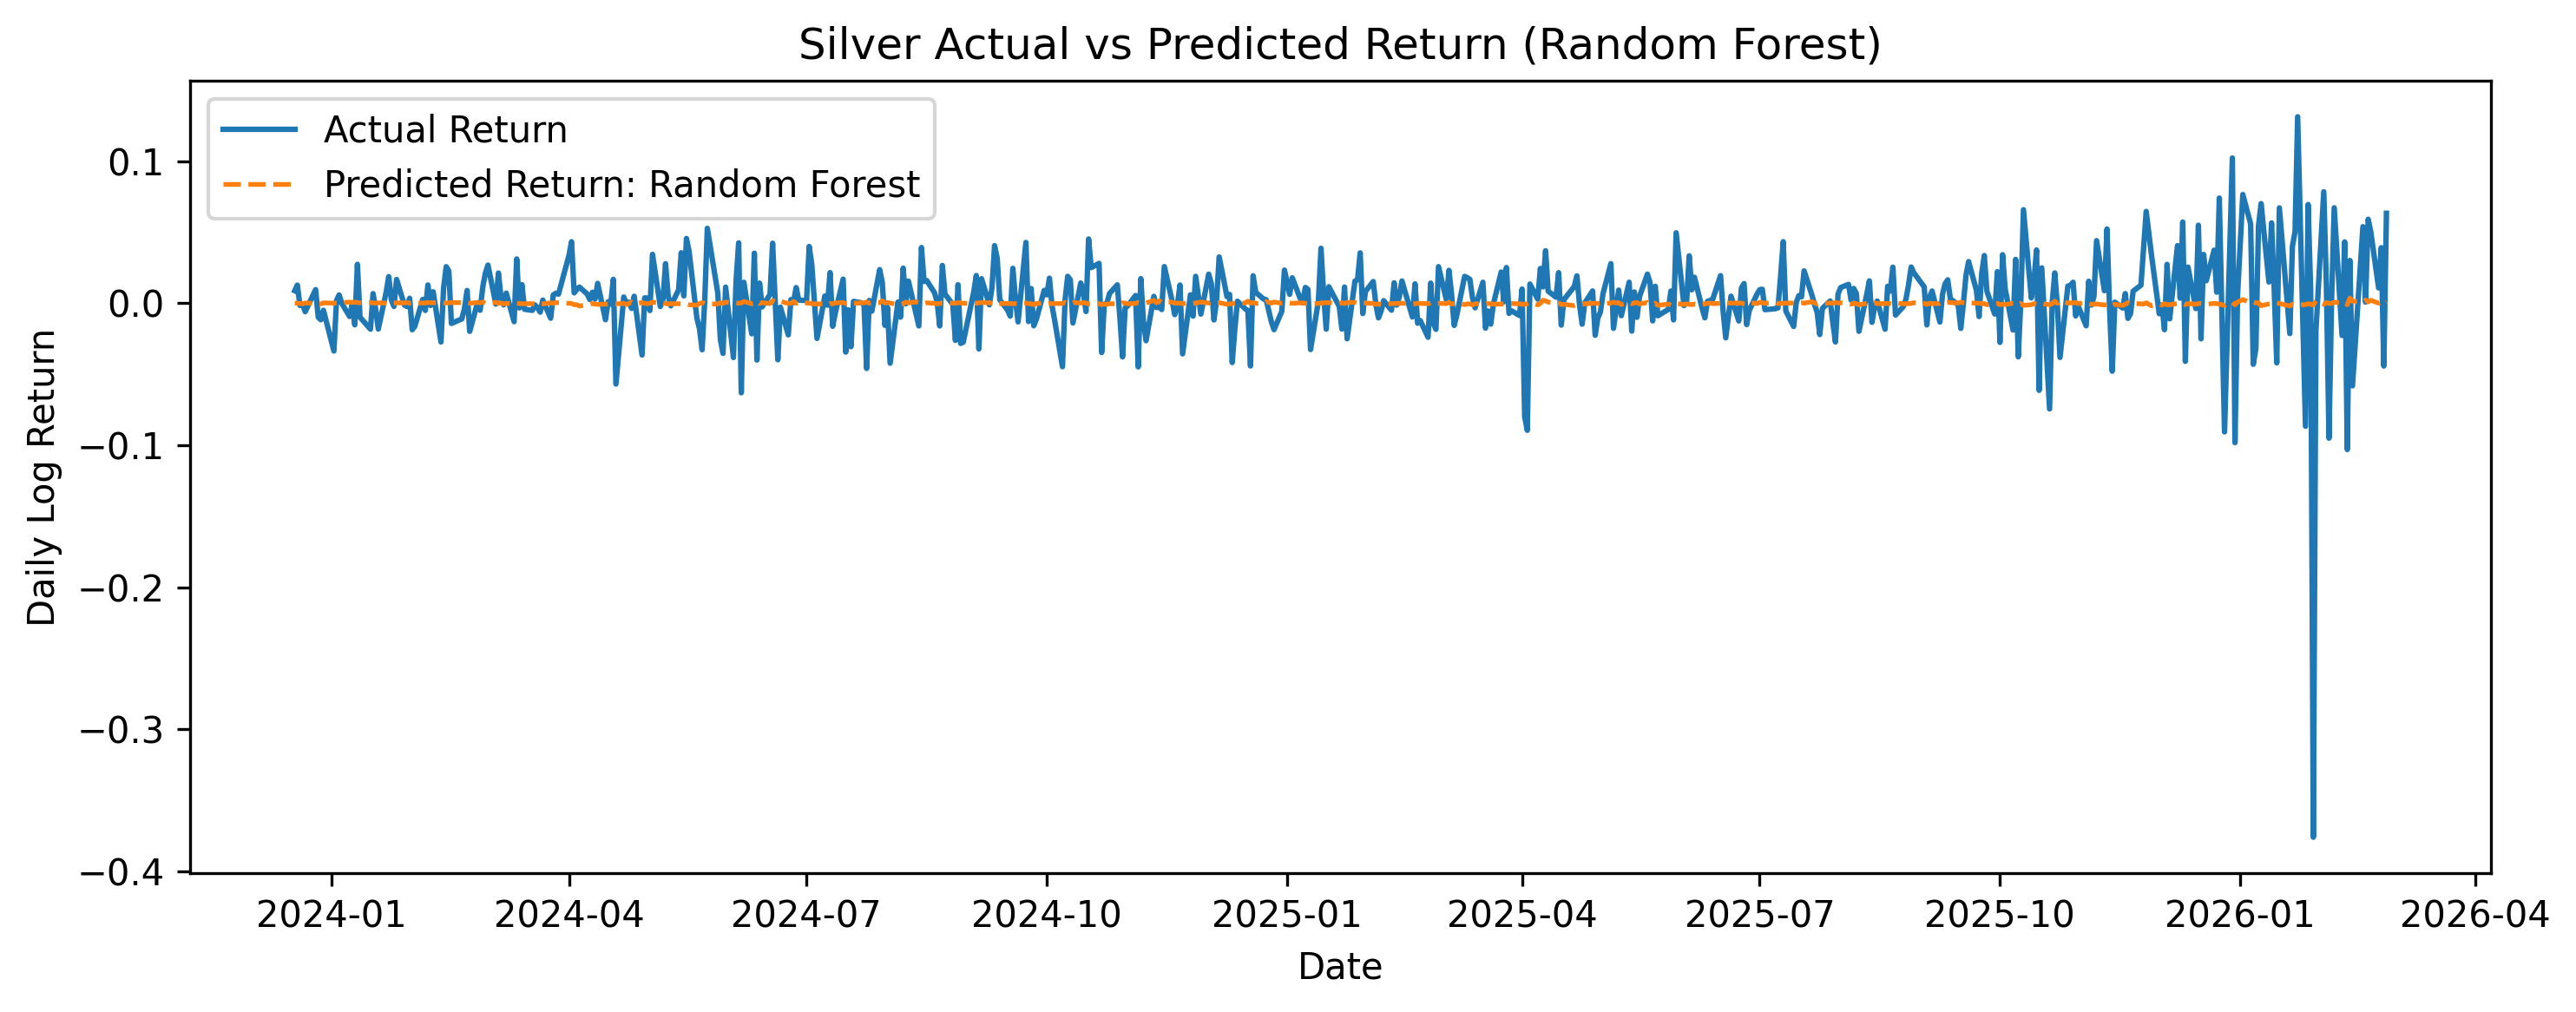
\includegraphics[width=\textwidth, trim=0 6 0 6, clip]{modeling_return_plot/Silver_Random_Forest_return_prediction.png}
        \caption{Silver -- RF}
    \end{subfigure}
    \hspace{0.025\textwidth}
    \begin{subfigure}[t]{0.29\textwidth}
        \centering
        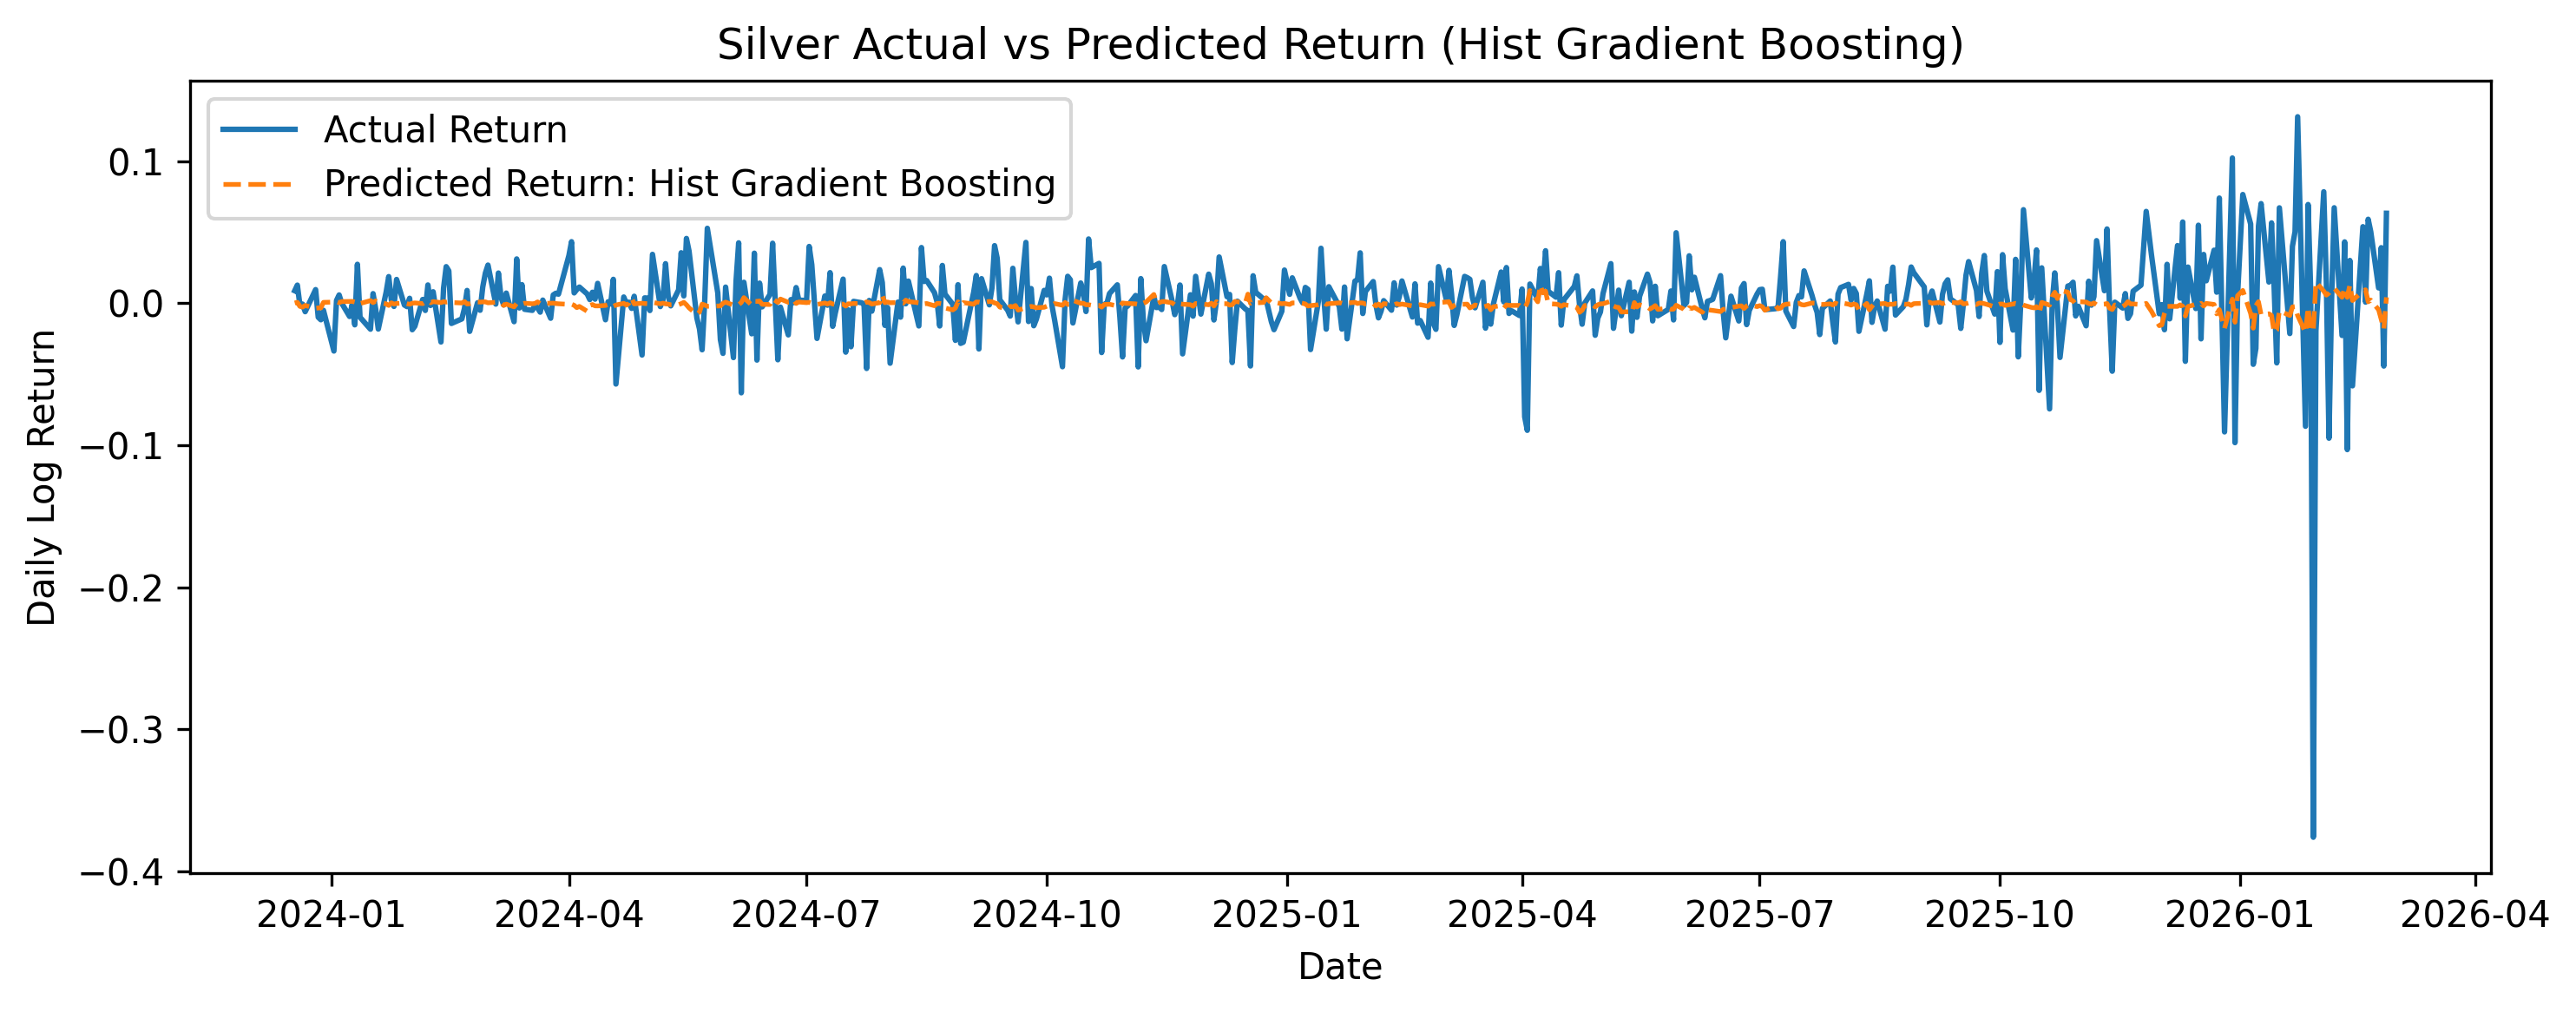
\includegraphics[width=\textwidth, trim=0 6 0 6, clip]{modeling_return_plot/Silver_Hist_Gradient_Boosting_return_prediction.png}
        \caption{Silver -- HGB}
    \end{subfigure}

    \vspace{0.12cm}
    \caption{Actual vs Predicted Returns for Precious Metals}
    \label{fig:return_predictions_metals}
\end{figure}

Figure~\ref{fig:return_predictions_metals} compares the actual and predicted next-day log returns for Gold and Silver. Since returns are much noisier than prices, the predicted series does not perfectly match every short-term spike. However, the plots still help evaluate whether the models capture the general return movement and volatility pattern of each asset.

% ------------------------------------------------------------
% Figure: Return Prediction Plots for USD Index and WTI Oil
% ------------------------------------------------------------

\begin{figure}[H]
    \centering
    \captionsetup[subfigure]{skip=4pt}
    \setlength{\abovecaptionskip}{5pt}
    \setlength{\belowcaptionskip}{3pt}

    % ---------------- USD Index ----------------
    \begin{subfigure}[t]{0.29\textwidth}
        \centering
        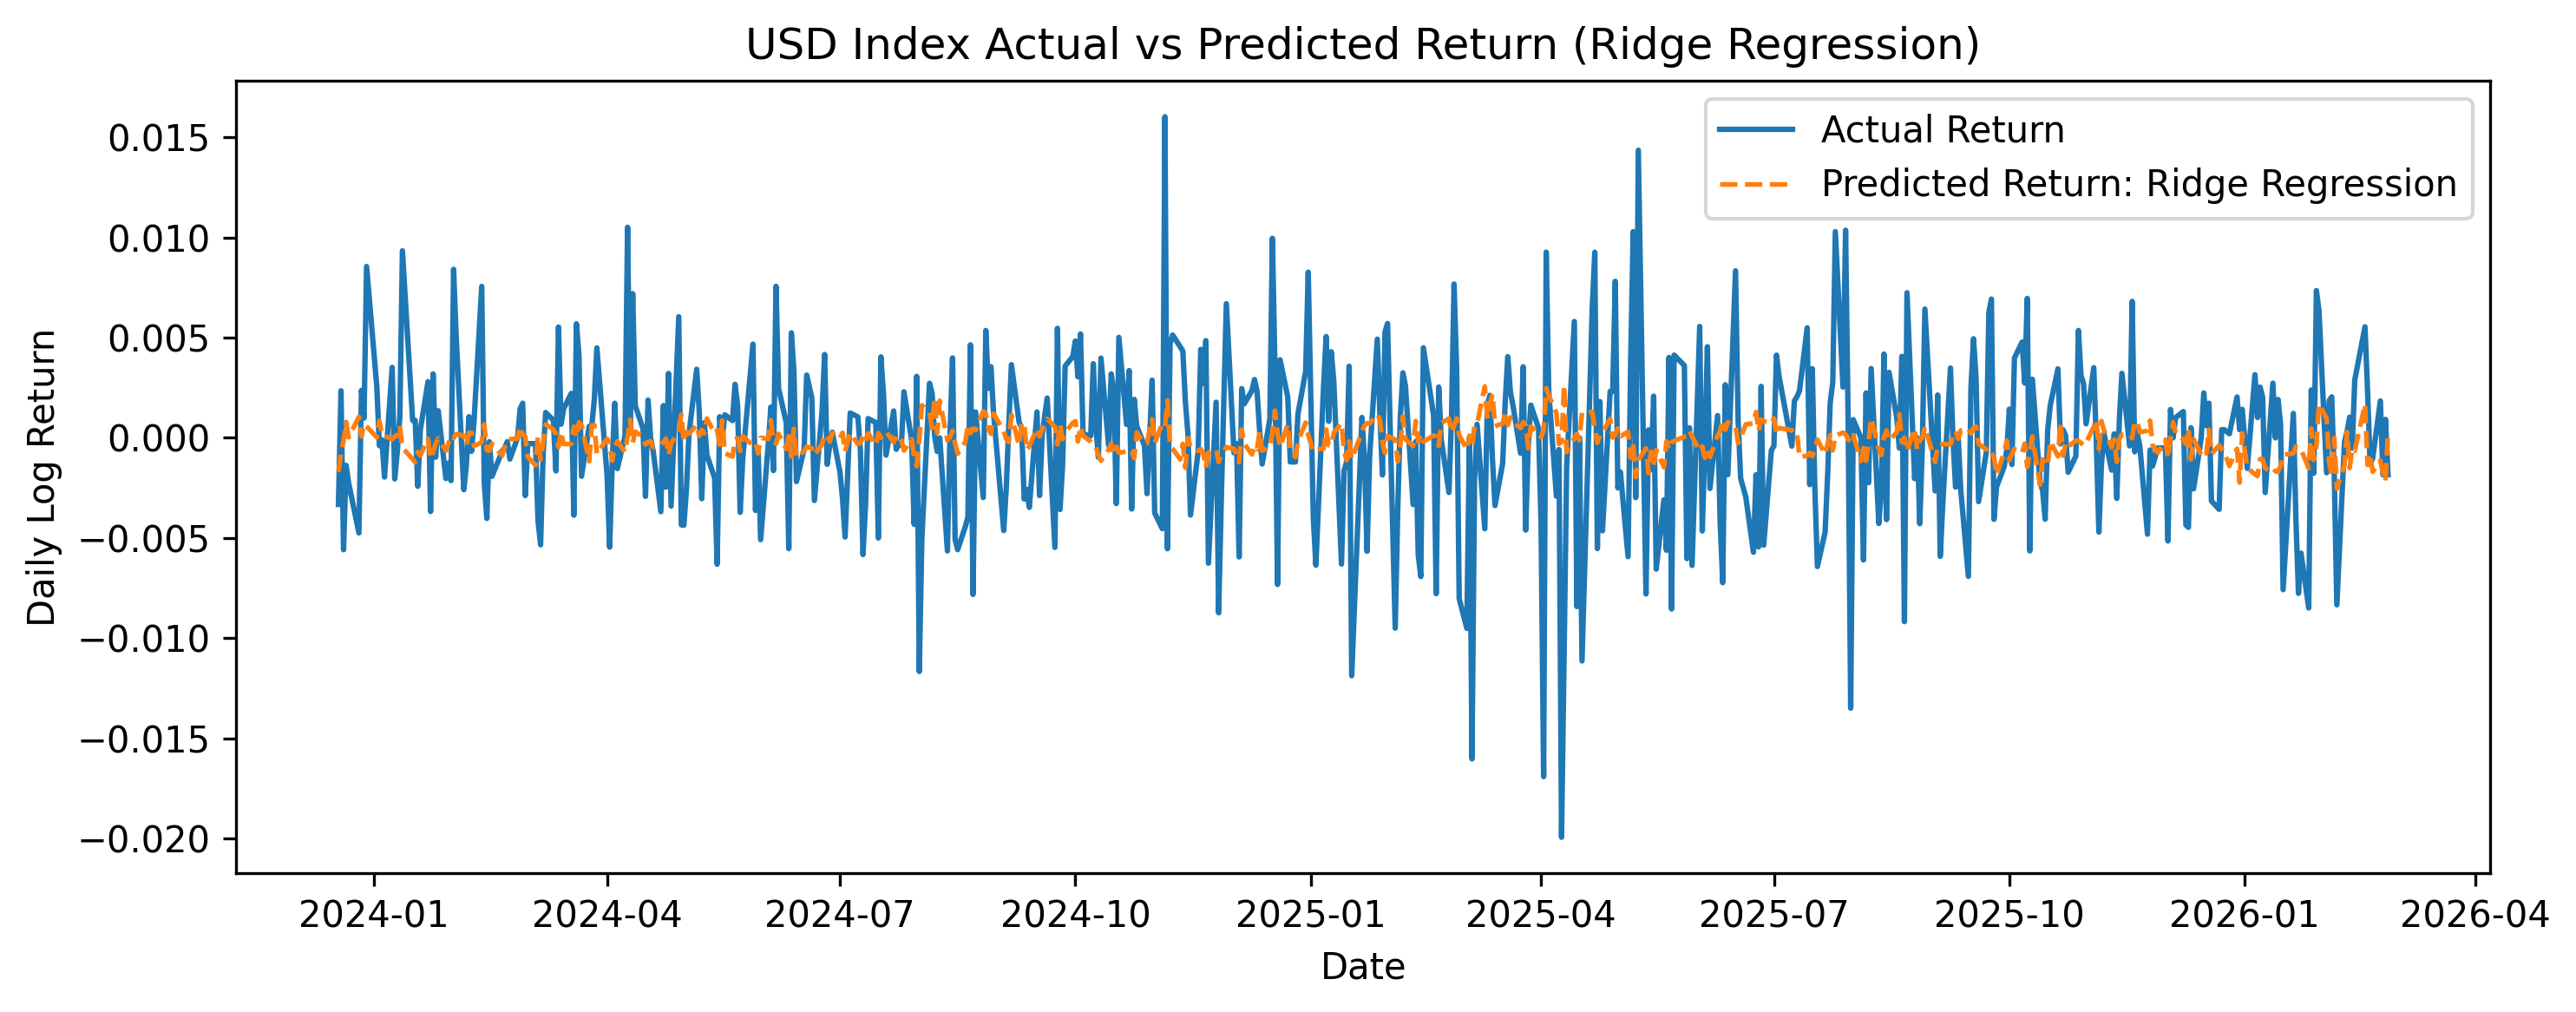
\includegraphics[width=\textwidth, trim=0 6 0 6, clip]{modeling_return_plot/USD_Index_Ridge_Regression_return_prediction.png}
        \caption{USD Index -- Ridge}
    \end{subfigure}
    \hspace{0.025\textwidth}
    \begin{subfigure}[t]{0.29\textwidth}
        \centering
        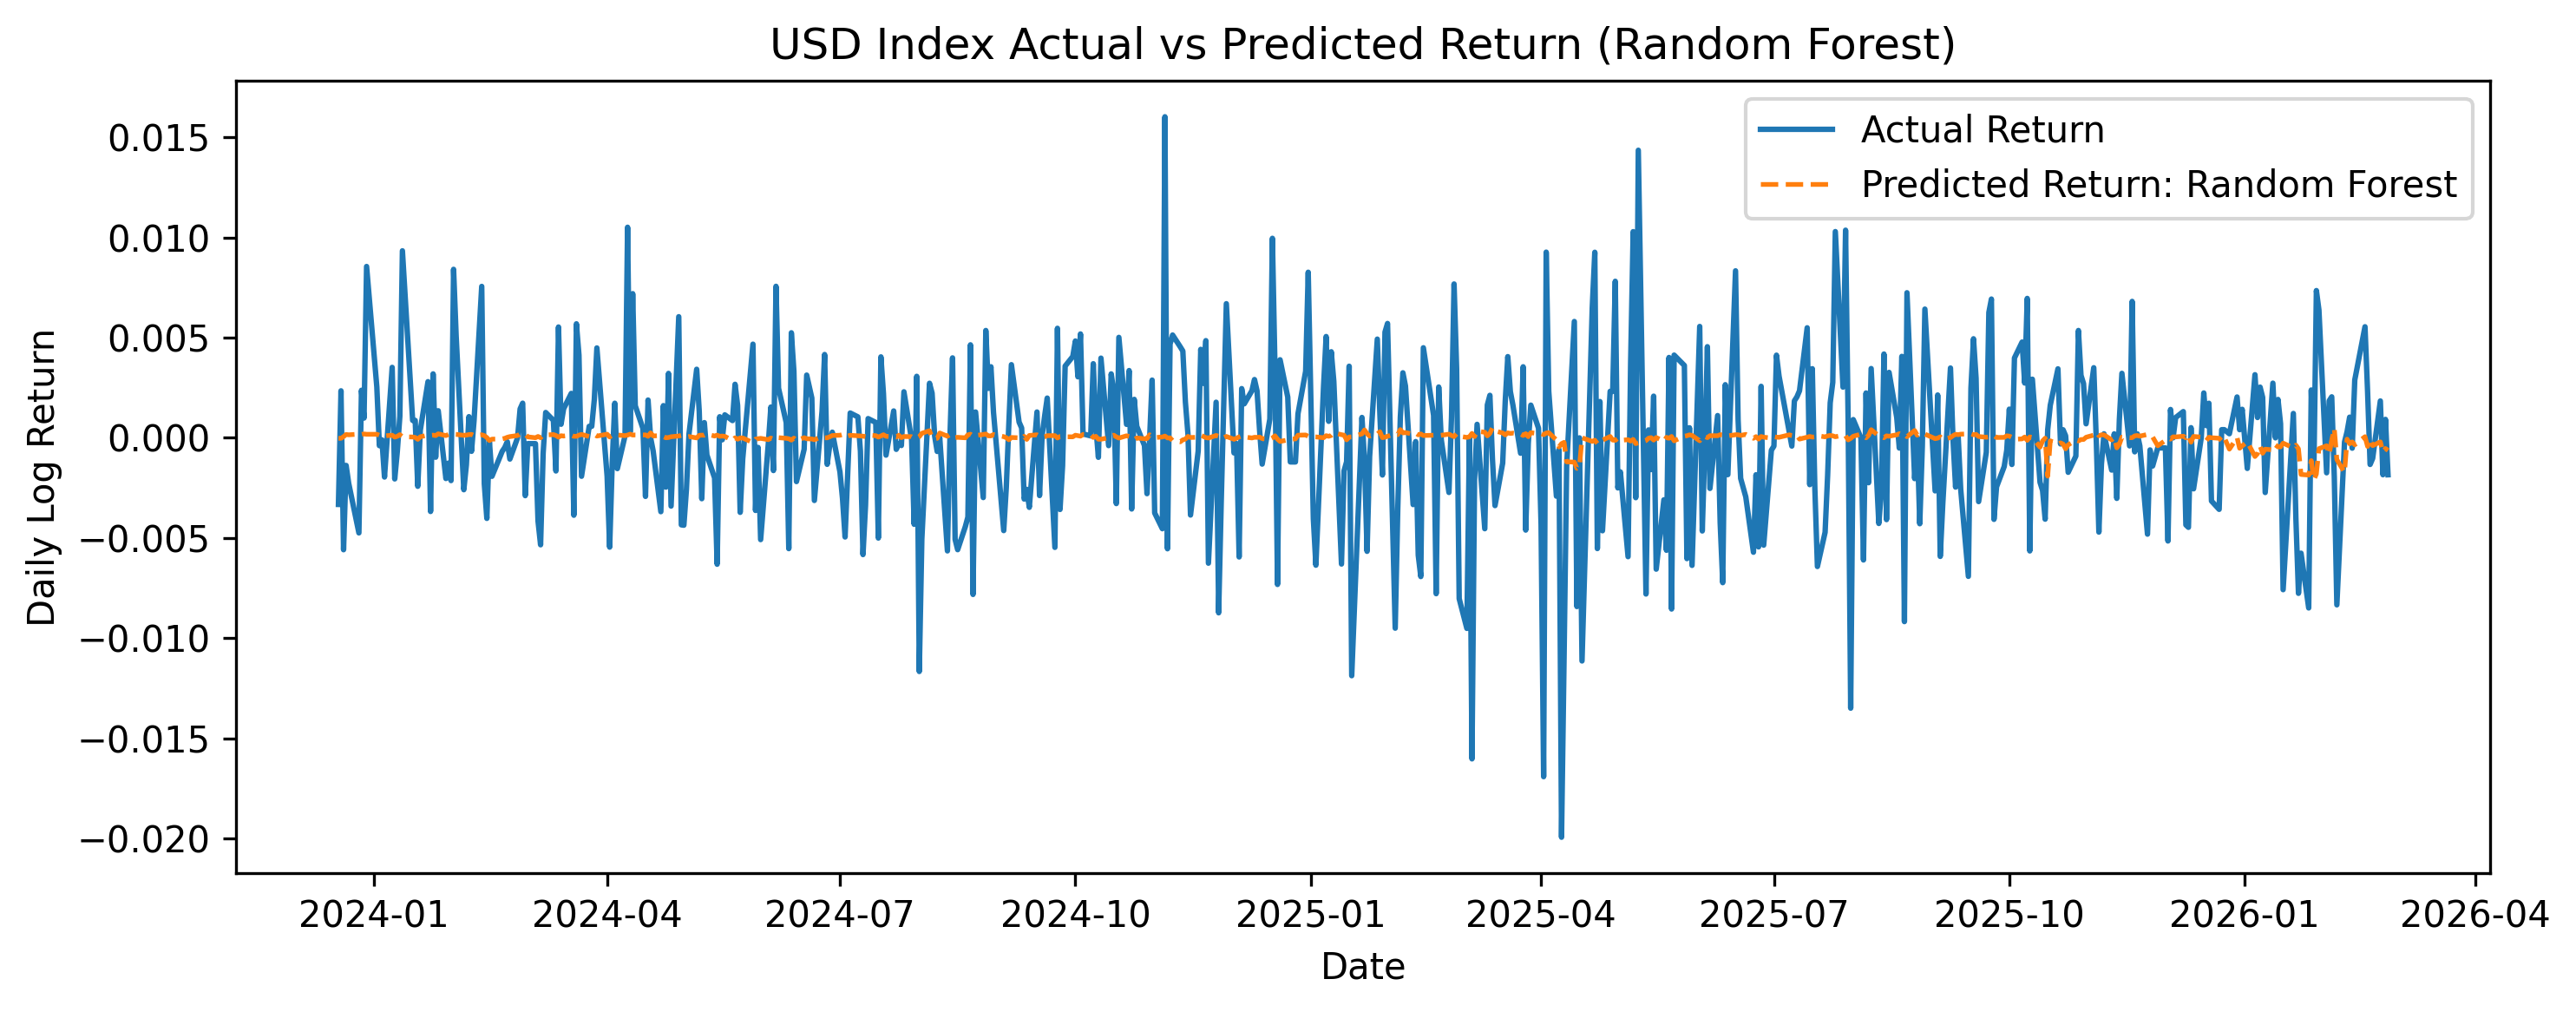
\includegraphics[width=\textwidth, trim=0 6 0 6, clip]{modeling_return_plot/USD_Index_Random_Forest_return_prediction.png}
        \caption{USD Index -- RF}
    \end{subfigure}
    \hspace{0.025\textwidth}
    \begin{subfigure}[t]{0.29\textwidth}
        \centering
        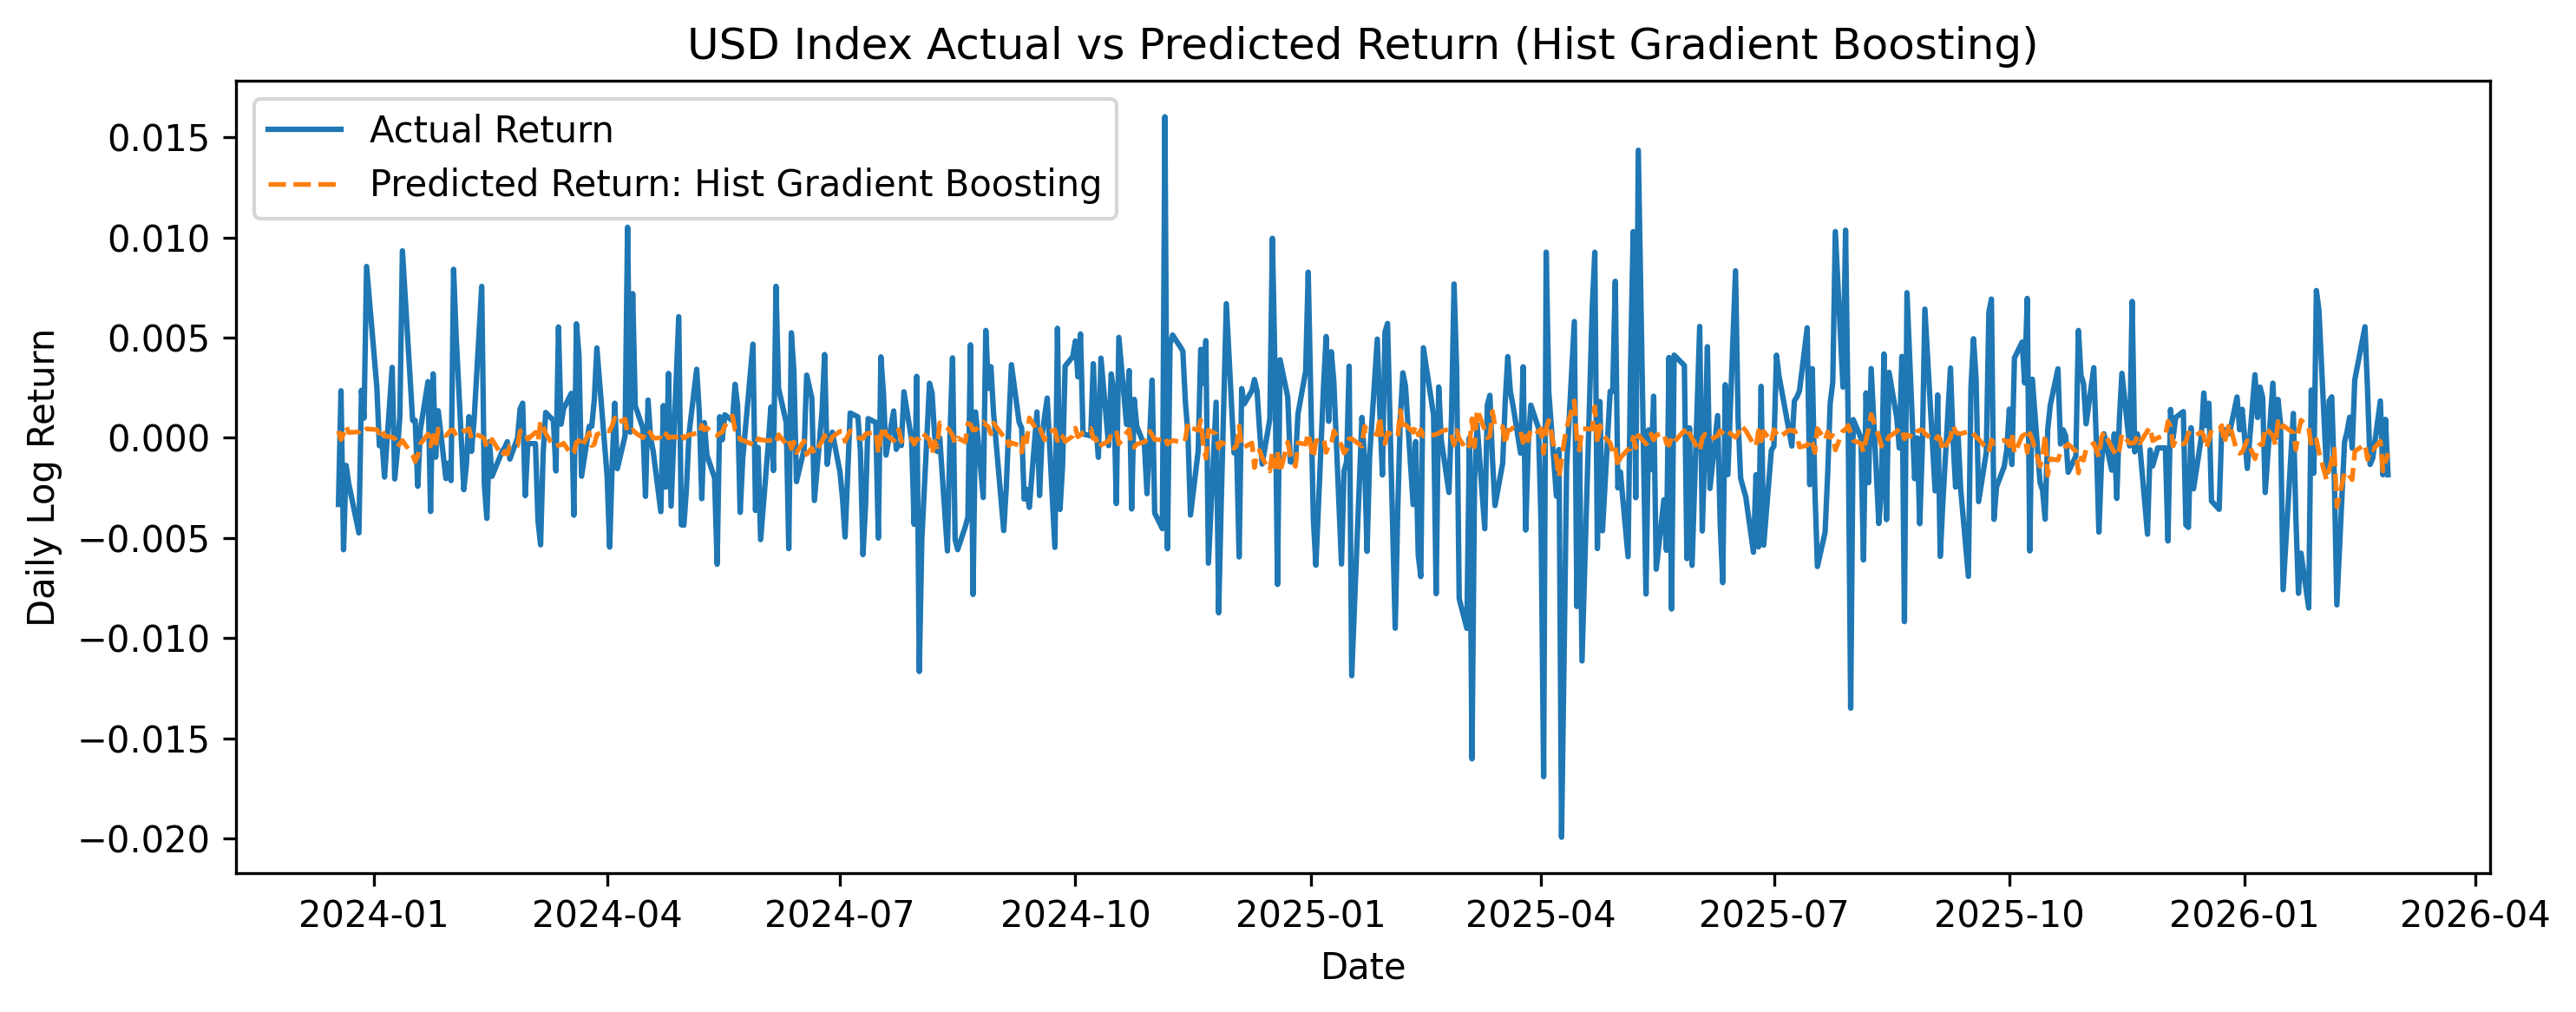
\includegraphics[width=\textwidth, trim=0 6 0 6, clip]{modeling_return_plot/USD_Index_Hist_Gradient_Boosting_return_prediction.png}
        \caption{USD Index -- HGB}
    \end{subfigure}

    \vspace{0.20cm}

    % ---------------- WTI Oil ----------------
    \begin{subfigure}[t]{0.29\textwidth}
        \centering
        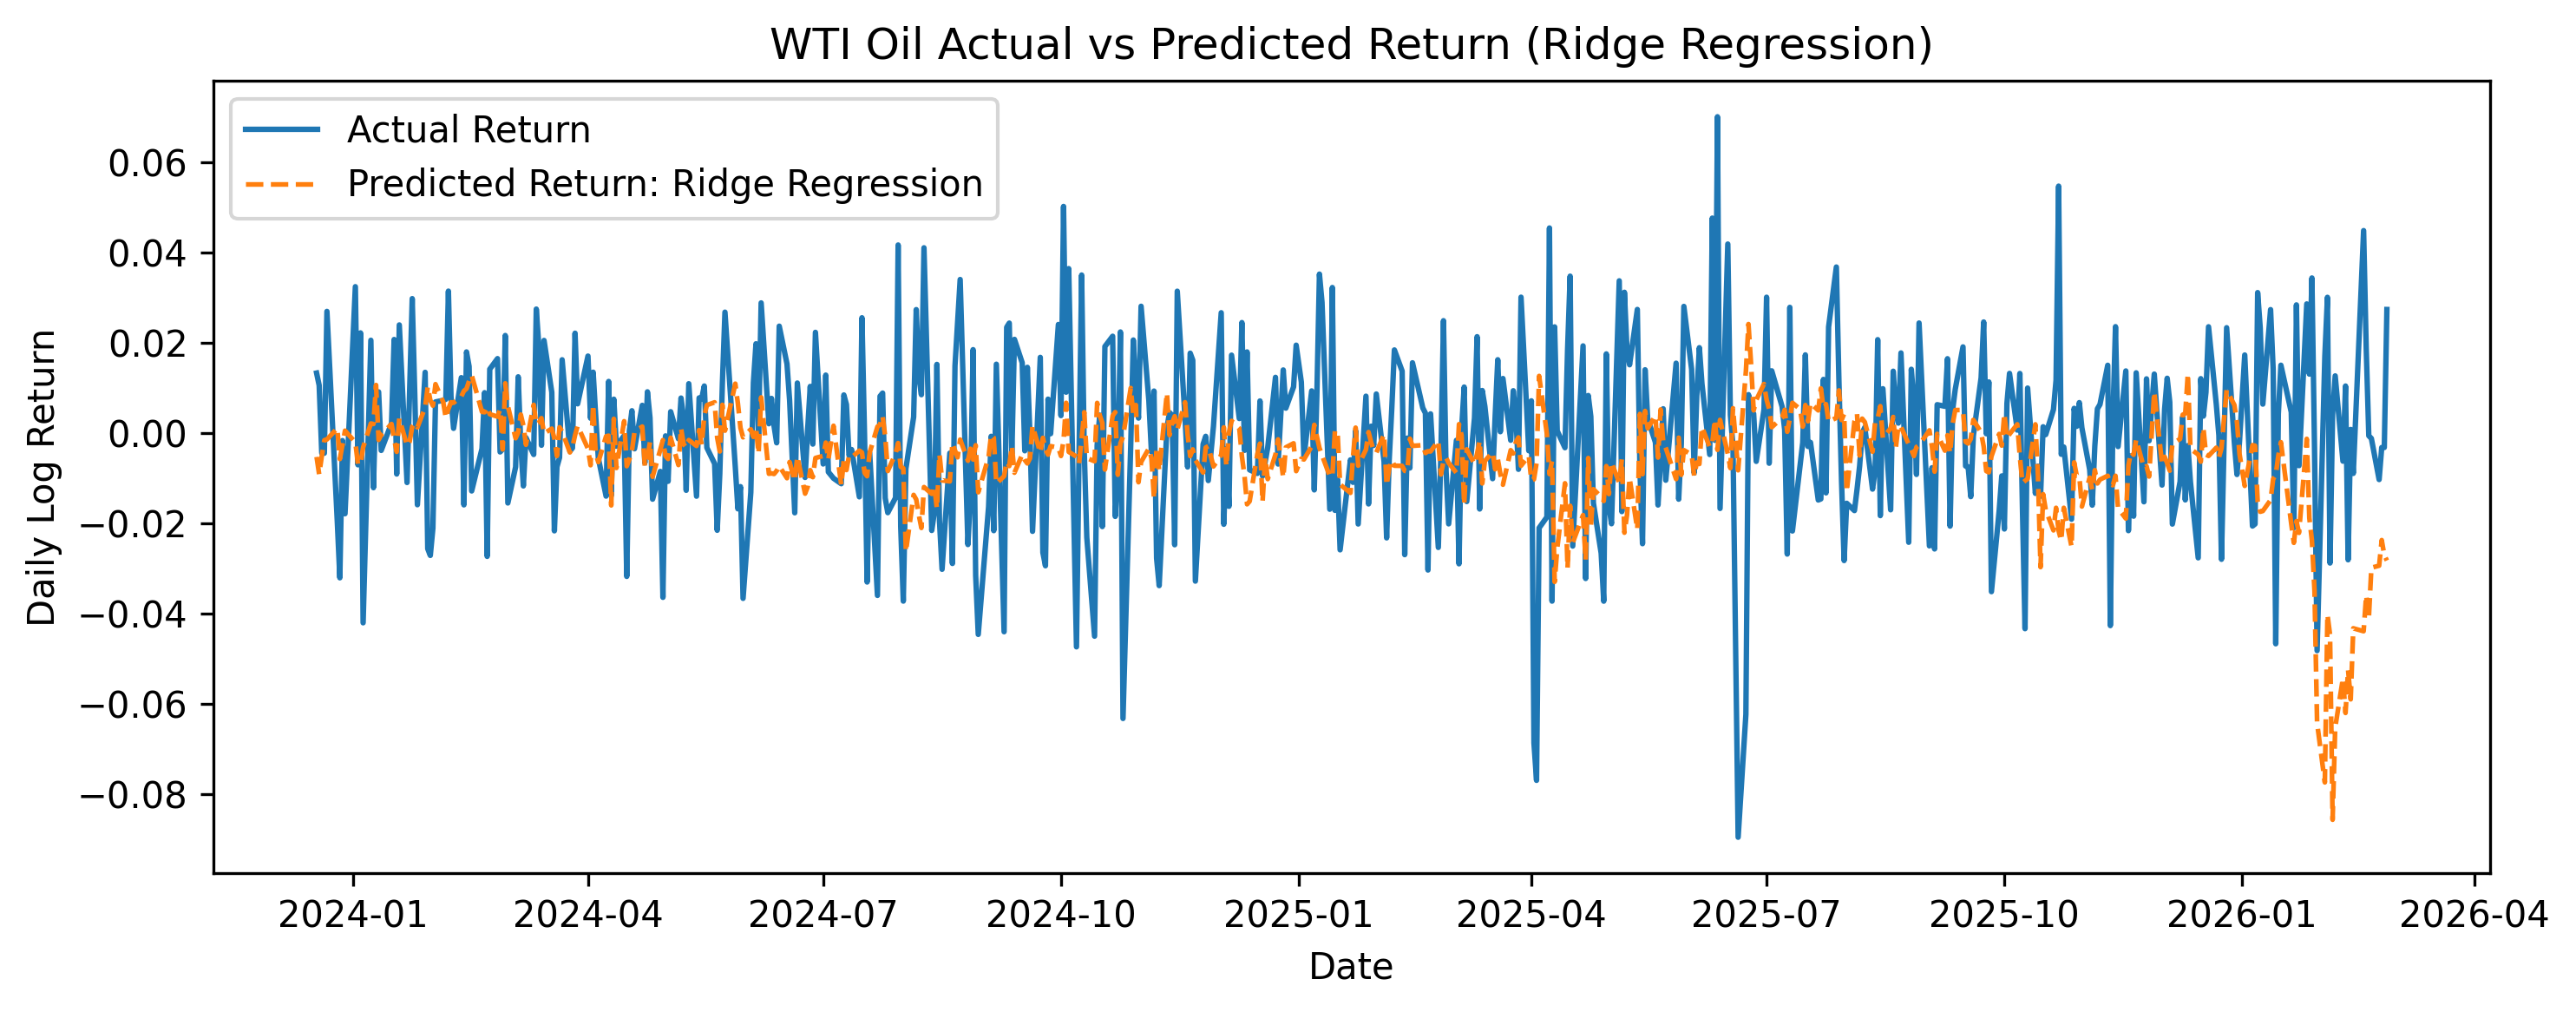
\includegraphics[width=\textwidth, trim=0 6 0 6, clip]{modeling_return_plot/WTI_Oil_Ridge_Regression_return_prediction.png}
        \caption{WTI Oil -- Ridge}
    \end{subfigure}
    \hspace{0.025\textwidth}
    \begin{subfigure}[t]{0.29\textwidth}
        \centering
        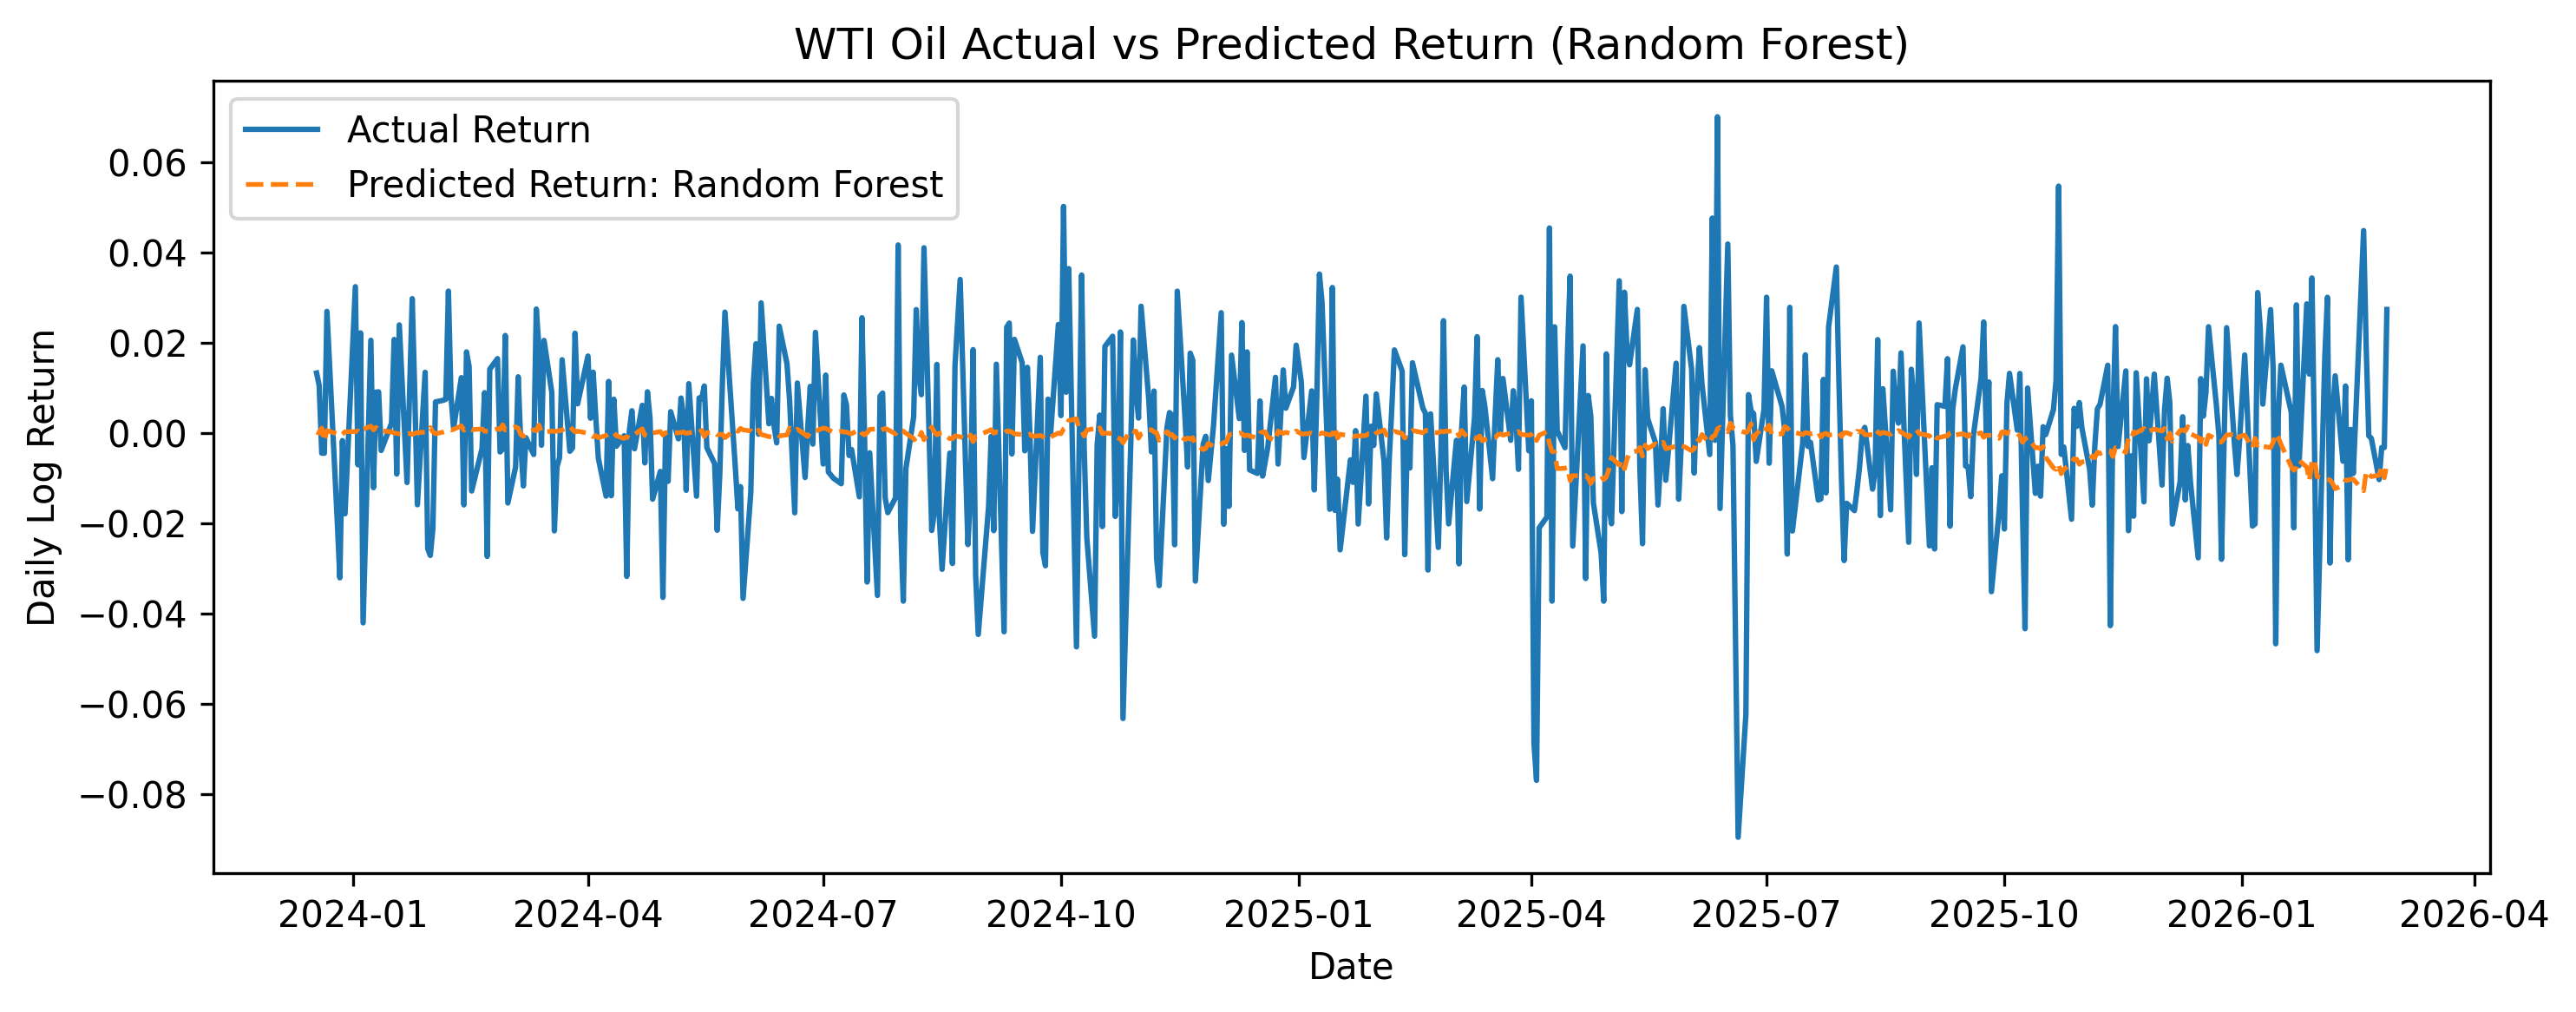
\includegraphics[width=\textwidth, trim=0 6 0 6, clip]{modeling_return_plot/WTI_Oil_Random_Forest_return_prediction.png}
        \caption{WTI Oil -- RF}
    \end{subfigure}
    \hspace{0.025\textwidth}
    \begin{subfigure}[t]{0.29\textwidth}
        \centering
        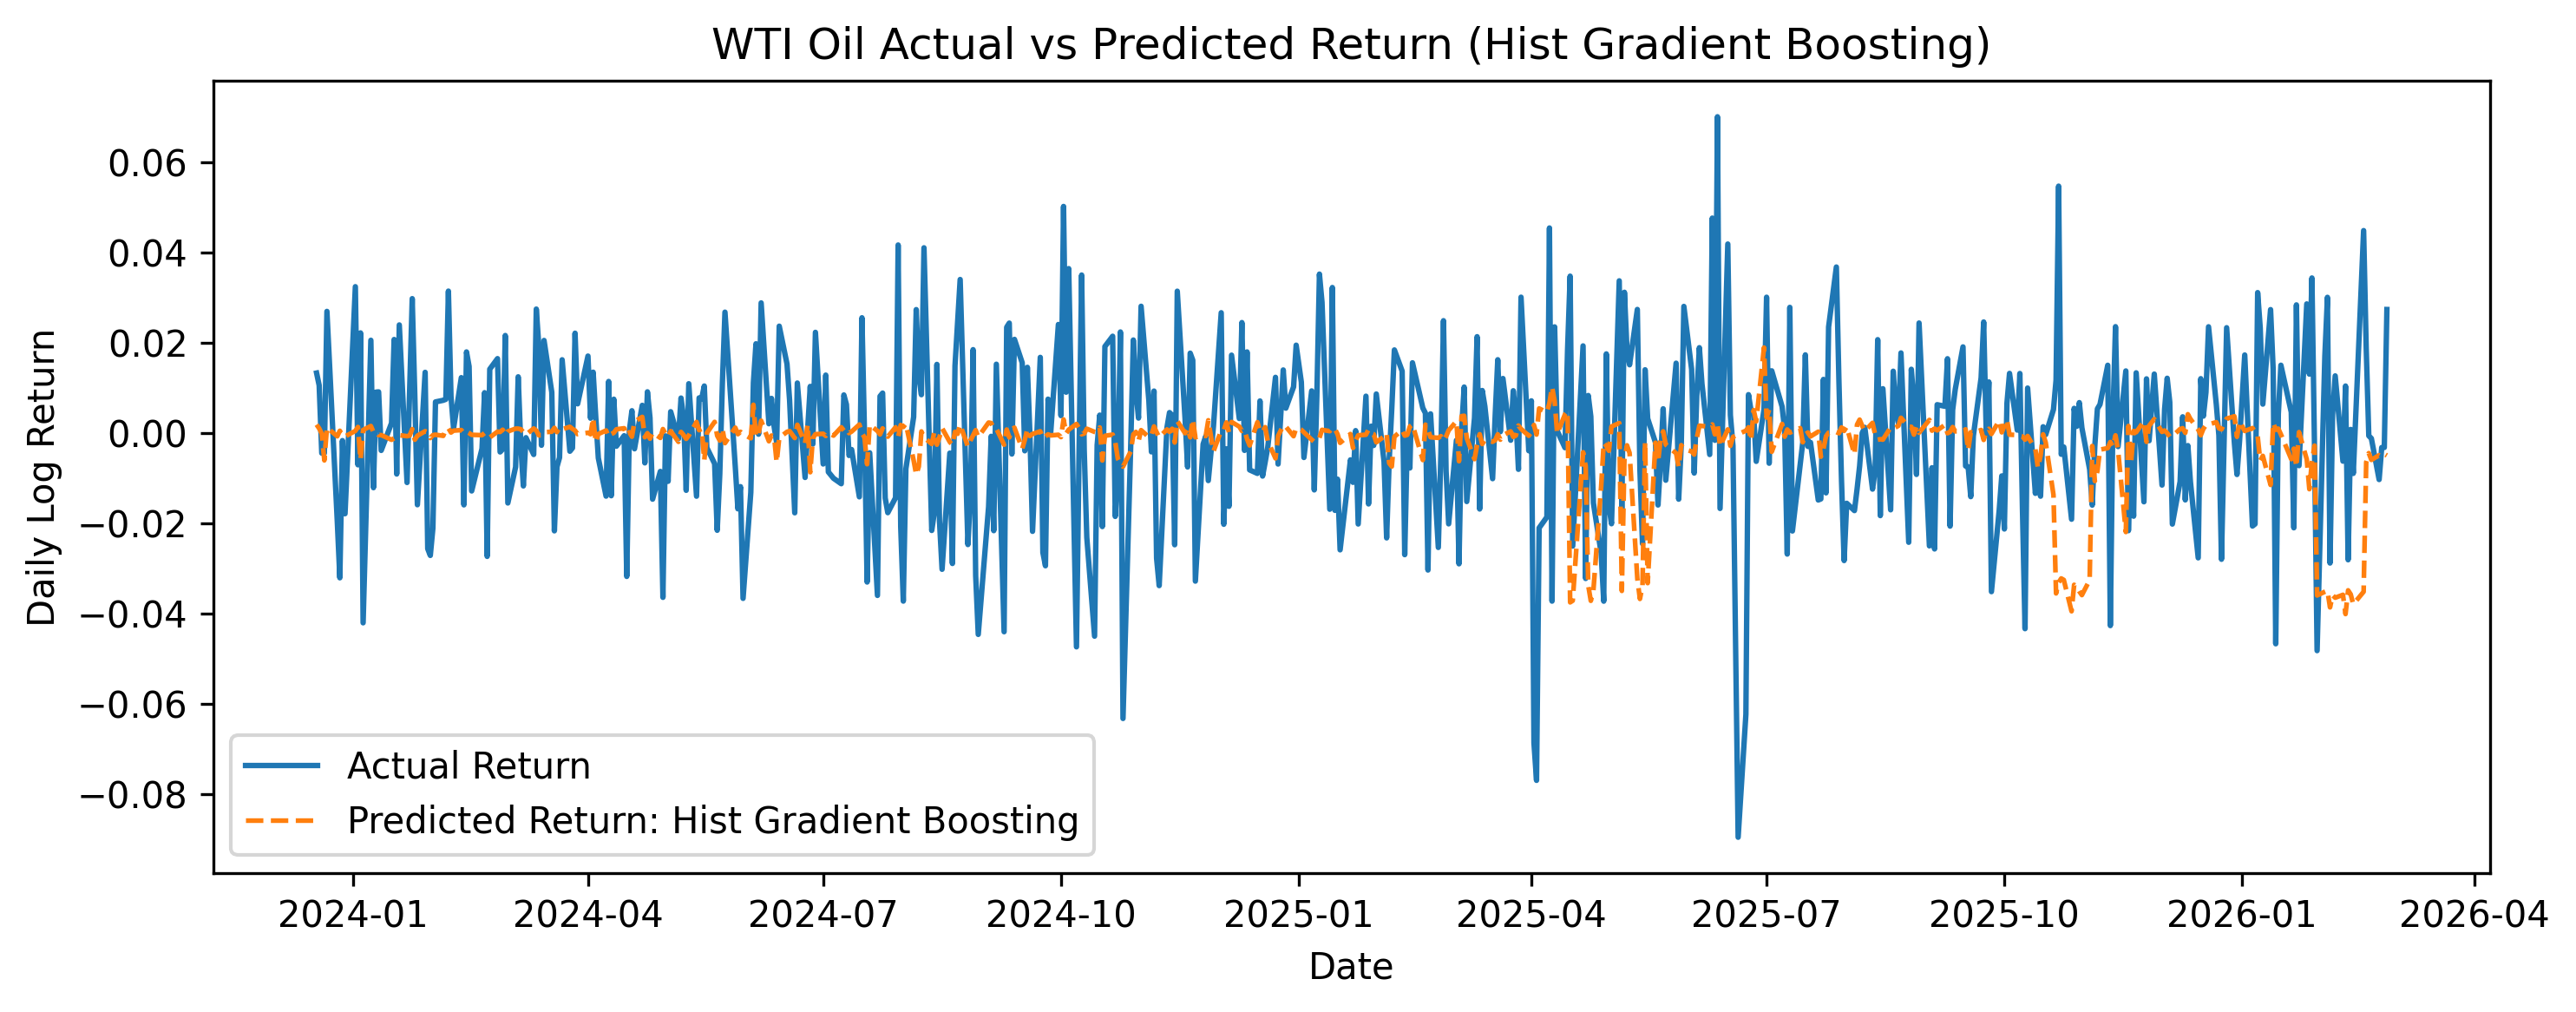
\includegraphics[width=\textwidth, trim=0 6 0 6, clip]{modeling_return_plot/WTI_Oil_Hist_Gradient_Boosting_return_prediction.png}
        \caption{WTI Oil -- HGB}
    \end{subfigure}

    \vspace{0.12cm}
    \caption{Actual vs Predicted Returns for USD Index and WTI Oil}
    \label{fig:return_predictions_macro}
\end{figure}

Figure~\ref{fig:return_predictions_macro} shows the return prediction results for USD Index and WTI Oil. The USD Index has relatively smaller return fluctuations, while WTI Oil shows larger shocks. This difference is useful because it shows that model performance should be interpreted together with each asset's volatility level.

% ------------------------------------------------------------
% Figure: Return Prediction Plots for Cryptocurrencies
% ------------------------------------------------------------

\begin{figure}[H]
    \centering
    \captionsetup[subfigure]{skip=4pt}
    \setlength{\abovecaptionskip}{5pt}
    \setlength{\belowcaptionskip}{3pt}

    % ---------------- Bitcoin ----------------
    \begin{subfigure}[t]{0.29\textwidth}
        \centering
        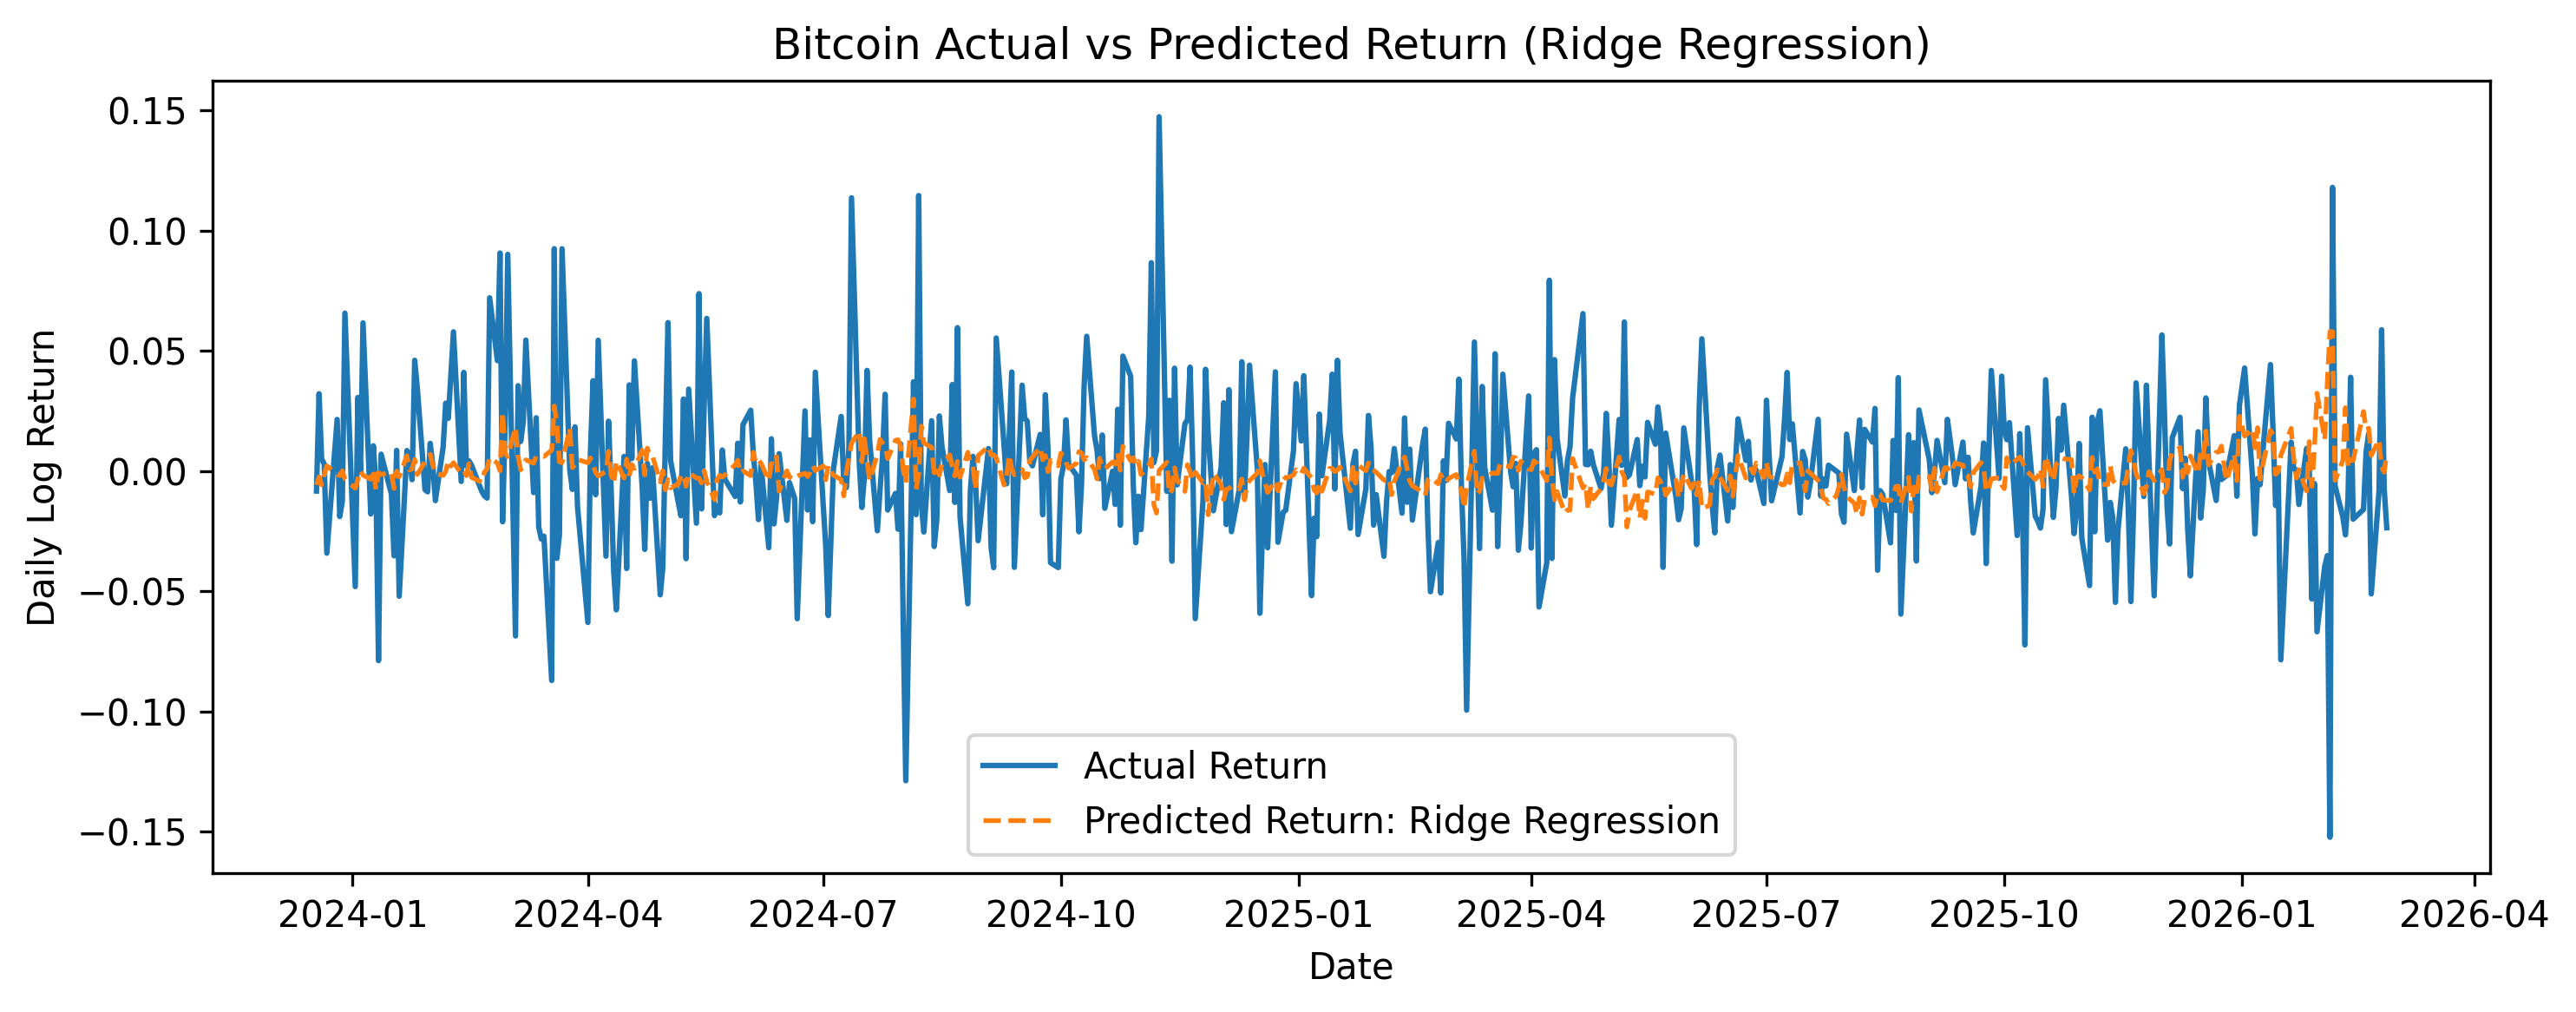
\includegraphics[width=\textwidth, trim=0 6 0 6, clip]{modeling_return_plot/Bitcoin_Ridge_Regression_return_prediction.png}
        \caption{Bitcoin -- Ridge}
    \end{subfigure}
    \hspace{0.025\textwidth}
    \begin{subfigure}[t]{0.29\textwidth}
        \centering
        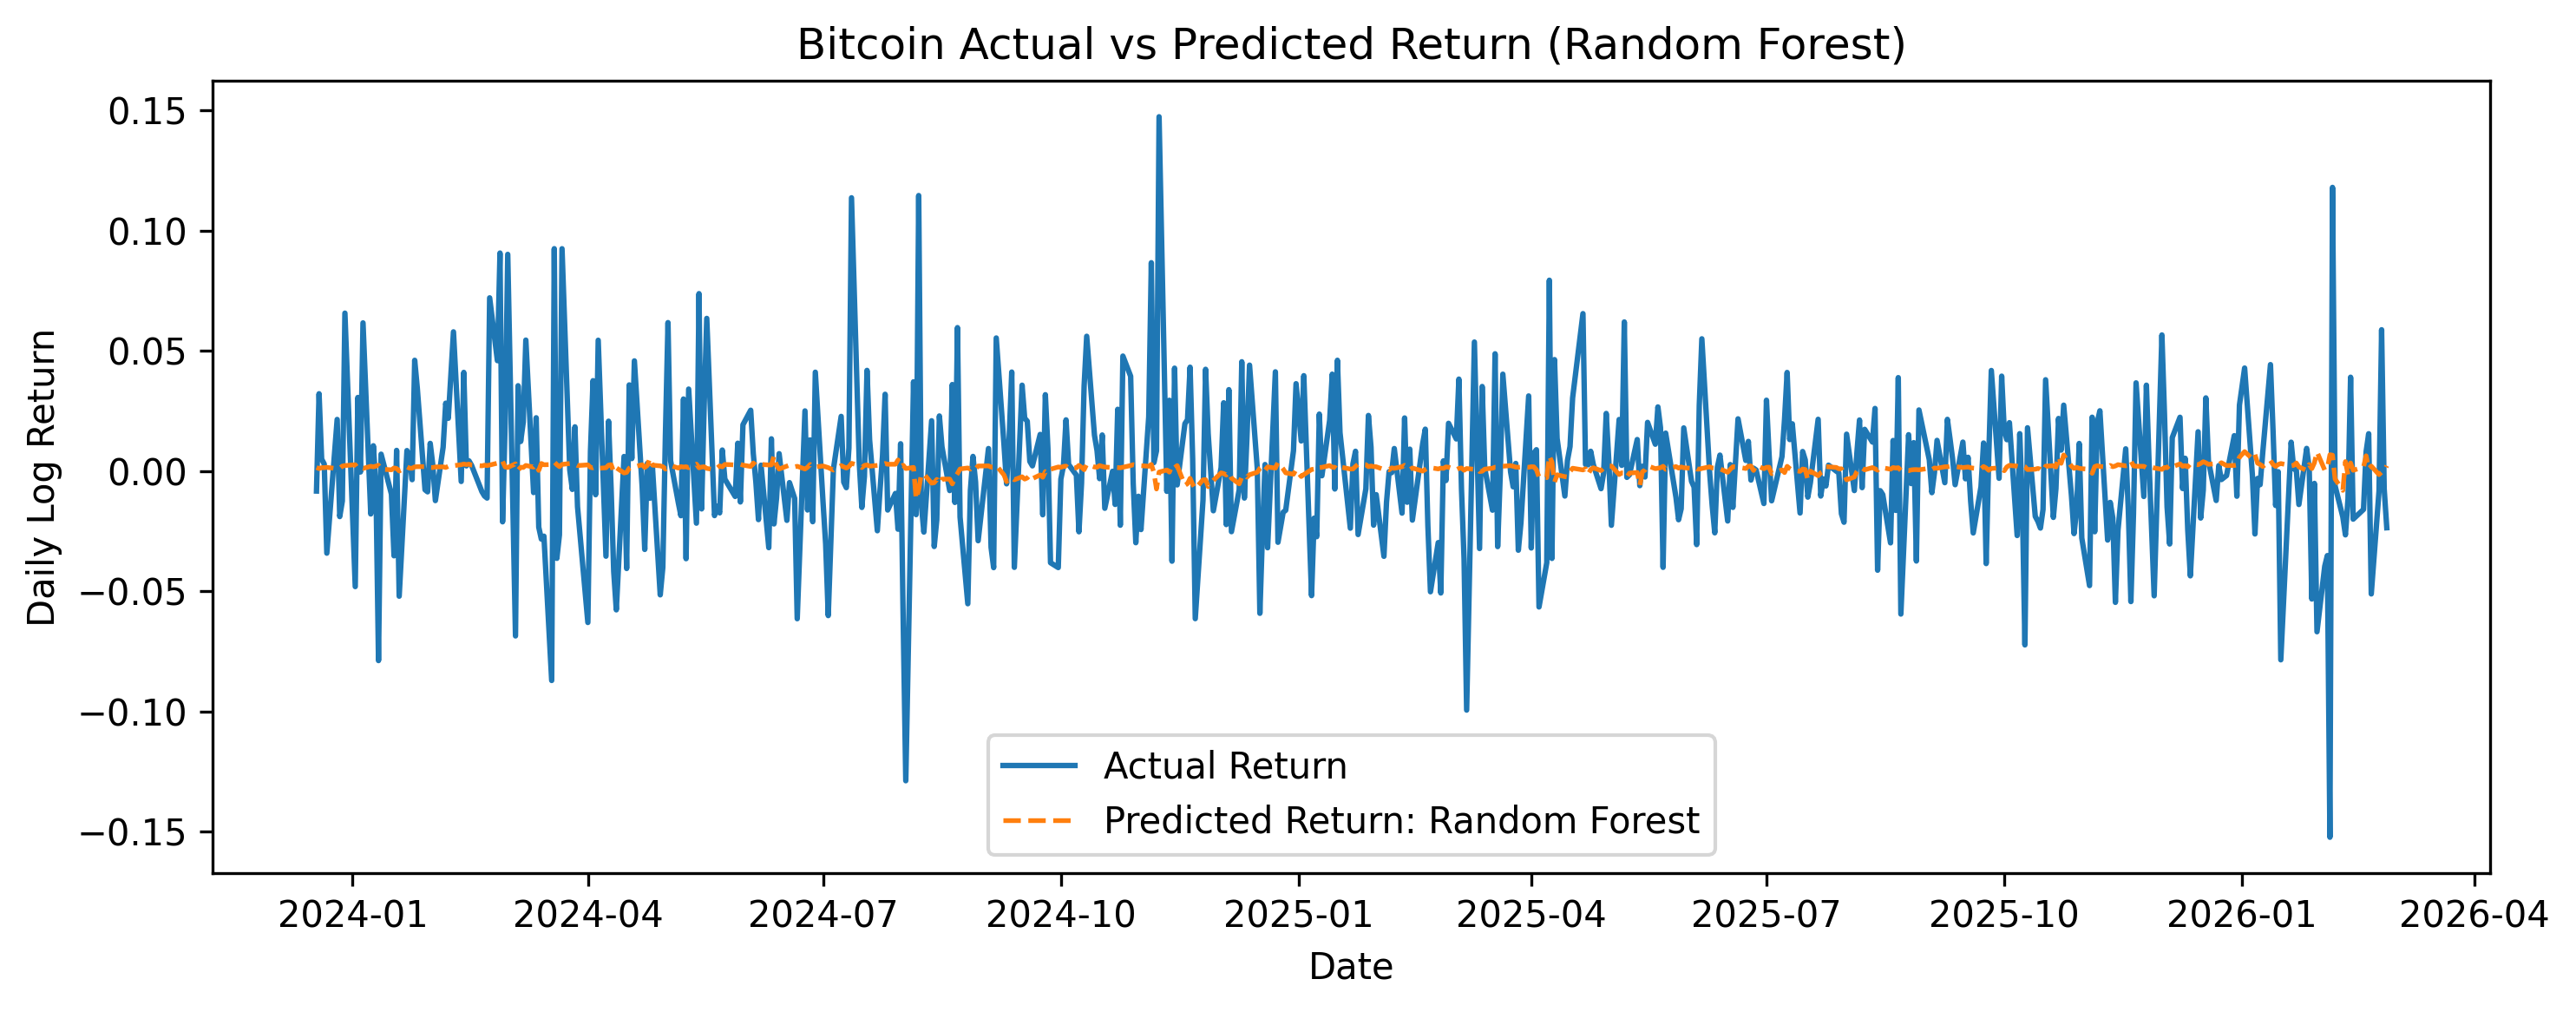
\includegraphics[width=\textwidth, trim=0 6 0 6, clip]{modeling_return_plot/Bitcoin_Random_Forest_return_prediction.png}
        \caption{Bitcoin -- RF}
    \end{subfigure}
    \hspace{0.025\textwidth}
    \begin{subfigure}[t]{0.29\textwidth}
        \centering
        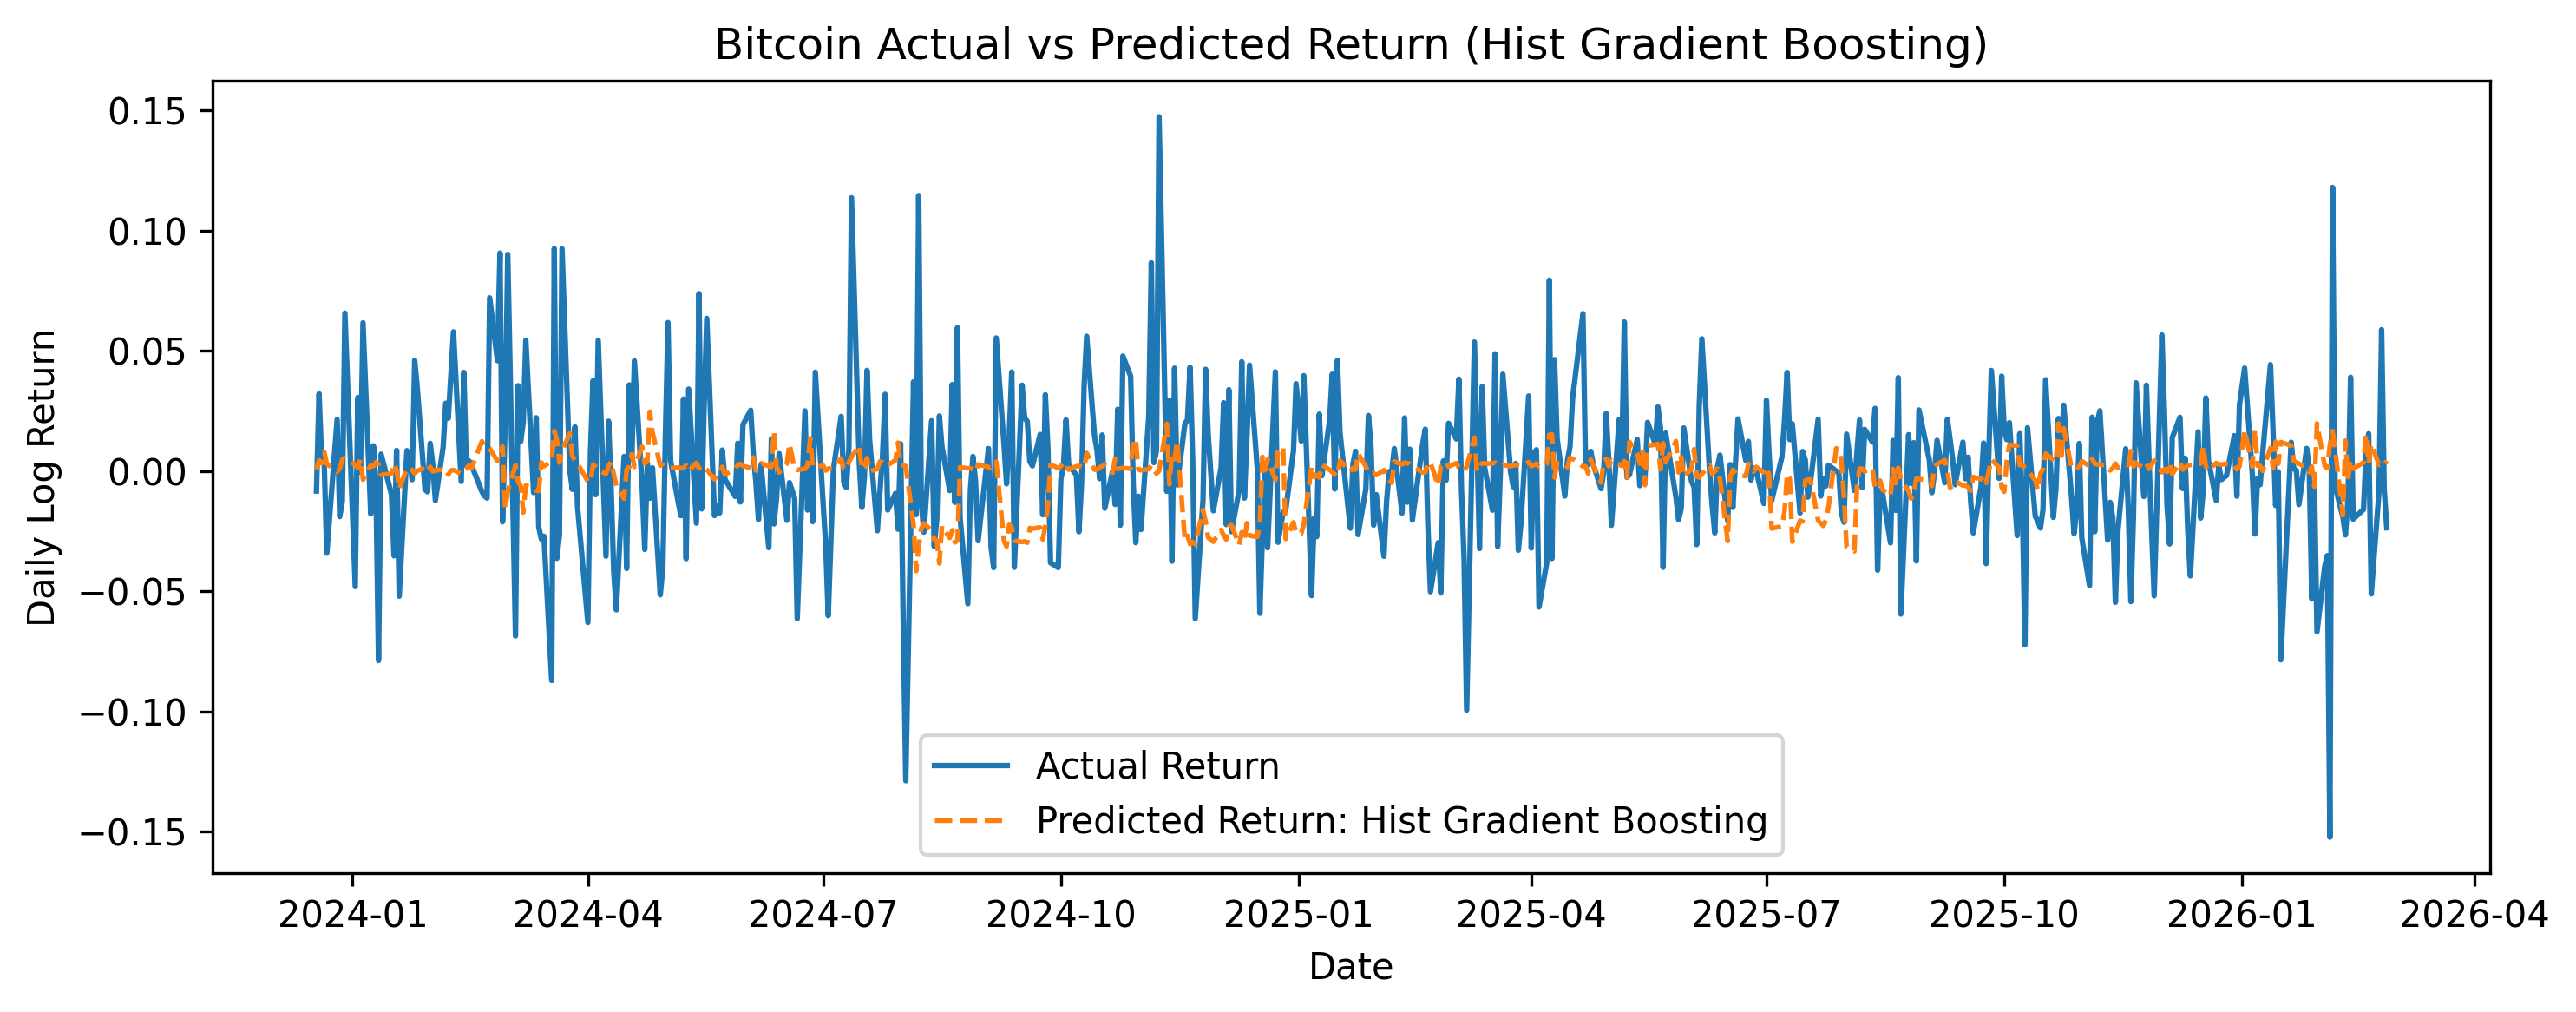
\includegraphics[width=\textwidth, trim=0 6 0 6, clip]{modeling_return_plot/Bitcoin_Hist_Gradient_Boosting_return_prediction.png}
        \caption{Bitcoin -- HGB}
    \end{subfigure}

    \vspace{0.20cm}

    % ---------------- Ethereum ----------------
    \begin{subfigure}[t]{0.29\textwidth}
        \centering
        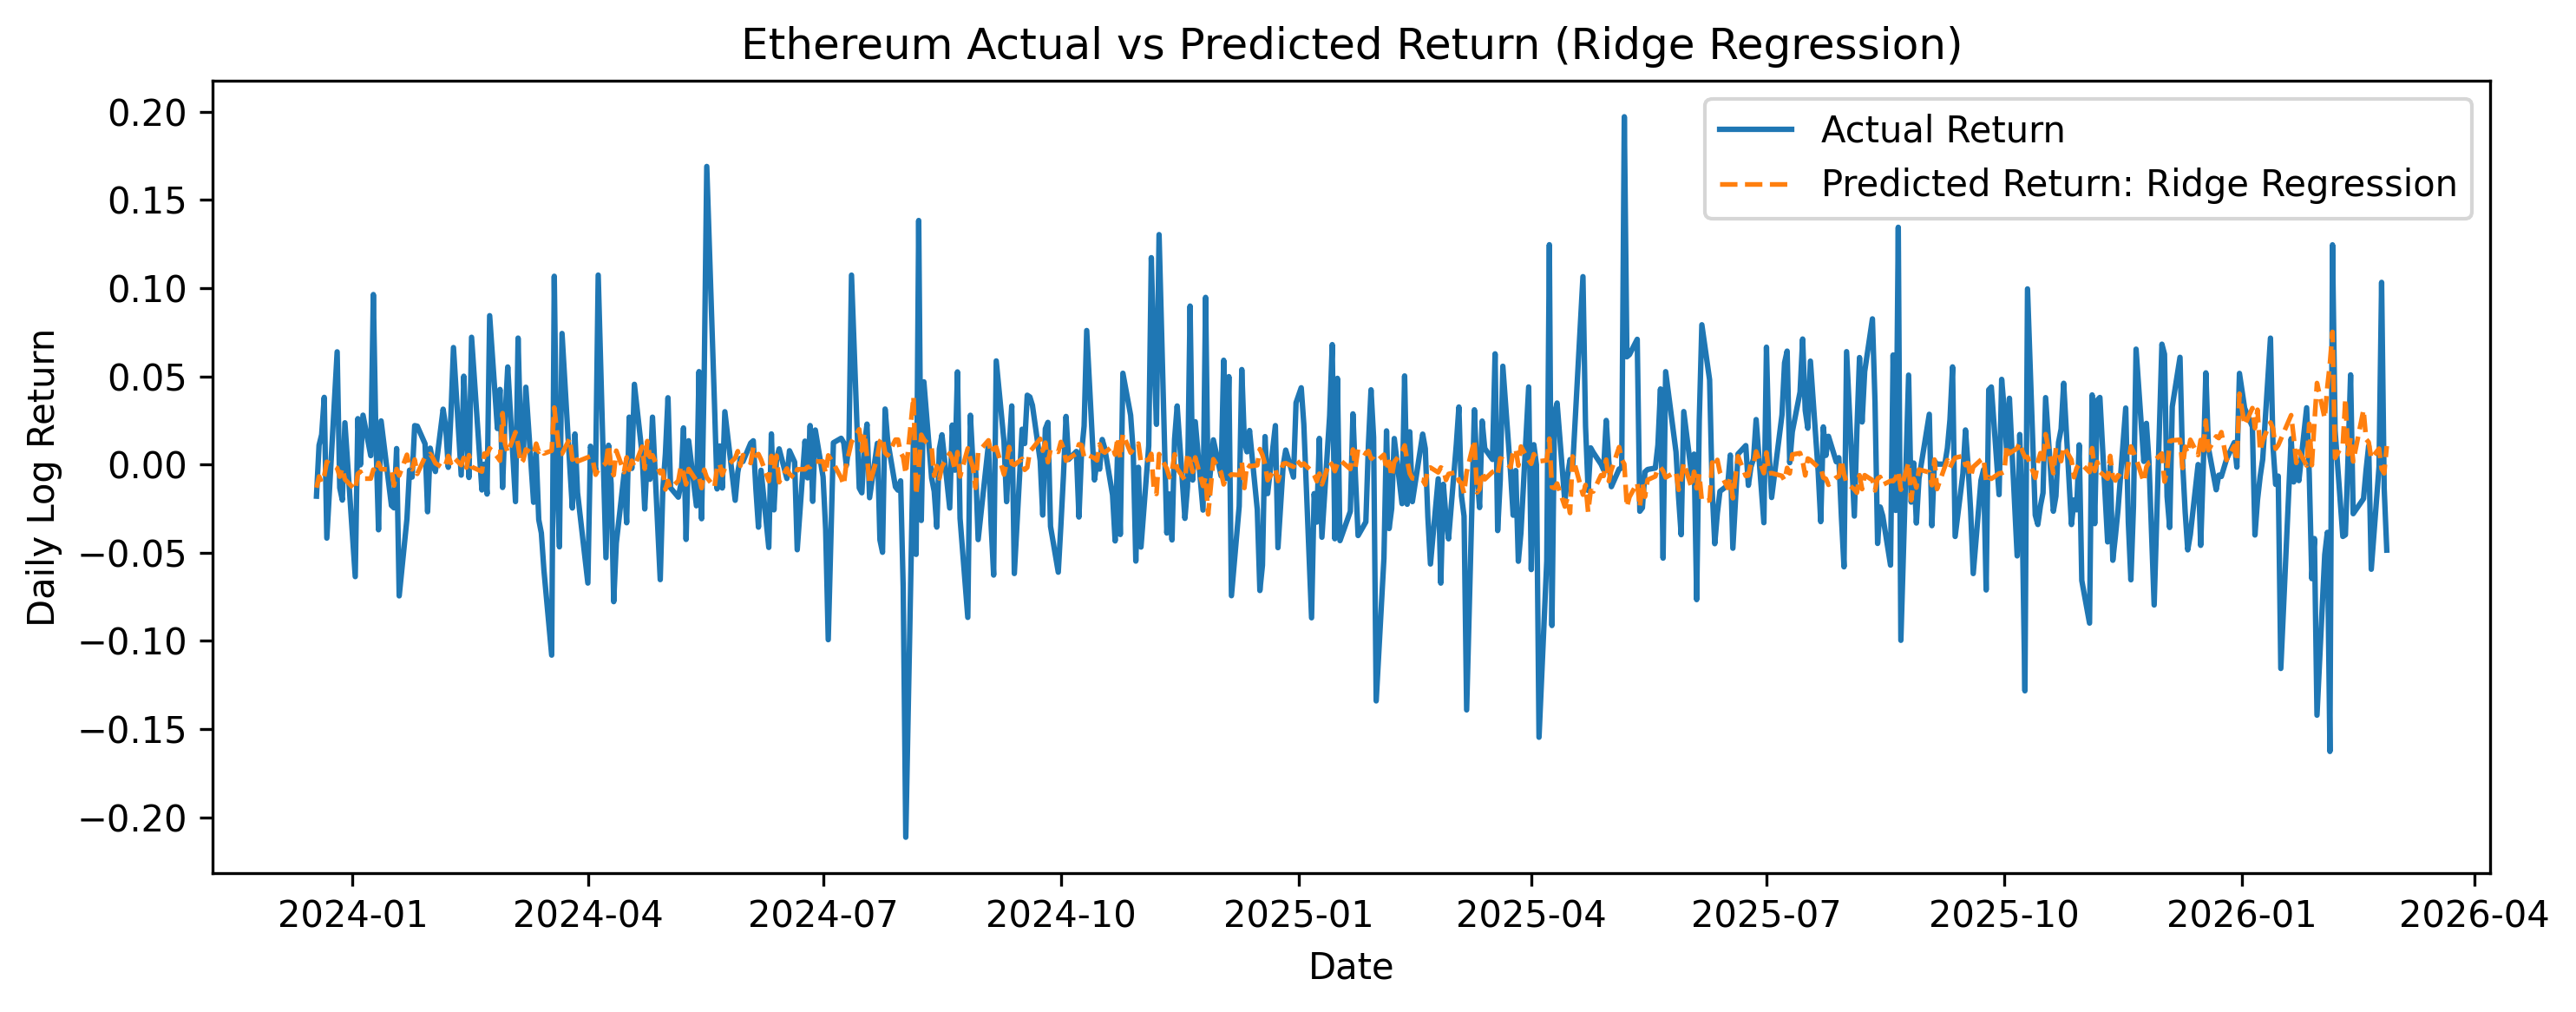
\includegraphics[width=\textwidth, trim=0 6 0 6, clip]{modeling_return_plot/Ethereum_Ridge_Regression_return_prediction.png}
        \caption{Ethereum -- Ridge}
    \end{subfigure}
    \hspace{0.025\textwidth}
    \begin{subfigure}[t]{0.29\textwidth}
        \centering
        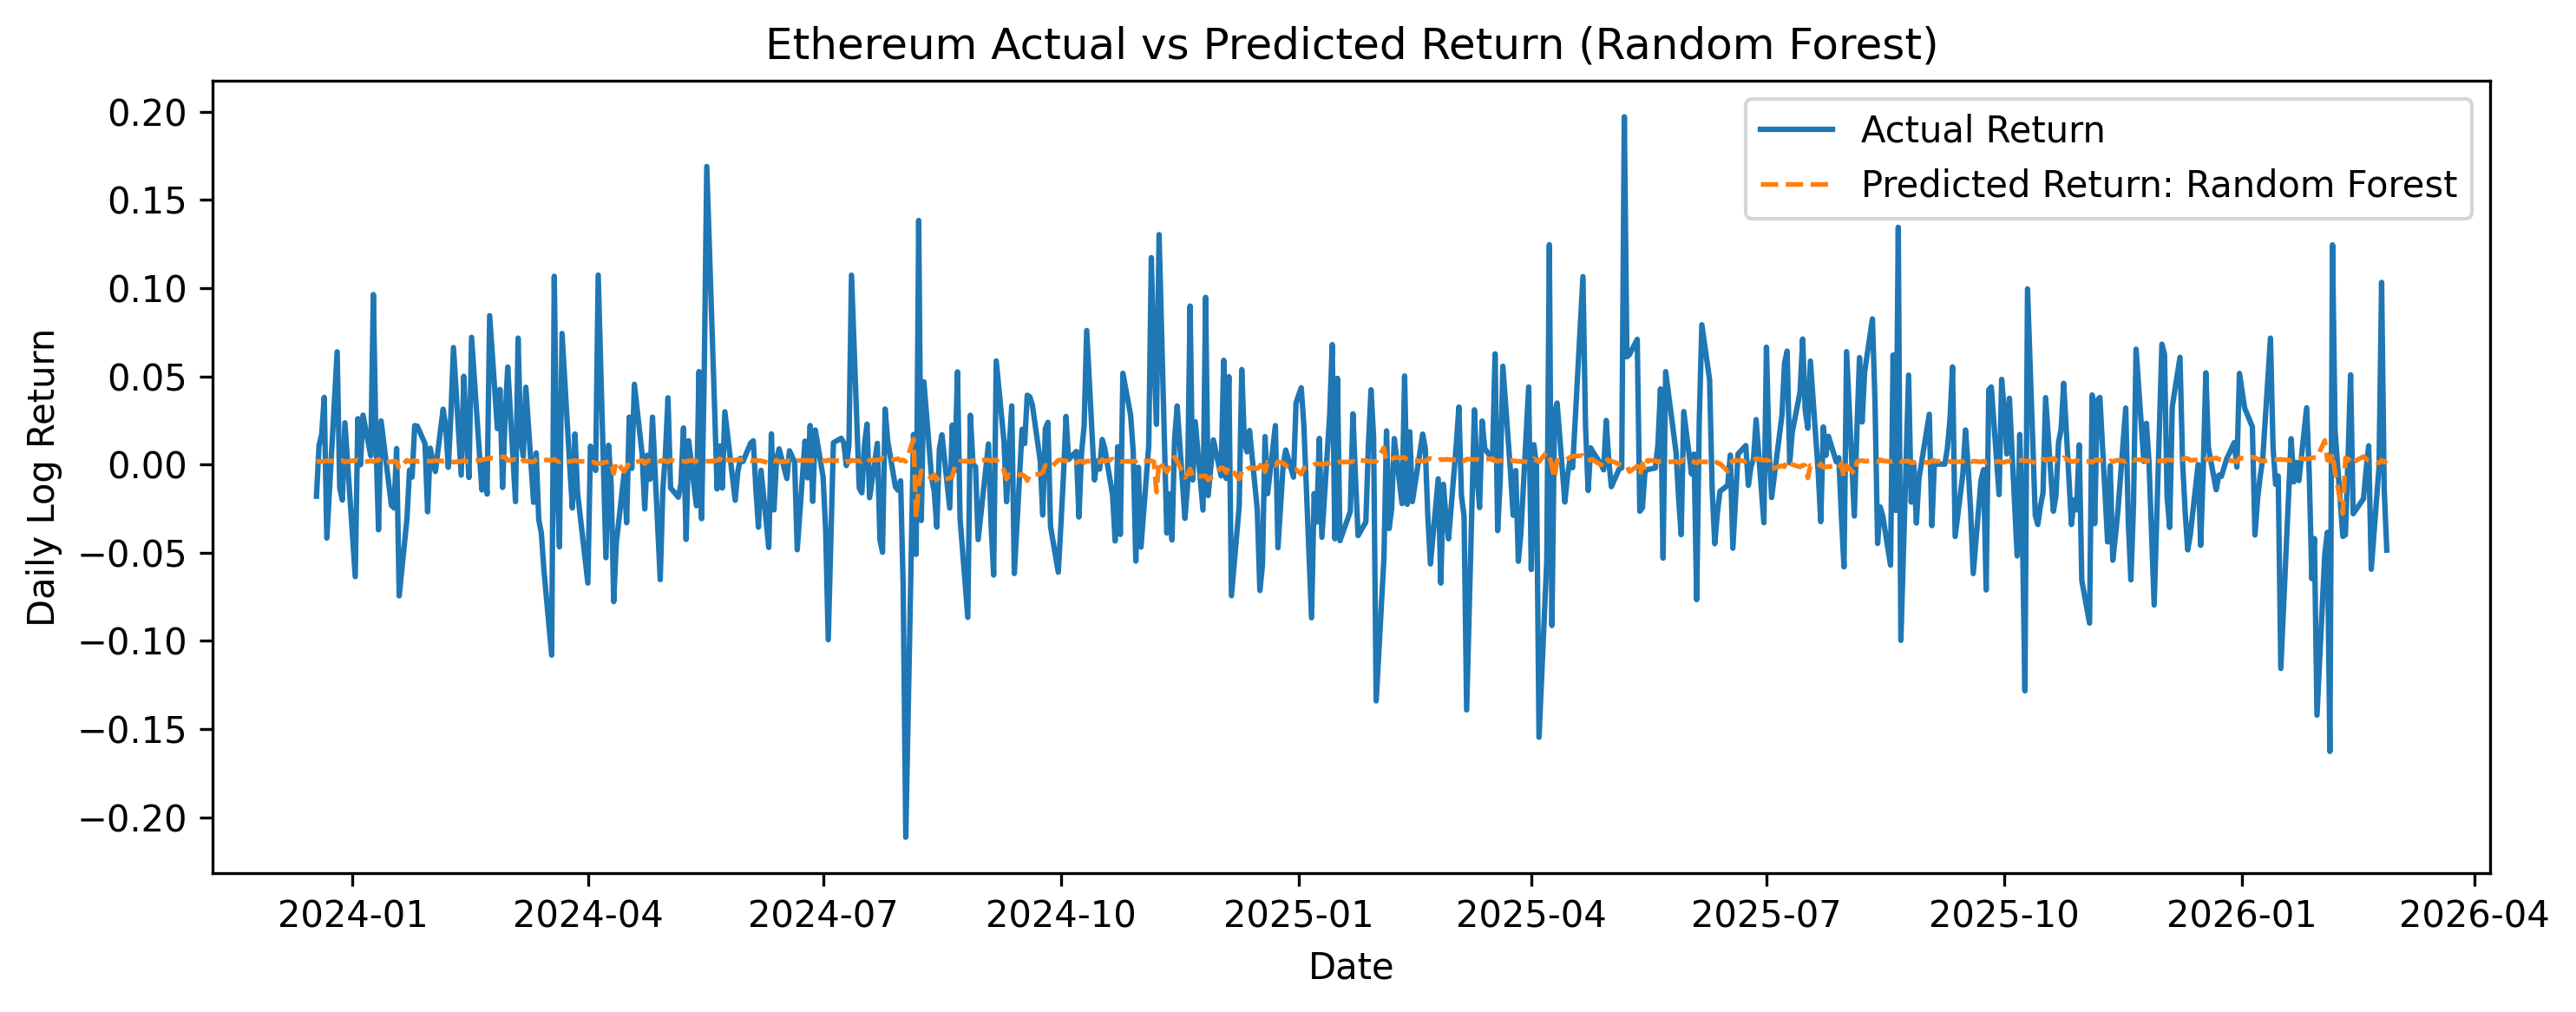
\includegraphics[width=\textwidth, trim=0 6 0 6, clip]{modeling_return_plot/Ethereum_Random_Forest_return_prediction.png}
        \caption{Ethereum -- RF}
    \end{subfigure}
    \hspace{0.025\textwidth}
    \begin{subfigure}[t]{0.29\textwidth}
        \centering
        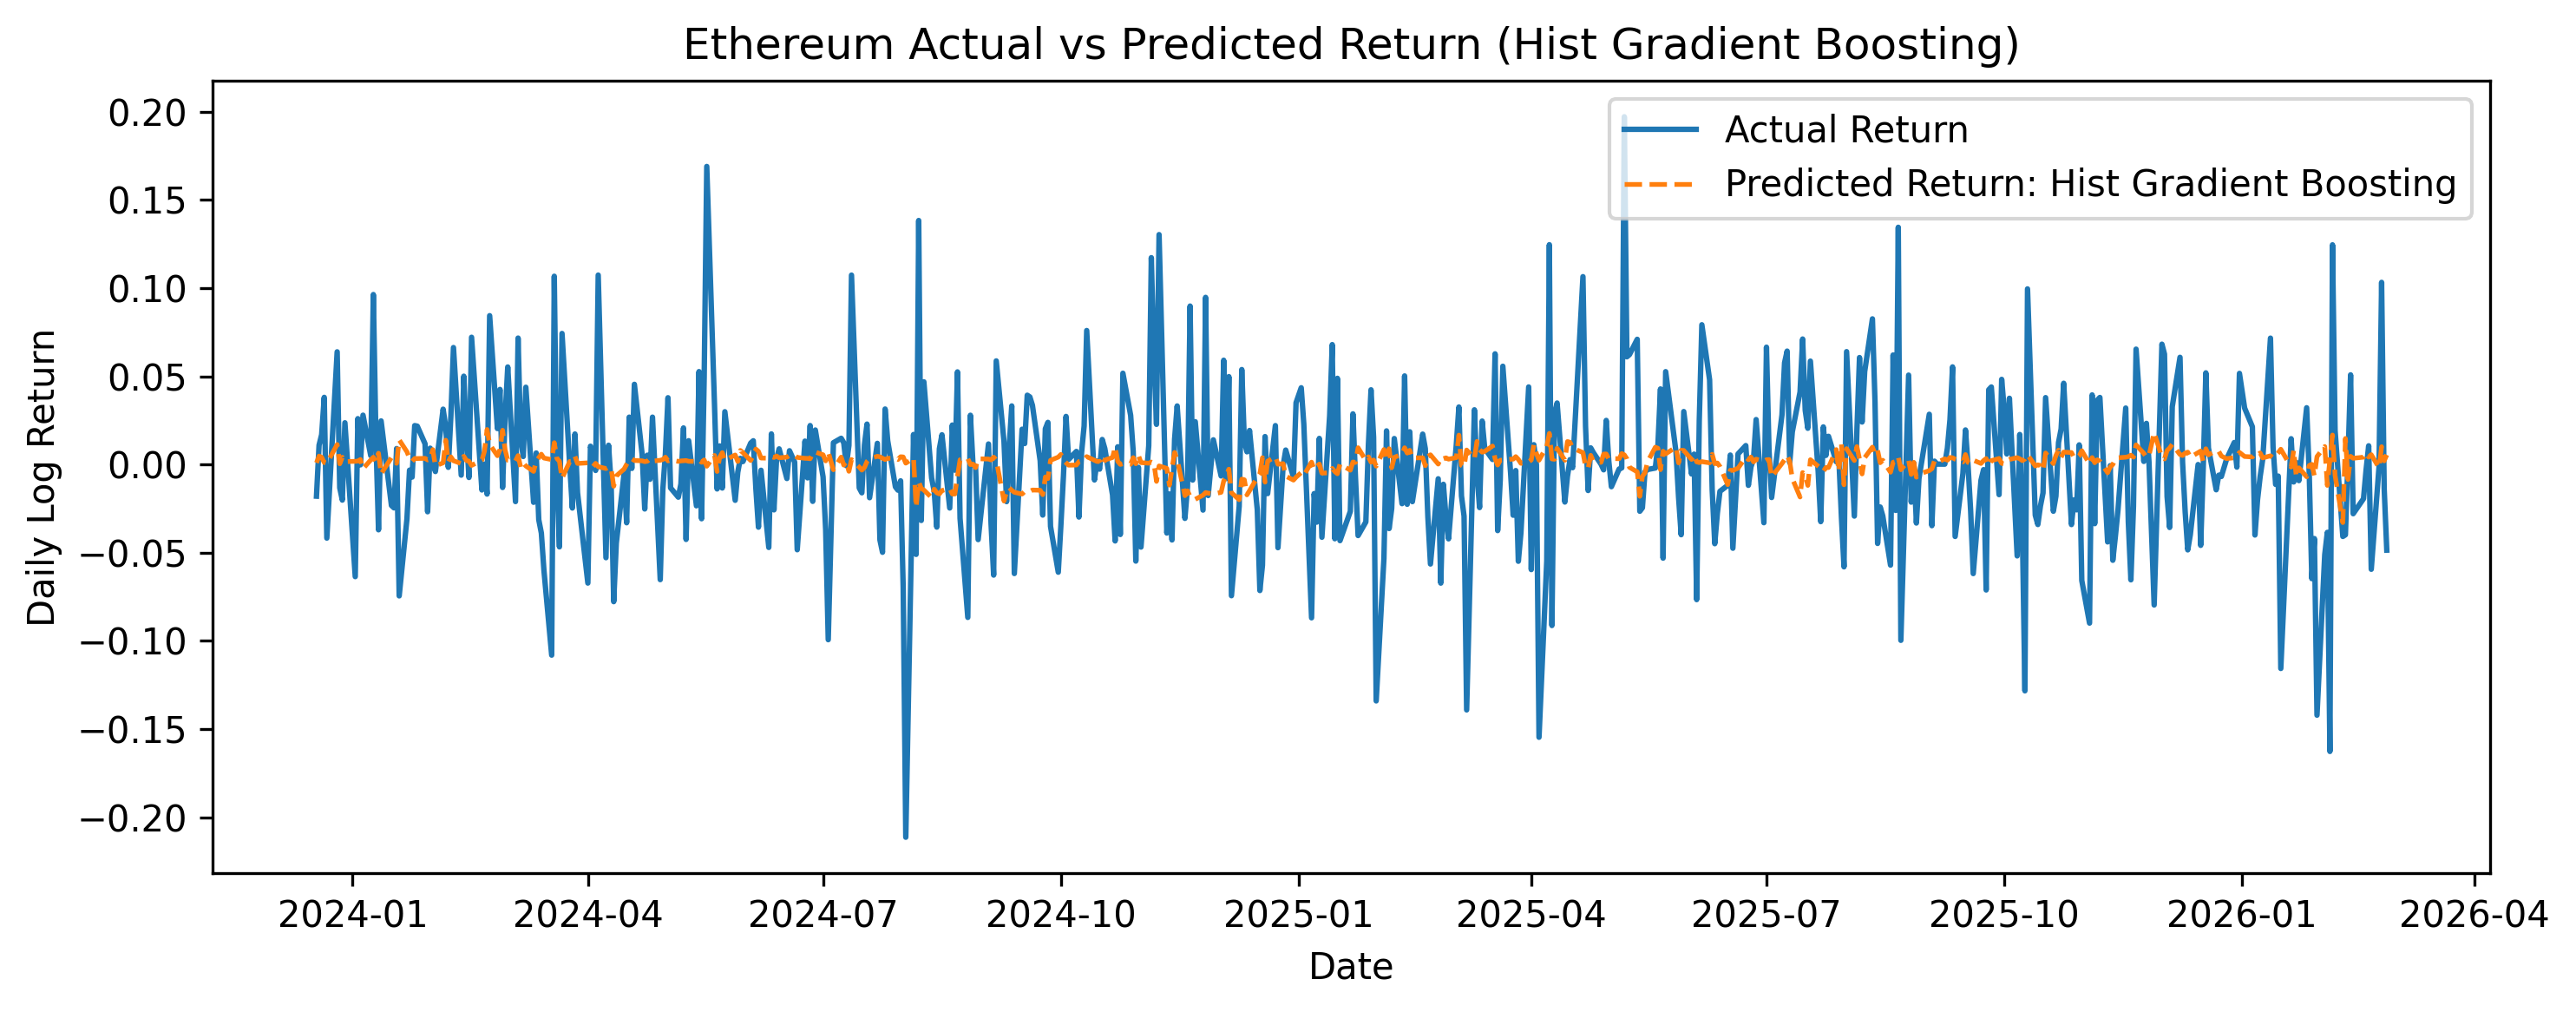
\includegraphics[width=\textwidth, trim=0 6 0 6, clip]{modeling_return_plot/Ethereum_Hist_Gradient_Boosting_return_prediction.png}
        \caption{Ethereum -- HGB}
    \end{subfigure}

    \vspace{0.12cm}
    \caption{Actual vs Predicted Returns for Cryptocurrencies}
    \label{fig:return_predictions_crypto}
\end{figure}

Figure~\ref{fig:return_predictions_crypto} reports the return prediction plots for Bitcoin and Ethereum. These two assets have the largest return fluctuations among the six assets, so their return prediction task is more difficult. The plots help show that even when the price prediction paths appear close, the actual return-level prediction remains challenging because daily cryptocurrency returns contain stronger noise and more extreme movements.

Overall, the return prediction plots provide a necessary check before interpreting the price prediction results. If only price plots are shown, the predicted and actual price paths may look very close because price is a cumulative series. By also showing return plots, we can more honestly evaluate the model's direct forecasting target and reduce the risk of overstating model performance.

\subsection{Price Prediction Plots for All Models}

To make the supervised learning results easier to interpret, the predicted next-day log returns were converted back into predicted prices using

\begin{equation}
\hat{P}_{t+1}
=
P_t \exp(\hat{r}_{t+1}).
\end{equation}

The actual and predicted prices were normalized to start at 100. Figures \ref{fig:price_predictions_crypto}, \ref{fig:price_predictions_metals}, and \ref{fig:price_predictions_macro} compare the actual price path with the predicted price path for each asset under all three supervised models. Each row contains the three models for the same asset: Ridge Regression, Random Forest, and Hist Gradient Boosting.

% ------------------------------------------------------------
% Figure: Bitcoin and Ethereum
% ------------------------------------------------------------

\begin{figure}[htbp]
    \centering

    \begin{subfigure}[t]{0.305\textwidth}
        \centering
        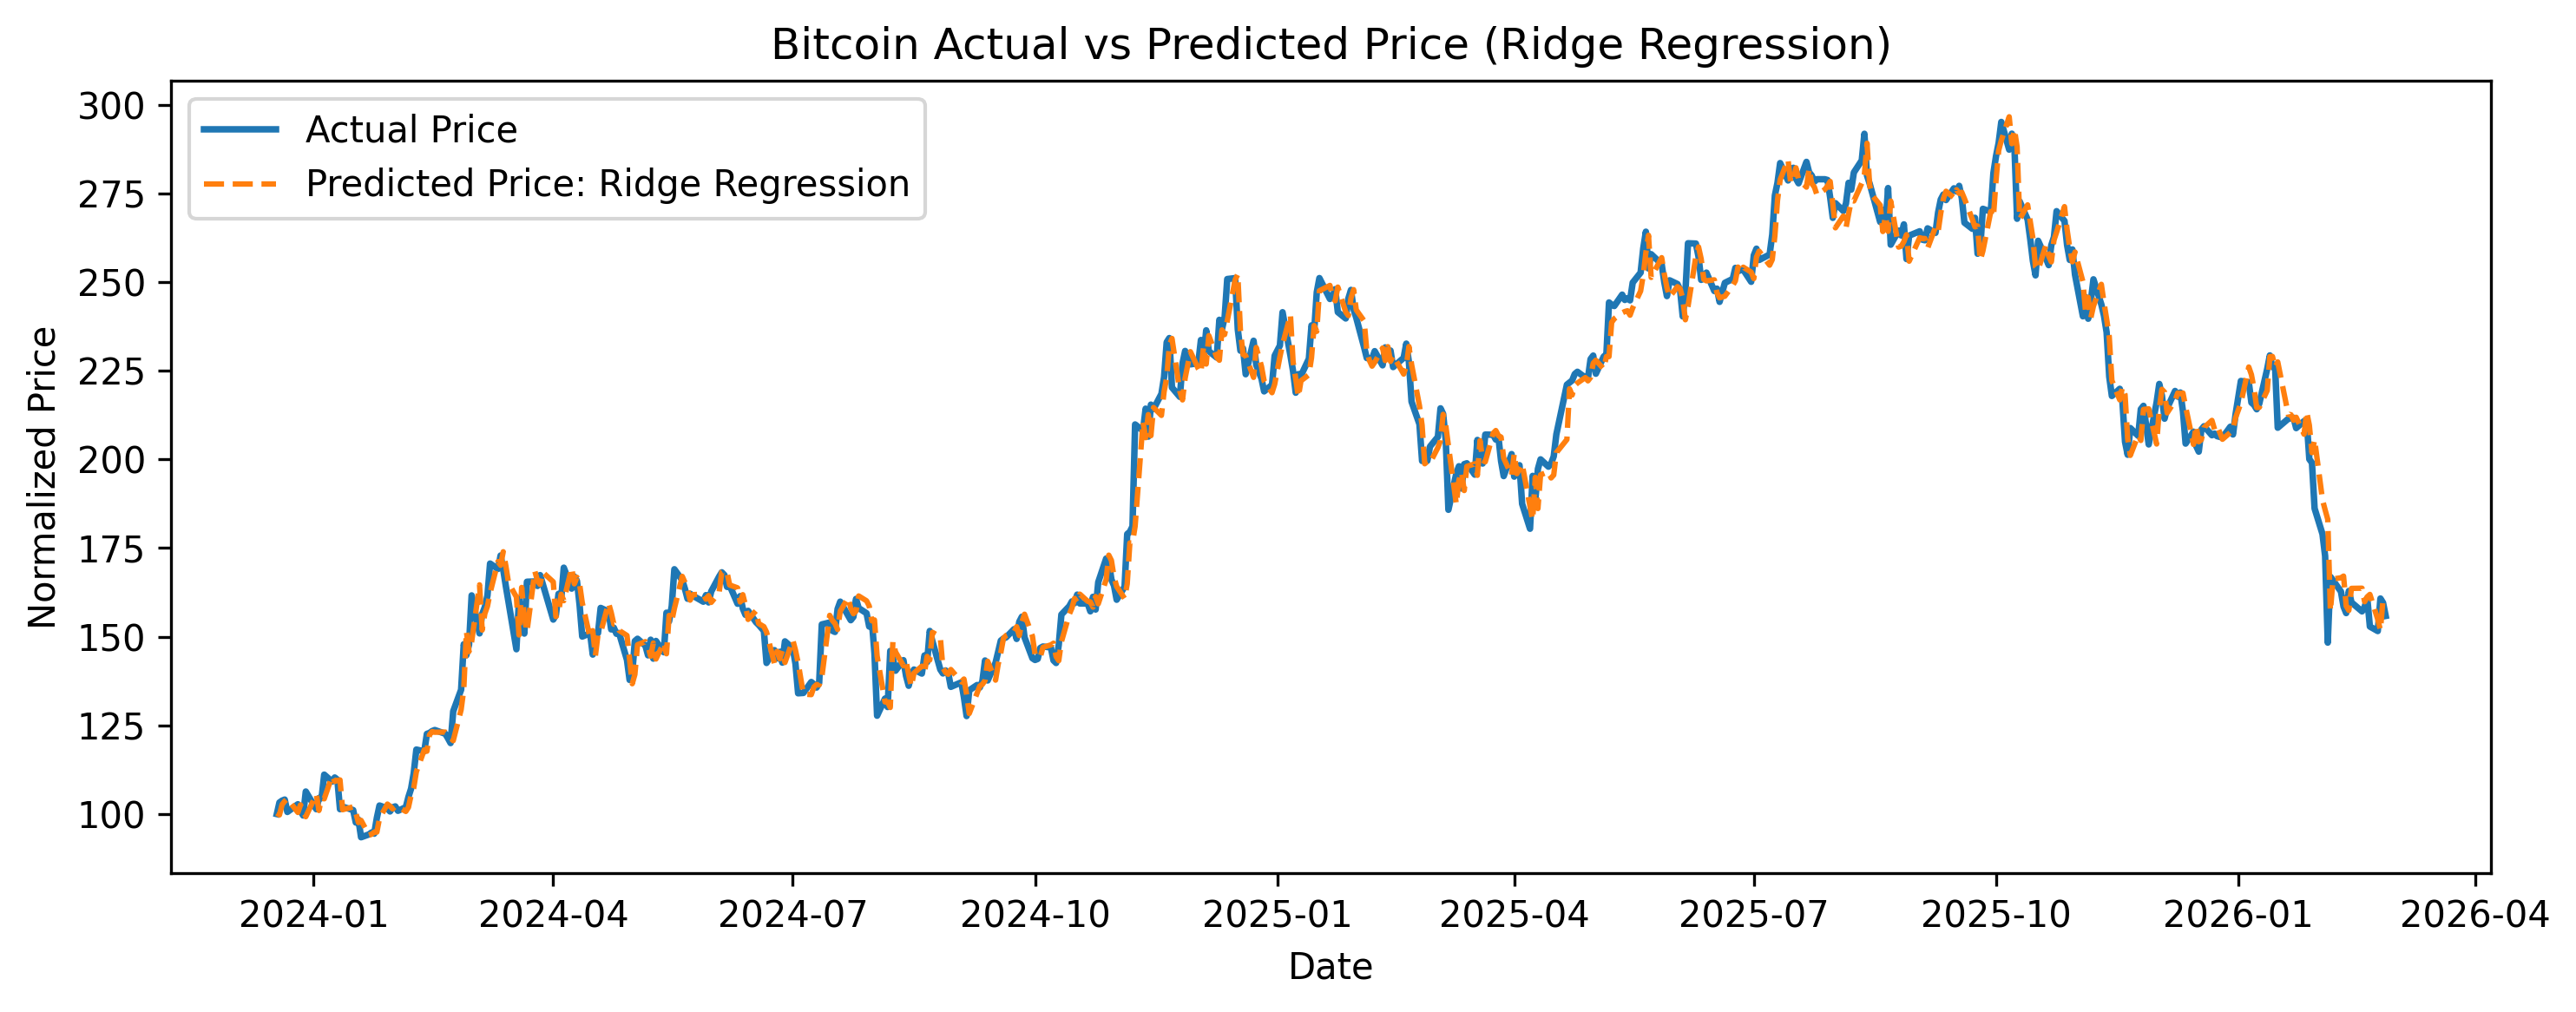
\includegraphics[width=\textwidth]{modeling_plot/Bitcoin_Ridge_Regression_price_prediction.png}
        \caption{Bitcoin -- Ridge}
    \end{subfigure}
    \hfill
    \begin{subfigure}[t]{0.305\textwidth}
        \centering
        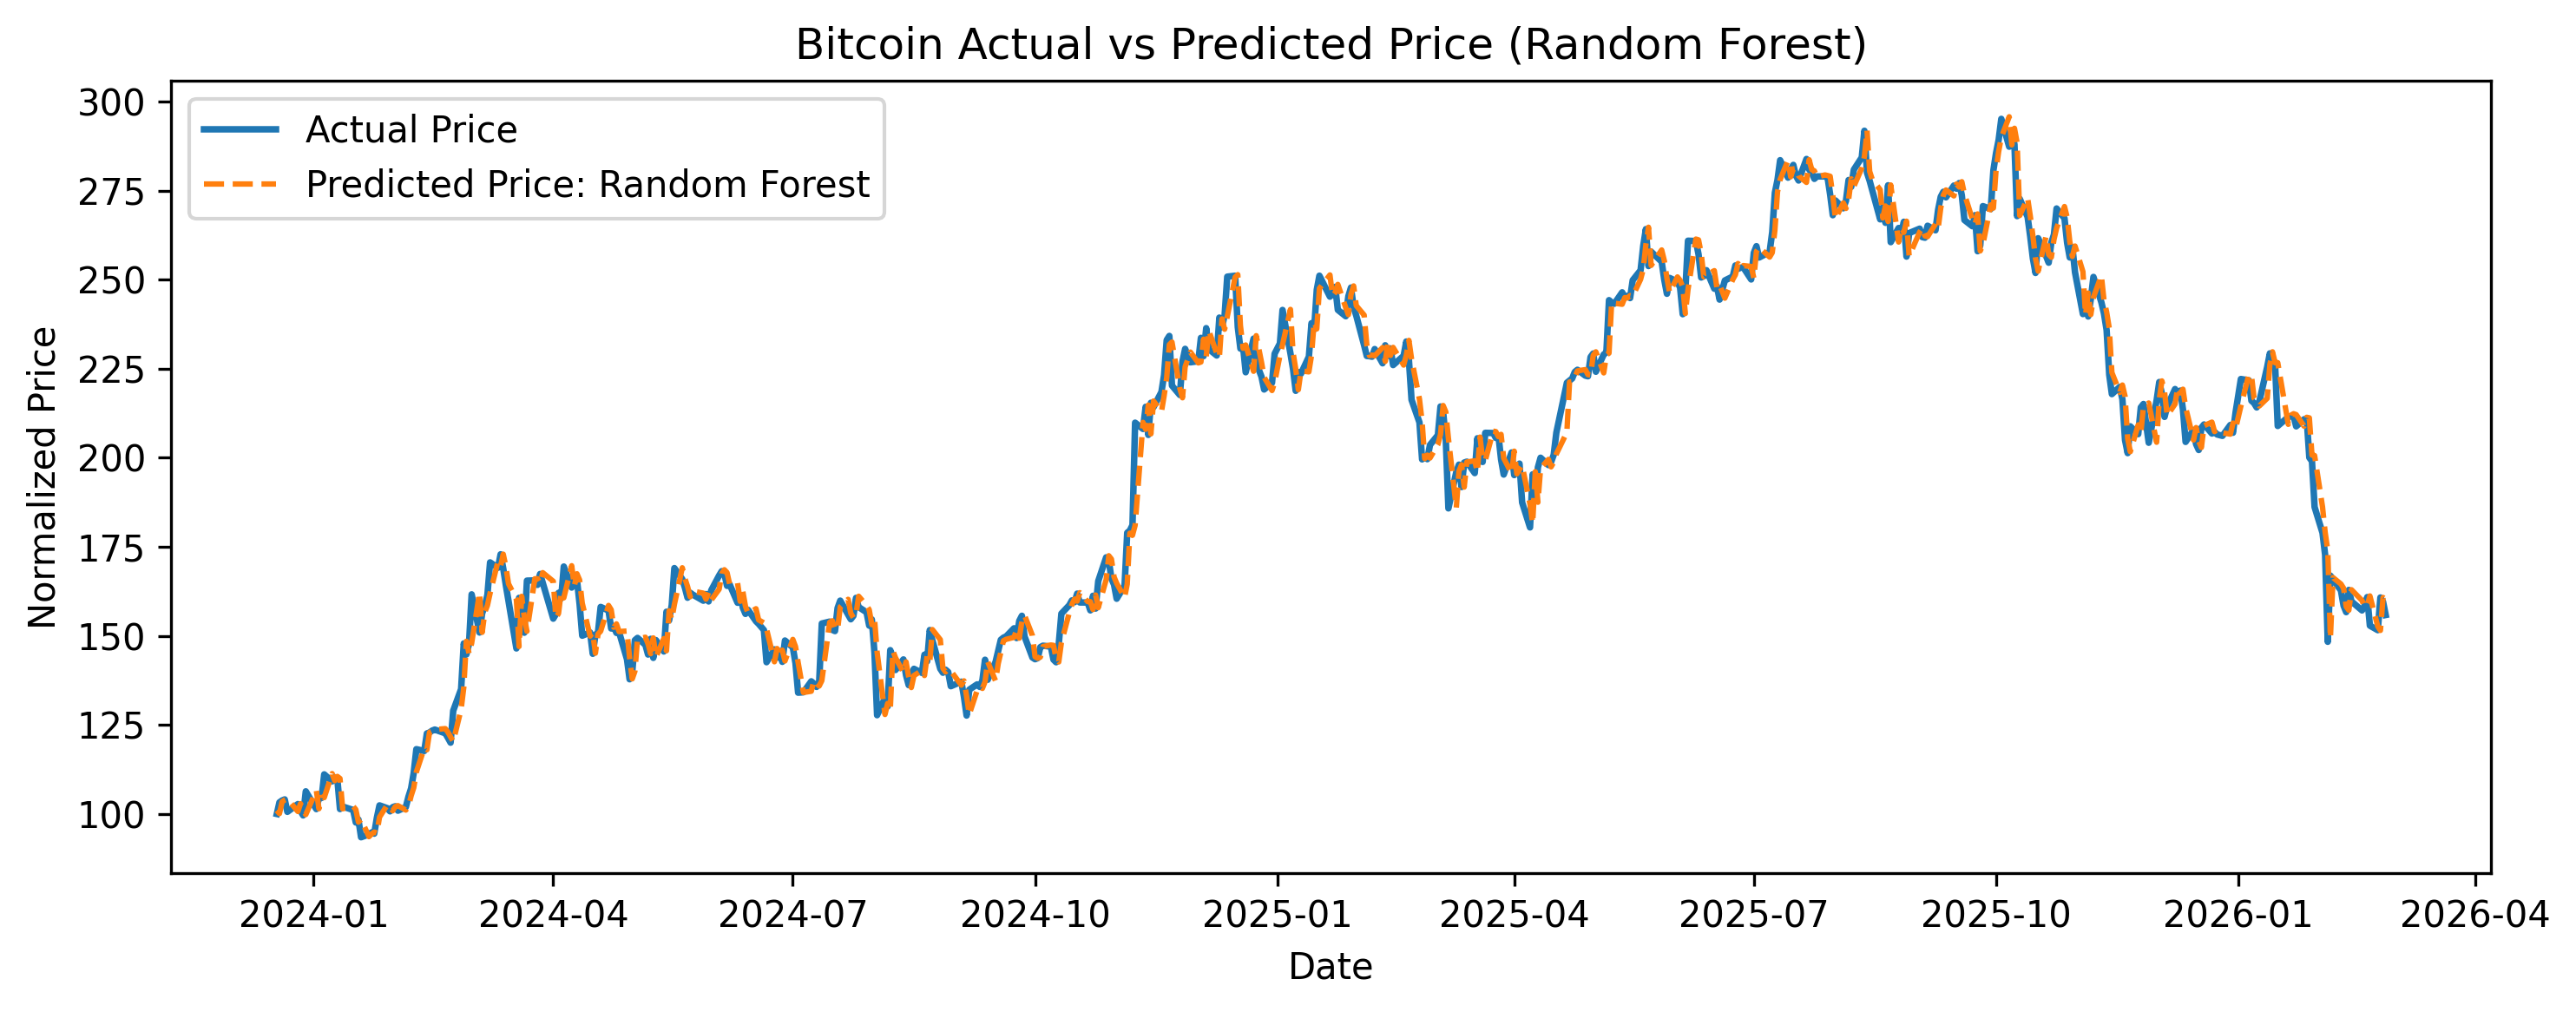
\includegraphics[width=\textwidth]{modeling_plot/Bitcoin_Random_Forest_price_prediction.png}
        \caption{Bitcoin -- RF}
    \end{subfigure}
    \hfill
    \begin{subfigure}[t]{0.305\textwidth}
        \centering
        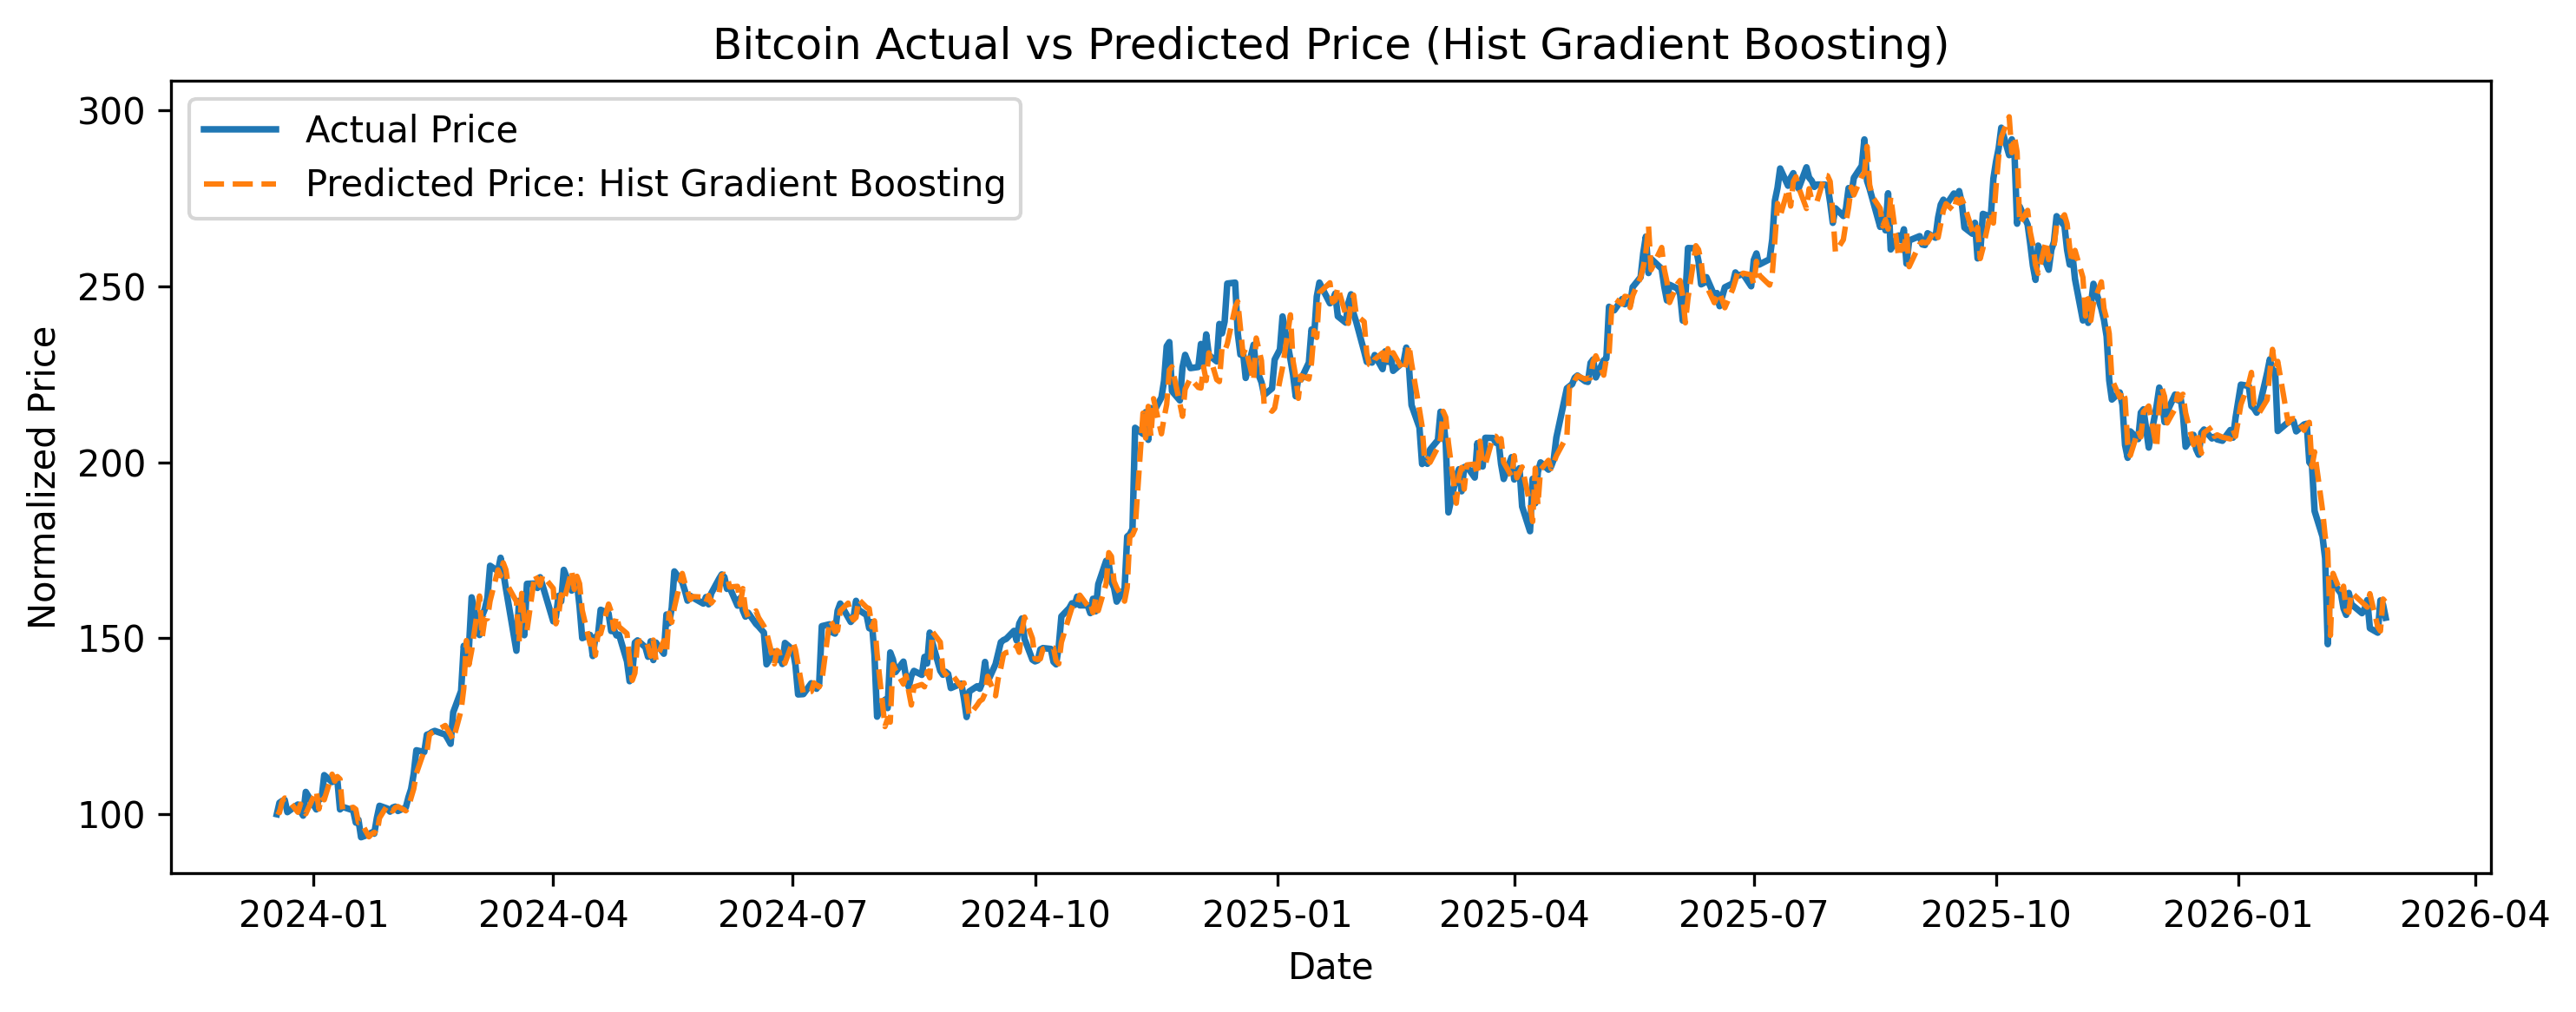
\includegraphics[width=\textwidth]{modeling_plot/Bitcoin_Hist_Gradient_Boosting_price_prediction.png}
        \caption{Bitcoin -- HGB}
    \end{subfigure}

    \vspace{0.12cm}

    \begin{subfigure}[t]{0.305\textwidth}
        \centering
        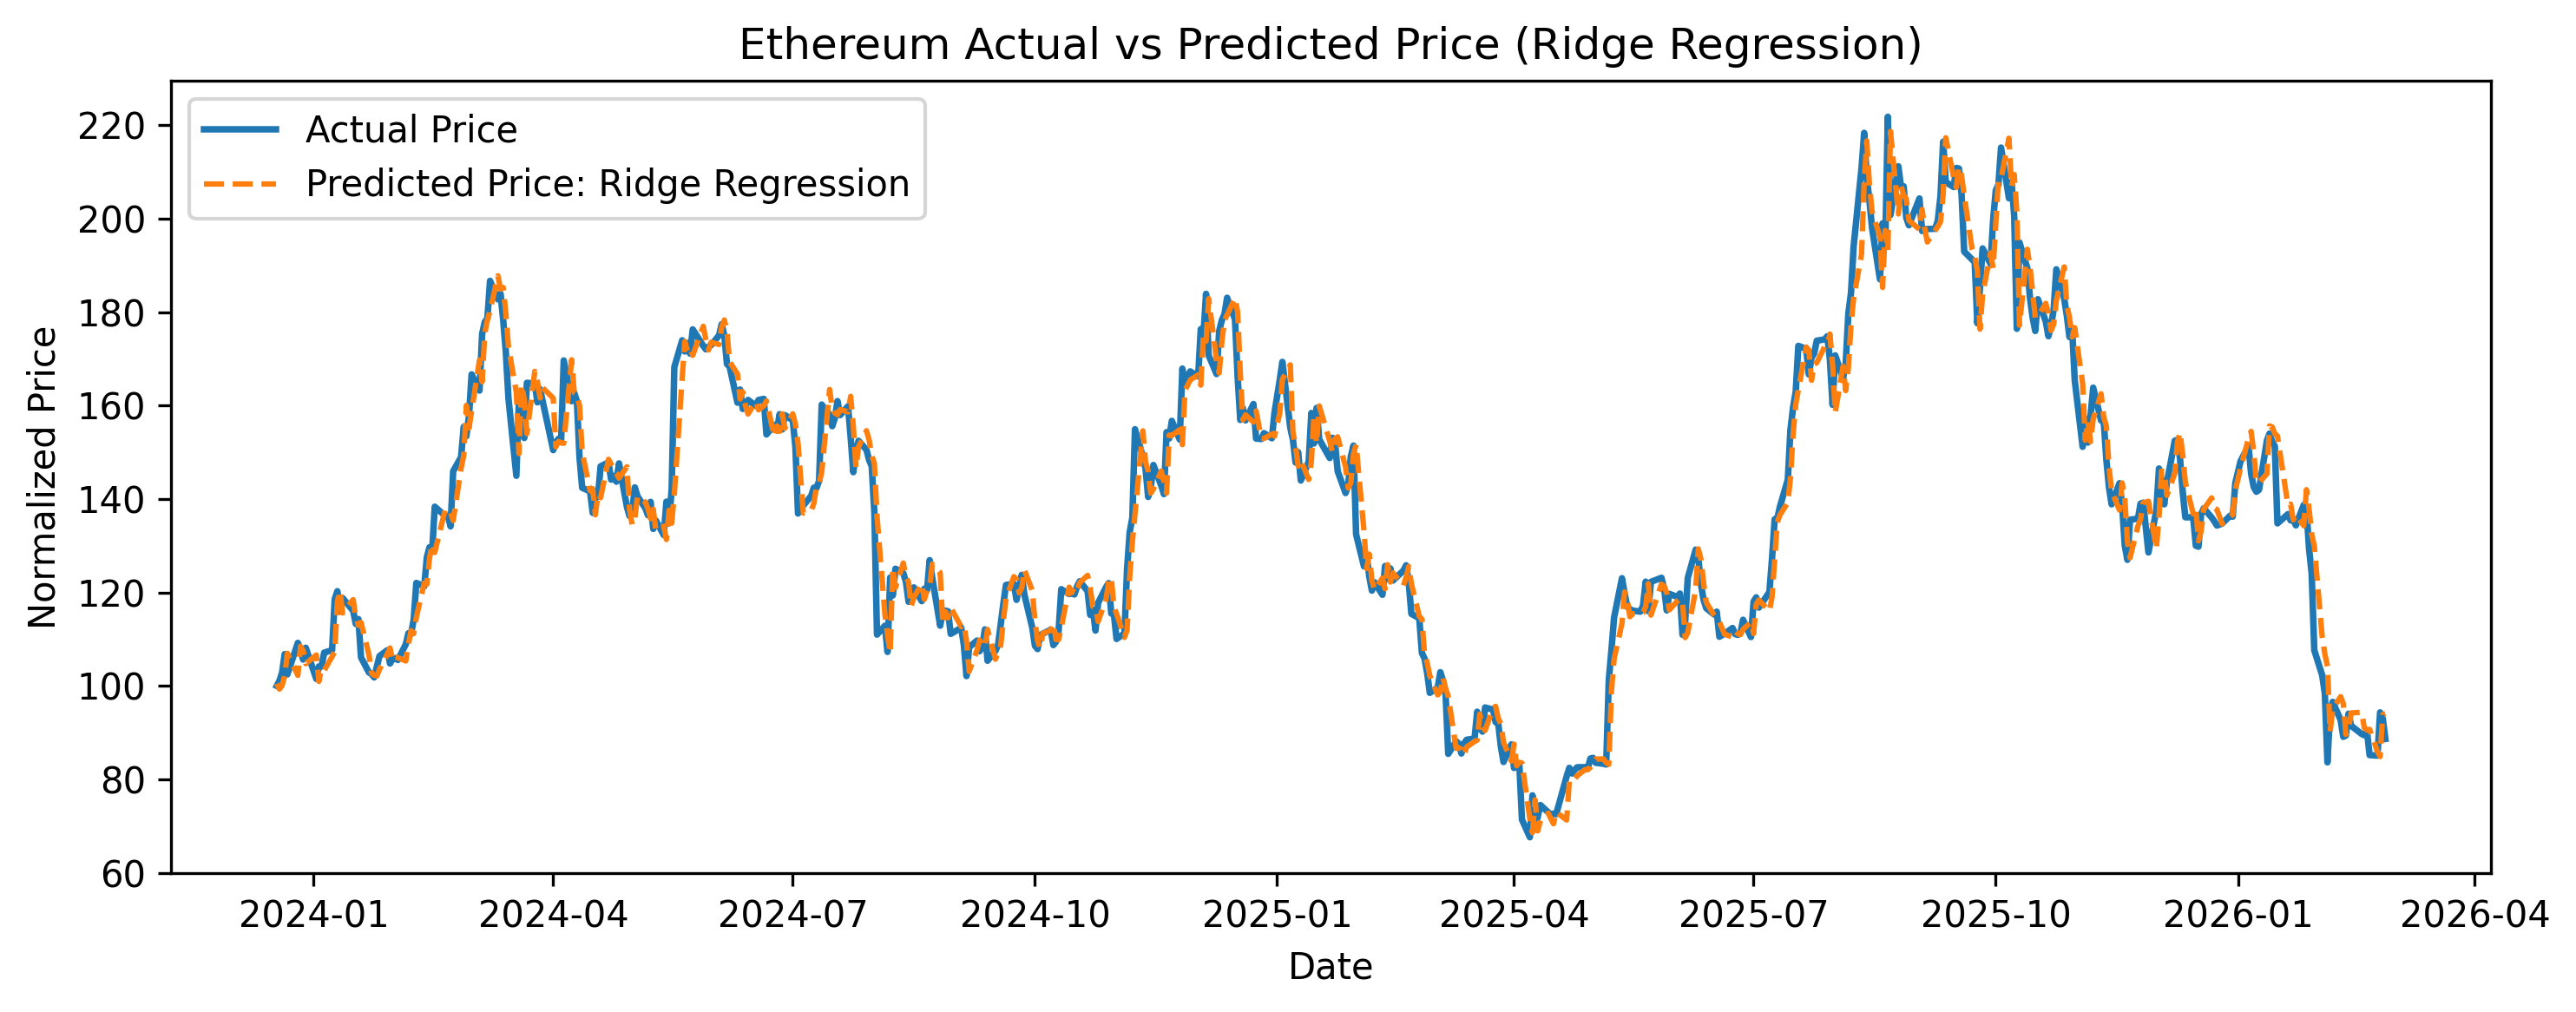
\includegraphics[width=\textwidth]{modeling_plot/Ethereum_Ridge_Regression_price_prediction.png}
        \caption{Ethereum -- Ridge}
    \end{subfigure}
    \hfill
    \begin{subfigure}[t]{0.305\textwidth}
        \centering
        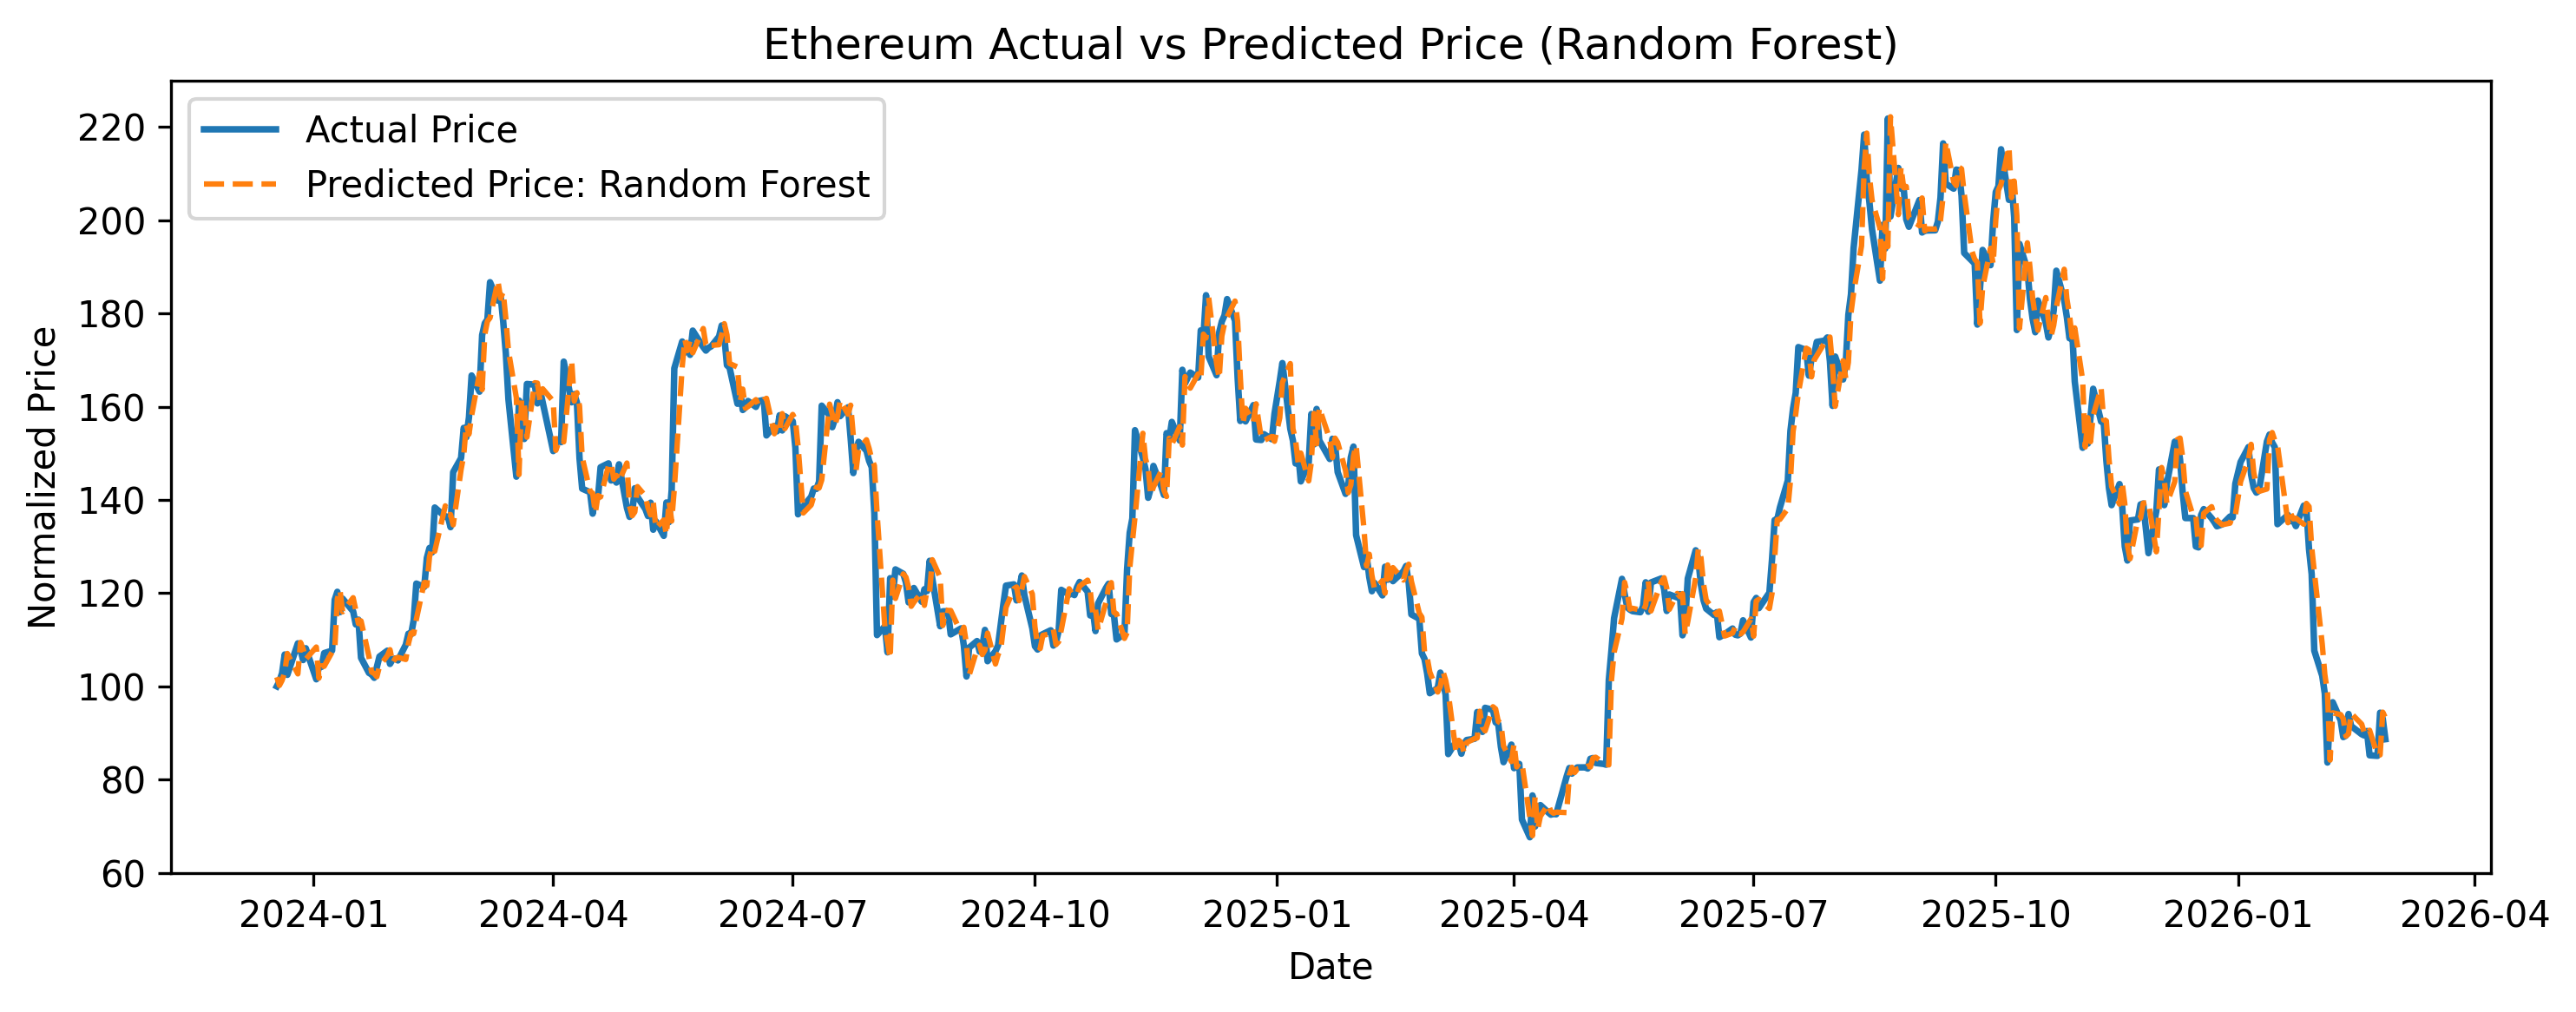
\includegraphics[width=\textwidth]{modeling_plot/Ethereum_Random_Forest_price_prediction.png}
        \caption{Ethereum -- RF}
    \end{subfigure}
    \hfill
    \begin{subfigure}[t]{0.305\textwidth}
        \centering
        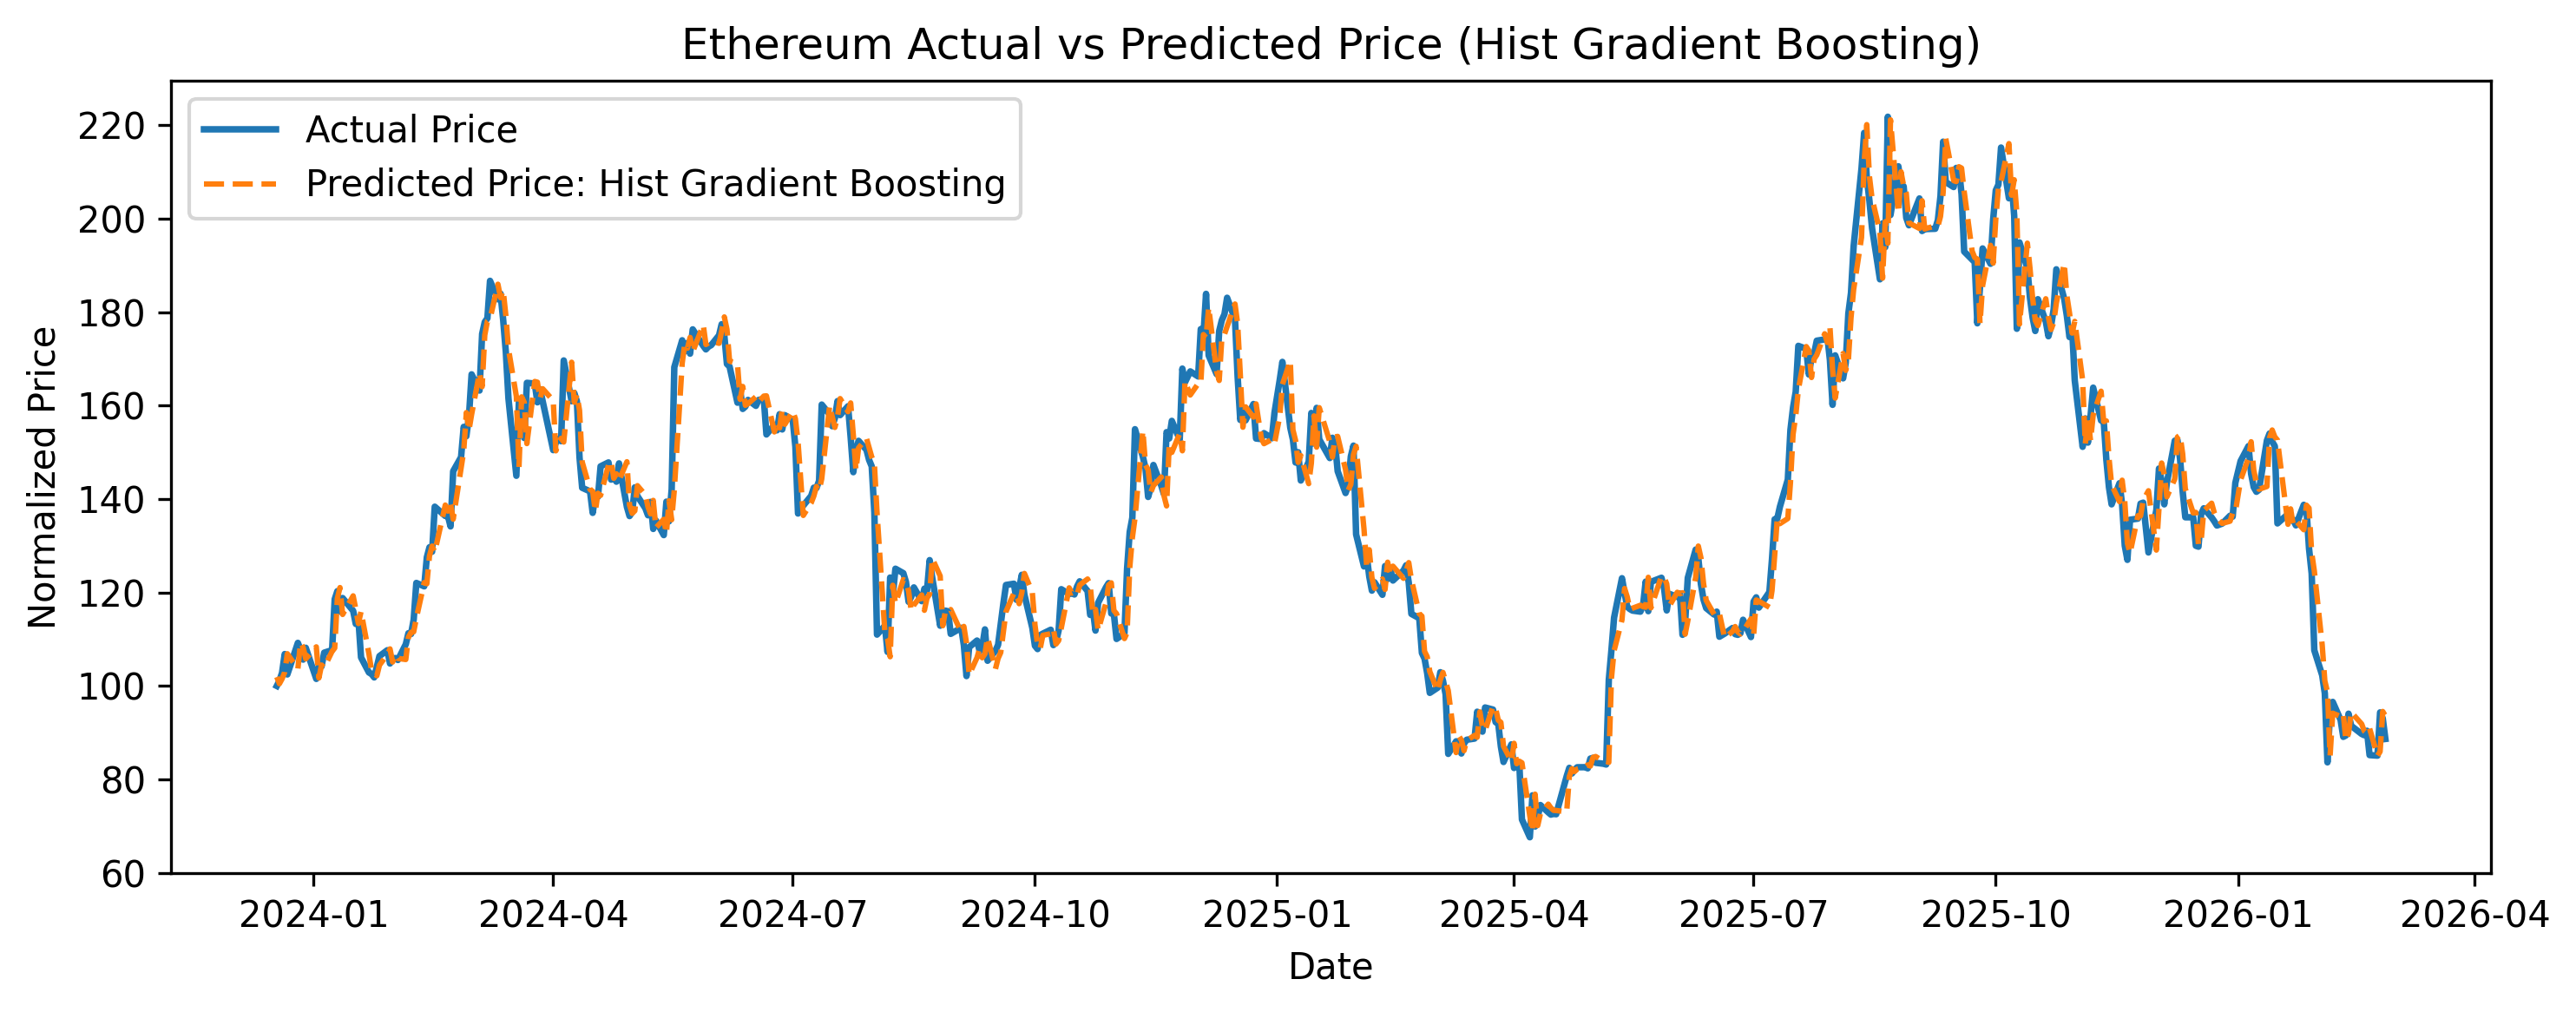
\includegraphics[width=\textwidth]{modeling_plot/Ethereum_Hist_Gradient_Boosting_price_prediction.png}
        \caption{Ethereum -- HGB}
    \end{subfigure}

    \caption{Actual vs Predicted Prices for Cryptocurrencies}
    \label{fig:price_predictions_crypto}
\end{figure}

% ------------------------------------------------------------ 
% Figure: Gold and Silver
% ------------------------------------------------------------

\begin{figure}[H]
    \centering
    \captionsetup[subfigure]{skip=4pt}
    \setlength{\abovecaptionskip}{5pt}
    \setlength{\belowcaptionskip}{3pt}

    % ---------------- Gold ----------------
    \begin{subfigure}[t]{0.29\textwidth}
        \centering
        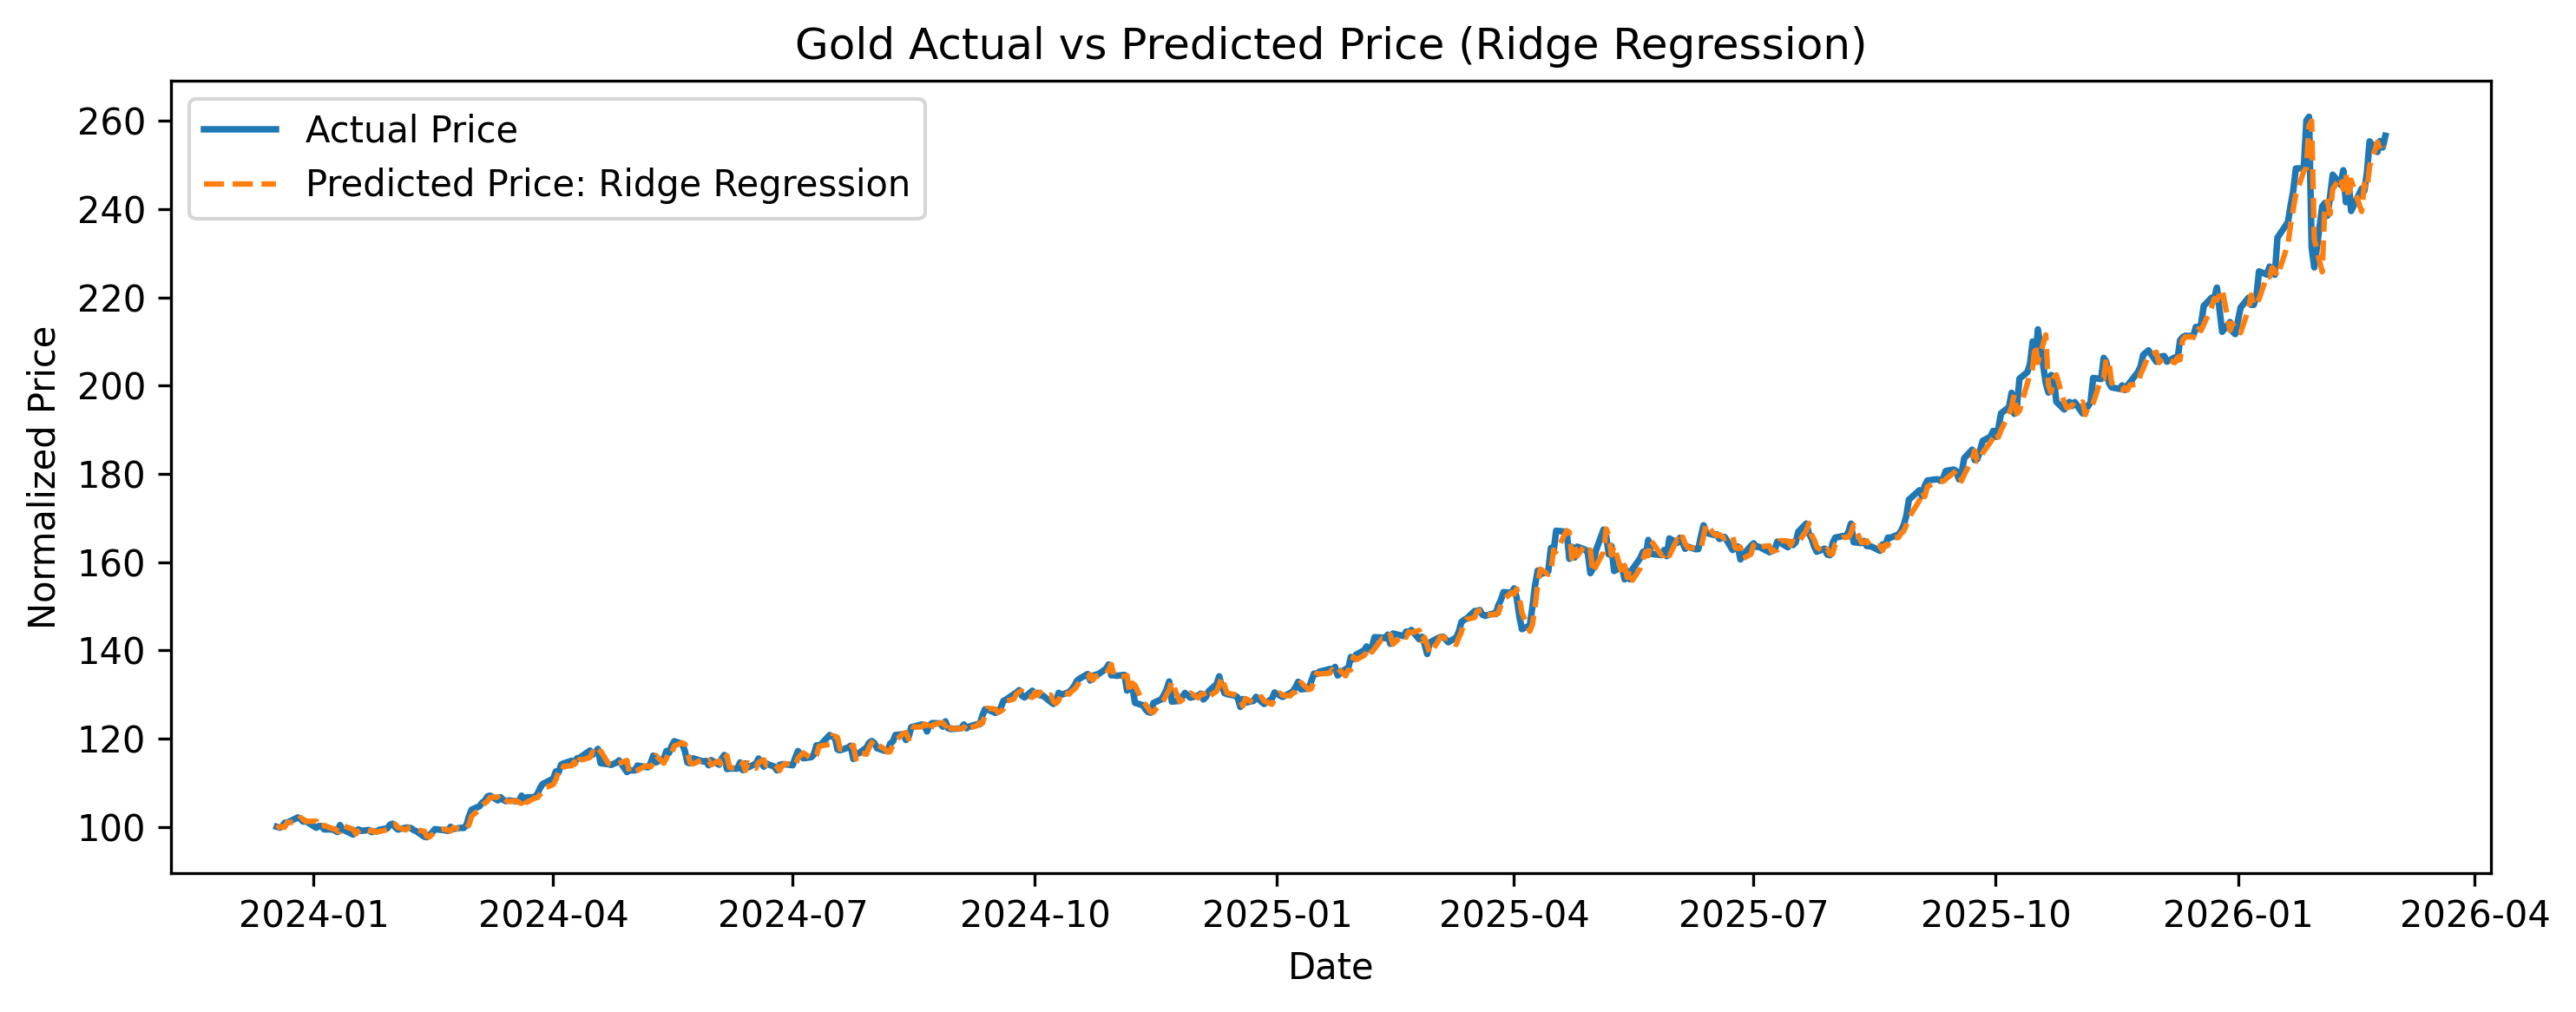
\includegraphics[width=\textwidth, trim=0 6 0 6, clip]{modeling_plot/Gold_Ridge_Regression_price_prediction.png}
        \caption{Gold -- Ridge}
    \end{subfigure}
    \hspace{0.025\textwidth}
    \begin{subfigure}[t]{0.29\textwidth}
        \centering
        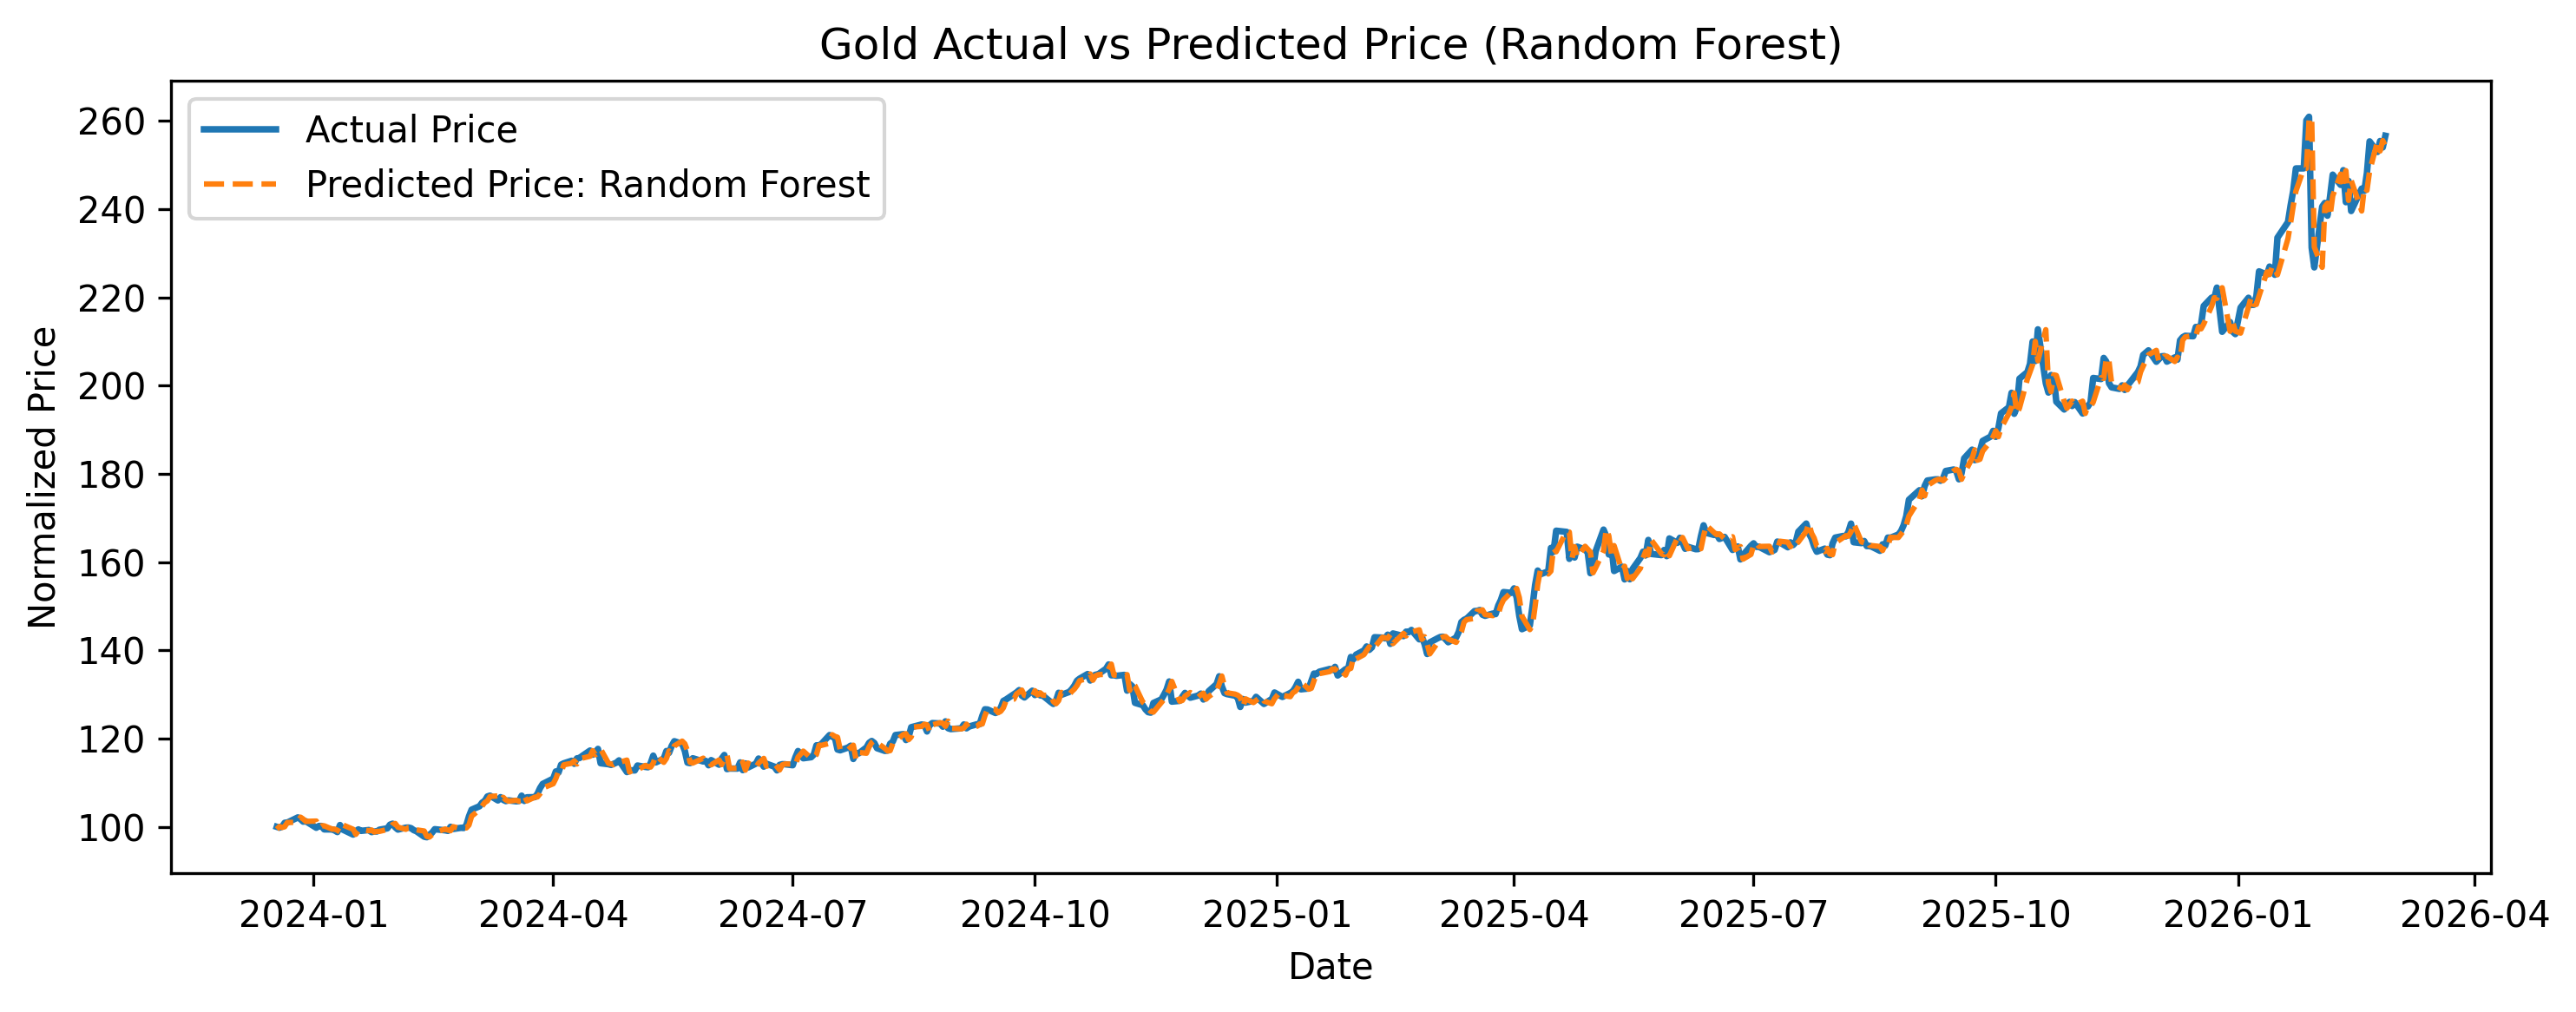
\includegraphics[width=\textwidth, trim=0 6 0 6, clip]{modeling_plot/Gold_Random_Forest_price_prediction.png}
        \caption{Gold -- RF}
    \end{subfigure}
    \hspace{0.025\textwidth}
    \begin{subfigure}[t]{0.29\textwidth}
        \centering
        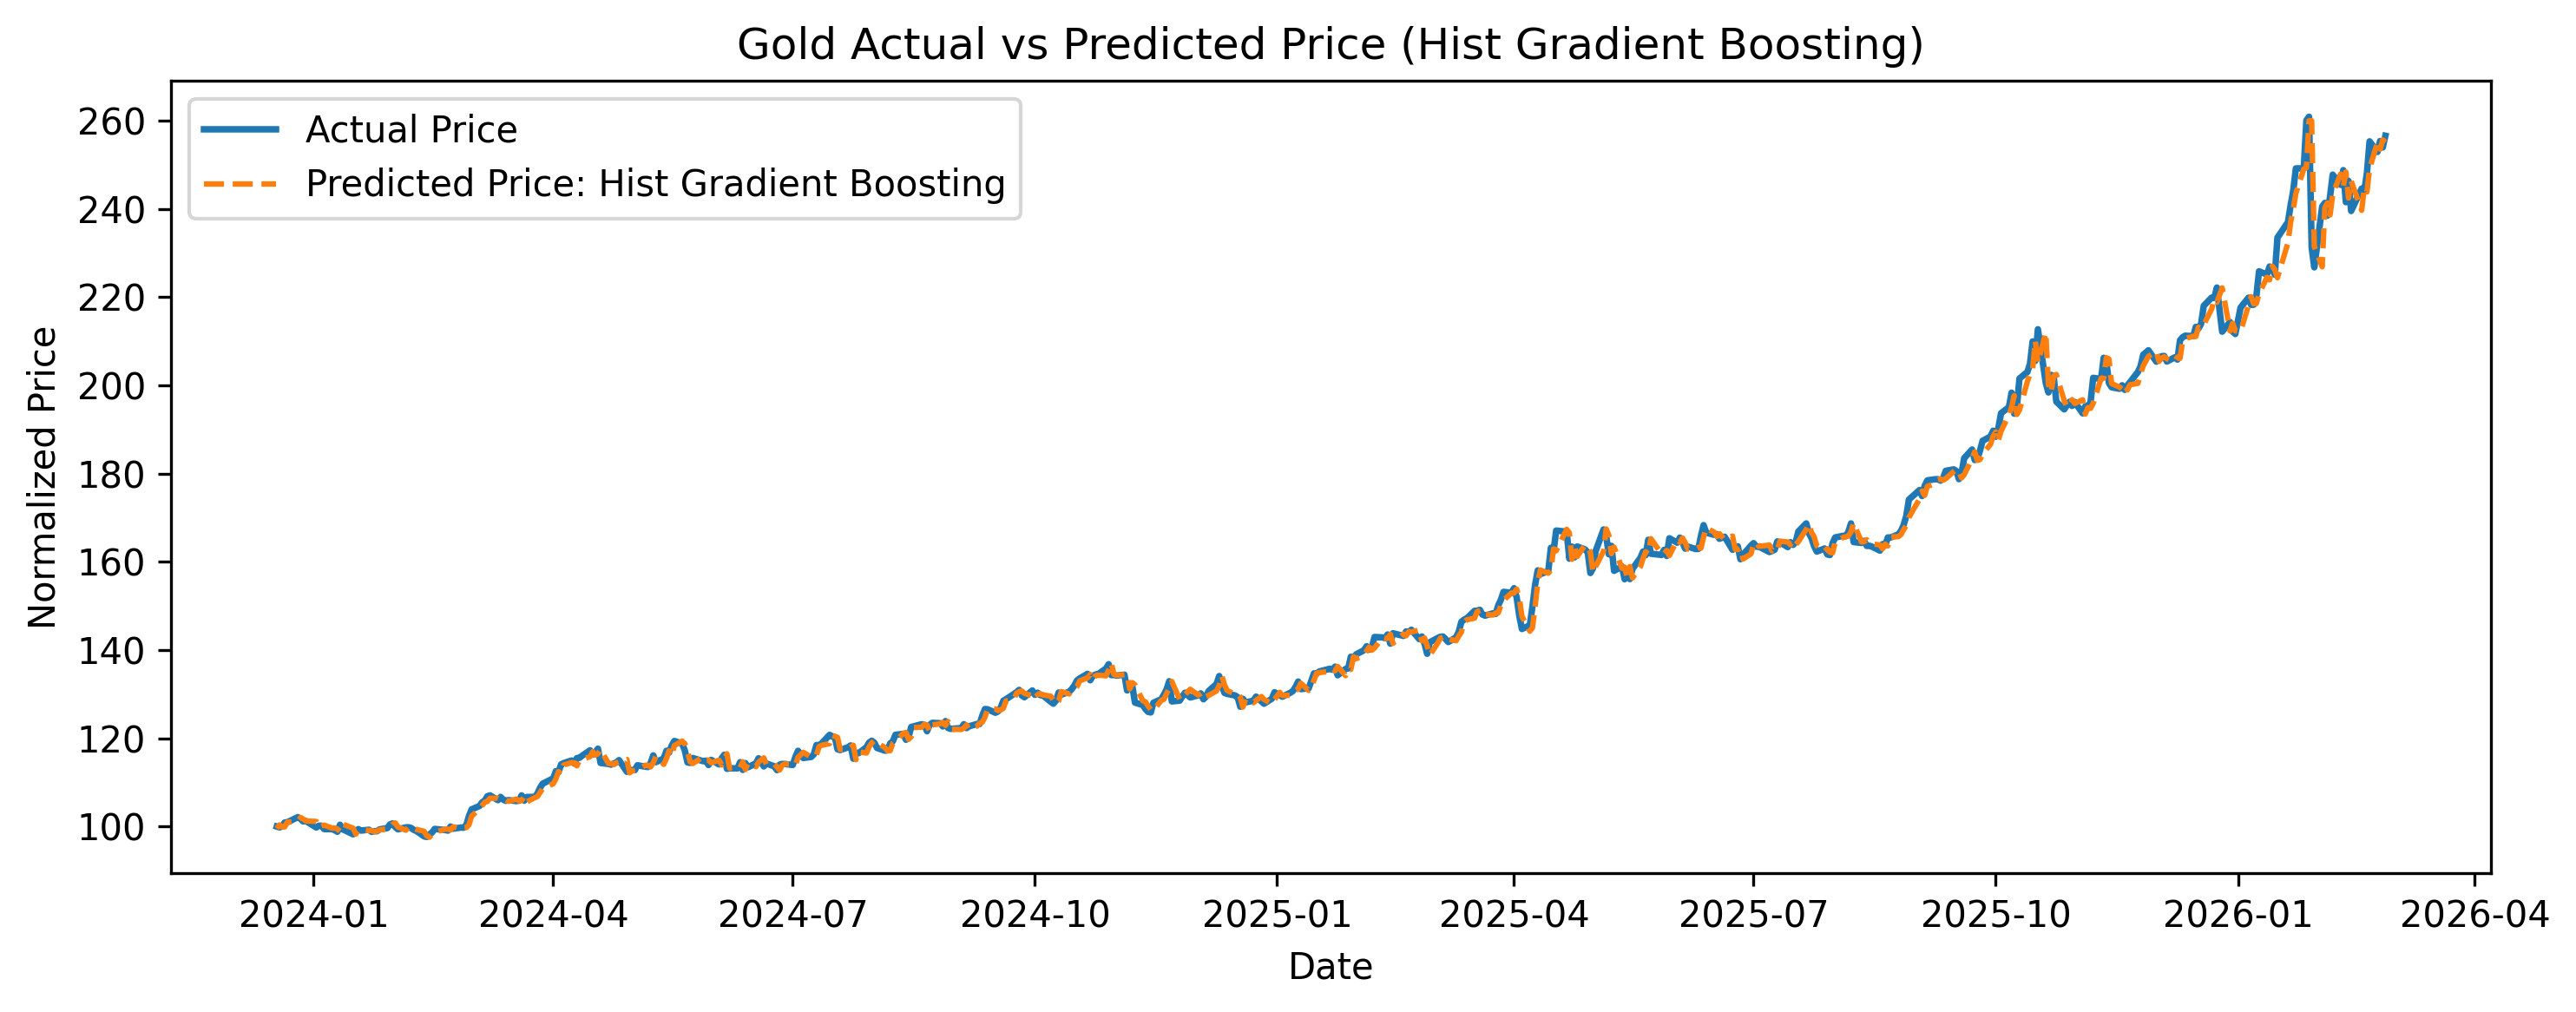
\includegraphics[width=\textwidth, trim=0 6 0 6, clip]{modeling_plot/Gold_Hist_Gradient_Boosting_price_prediction.png}
        \caption{Gold -- HGB}
    \end{subfigure}

    \vspace{0.20cm}

    % ---------------- Silver ----------------
    \begin{subfigure}[t]{0.29\textwidth}
        \centering
        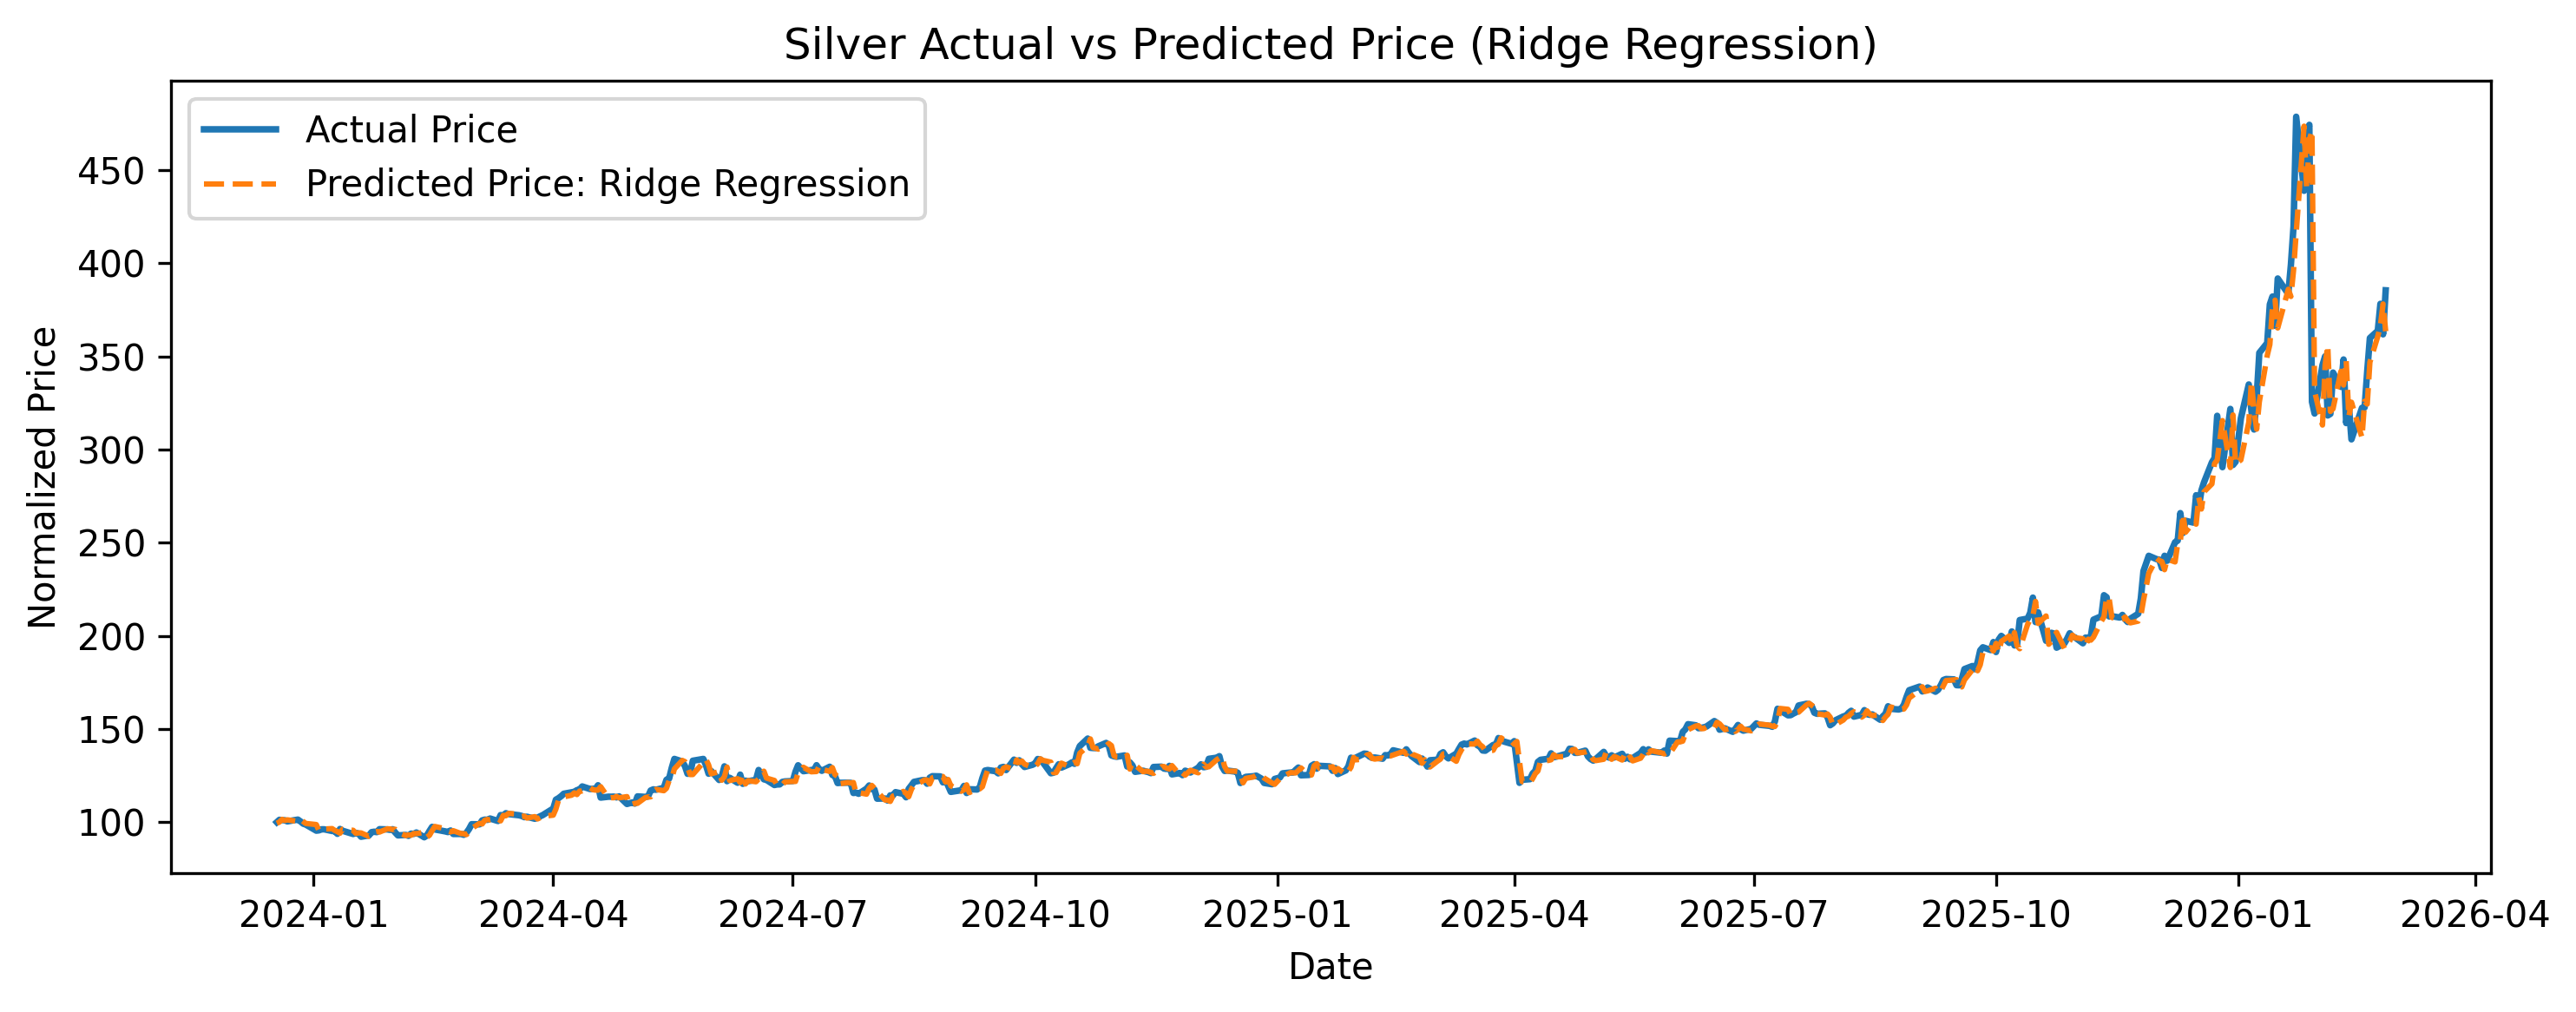
\includegraphics[width=\textwidth, trim=0 6 0 6, clip]{modeling_plot/Silver_Ridge_Regression_price_prediction.png}
        \caption{Silver -- Ridge}
    \end{subfigure}
    \hspace{0.025\textwidth}
    \begin{subfigure}[t]{0.29\textwidth}
        \centering
        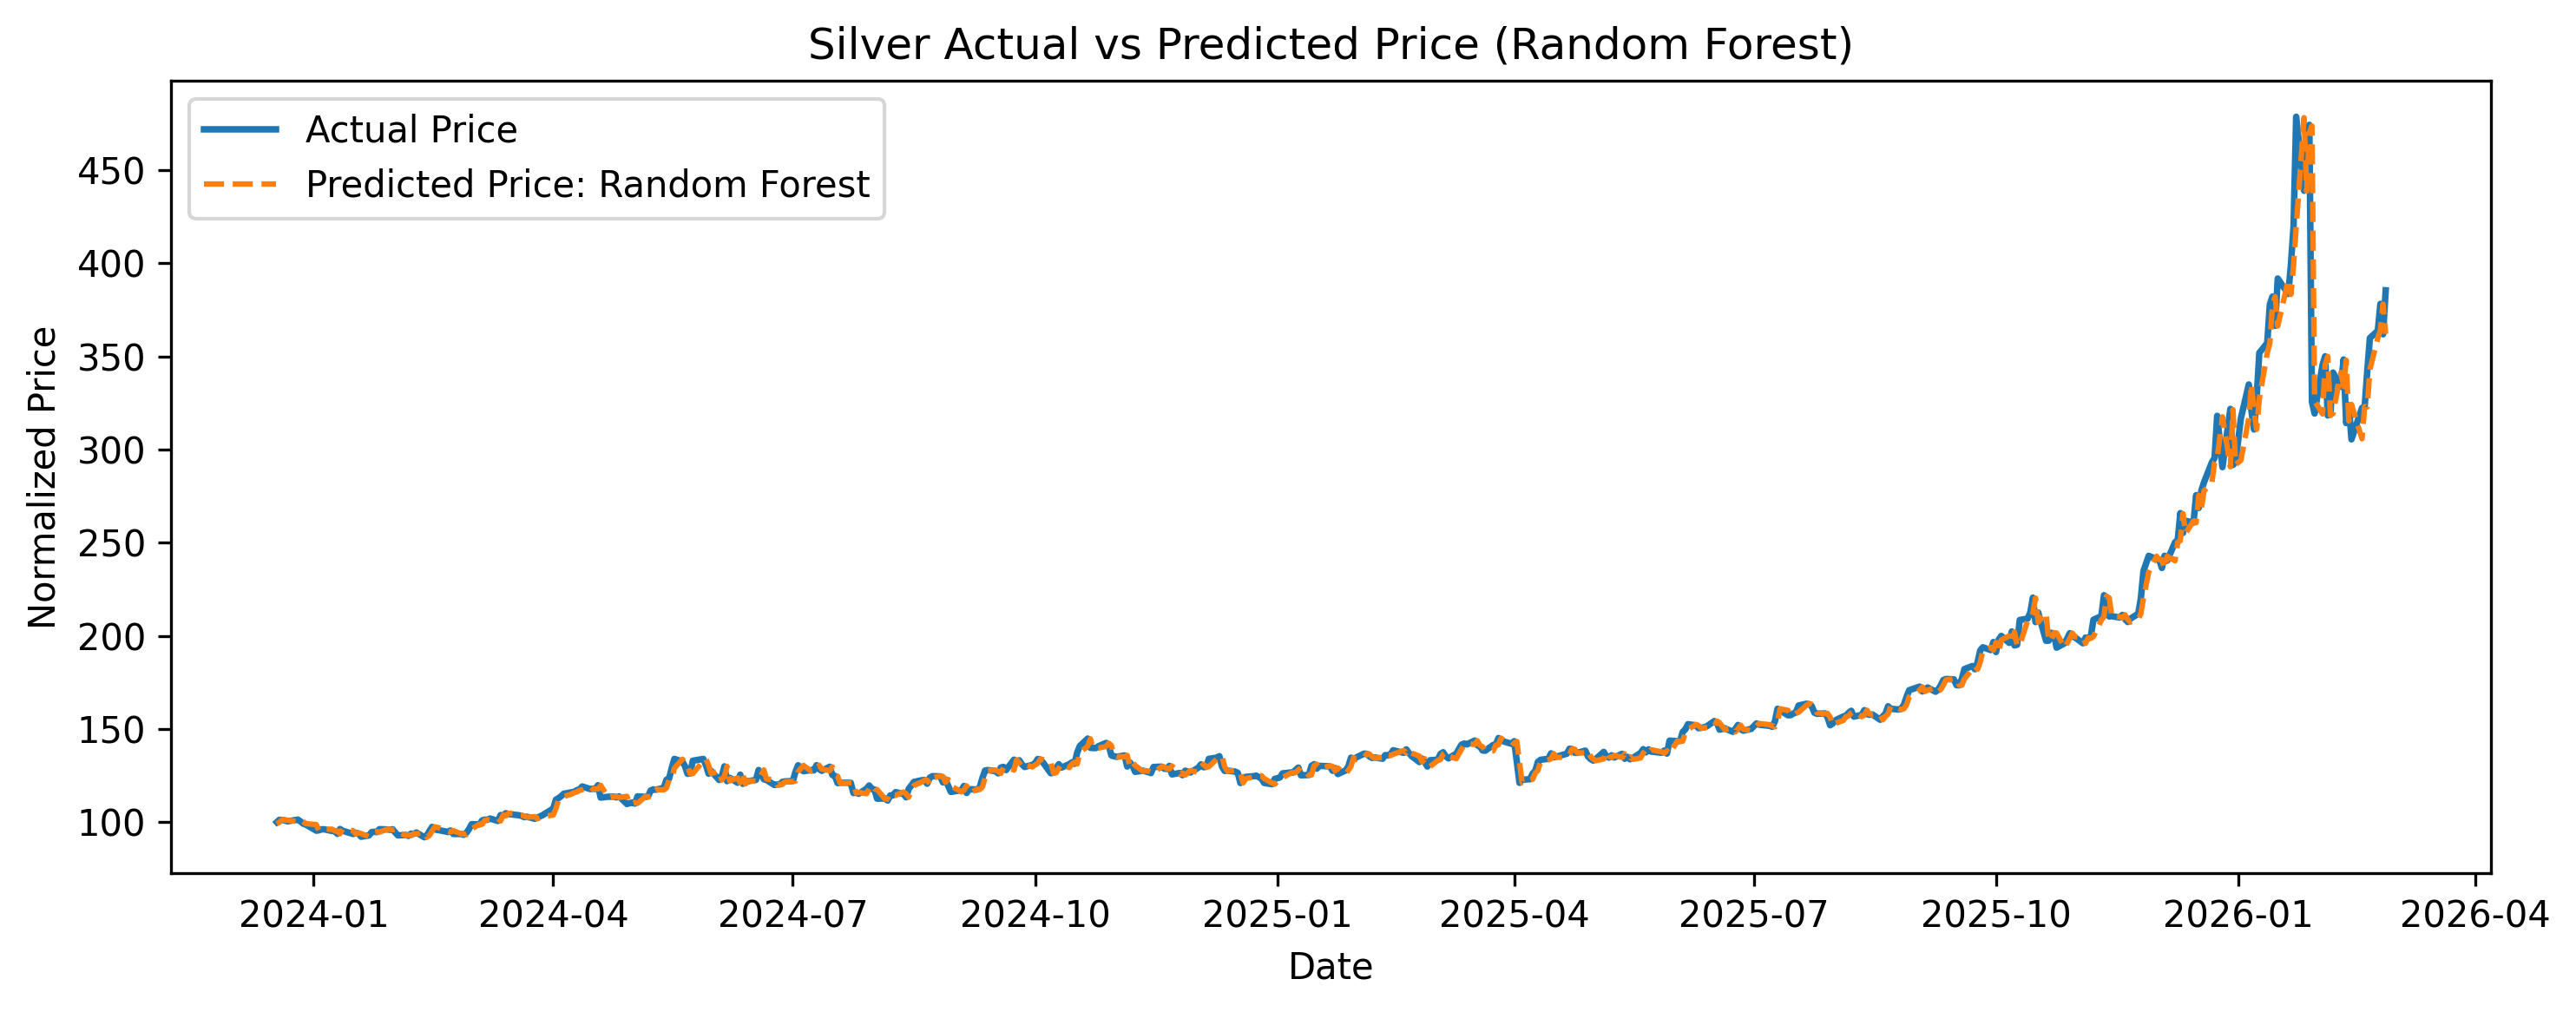
\includegraphics[width=\textwidth, trim=0 6 0 6, clip]{modeling_plot/Silver_Random_Forest_price_prediction.png}
        \caption{Silver -- RF}
    \end{subfigure}
    \hspace{0.025\textwidth}
    \begin{subfigure}[t]{0.29\textwidth}
        \centering
        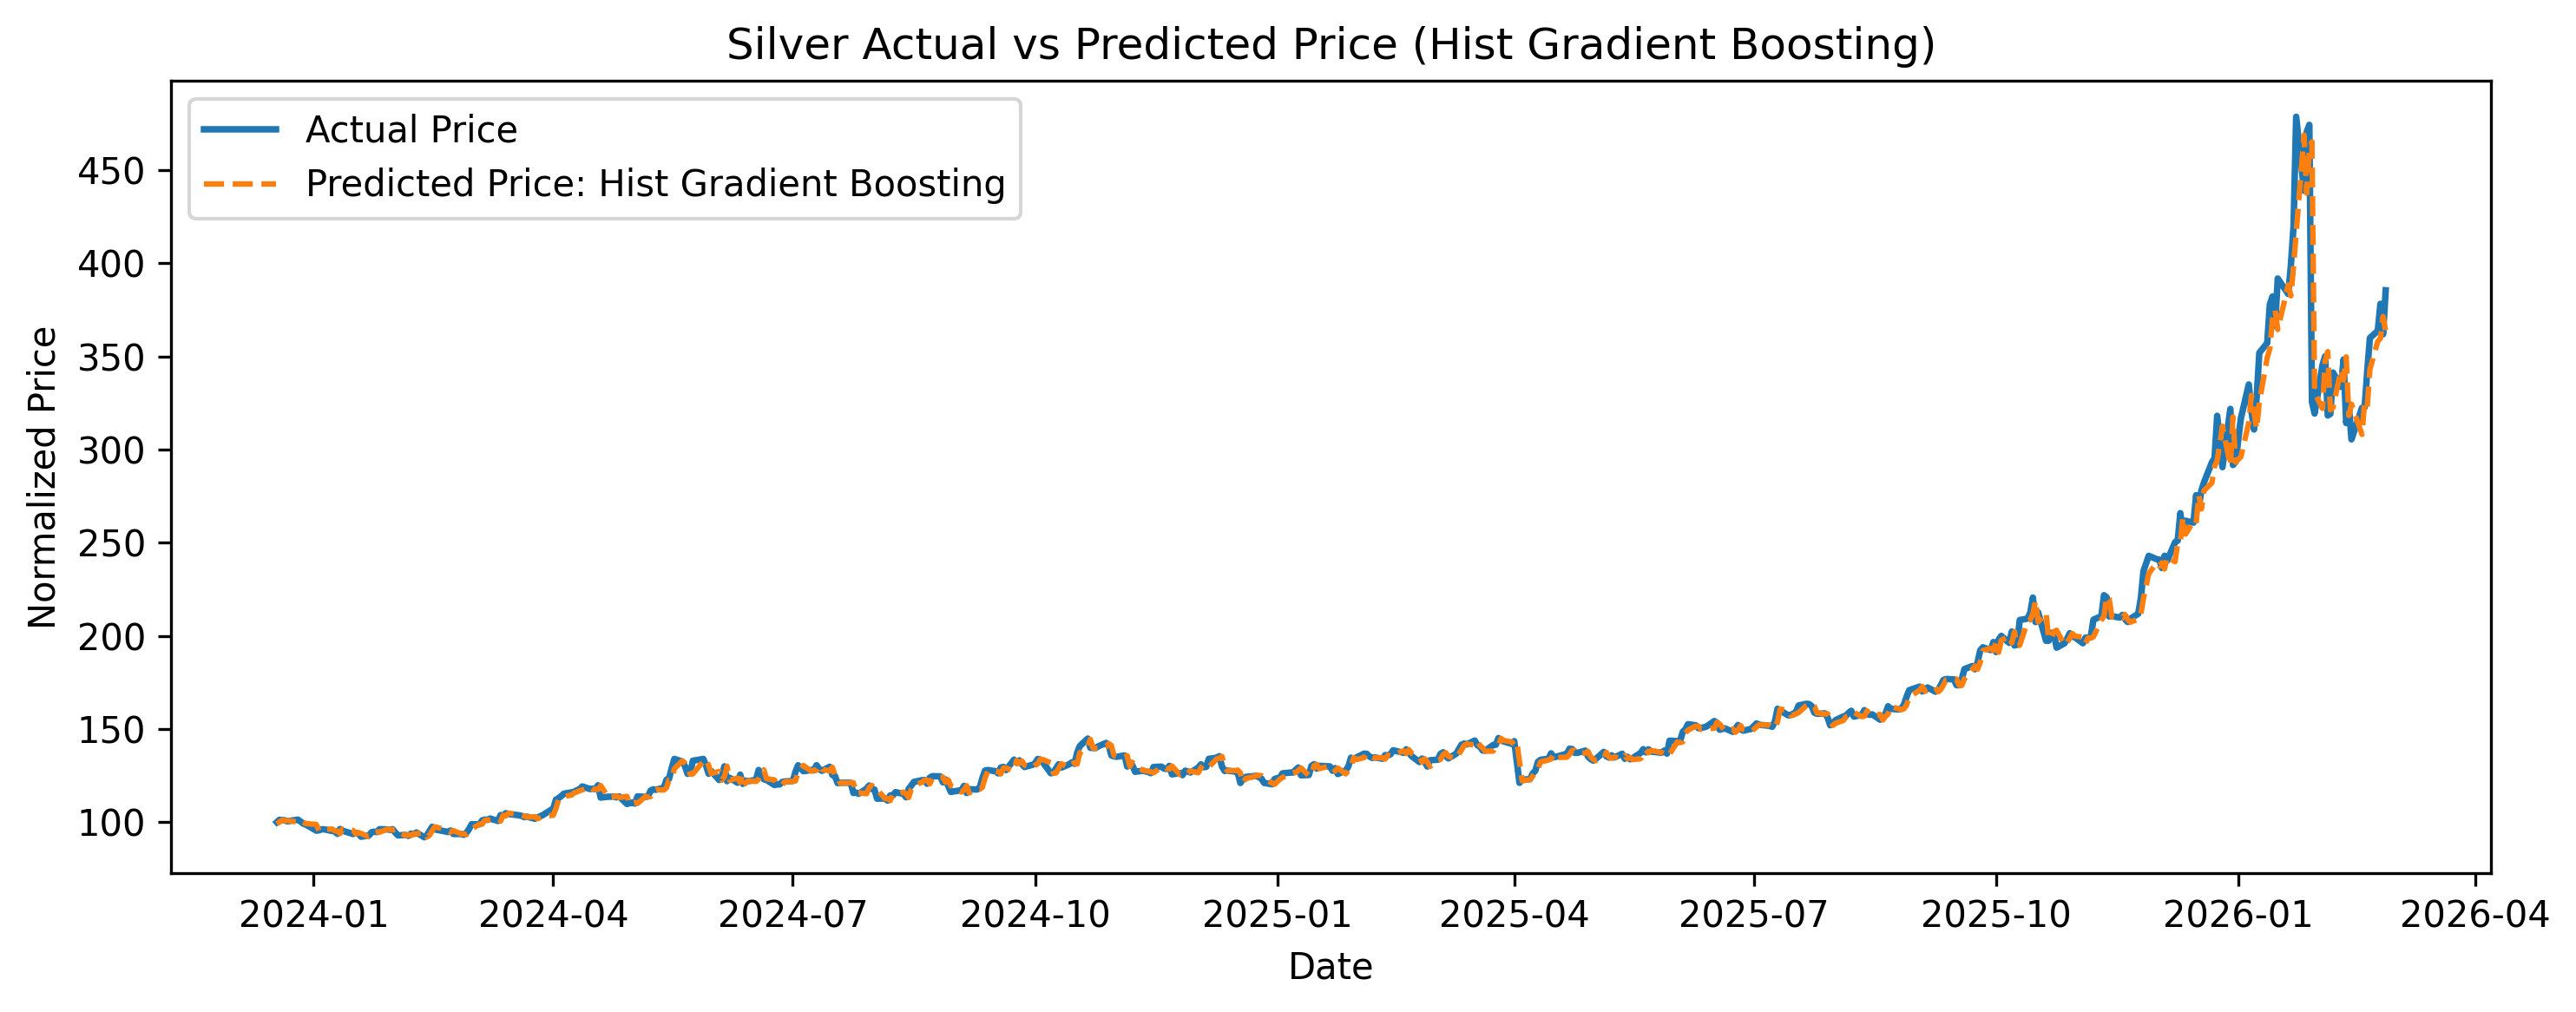
\includegraphics[width=\textwidth, trim=0 6 0 6, clip]{modeling_plot/Silver_Hist_Gradient_Boosting_price_prediction.png}
        \caption{Silver -- HGB}
    \end{subfigure}

    \vspace{0.12cm}
    \caption{Actual vs Predicted Prices for Precious Metals}
    \label{fig:price_predictions_metals}
\end{figure}

\vspace{0.60cm}

% ------------------------------------------------------------
% Figure: USD Index and WTI Oil
% ------------------------------------------------------------

\begin{figure}[H]
    \centering
    \captionsetup[subfigure]{skip=4pt}
    \setlength{\abovecaptionskip}{5pt}
    \setlength{\belowcaptionskip}{3pt}

    % ---------------- USD Index ----------------
    \begin{subfigure}[t]{0.29\textwidth}
        \centering
        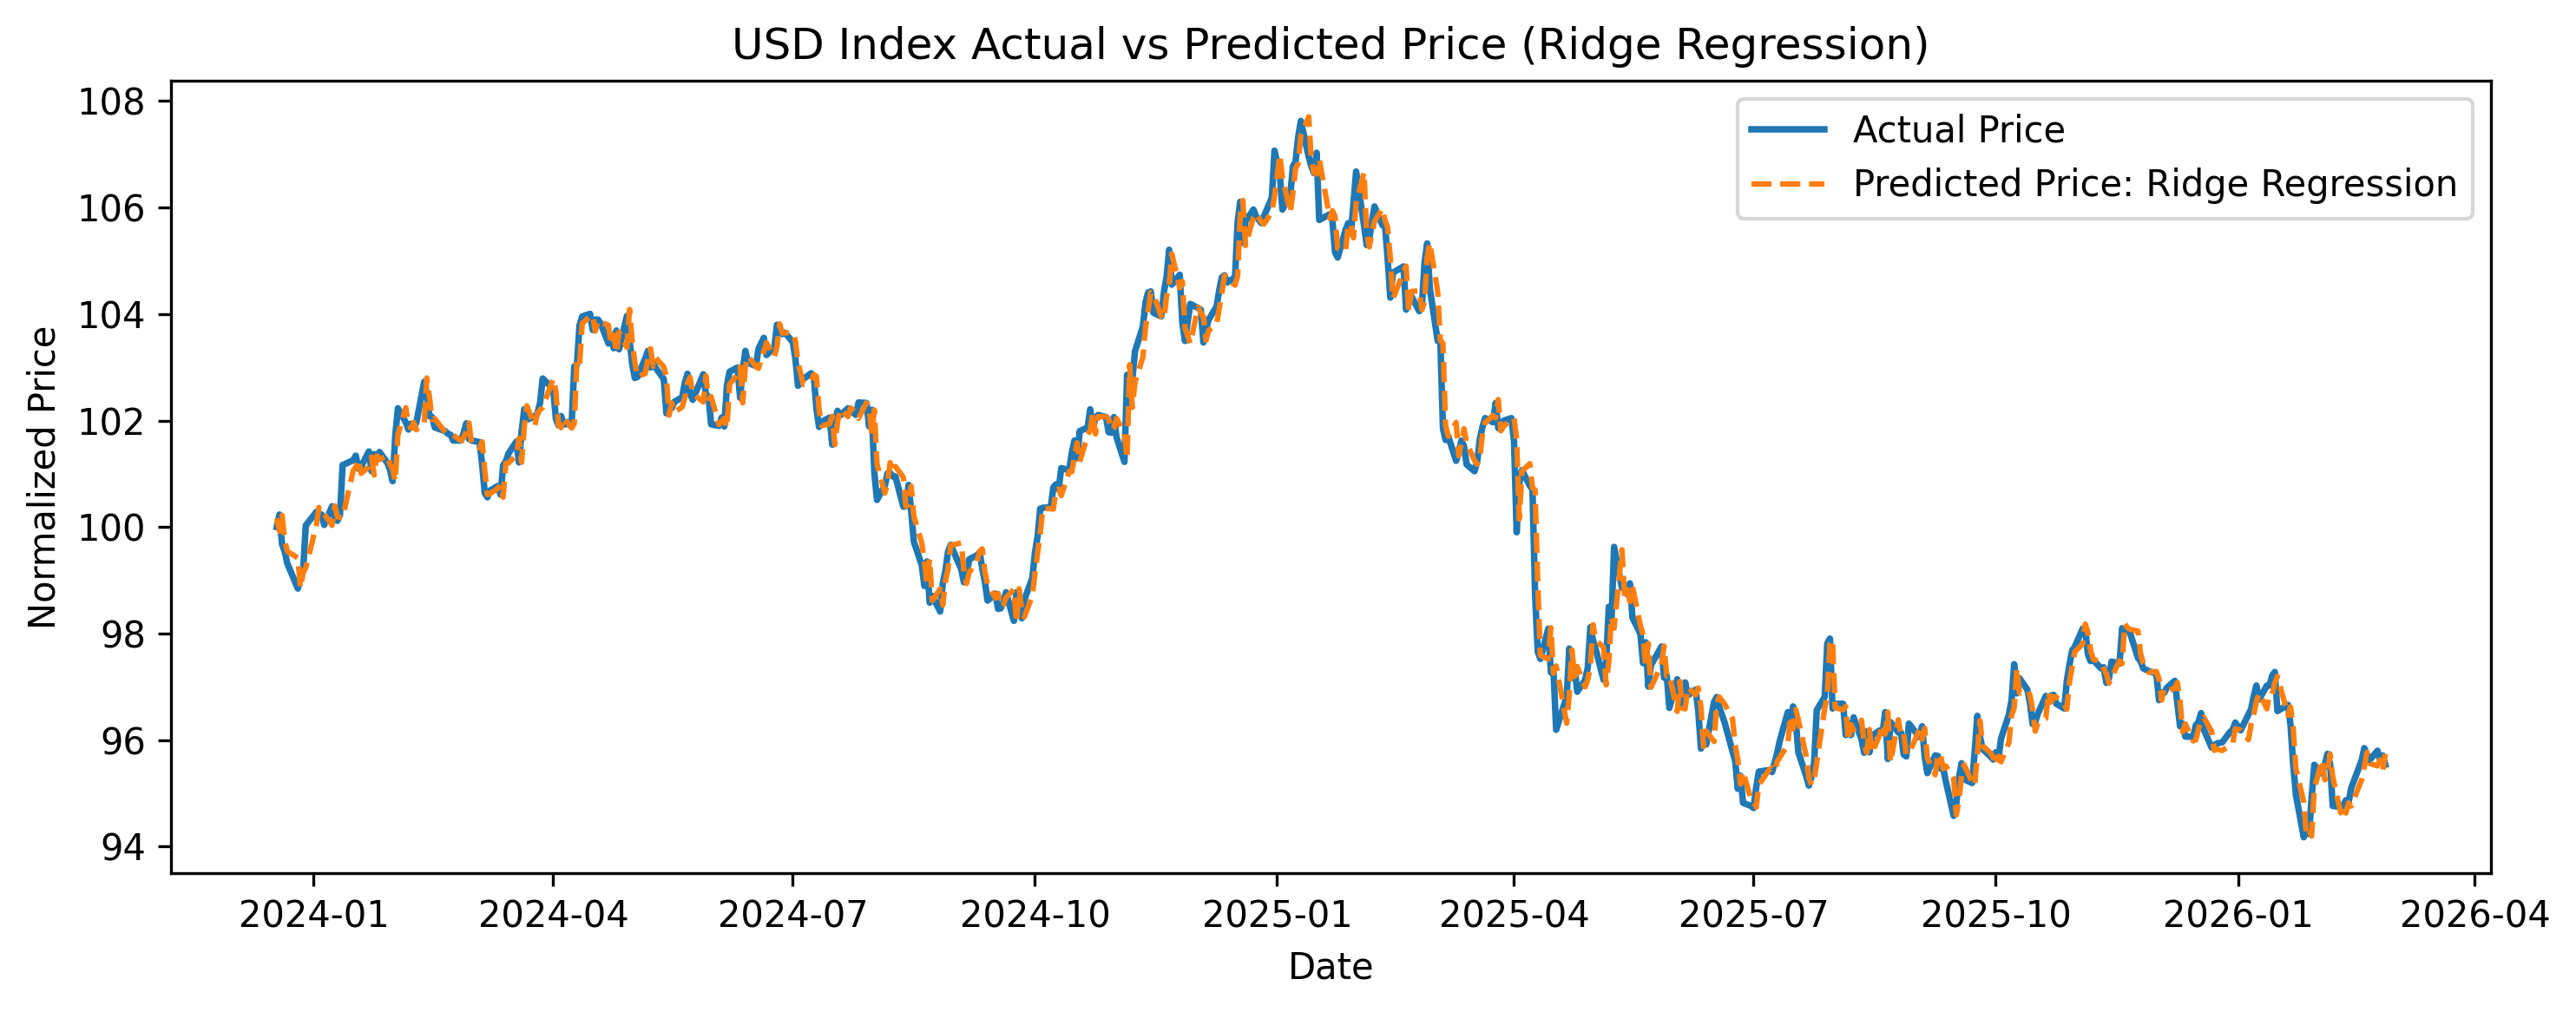
\includegraphics[width=\textwidth, trim=0 6 0 6, clip]{modeling_plot/USD_Index_Ridge_Regression_price_prediction.png}
        \caption{USD Index -- Ridge}
    \end{subfigure}
    \hspace{0.025\textwidth}
    \begin{subfigure}[t]{0.29\textwidth}
        \centering
        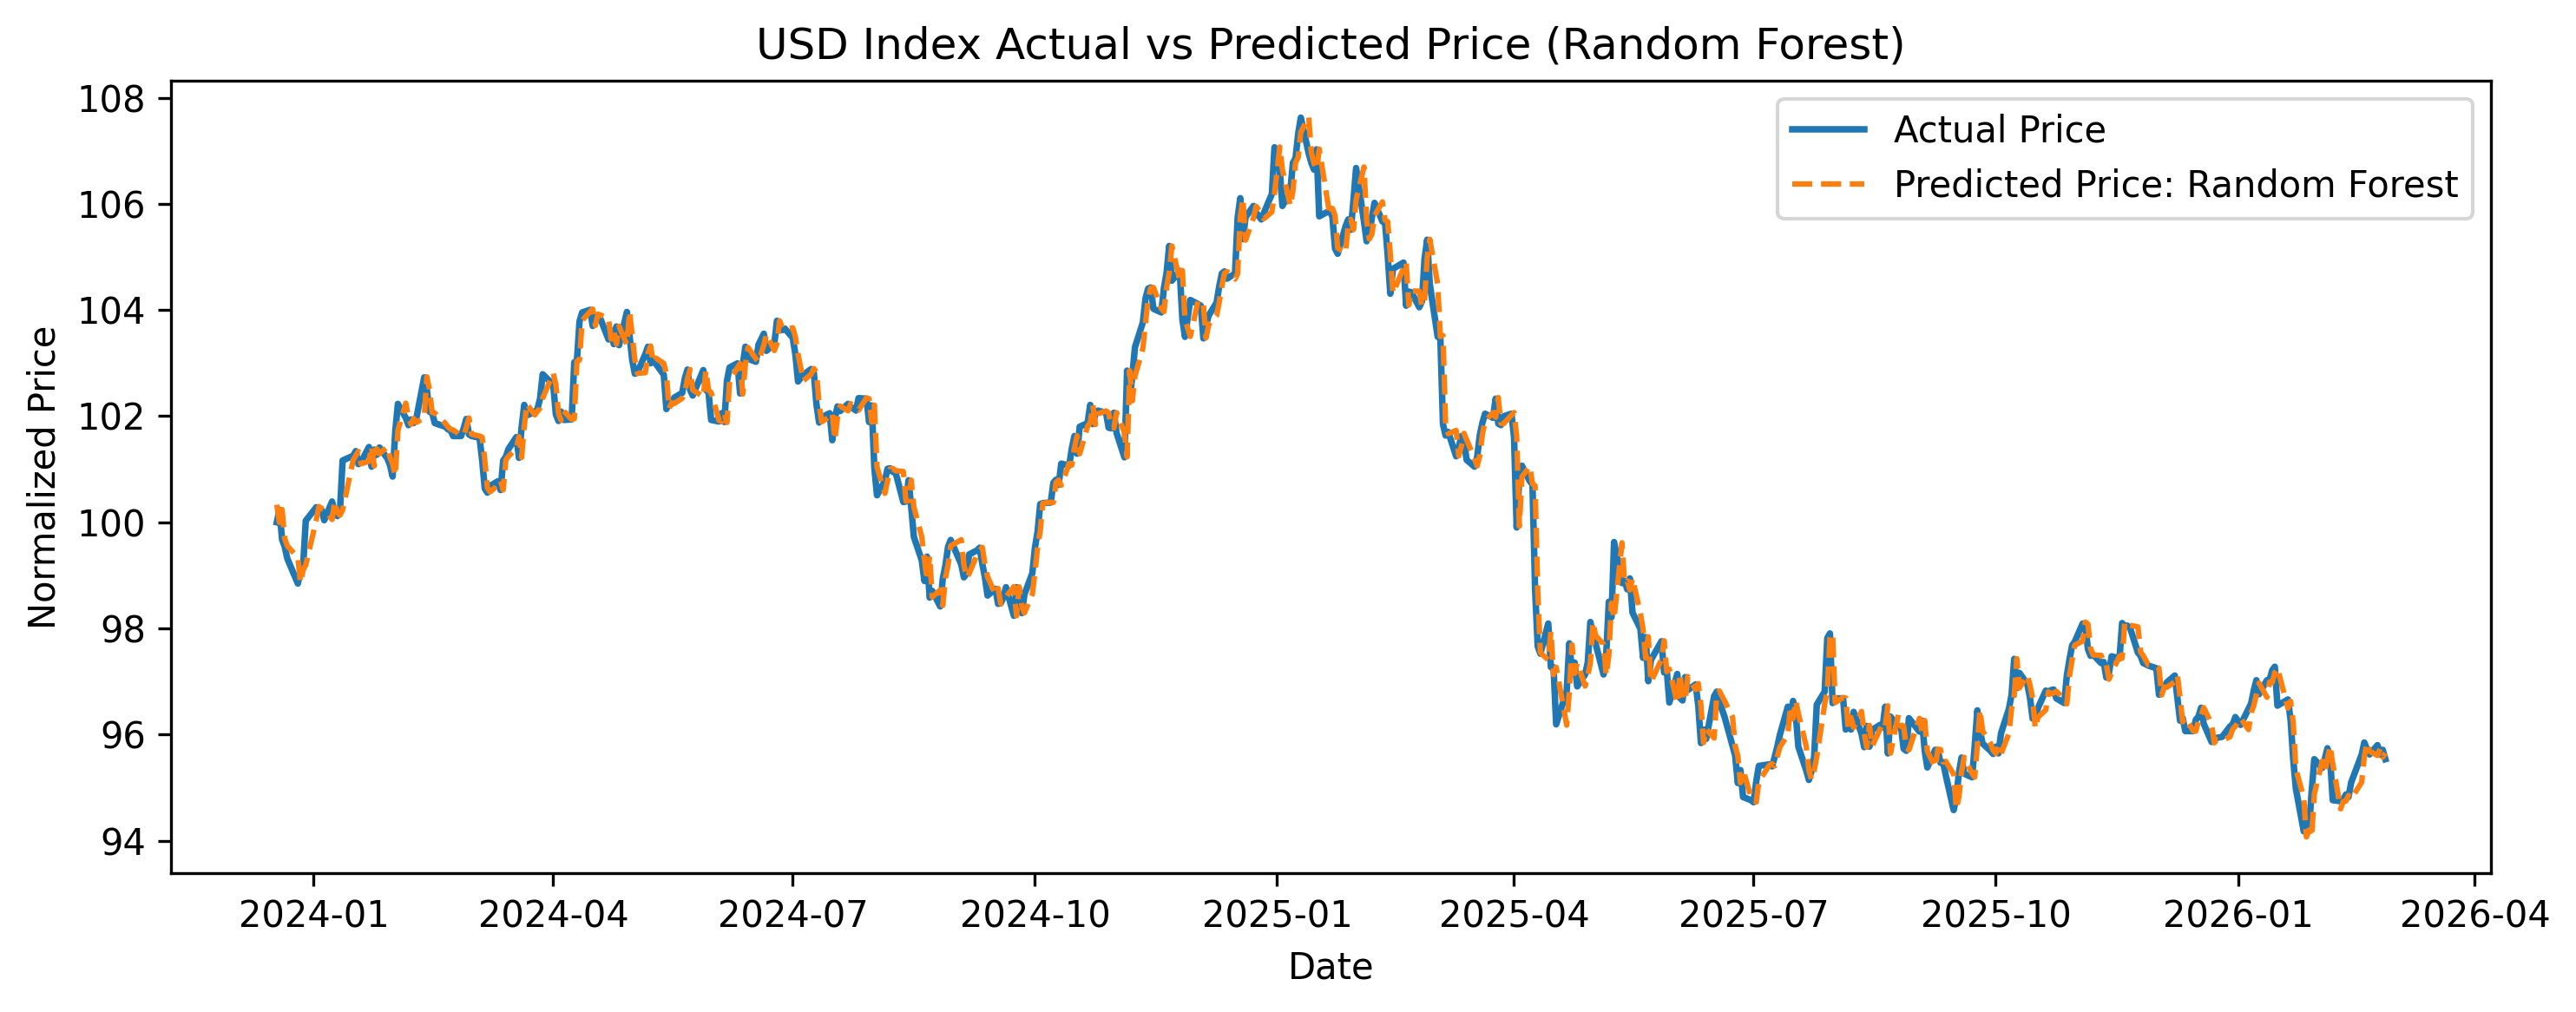
\includegraphics[width=\textwidth, trim=0 6 0 6, clip]{modeling_plot/USD_Index_Random_Forest_price_prediction.png}
        \caption{USD Index -- RF}
    \end{subfigure}
    \hspace{0.025\textwidth}
    \begin{subfigure}[t]{0.29\textwidth}
        \centering
        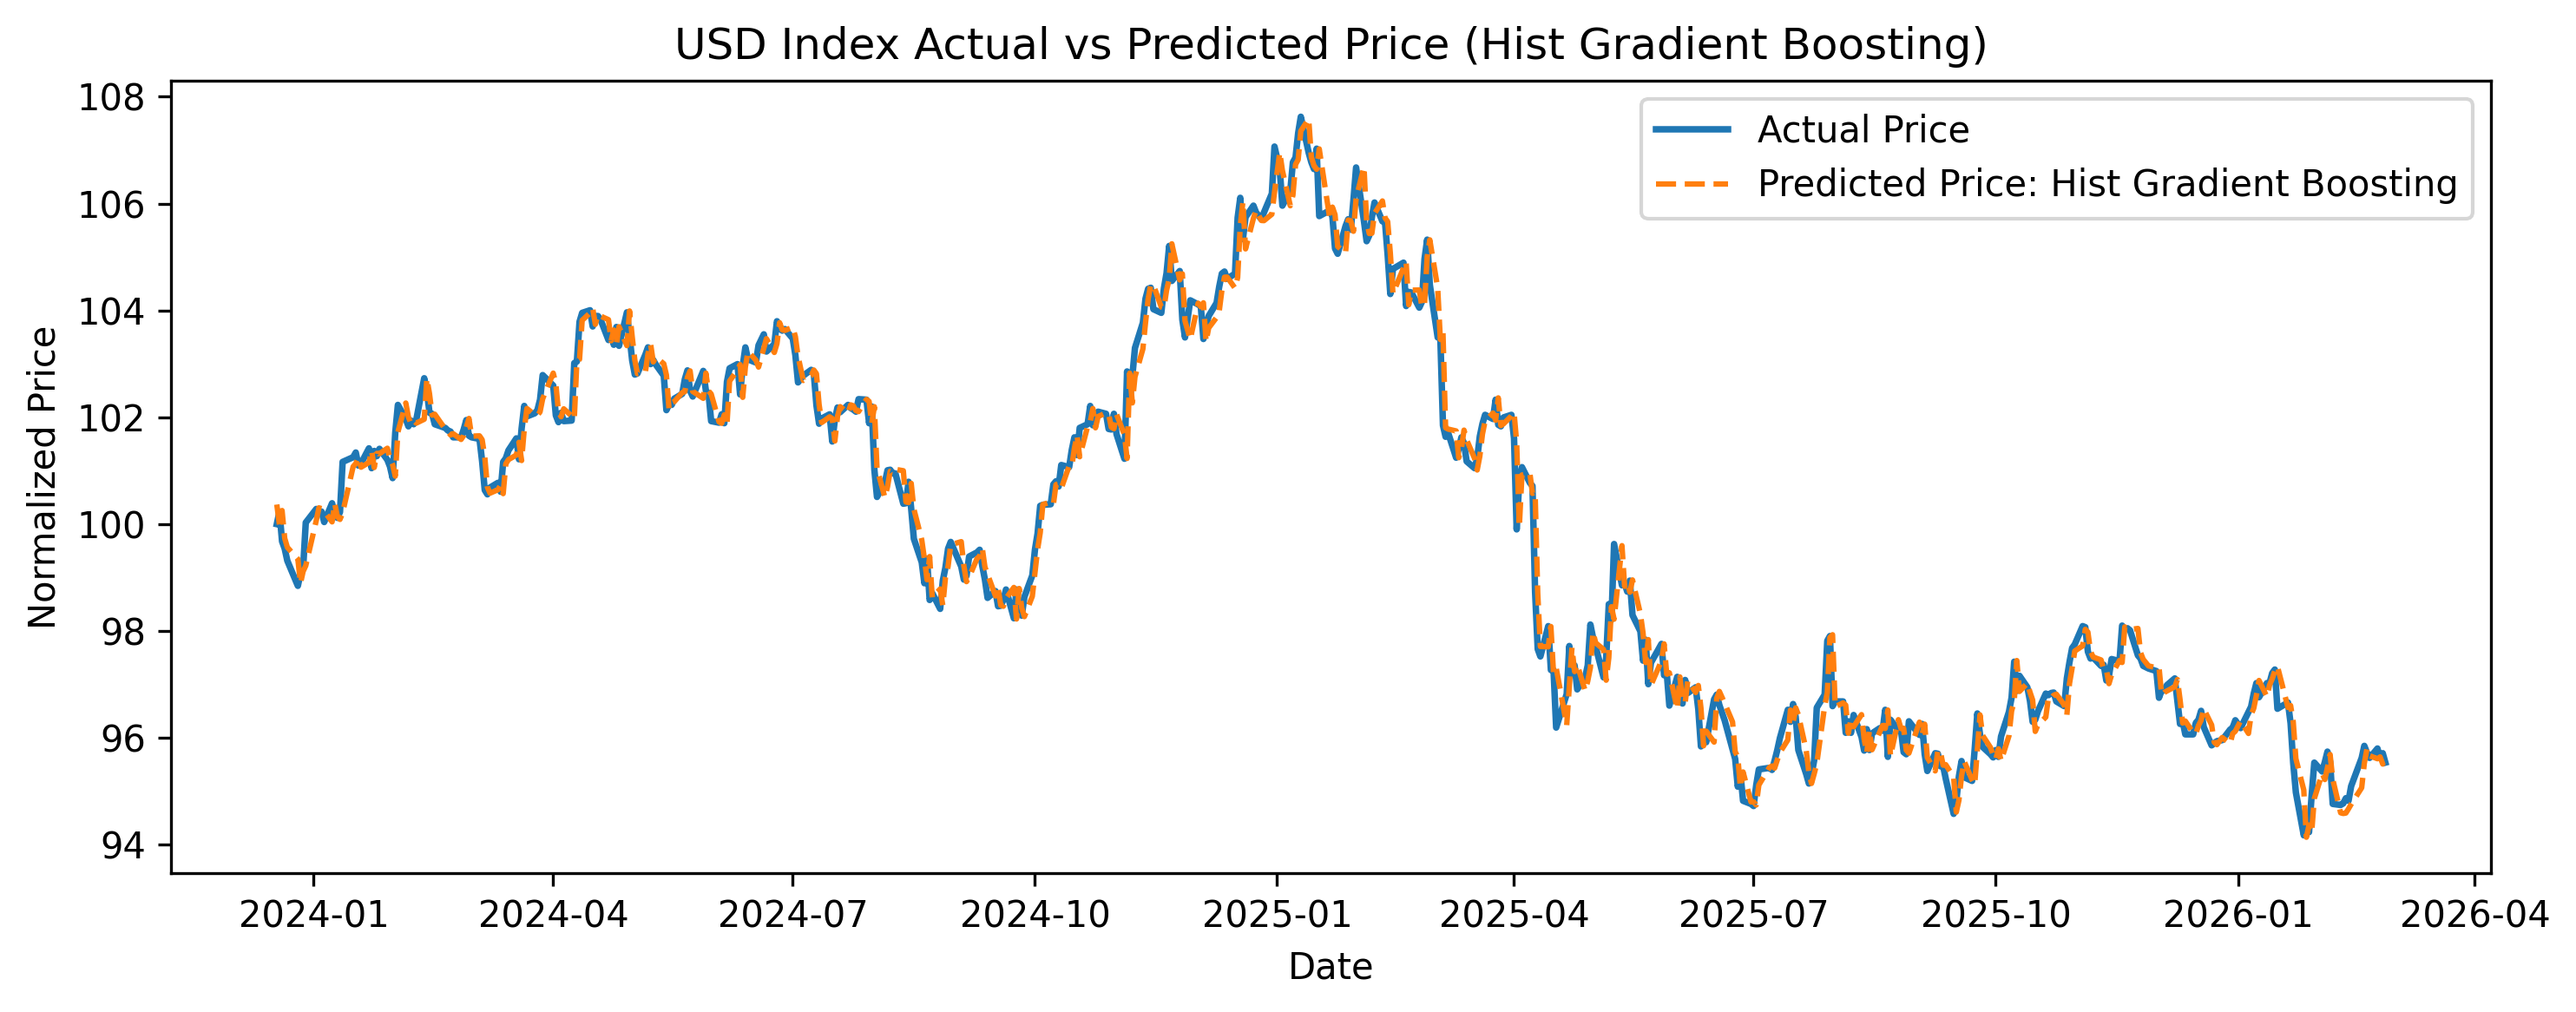
\includegraphics[width=\textwidth, trim=0 6 0 6, clip]{modeling_plot/USD_Index_Hist_Gradient_Boosting_price_prediction.png}
        \caption{USD Index -- HGB}
    \end{subfigure}

    \vspace{0.20cm}

    % ---------------- WTI Oil ----------------
    \begin{subfigure}[t]{0.29\textwidth}
        \centering
        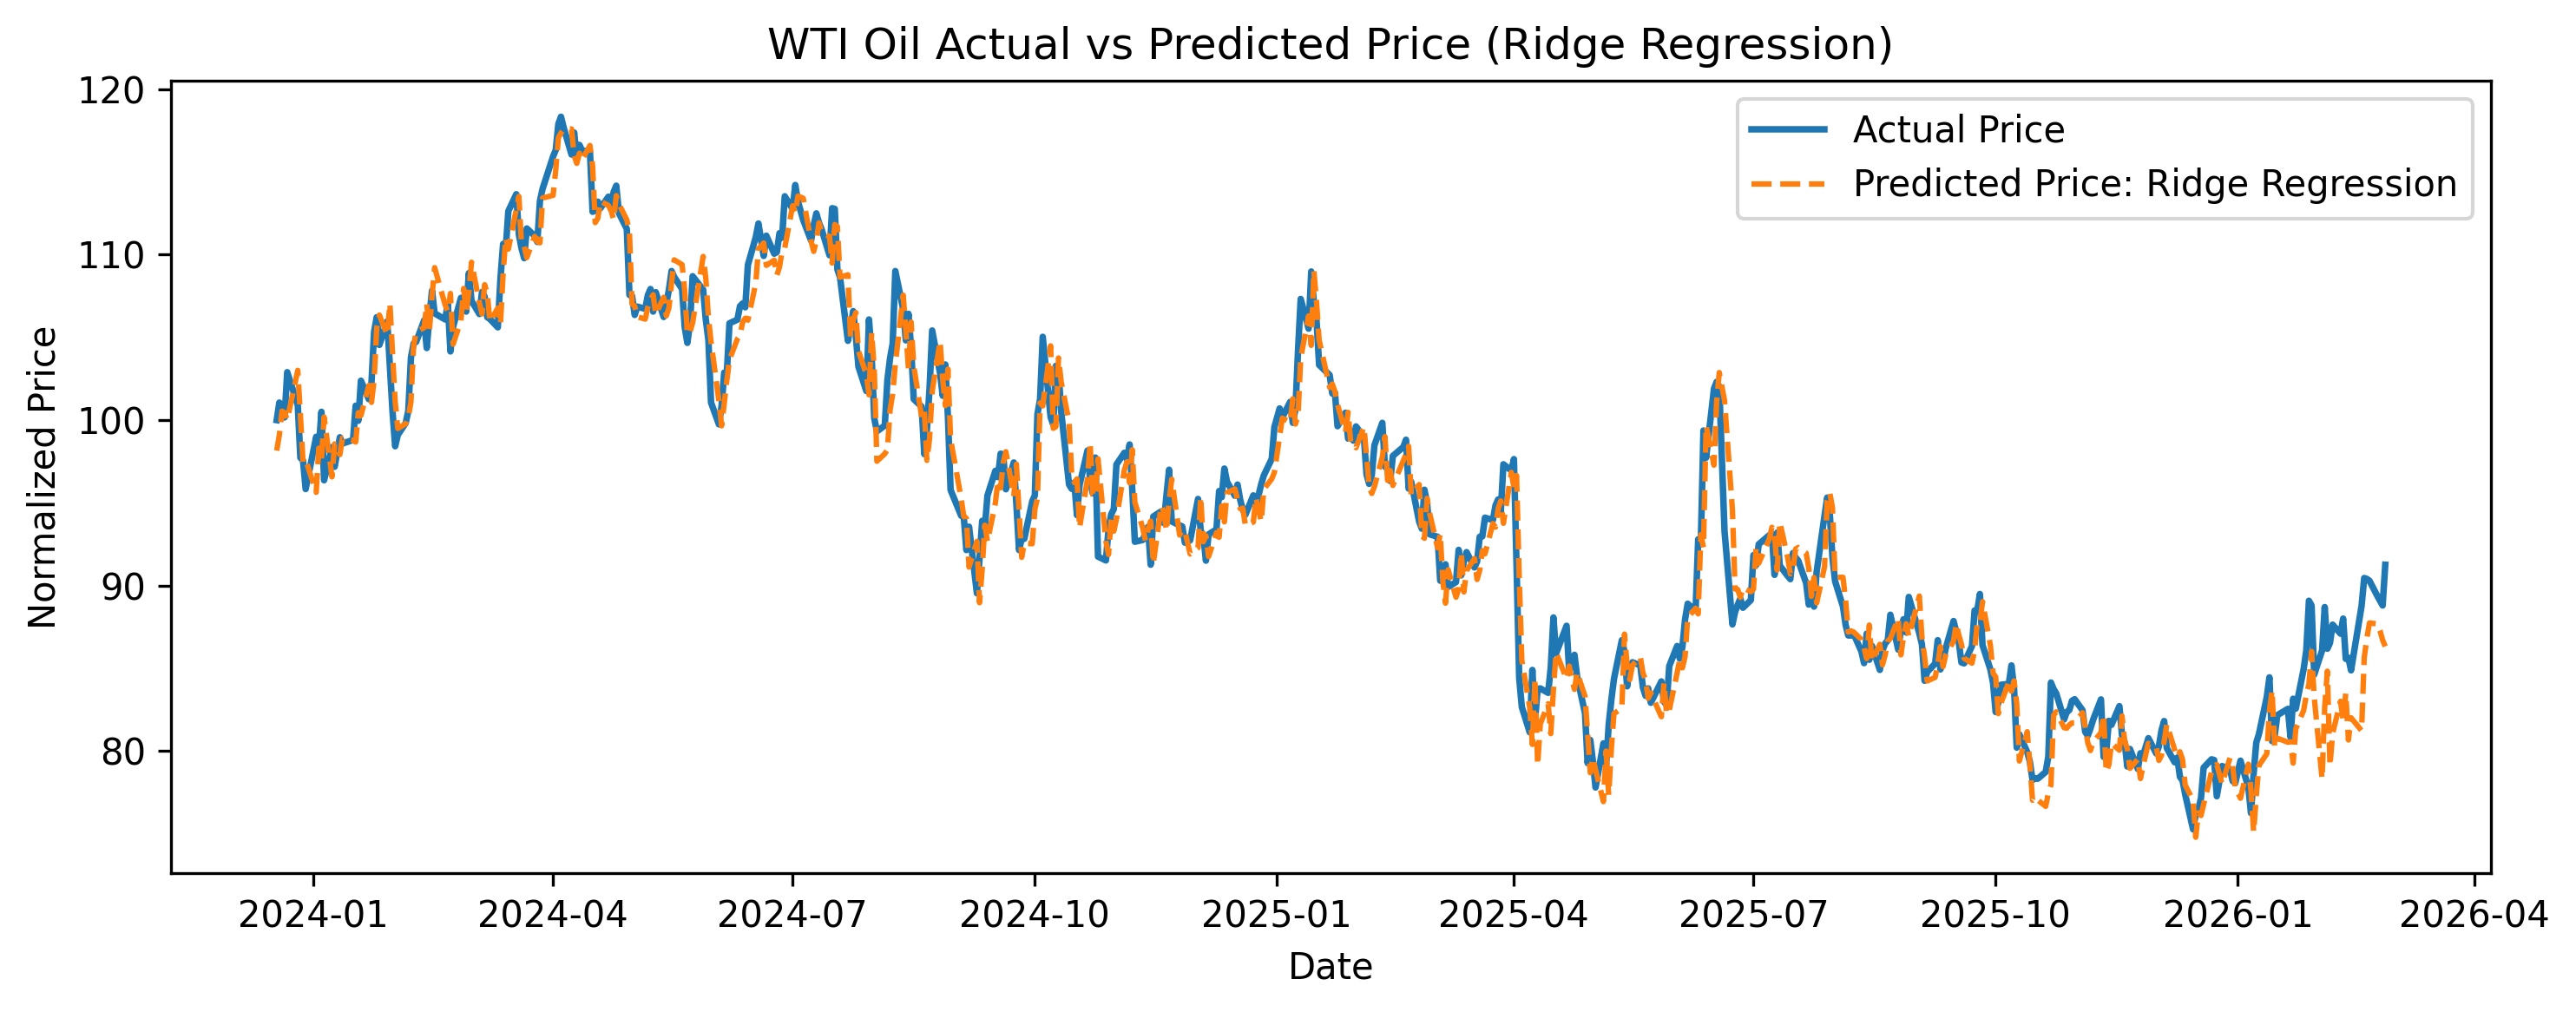
\includegraphics[width=\textwidth, trim=0 6 0 6, clip]{modeling_plot/WTI_Oil_Ridge_Regression_price_prediction.png}
        \caption{WTI Oil -- Ridge}
    \end{subfigure}
    \hspace{0.025\textwidth}
    \begin{subfigure}[t]{0.29\textwidth}
        \centering
        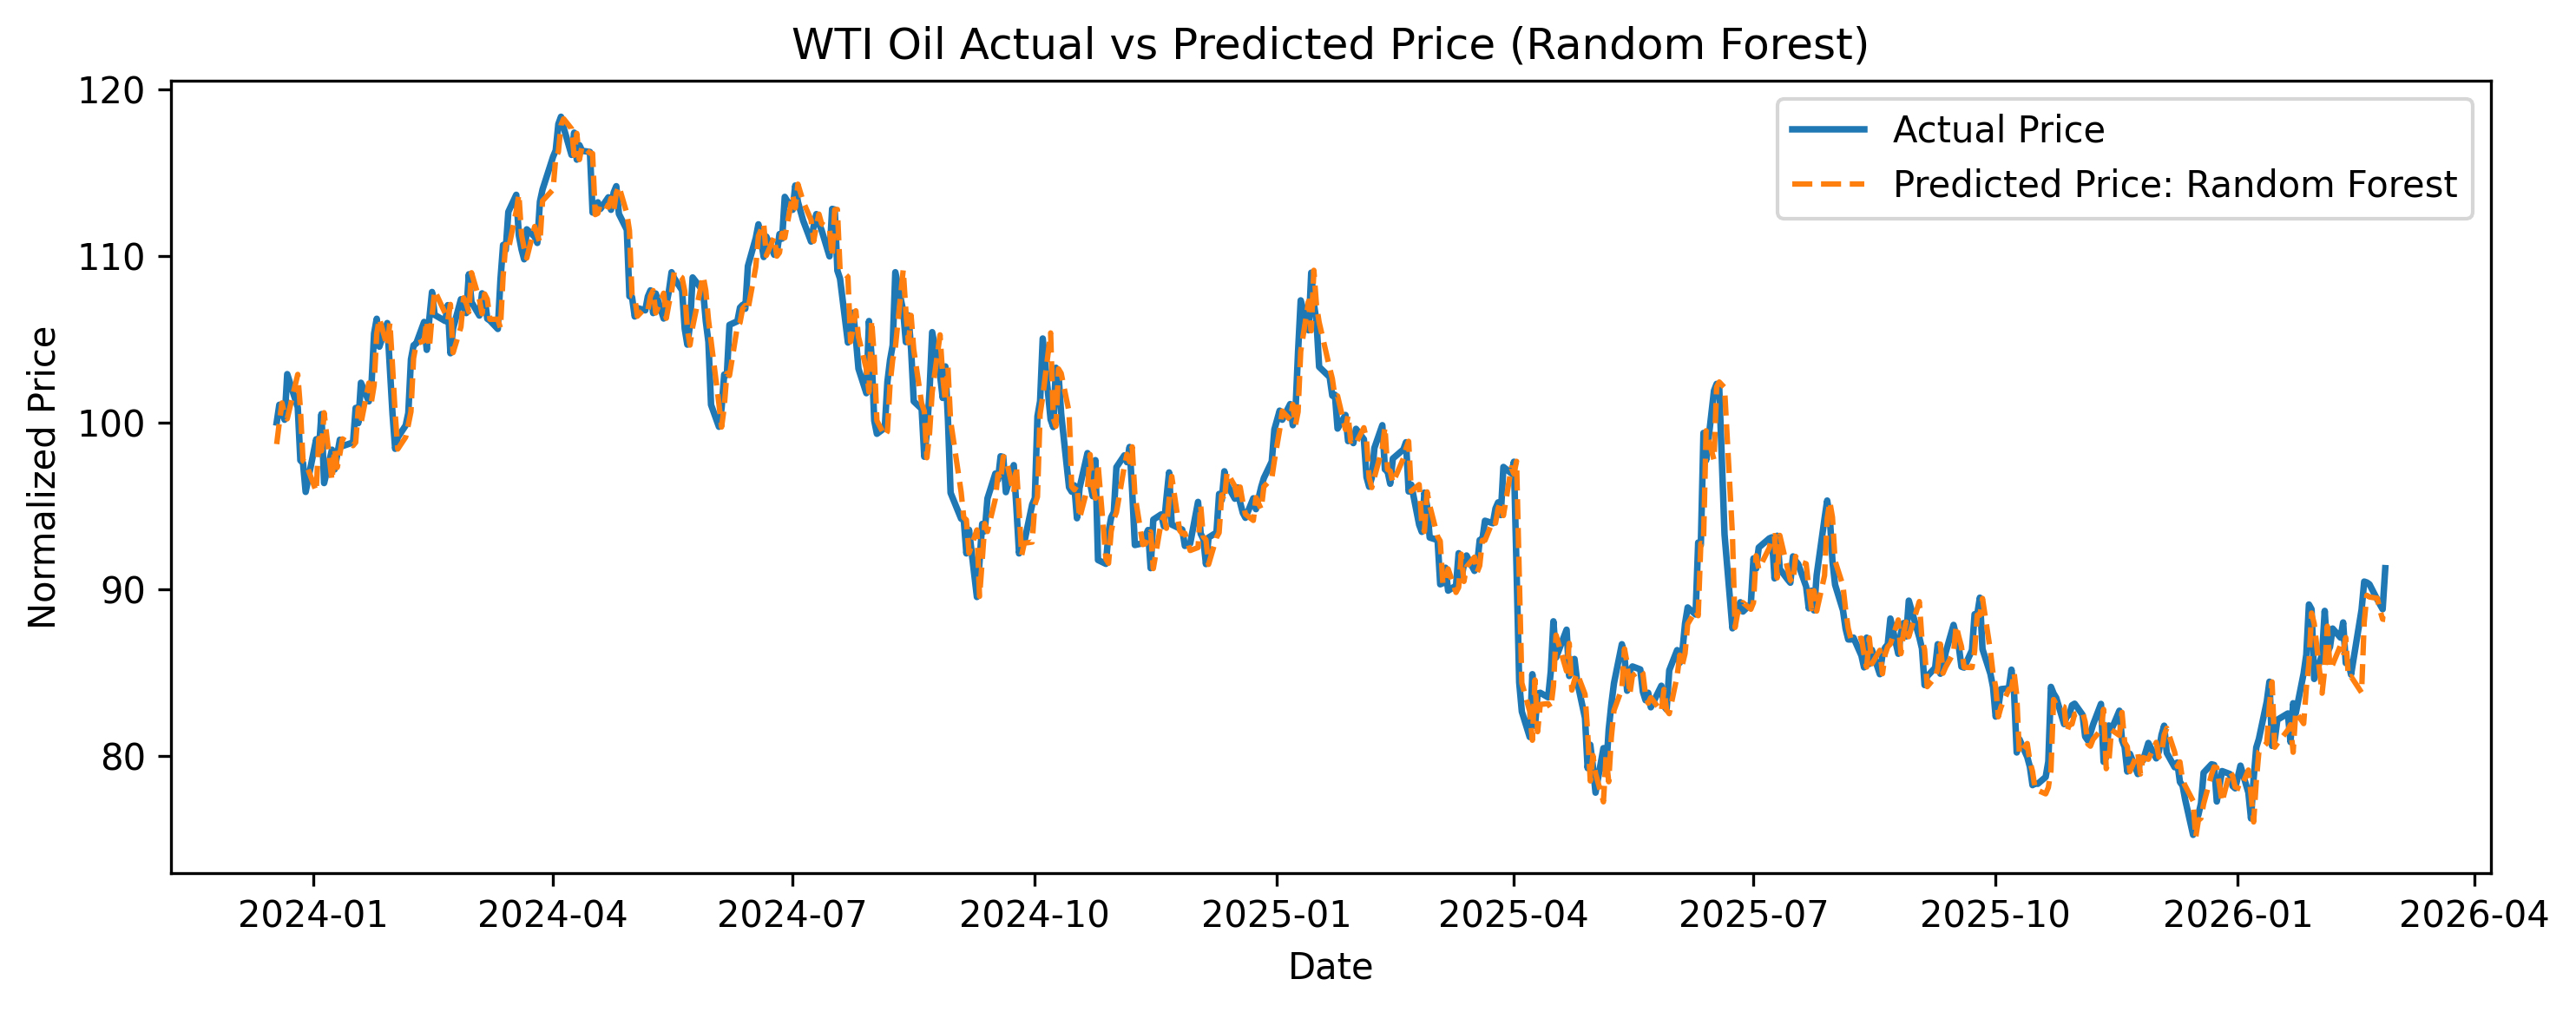
\includegraphics[width=\textwidth, trim=0 6 0 6, clip]{modeling_plot/WTI_Oil_Random_Forest_price_prediction.png}
        \caption{WTI Oil -- RF}
    \end{subfigure}
    \hspace{0.025\textwidth}
    \begin{subfigure}[t]{0.29\textwidth}
        \centering
        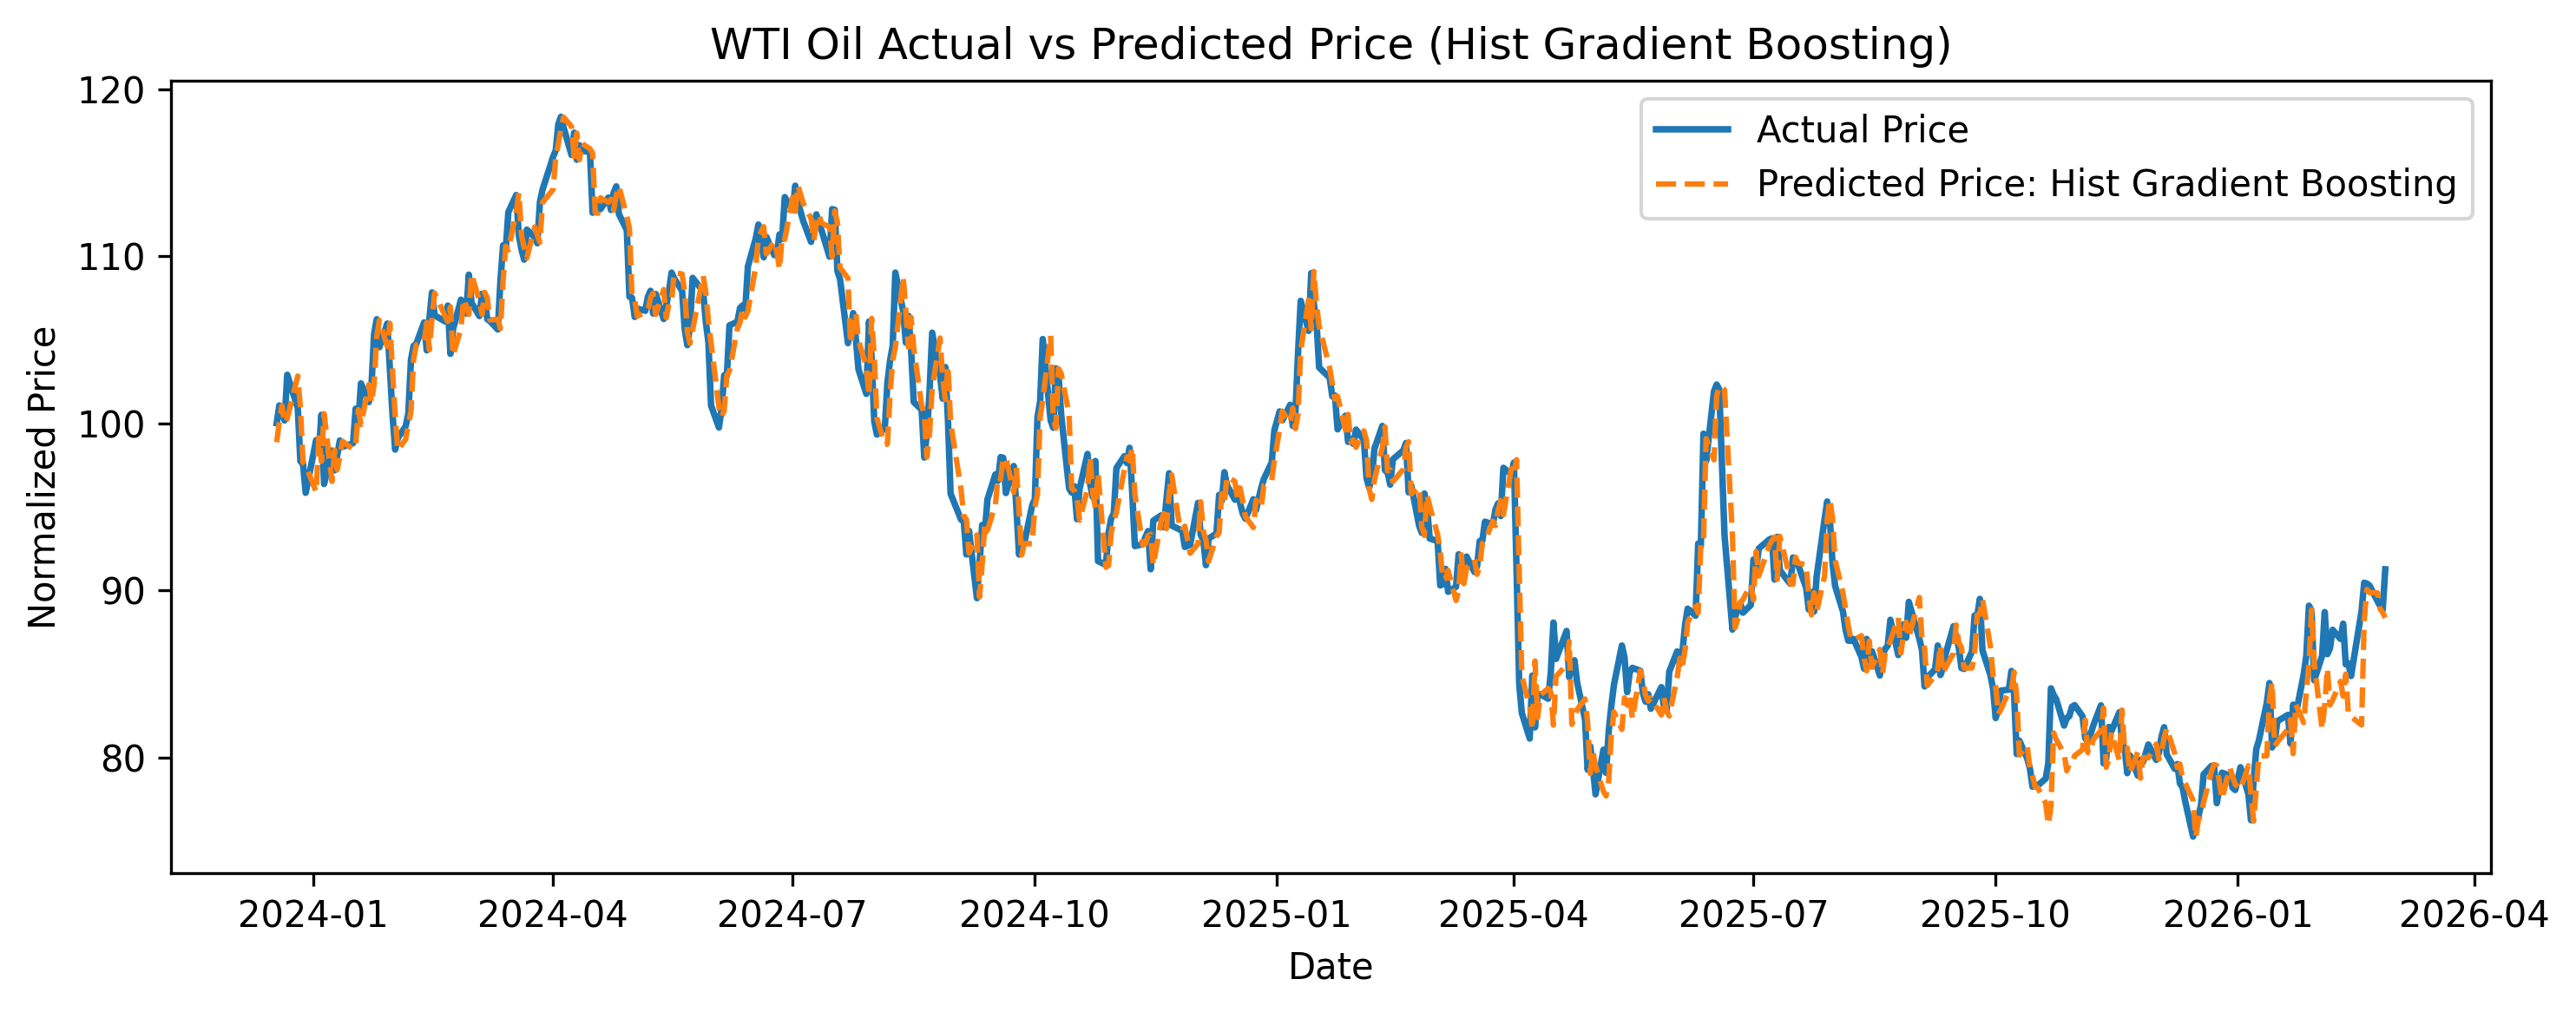
\includegraphics[width=\textwidth, trim=0 6 0 6, clip]{modeling_plot/WTI_Oil_Hist_Gradient_Boosting_price_prediction.png}
        \caption{WTI Oil -- HGB}
    \end{subfigure}

    \vspace{0.12cm}
    \caption{Actual vs Predicted Prices for USD Index and WTI Oil}
    \label{fig:price_predictions_macro}
\end{figure}

Figures \ref{fig:price_predictions_crypto}, \ref{fig:price_predictions_metals}, and \ref{fig:price_predictions_macro} show that the predicted price paths generally follow the broad
direction of the actual market movements. The prediction performance differs across assets.
Gold, Silver, and USD Index have smoother price paths, so the predicted curves are visually
closer to the actual series. Bitcoin, Ethereum, and WTI Oil show larger fluctuations, making
accurate prediction more difficult.

These figures are useful because they complement the numerical evaluation metrics.
While RMSE and MAE summarize average prediction errors, the price prediction plots show
whether each model can visually track turning points, local fluctuations, and overall market
trends. Therefore, they provide an intuitive way to assess how well the supervised models
reconstruct the observed price dynamics.

% ============================================================
% 6.8 Results and Model Comparison
% ============================================================

\subsection{Results and Model Comparison}

Table~\ref{tab:best_model_summary} summarizes the best-performing model for each asset, selected according to the lowest test RMSE. This table is the main summary table because it directly answers which model works best for each asset.

\begin{table}[htbp]
\centering
\caption{Best Supervised Model for Each Asset}
\label{tab:best_model_summary}
\resizebox{\textwidth}{!}{
\begin{tabular}{l l c c c c c}
\toprule
Asset & Best Model & MSE & RMSE & MAE & $R^2$ & Directional Accuracy \\
\midrule
Gold      & Random Forest           & 0.000173 & 0.013134 & 0.009076 & -0.011381 & 0.558182 \\
Silver    & Hist Gradient Boosting  & 0.000874 & 0.029571 & 0.018103 &  0.032746 & 0.476364 \\
WTI Oil   & Random Forest           & 0.000382 & 0.019551 & 0.015056 & -0.035923 & 0.492727 \\
USD Index & Random Forest           & 0.000017 & 0.004142 & 0.003098 & -0.001061 & 0.496364 \\
Bitcoin   & Random Forest           & 0.001005 & 0.031702 & 0.023146 & -0.011499 & 0.470909 \\
Ethereum  & Random Forest           & 0.001981 & 0.044510 & 0.032230 & -0.009862 & 0.467273 \\
\bottomrule
\end{tabular}
}
\end{table}

Overall, Random Forest achieved the best predictive performance for five of the six assets, while Hist Gradient Boosting performed best for Silver. This suggests that nonlinear tree-based models are generally more suitable than the linear Ridge Regression benchmark for the engineered financial feature set used in this project.

Among the six assets, USD Index had the smallest absolute prediction error, while Bitcoin and Ethereum had larger RMSE and MAE values. This is consistent with the exploratory analysis, where cryptocurrencies showed stronger volatility and more extreme return behavior.

Table \ref{tab:all_model_results} provides the full comparison of all three supervised models for each asset. This table is used to examine whether the selected best models in Table \ref{tab:best_model_summary} are consistently better than the alternative models.

\begin{table}[htbp]
\centering
\caption{Prediction Performance of All Supervised Models}
\label{tab:all_model_results}
\resizebox{\textwidth}{!}{
\begin{tabular}{l l c c c c c}
\toprule
Asset & Model & MSE & RMSE & MAE & $R^2$ & Directional Accuracy \\
\midrule
Bitcoin  & Random Forest          & 0.001005 & 0.031702 & 0.023146 & -0.011499 & 0.470909 \\
Bitcoin  & Ridge Regression       & 0.001048 & 0.032374 & 0.023723 & -0.054872 & 0.532727 \\
Bitcoin  & Hist Gradient Boosting & 0.001156 & 0.034004 & 0.025246 & -0.163705 & 0.465455 \\
\midrule
Ethereum & Random Forest          & 0.001981 & 0.044510 & 0.032230 & -0.009862 & 0.467273 \\
Ethereum & Hist Gradient Boosting & 0.002005 & 0.044780 & 0.032587 & -0.022153 & 0.483636 \\
Ethereum & Ridge Regression       & 0.002089 & 0.045704 & 0.033004 & -0.064739 & 0.510909 \\
\midrule
Gold     & Random Forest          & 0.000173 & 0.013134 & 0.009076 & -0.011381 & 0.558182 \\
Gold     & Hist Gradient Boosting & 0.000176 & 0.013252 & 0.009254 & -0.029533 & 0.514545 \\
Gold     & Ridge Regression       & 0.000178 & 0.013339 & 0.009362 & -0.043203 & 0.465455 \\
\midrule
Silver   & Hist Gradient Boosting & 0.000874 & 0.029571 & 0.018103 &  0.032746 & 0.476364 \\
Silver   & Random Forest          & 0.000907 & 0.030114 & 0.018179 & -0.003125 & 0.478182 \\
Silver   & Ridge Regression       & 0.000923 & 0.030375 & 0.018690 & -0.020576 & 0.478182 \\
\midrule
USD Index& Random Forest          & 0.000017 & 0.004142 & 0.003098 & -0.001061 & 0.496364 \\
USD Index& Hist Gradient Boosting & 0.000017 & 0.004178 & 0.003136 & -0.018698 & 0.509091 \\
USD Index& Ridge Regression       & 0.000017 & 0.004179 & 0.003125 & -0.019161 & 0.512727 \\
\midrule
WTI Oil  & Random Forest          & 0.000382 & 0.019551 & 0.015056 & -0.035923 & 0.492727 \\
WTI Oil  & Hist Gradient Boosting & 0.000454 & 0.021302 & 0.016182 & -0.229759 & 0.500000 \\
WTI Oil  & Ridge Regression       & 0.000535 & 0.023139 & 0.017450 & -0.451073 & 0.507273 \\
\bottomrule
\end{tabular}
}
\end{table}

The full model comparison shows that the performance differences among the three models are sometimes small, especially for assets such as USD Index and Gold. However, Random Forest is still the most consistent model across assets, while Hist Gradient Boosting is competitive and achieves the lowest RMSE for Silver. Ridge Regression generally performs slightly worse, suggesting that a purely linear model may not fully capture the nonlinear relationships in the engineered financial features.

The $R^2$ values are generally low or negative. This does not necessarily mean that the models are useless, because short-horizon financial return prediction is highly noisy and difficult. In this setting, even a model with low $R^2$ can still be useful if it reduces RMSE or MAE relative to other models and produces reasonable price-path behavior. Therefore, the model results should be interpreted together with RMSE, MAE, directional accuracy, and the price prediction plots.

\subsection{Summary}

In summary, three supervised learning models were compared for forecasting the next-day log returns of six financial assets: Gold, Silver, WTI Oil, USD Index, Bitcoin, and Ethereum. The models included one linear benchmark model, Ridge Regression, and two nonlinear tree-based ensemble models, Random Forest and Hist Gradient Boosting.

The results show that the nonlinear ensemble models generally performed better than the linear Ridge Regression baseline. Random Forest achieved the best RMSE for five of the six assets, including Gold, WTI Oil, USD Index, Bitcoin, and Ethereum, while Hist Gradient Boosting performed best for Silver. This suggests that the relationship between engineered market features and future returns is not purely linear, and nonlinear models are better able to capture interactions among lagged returns, volatility measures, momentum variables, rolling correlations, drawdown features, and extreme-return indicators.

In addition to the numerical metrics, the return prediction plots provide a more direct view of the forecasting task. Since the models are trained to predict next-day log returns rather than prices directly, these plots show whether the models can capture the direction, magnitude, and volatility of daily return movements. The return plots also explain why price prediction curves may look close even when return prediction remains difficult, because small daily return errors can accumulate differently when converted into price paths.

The prediction difficulty also differed across assets. USD Index had the smallest prediction errors, which is consistent with its relatively stable return behavior observed in the exploratory analysis. In contrast, Bitcoin and Ethereum had larger RMSE and MAE values, reflecting their higher volatility and more extreme price movements. This confirms that cryptocurrencies are more difficult to forecast than relatively stable traditional assets.

Overall, the supervised learning results support the usefulness of the extended feature engineering process. The engineered features provided meaningful information for the models, and the tree-based methods were able to use these features more effectively than the linear benchmark. Therefore, Random Forest can be considered the strongest overall supervised model in this project, while Hist Gradient Boosting remains a competitive alternative for some assets.

% ============================================================
% 7. Numerical Method Validation
% ============================================================

\section{Numerical Method Validation}

After obtaining predicted next-day returns from the three supervised learning models, we further applied numerical validation methods to reconstruct predicted price paths and evaluate whether the forecasted returns could produce realistic price trajectories. This step serves as an additional robustness check for the supervised learning results.

The purpose of numerical validation is not to replace the supervised learning models, but to assess how different numerical updating schemes affect the conversion from predicted returns to predicted prices. In this project, we compared three numerical methods: the Euler method, the Trapezoidal method, and an RK4-like method.

\subsection{Validation Framework}

For each asset and each supervised learning model, the predicted next-day log return $\hat{r}_{t+1}$ was converted into a predicted next-day price using numerical updating rules. Let $P_t$ denote the actual price at time $t$, and let $\hat{P}_{t+1}$ denote the predicted price for time $t+1$.

\paragraph{Euler Method}
The Euler method uses the predicted next-day return directly:
\[
\hat{P}_{t+1}^{(E)} = P_t \exp(\hat{r}_{t+1}).
\]

\paragraph{Trapezoidal Method}
The Trapezoidal method averages the return at the current step and the return implied by the next prediction:
\[
\hat{P}_{t+1}^{(T)} = P_t \exp\left(\frac{\hat{r}_t + \hat{r}_{t+1}}{2}\right).
\]

\paragraph{RK4-like Method}
To further smooth the predicted path, we also implemented an RK4-like updating rule based on weighted intermediate return estimates:
\[
\hat{P}_{t+1}^{(RK4)} = P_t \exp\left(\frac{k_1 + 2k_2 + 2k_3 + k_4}{6}\right),
\]
where $k_1, k_2, k_3,$ and $k_4$ are intermediate return approximations constructed from the predicted returns. Although this is not a continuous-time differential equation setting, the RK4-like rule provides a more flexible benchmark for validation.

For each asset-model combination, the numerical method that achieved the smallest prediction error was recorded as the best validation method.

\subsection{Evaluation Metrics}

To evaluate the effectiveness of the numerical validation methods, we compared the reconstructed price paths with the actual observed prices using the following three metrics:

\paragraph{Root Mean Squared Error (RMSE)}
\[
RMSE = \sqrt{\frac{1}{n}\sum_{i=1}^{n}(P_{i,\text{actual}} - P_{i,\text{predicted}})^2}.
\]

\paragraph{Mean Absolute Error (MAE)}
\[
MAE = \frac{1}{n}\sum_{i=1}^{n}\left|P_{i,\text{actual}} - P_{i,\text{predicted}}\right|.
\]

\paragraph{Mean Absolute Percentage Error (MAPE)}
\[
MAPE = \frac{100}{n}\sum_{i=1}^{n}\left|\frac{P_{i,\text{actual}} - P_{i,\text{predicted}}}{P_{i,\text{actual}}}\right|.
\]

Among these metrics, RMSE was used as the primary criterion for selecting the best numerical validation method.

\subsection{Summary of Numerical Validation Results}

The numerical validation results show that the Euler method most frequently achieved the lowest prediction error across asset-model combinations. Among the 18 asset-model combinations, Euler was selected as the best numerical method in 12 cases, Trapezoidal in 5 cases, and RK4-like in 1 case. This indicates that a simple one-step price updating rule is generally sufficient for this project.

Across the six assets, Random Forest combined with Euler updating produced the best overall performance for Bitcoin, Ethereum, Gold, USD Index, and WTI Oil. For Silver, Hist Gradient Boosting combined with Euler updating achieved the lowest RMSE. These findings are consistent with the supervised learning results, where Random Forest was the strongest overall model and Hist Gradient Boosting performed competitively for Silver.

The differences among Euler, Trapezoidal, and RK4-like methods are relatively small in most cases. Therefore, the numerical validation step mainly confirms the robustness of the machine learning prediction paths rather than replacing the supervised learning models. Since the task is based on discrete daily return forecasting rather than continuous-time differential equation solving, the simpler Euler method often performs as well as or better than the more complicated validation methods.

\begin{table}[H]
\centering
\caption{Best Numerical Validation Combination by Asset}
\label{tab:best_numerical_validation}
\begin{tabular}{llllrrr}
\toprule
Asset & Best Model & Best Numerical Method & RMSE & MAE & MAPE (\%) \\
\midrule
Bitcoin   & Random Forest          & Euler & 2473.89 & 1842.42 & 2.31 \\
Ethereum  & Random Forest          & Euler & 134.33  & 96.74   & 3.23 \\
Gold      & Random Forest          & Euler & 50.69   & 29.81   & 0.91 \\
Silver    & Hist Gradient Boosting & Euler & 2.15    & 0.87    & 1.82 \\
USD Index & Random Forest          & Euler & 0.42    & 0.32    & 0.31 \\
WTI Oil   & Random Forest          & Euler & 1.35    & 1.04    & 1.51 \\
\bottomrule
\end{tabular}
\end{table}

\begin{table}[H]
\centering
\caption{Frequency of Best Numerical Validation Method}
\label{tab:numerical_method_frequency}
\begin{tabular}{lc}
\toprule
Numerical Method & Number of Best Cases \\
\midrule
Euler       & 12 \\
Trapezoidal & 5  \\
RK4-like    & 1  \\
\bottomrule
\end{tabular}
\end{table}

\subsection{Numerical Validation Plots}

Figures~\ref{fig:numerical_validation_crypto}, \ref{fig:numerical_validation_metals}, and \ref{fig:numerical_validation_macro} present the actual and numerically validated predicted price paths for all six assets under the three supervised learning models. In each row, the same asset is shown under Ridge Regression, Random Forest, and Hist Gradient Boosting, respectively. Overall, the predicted price trajectories follow the actual price movements closely, especially for Gold, Silver, USD Index, and WTI Oil. For Bitcoin and Ethereum, the models still capture the broad trend reasonably well, although the deviations are larger due to the higher volatility of cryptocurrency markets.

% ------------------------------------------------------------
% Figure: Bitcoin and Ethereum
% ------------------------------------------------------------

\begin{figure}[H]
    \centering
    \captionsetup[subfigure]{skip=4pt}
    
    % ---------------- Bitcoin ----------------
    \begin{subfigure}[t]{0.31\textwidth}
        \centering
        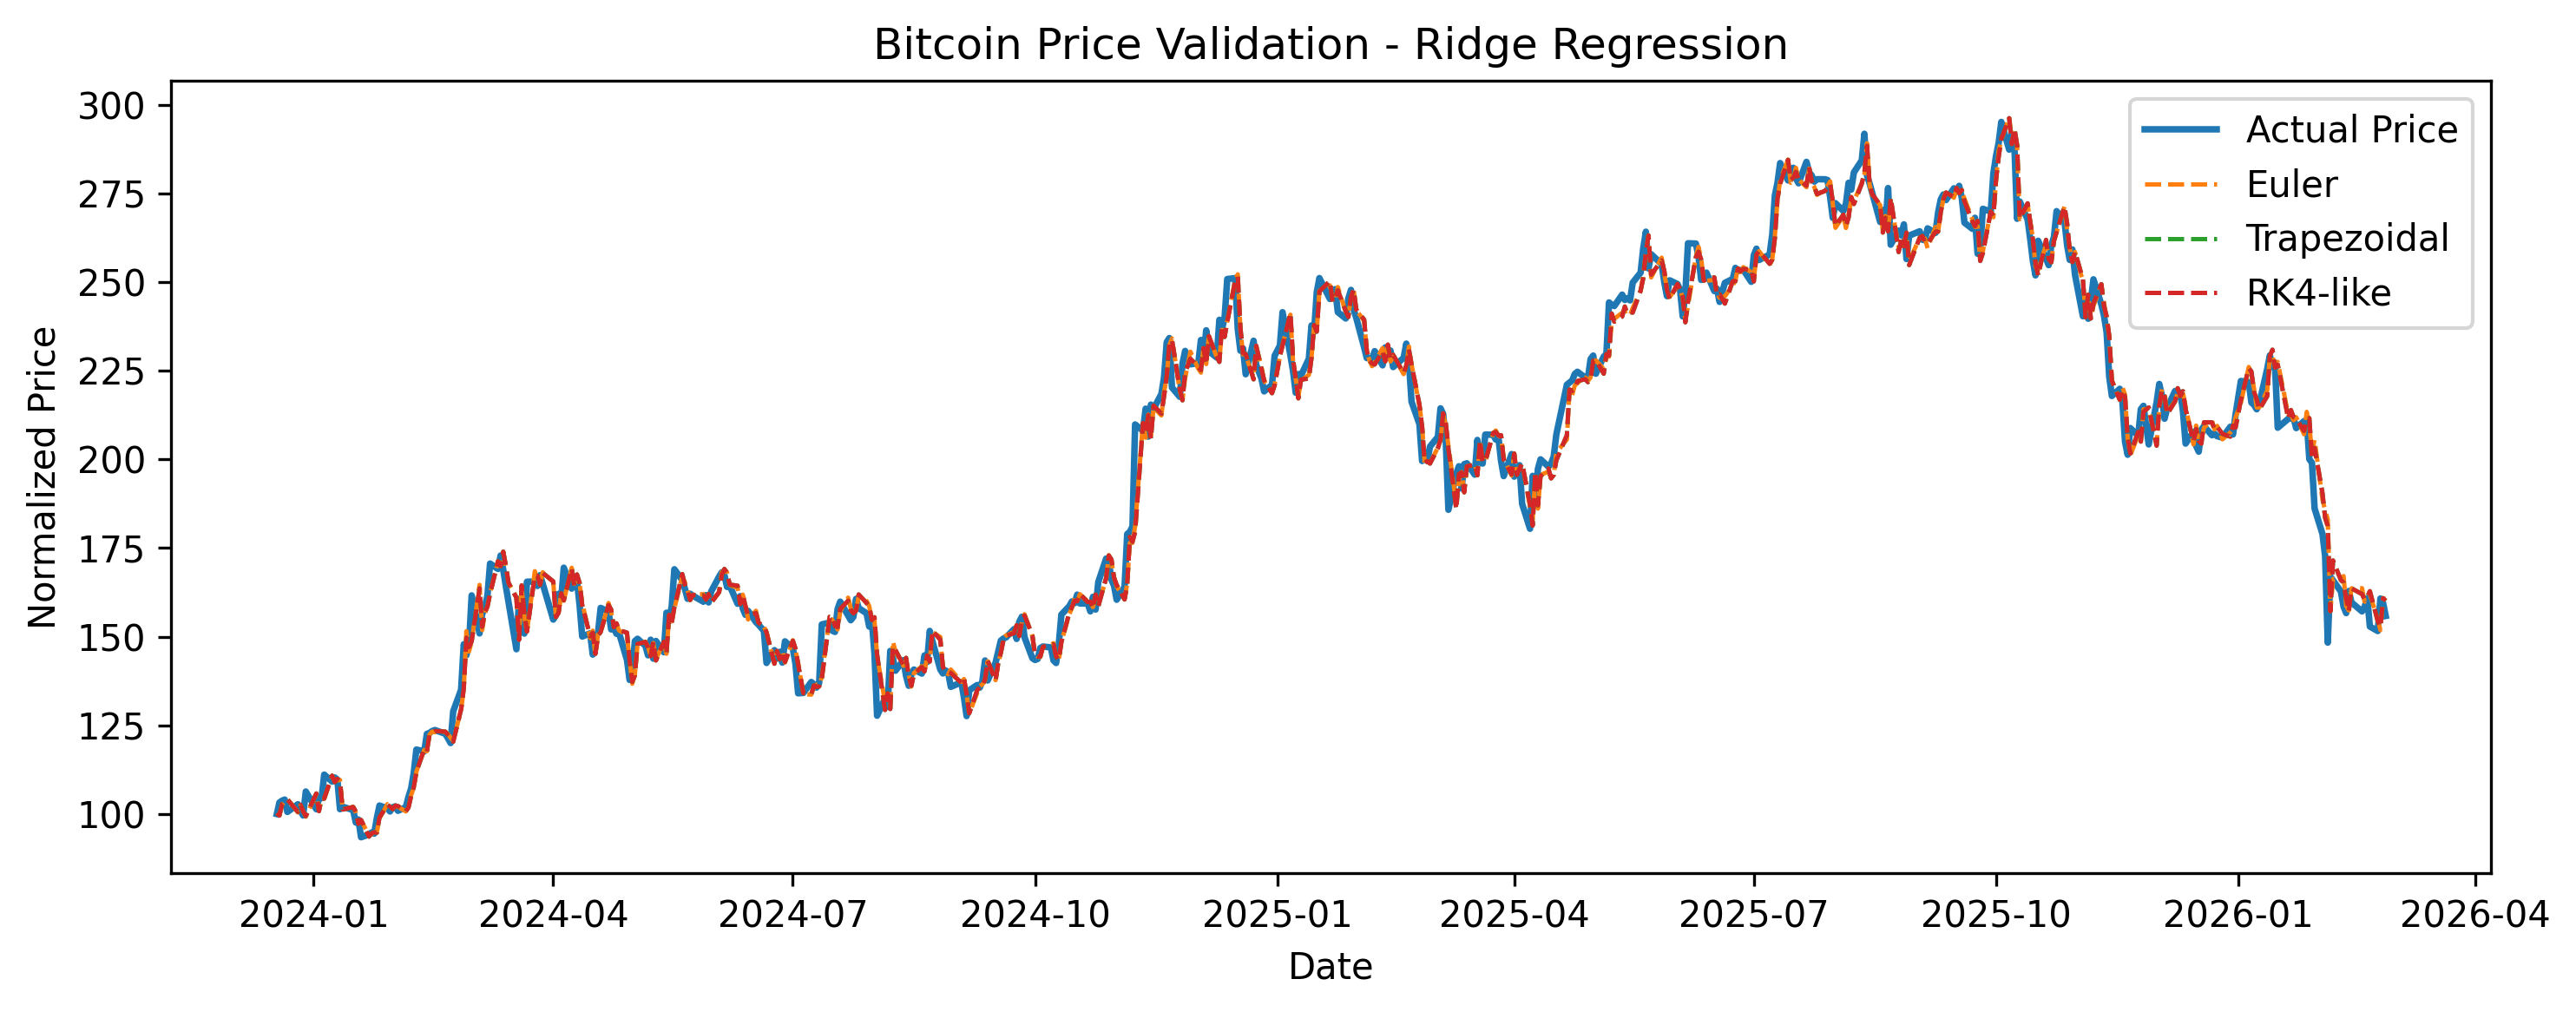
\includegraphics[width=\textwidth]{numerical_validation_plot/Bitcoin_Ridge_Regression_price_validation.png}
        \caption{Bitcoin -- Ridge}
    \end{subfigure}
    \hfill
    \begin{subfigure}[t]{0.31\textwidth}
        \centering
        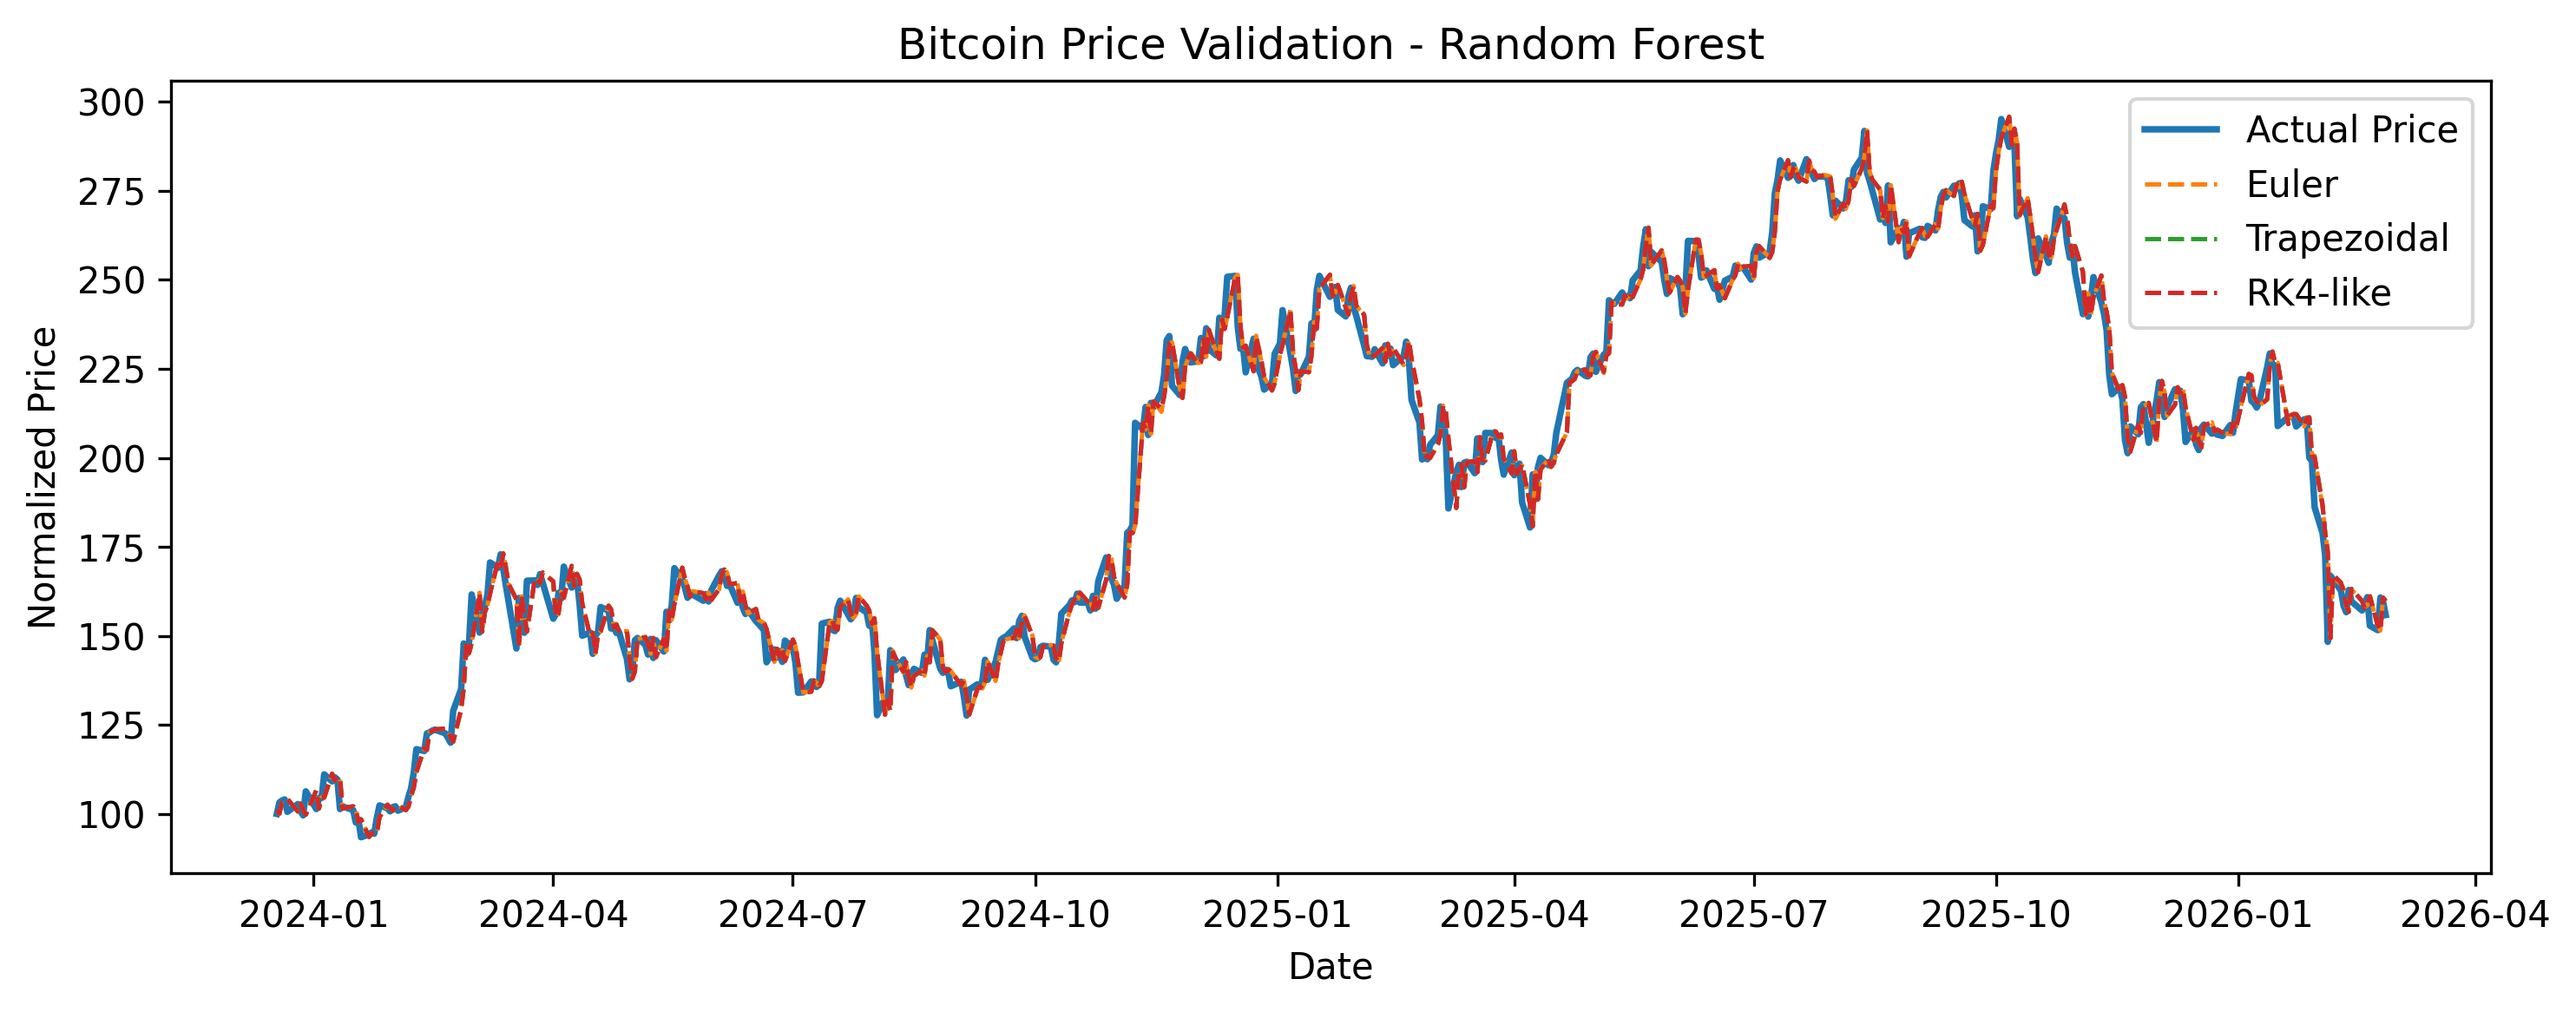
\includegraphics[width=\textwidth]{numerical_validation_plot/Bitcoin_Random_Forest_price_validation.png}
        \caption{Bitcoin -- RF}
    \end{subfigure}
    \hfill
    \begin{subfigure}[t]{0.31\textwidth}
        \centering
        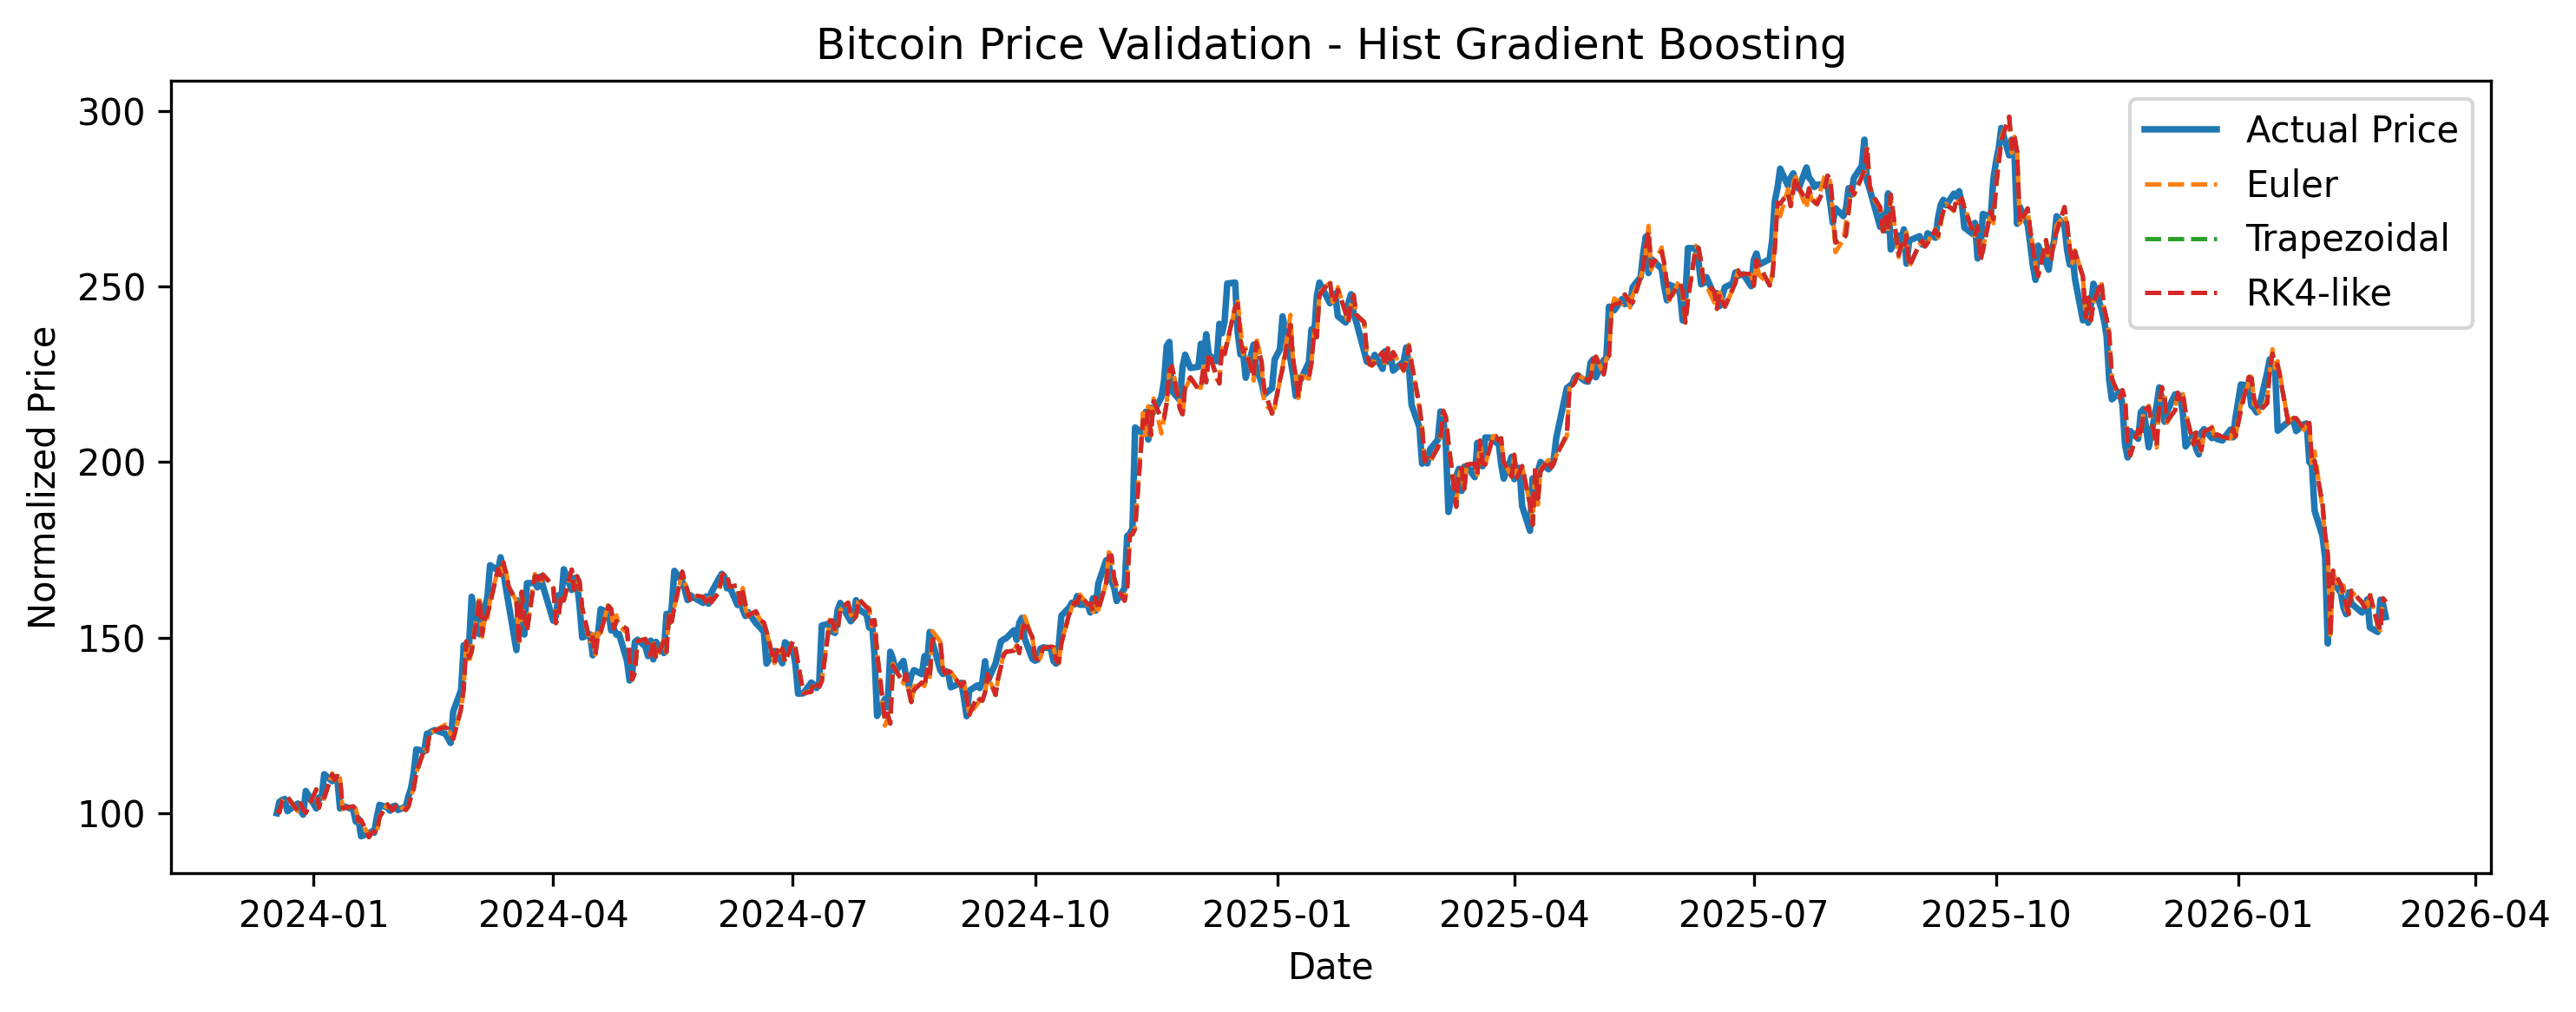
\includegraphics[width=\textwidth]{numerical_validation_plot/Bitcoin_Hist_Gradient_Boosting_price_validation.png}
        \caption{Bitcoin -- HGB}
    \end{subfigure}

    \vspace{0.15cm}

    % ---------------- Ethereum ----------------
    \begin{subfigure}[t]{0.31\textwidth}
        \centering
        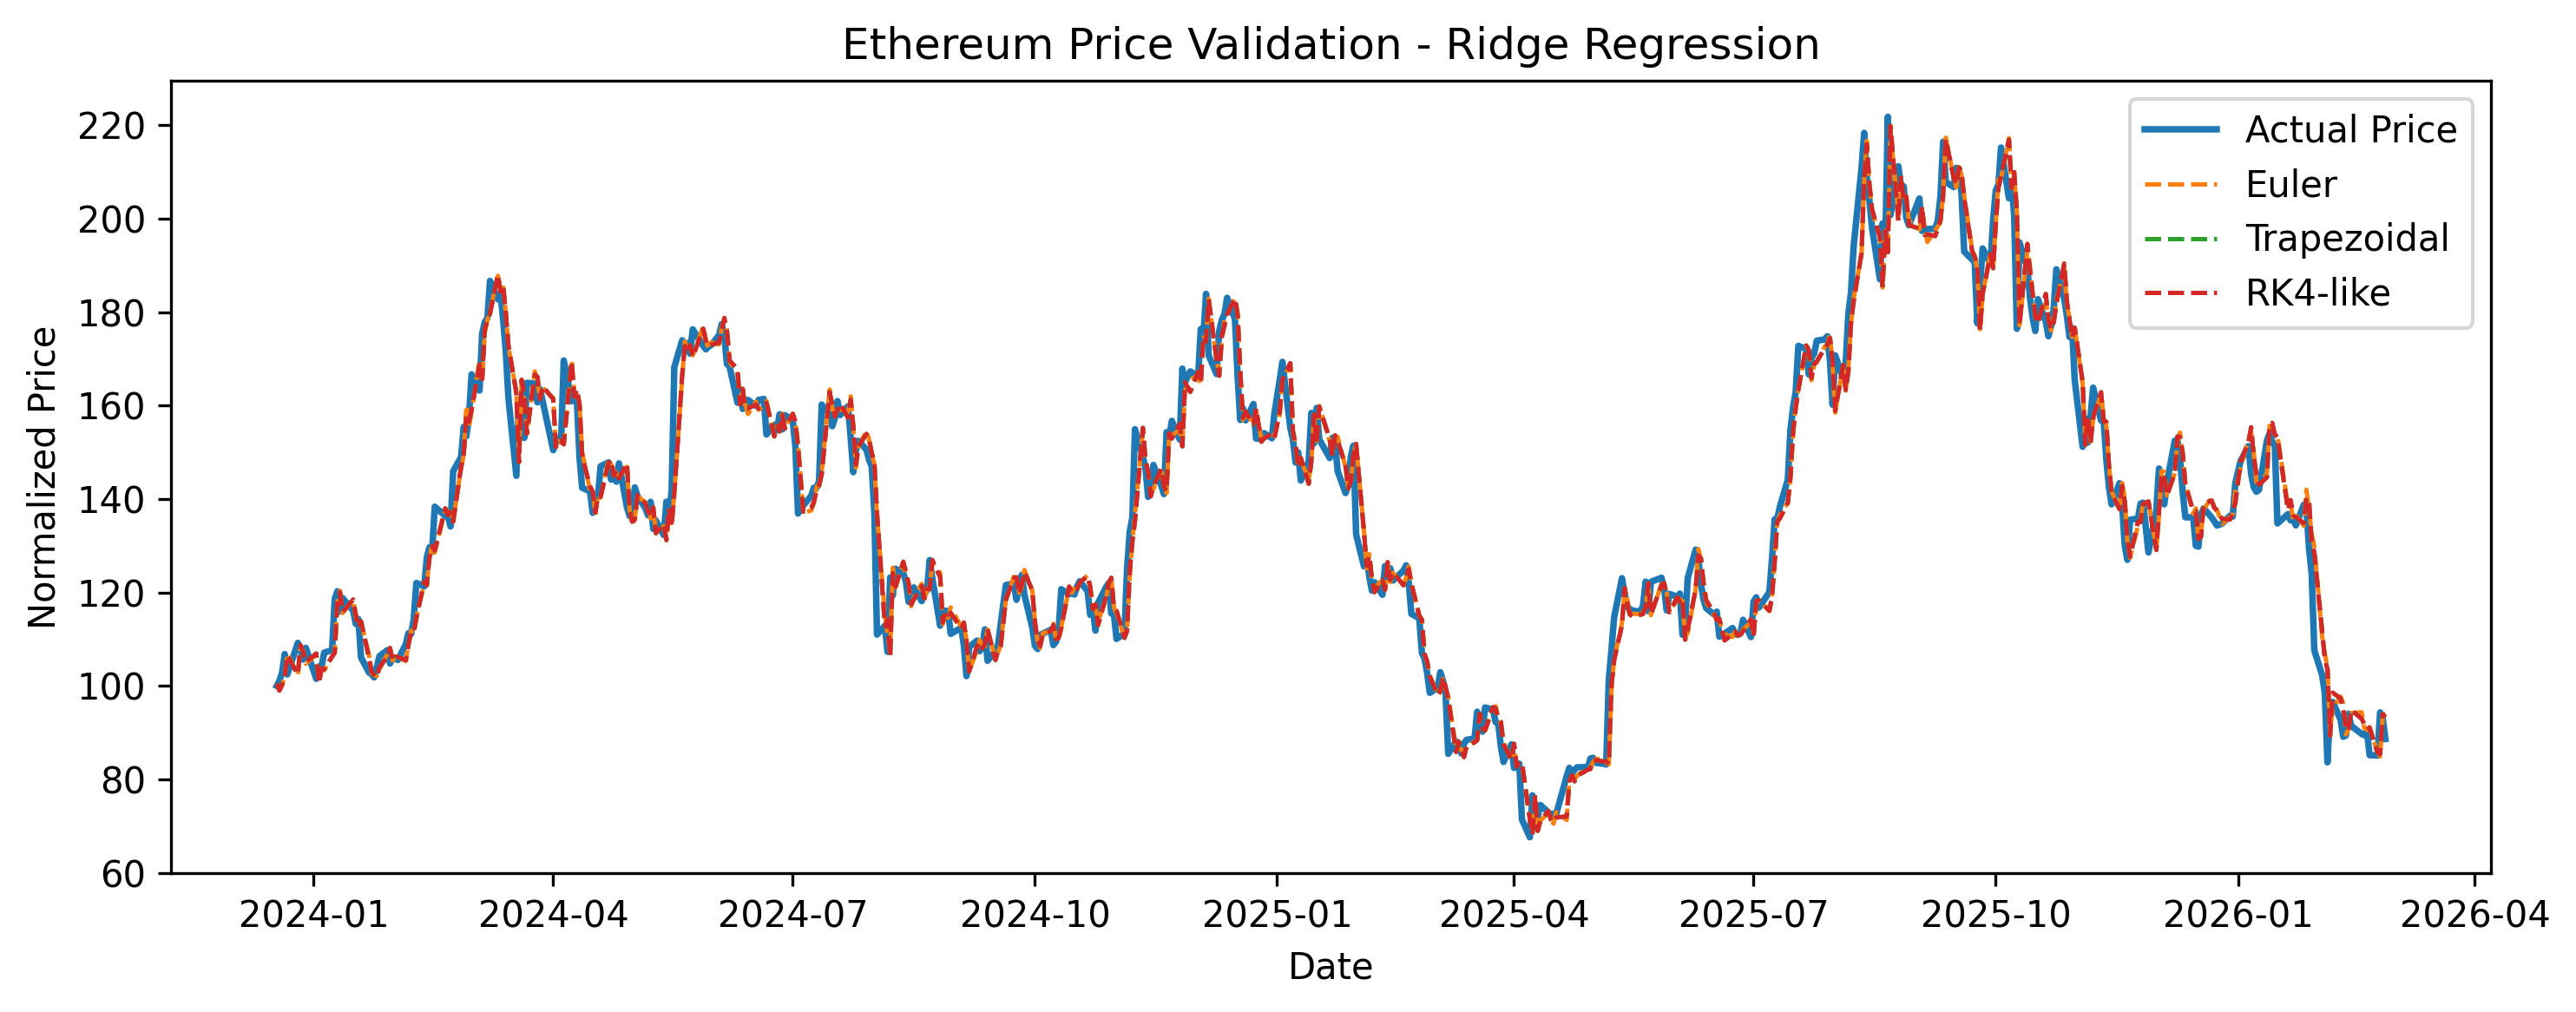
\includegraphics[width=\textwidth]{numerical_validation_plot/Ethereum_Ridge_Regression_price_validation.png}
        \caption{Ethereum -- Ridge}
    \end{subfigure}
    \hfill
    \begin{subfigure}[t]{0.31\textwidth}
        \centering
        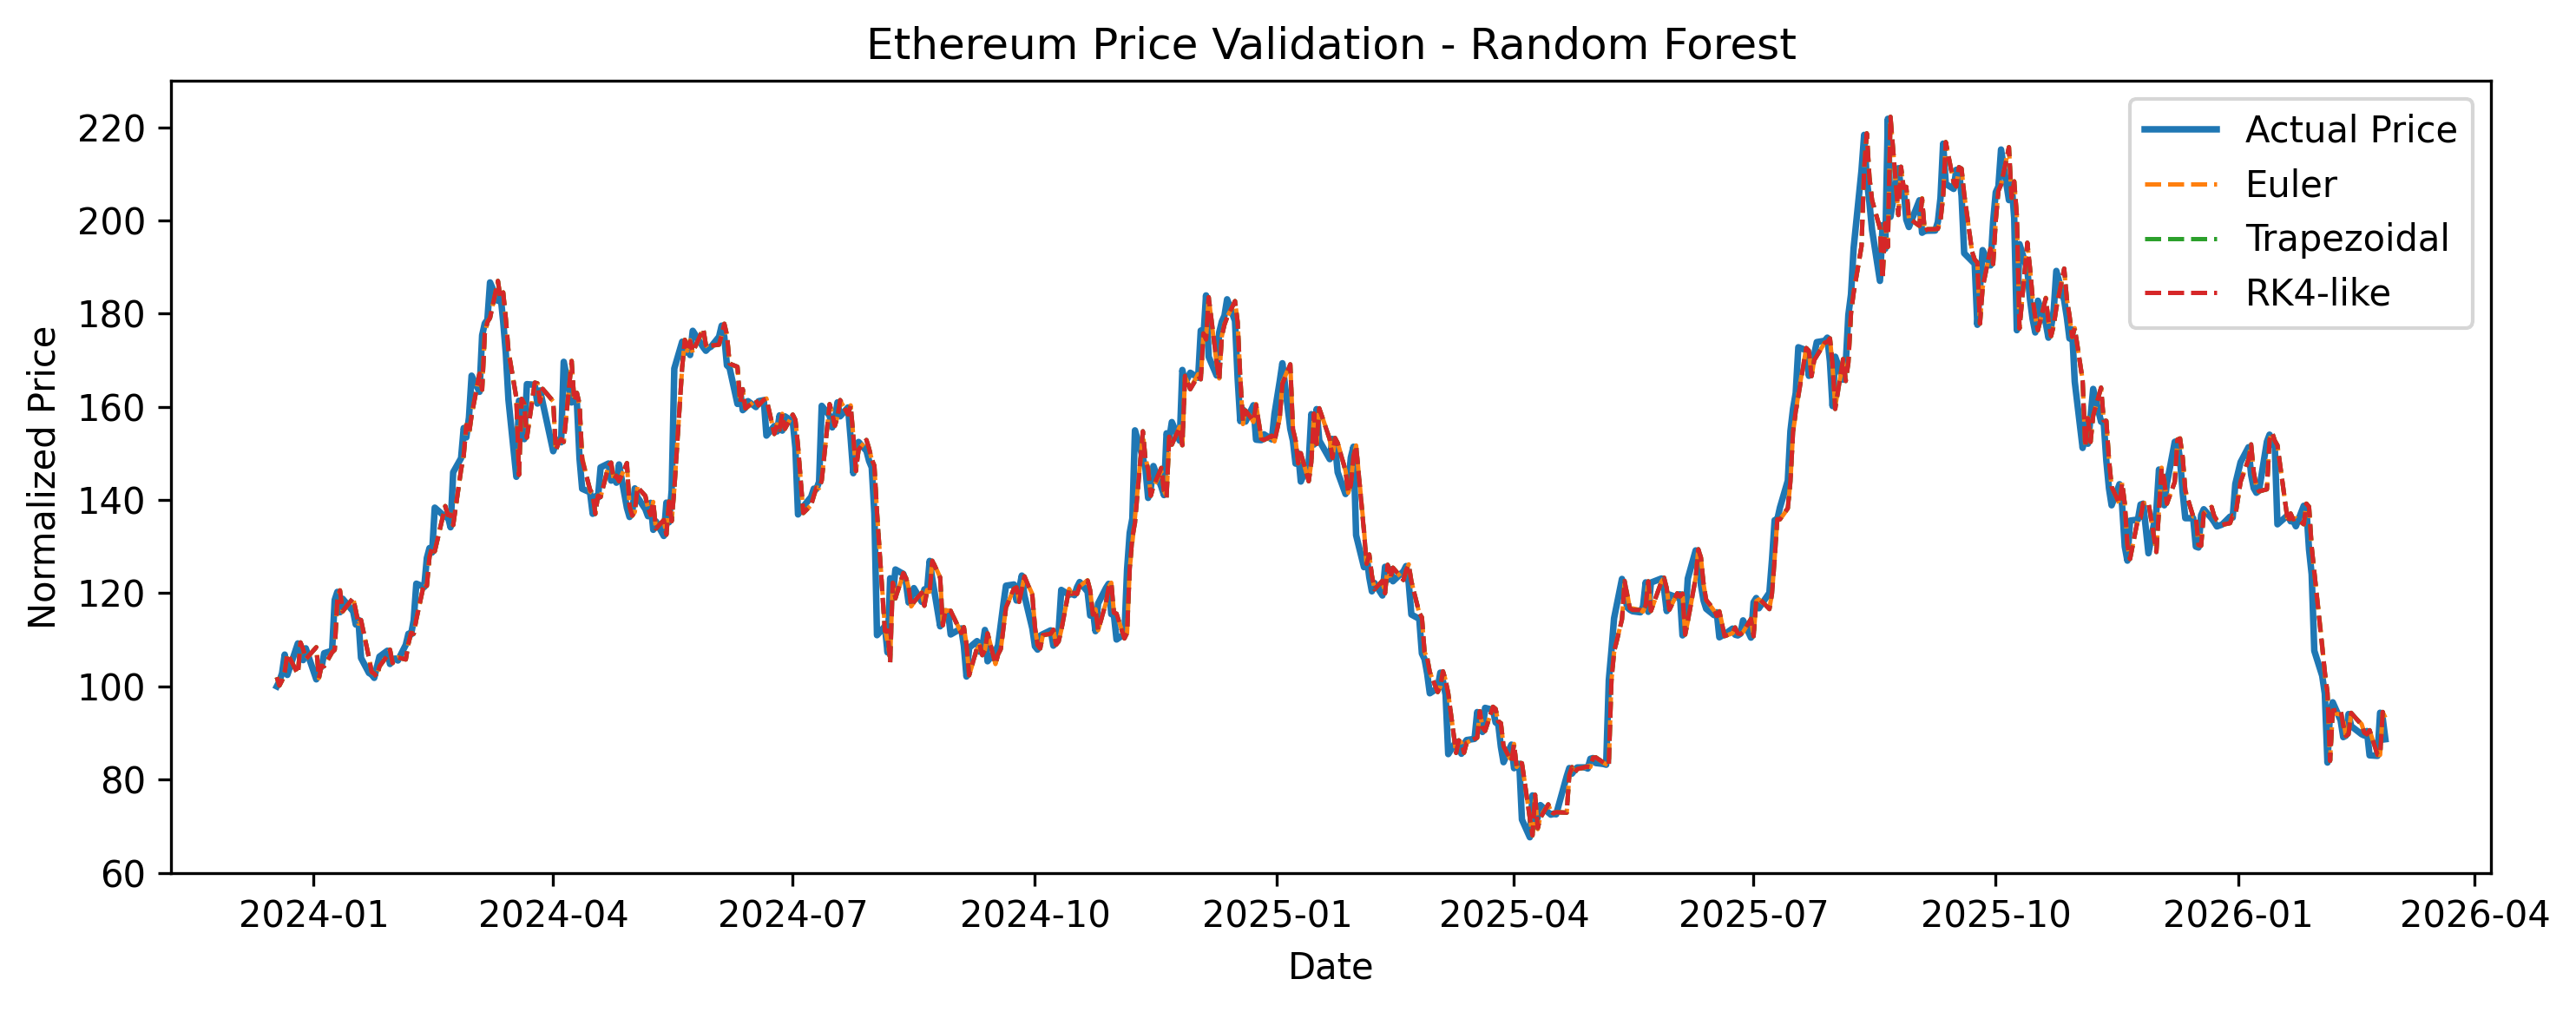
\includegraphics[width=\textwidth]{numerical_validation_plot/Ethereum_Random_Forest_price_validation.png}
        \caption{Ethereum -- RF}
    \end{subfigure}
    \hfill
    \begin{subfigure}[t]{0.31\textwidth}
        \centering
        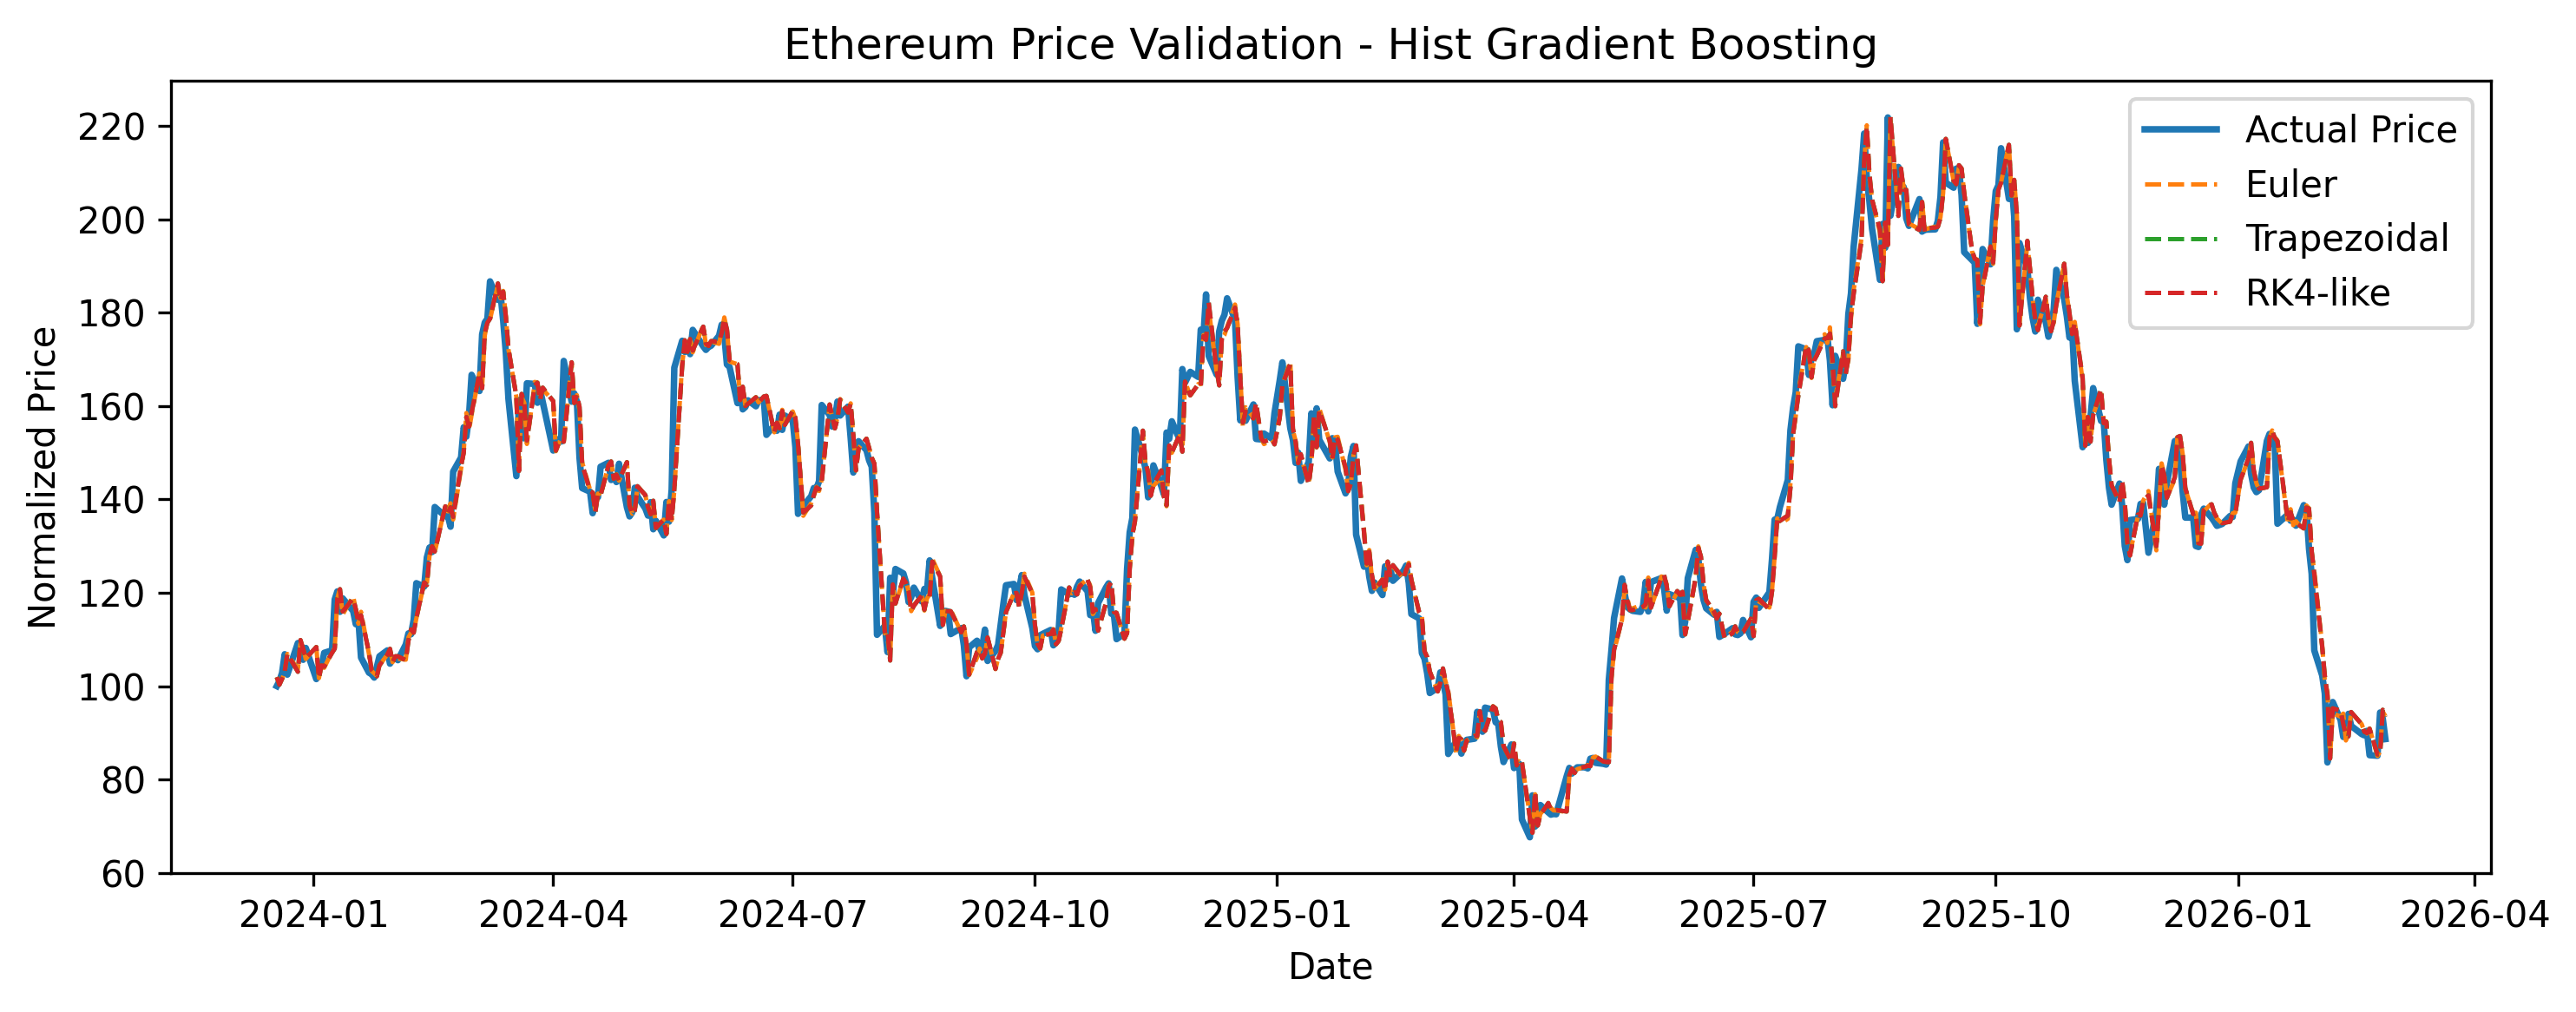
\includegraphics[width=\textwidth]{numerical_validation_plot/Ethereum_Hist_Gradient_Boosting_price_validation.png}
        \caption{Ethereum -- HGB}
    \end{subfigure}

    \caption{Actual vs Numerically Validated Predicted Prices for Bitcoin and Ethereum}
    \label{fig:numerical_validation_crypto}
\end{figure}

% ------------------------------------------------------------
% Figure: Gold and Silver
% ------------------------------------------------------------

\begin{figure}[H]
    \centering
    \captionsetup[subfigure]{skip=4pt}
    
    % ---------------- Gold ----------------
    \begin{subfigure}[t]{0.31\textwidth}
        \centering
        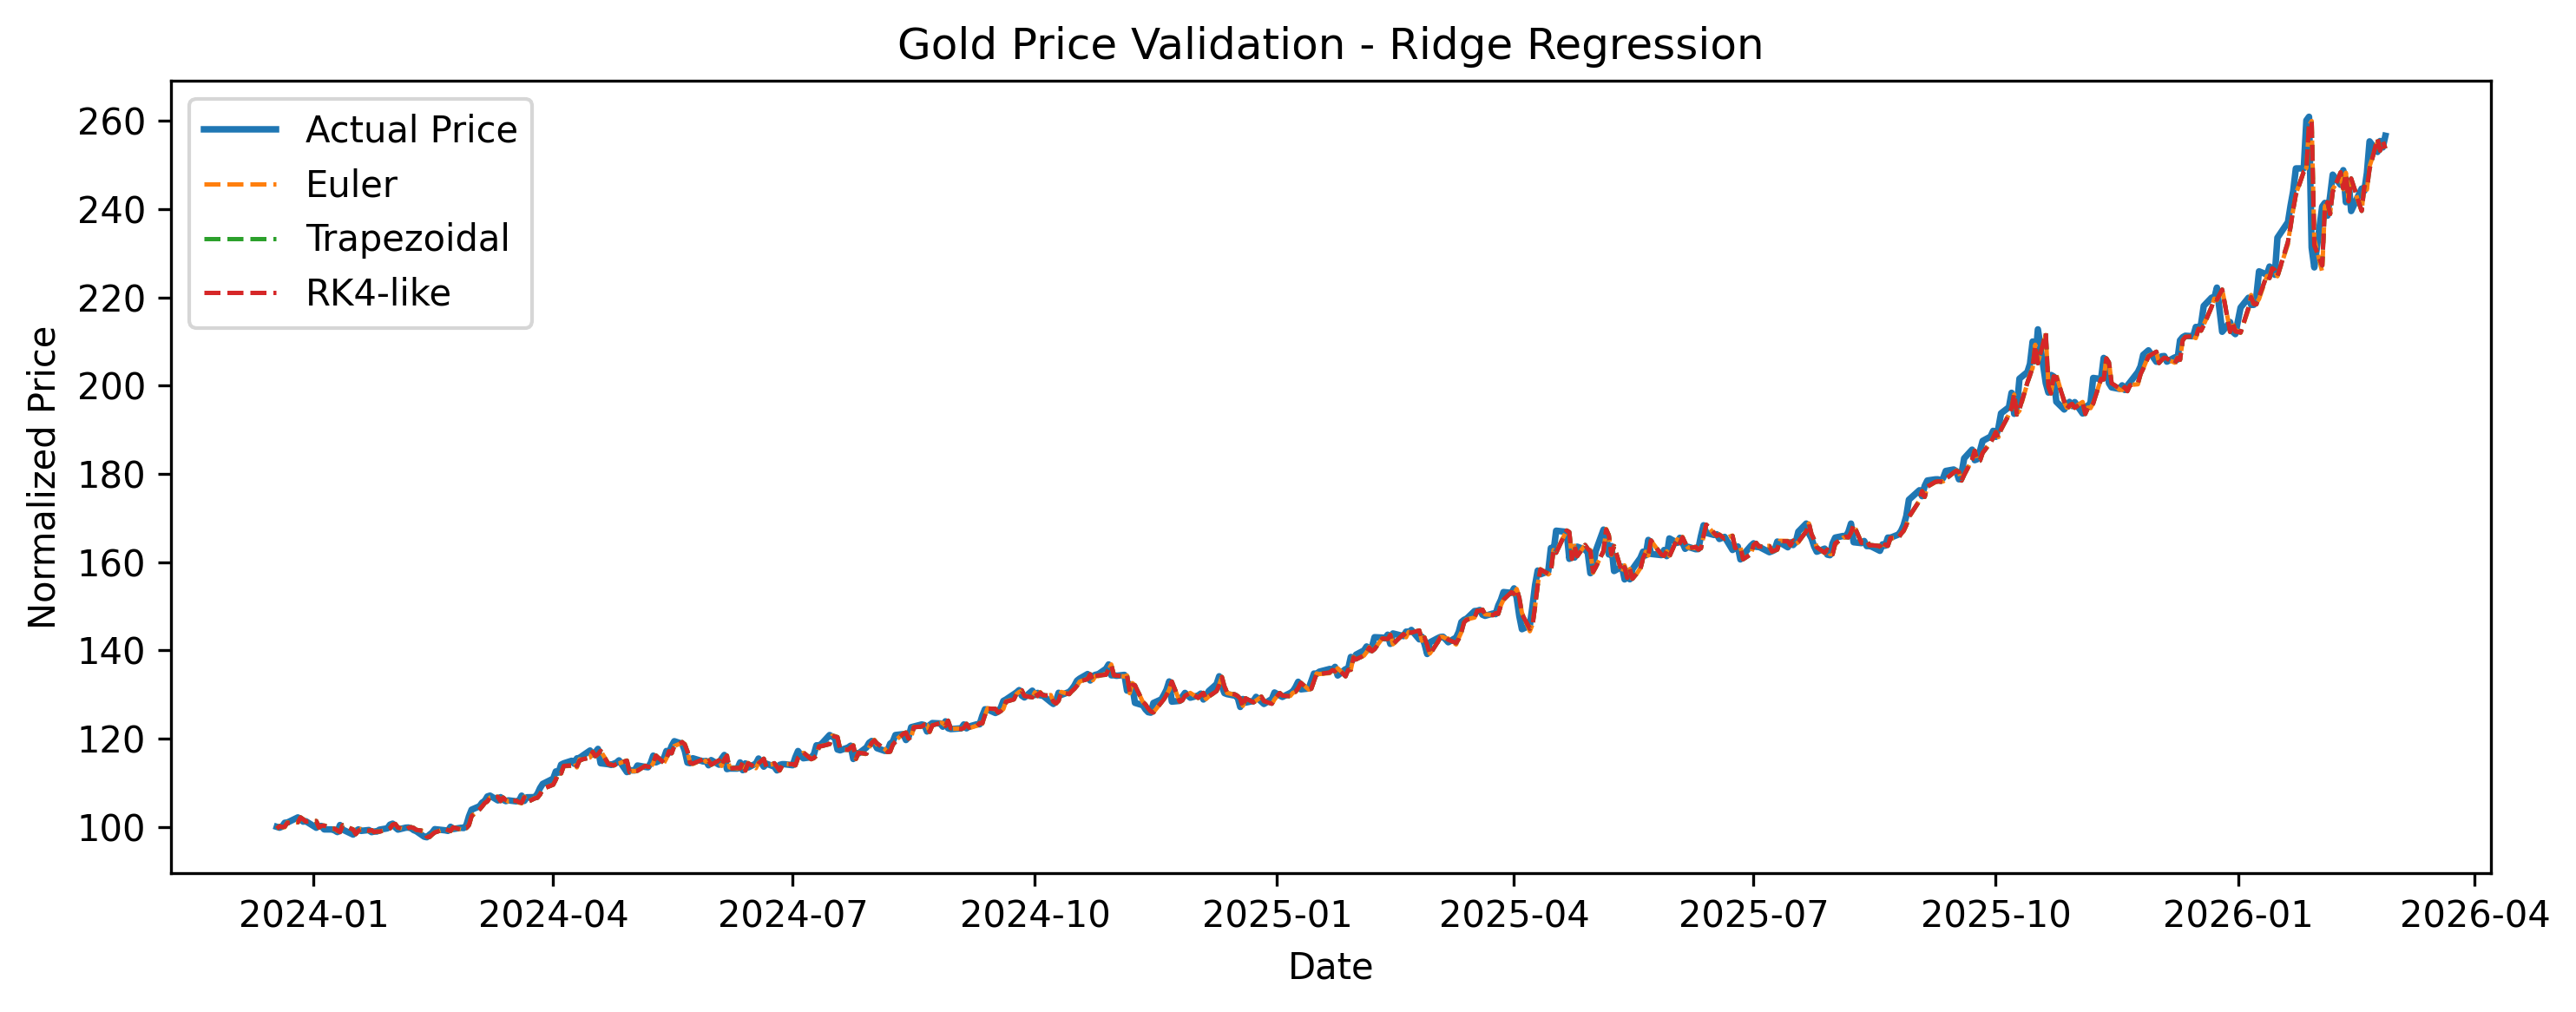
\includegraphics[width=\textwidth]{numerical_validation_plot/Gold_Ridge_Regression_price_validation.png}
        \caption{Gold -- Ridge}
    \end{subfigure}
    \hfill
    \begin{subfigure}[t]{0.31\textwidth}
        \centering
        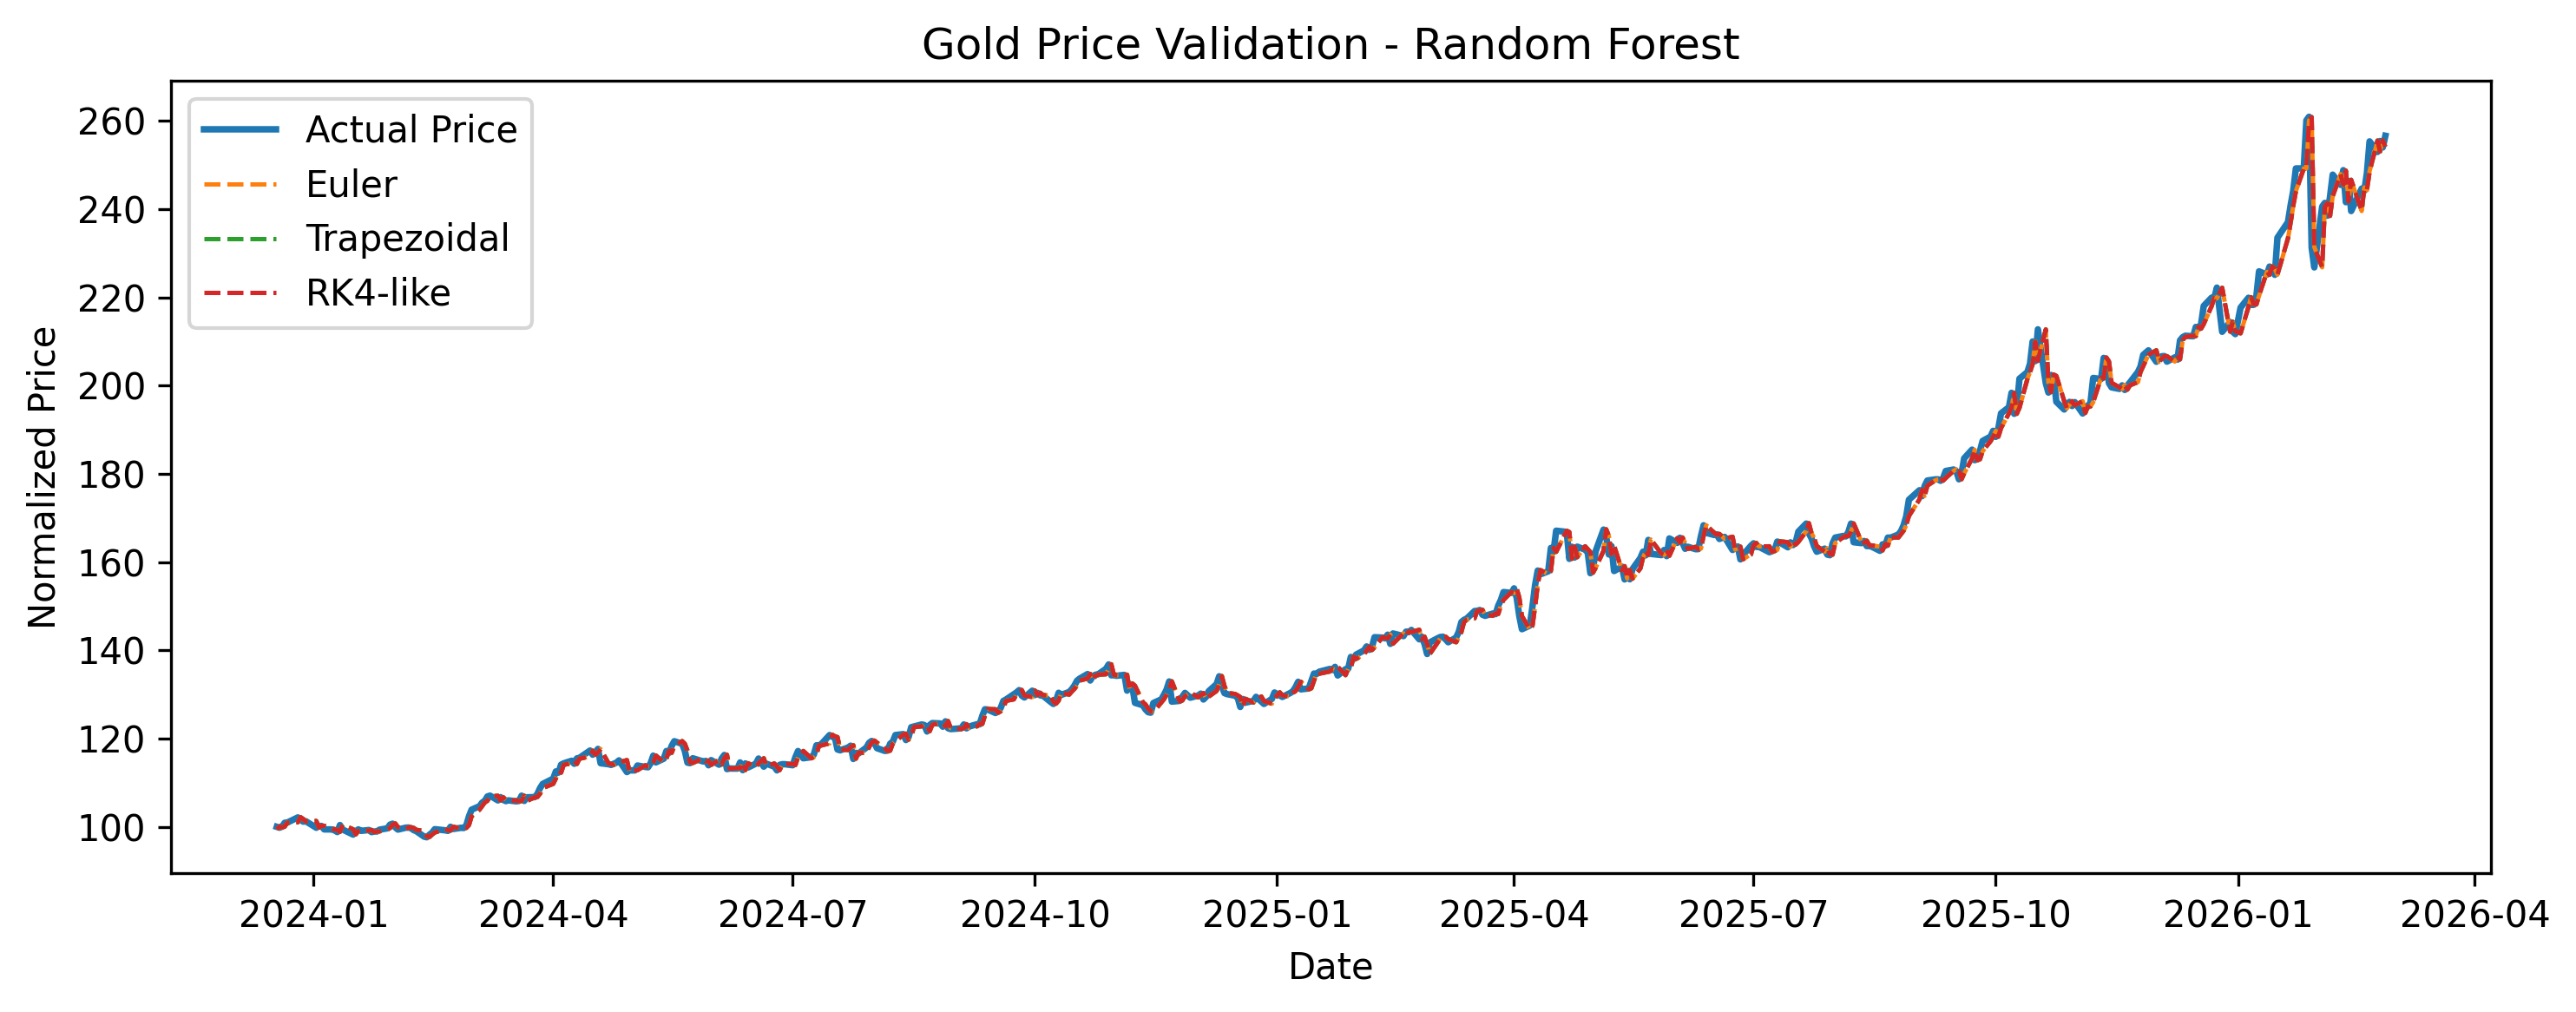
\includegraphics[width=\textwidth]{numerical_validation_plot/Gold_Random_Forest_price_validation.png}
        \caption{Gold -- RF}
    \end{subfigure}
    \hfill
    \begin{subfigure}[t]{0.31\textwidth}
        \centering
        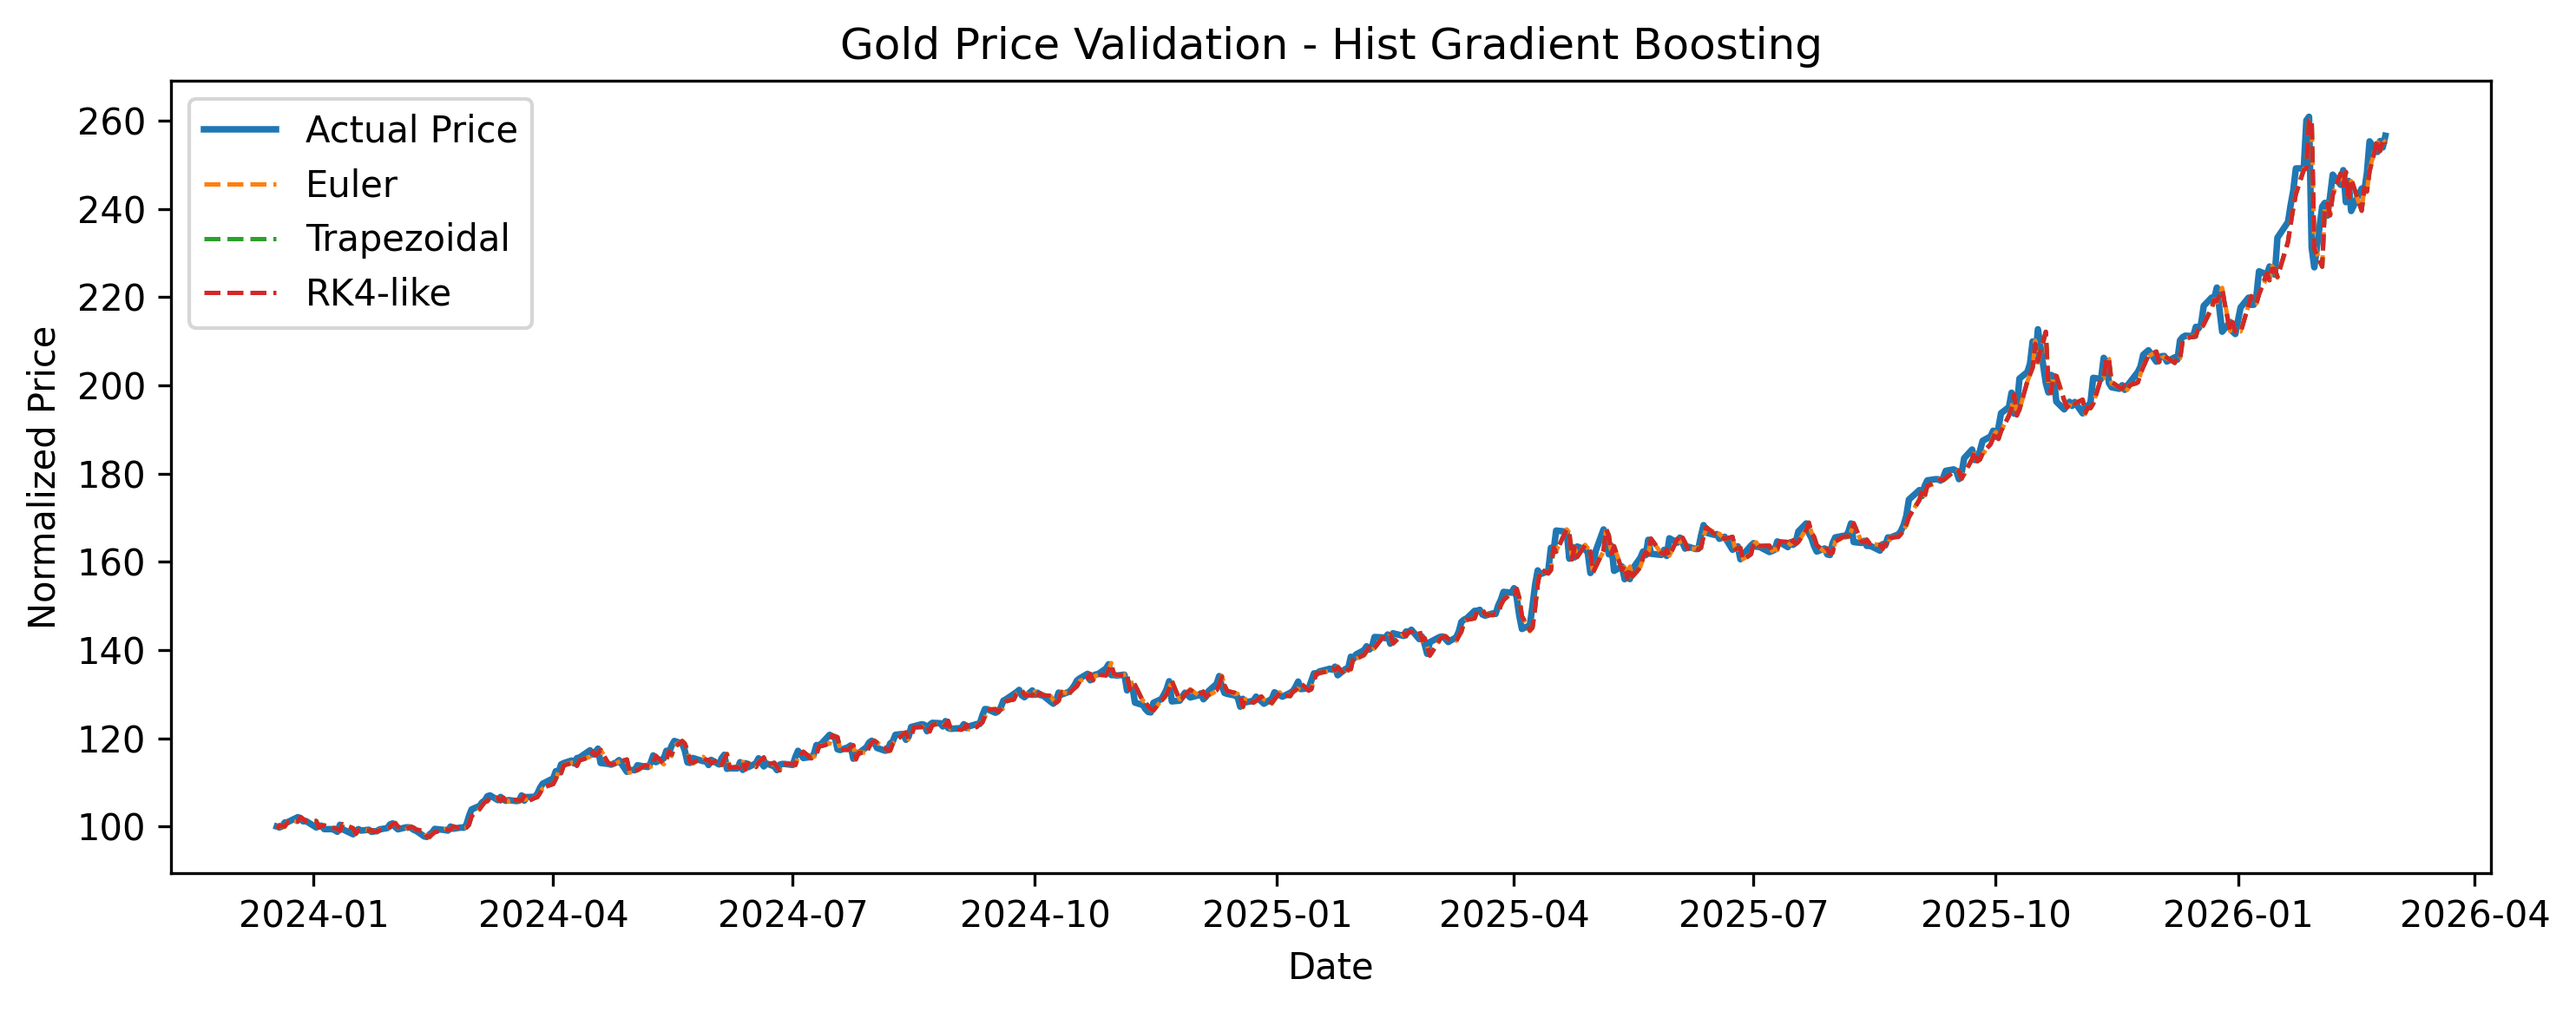
\includegraphics[width=\textwidth]{numerical_validation_plot/Gold_Hist_Gradient_Boosting_price_validation.png}
        \caption{Gold -- HGB}
    \end{subfigure}

    \vspace{0.15cm}

    % ---------------- Silver ----------------
    \begin{subfigure}[t]{0.31\textwidth}
        \centering
        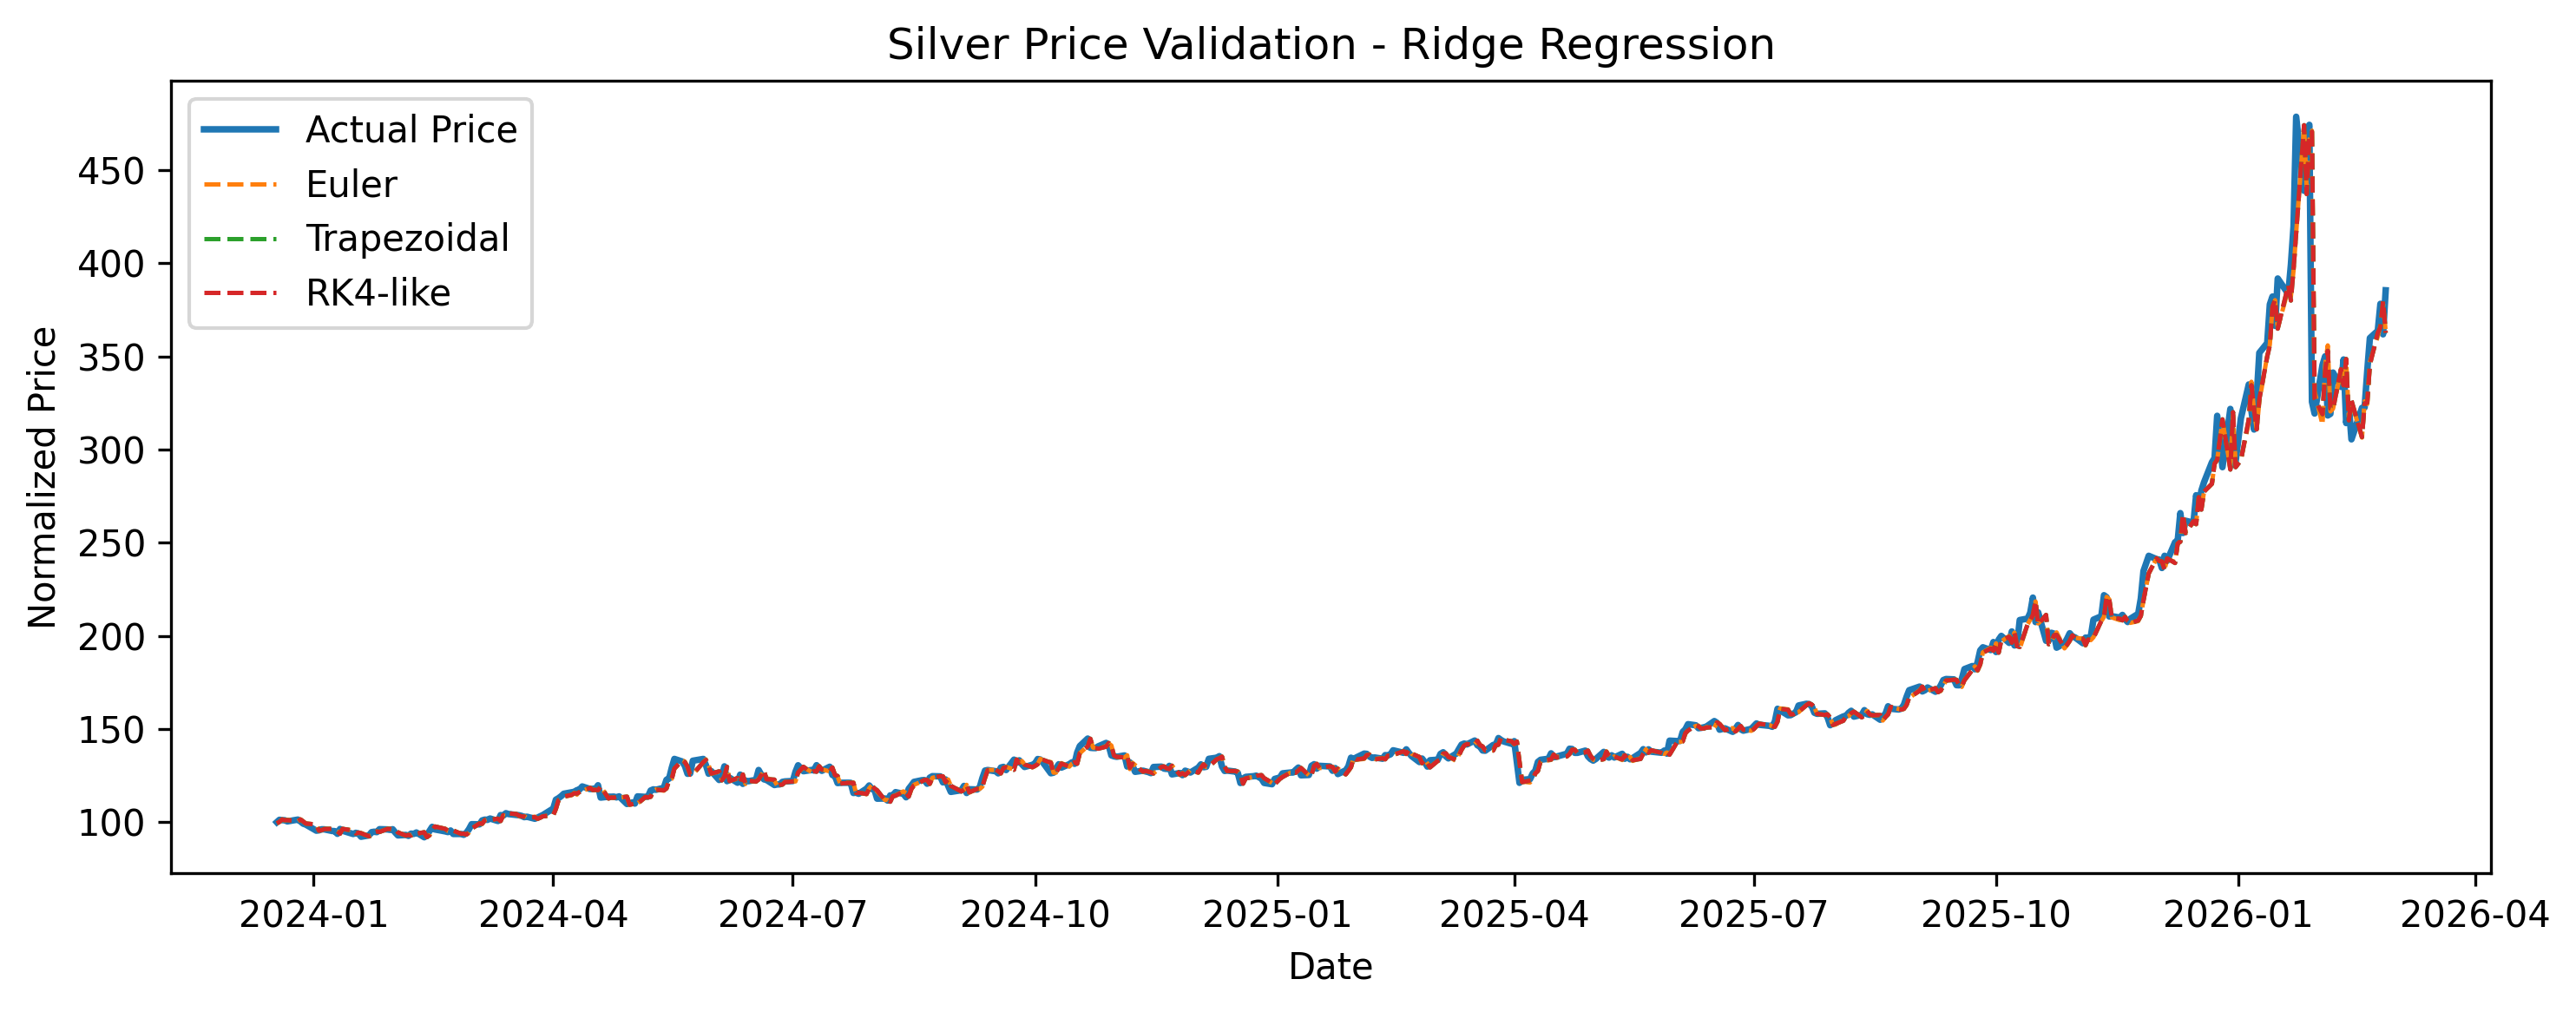
\includegraphics[width=\textwidth]{numerical_validation_plot/Silver_Ridge_Regression_price_validation.png}
        \caption{Silver -- Ridge}
    \end{subfigure}
    \hfill
    \begin{subfigure}[t]{0.31\textwidth}
        \centering
        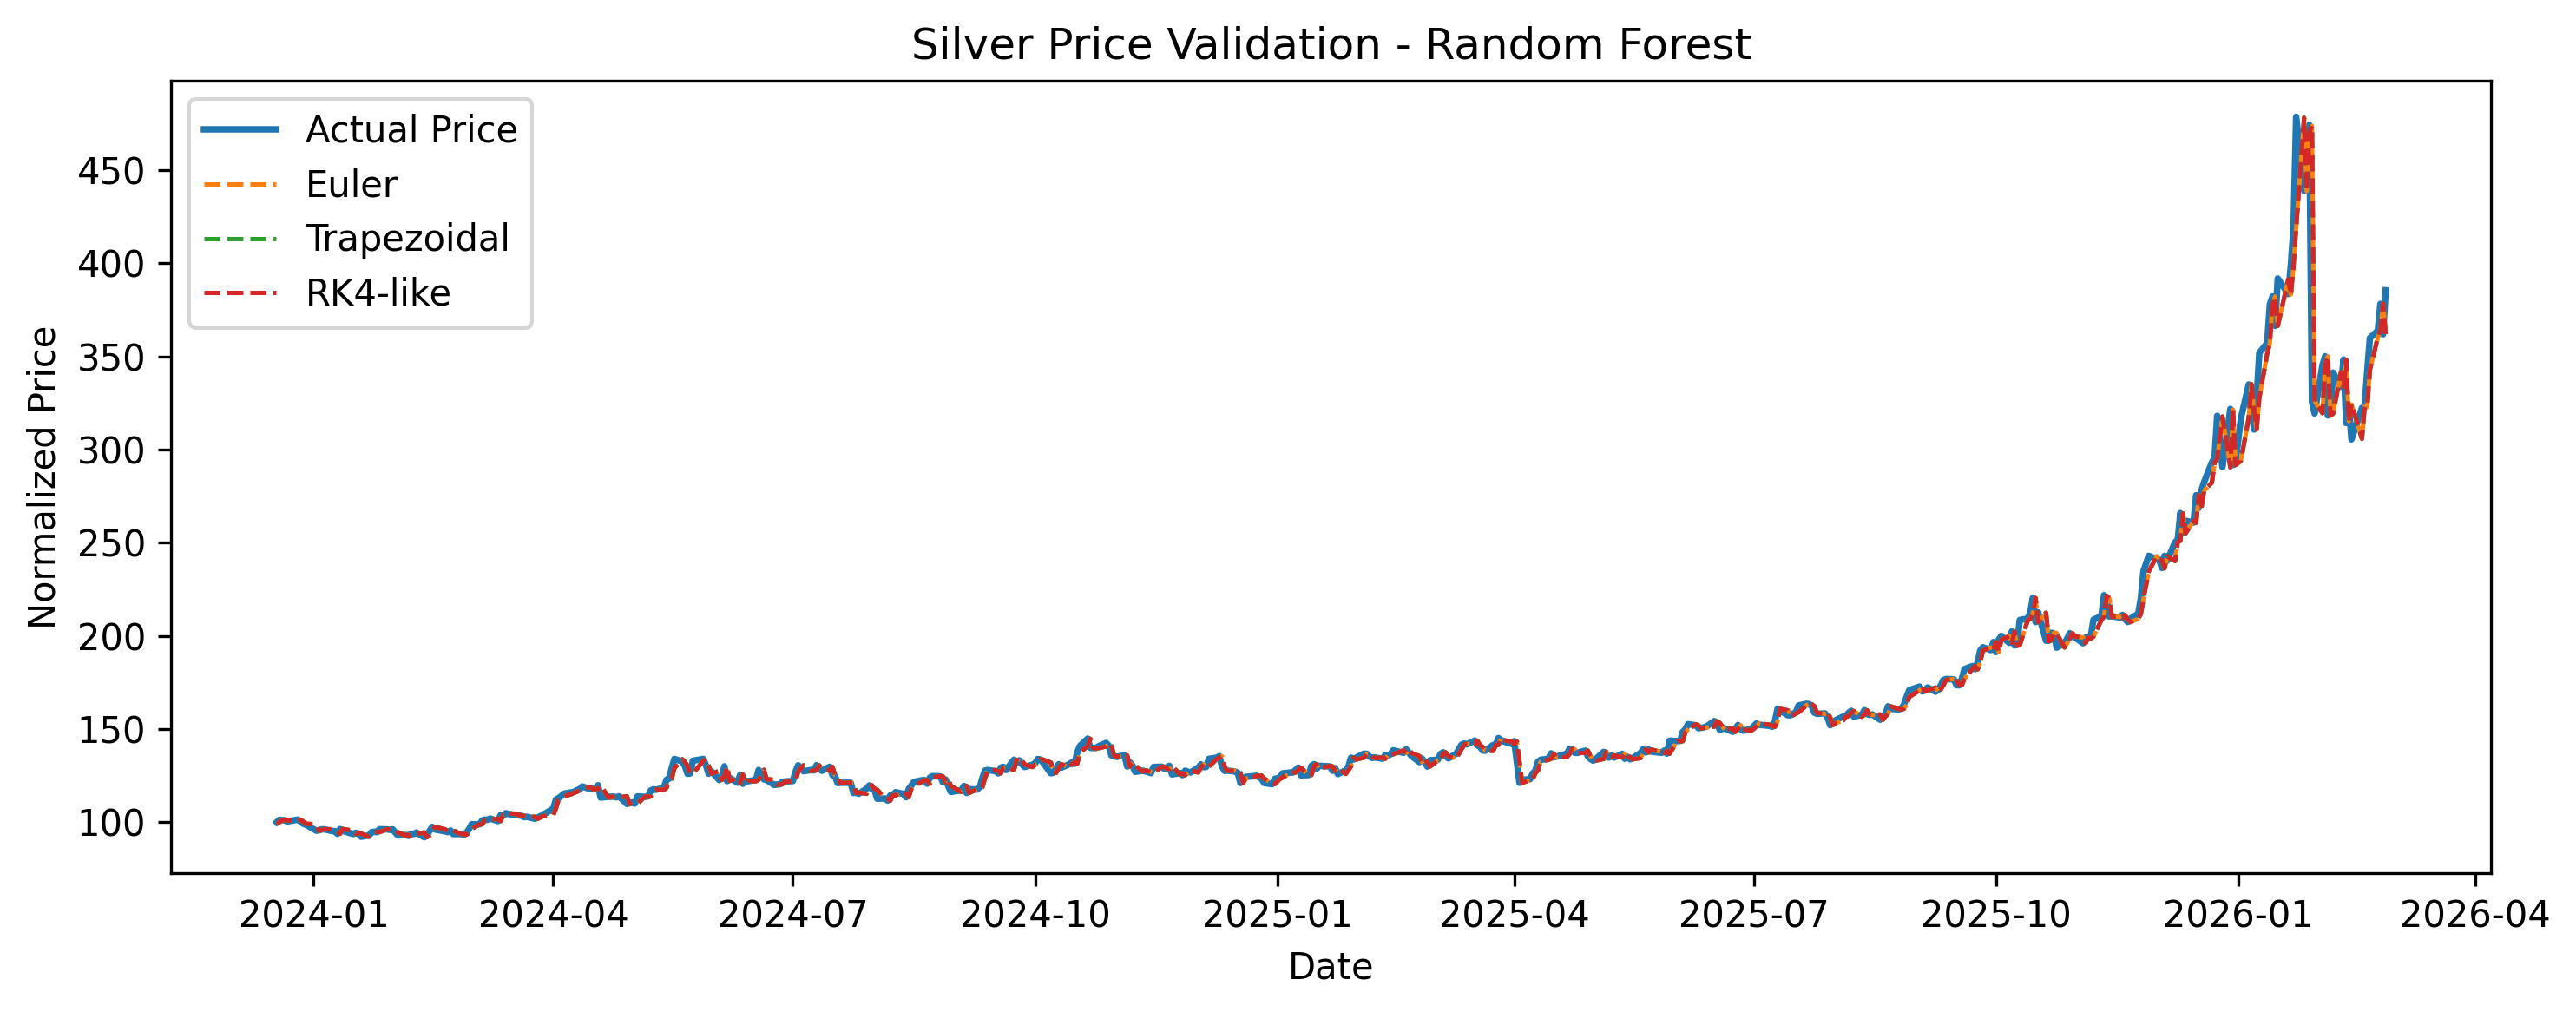
\includegraphics[width=\textwidth]{numerical_validation_plot/Silver_Random_Forest_price_validation.png}
        \caption{Silver -- RF}
    \end{subfigure}
    \hfill
    \begin{subfigure}[t]{0.31\textwidth}
        \centering
        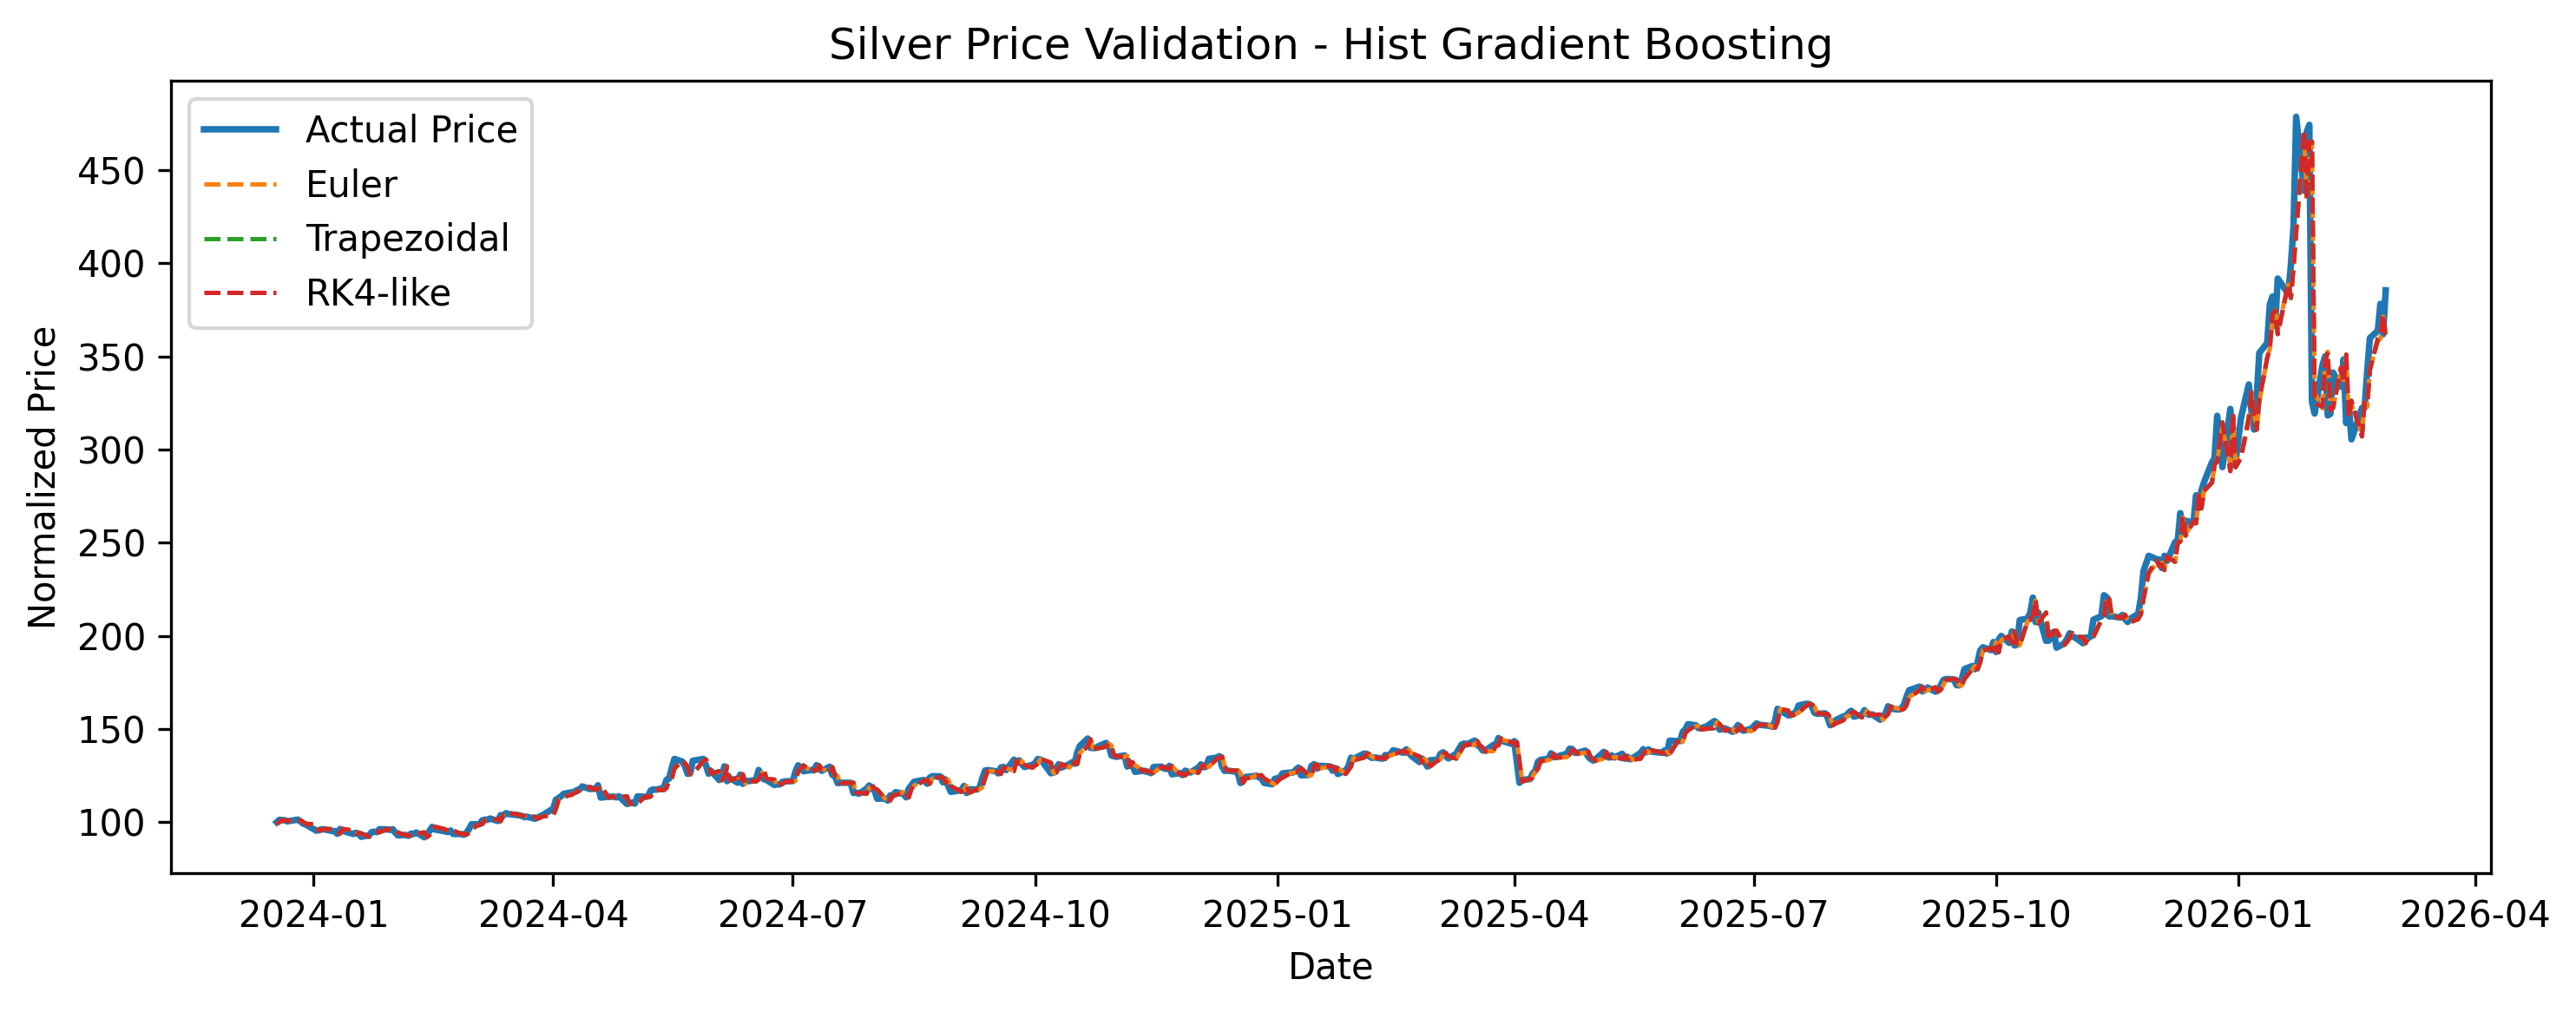
\includegraphics[width=\textwidth]{numerical_validation_plot/Silver_Hist_Gradient_Boosting_price_validation.png}
        \caption{Silver -- HGB}
    \end{subfigure}

    \caption{Actual vs Numerically Validated Predicted Prices for Gold and Silver}
    \label{fig:numerical_validation_metals}
\end{figure}

% ------------------------------------------------------------
% Figure: USD Index and WTI Oil
% ------------------------------------------------------------

\begin{figure}[H]
    \centering
    \captionsetup[subfigure]{skip=4pt}
    
    % ---------------- USD Index ----------------
    \begin{subfigure}[t]{0.31\textwidth}
        \centering
        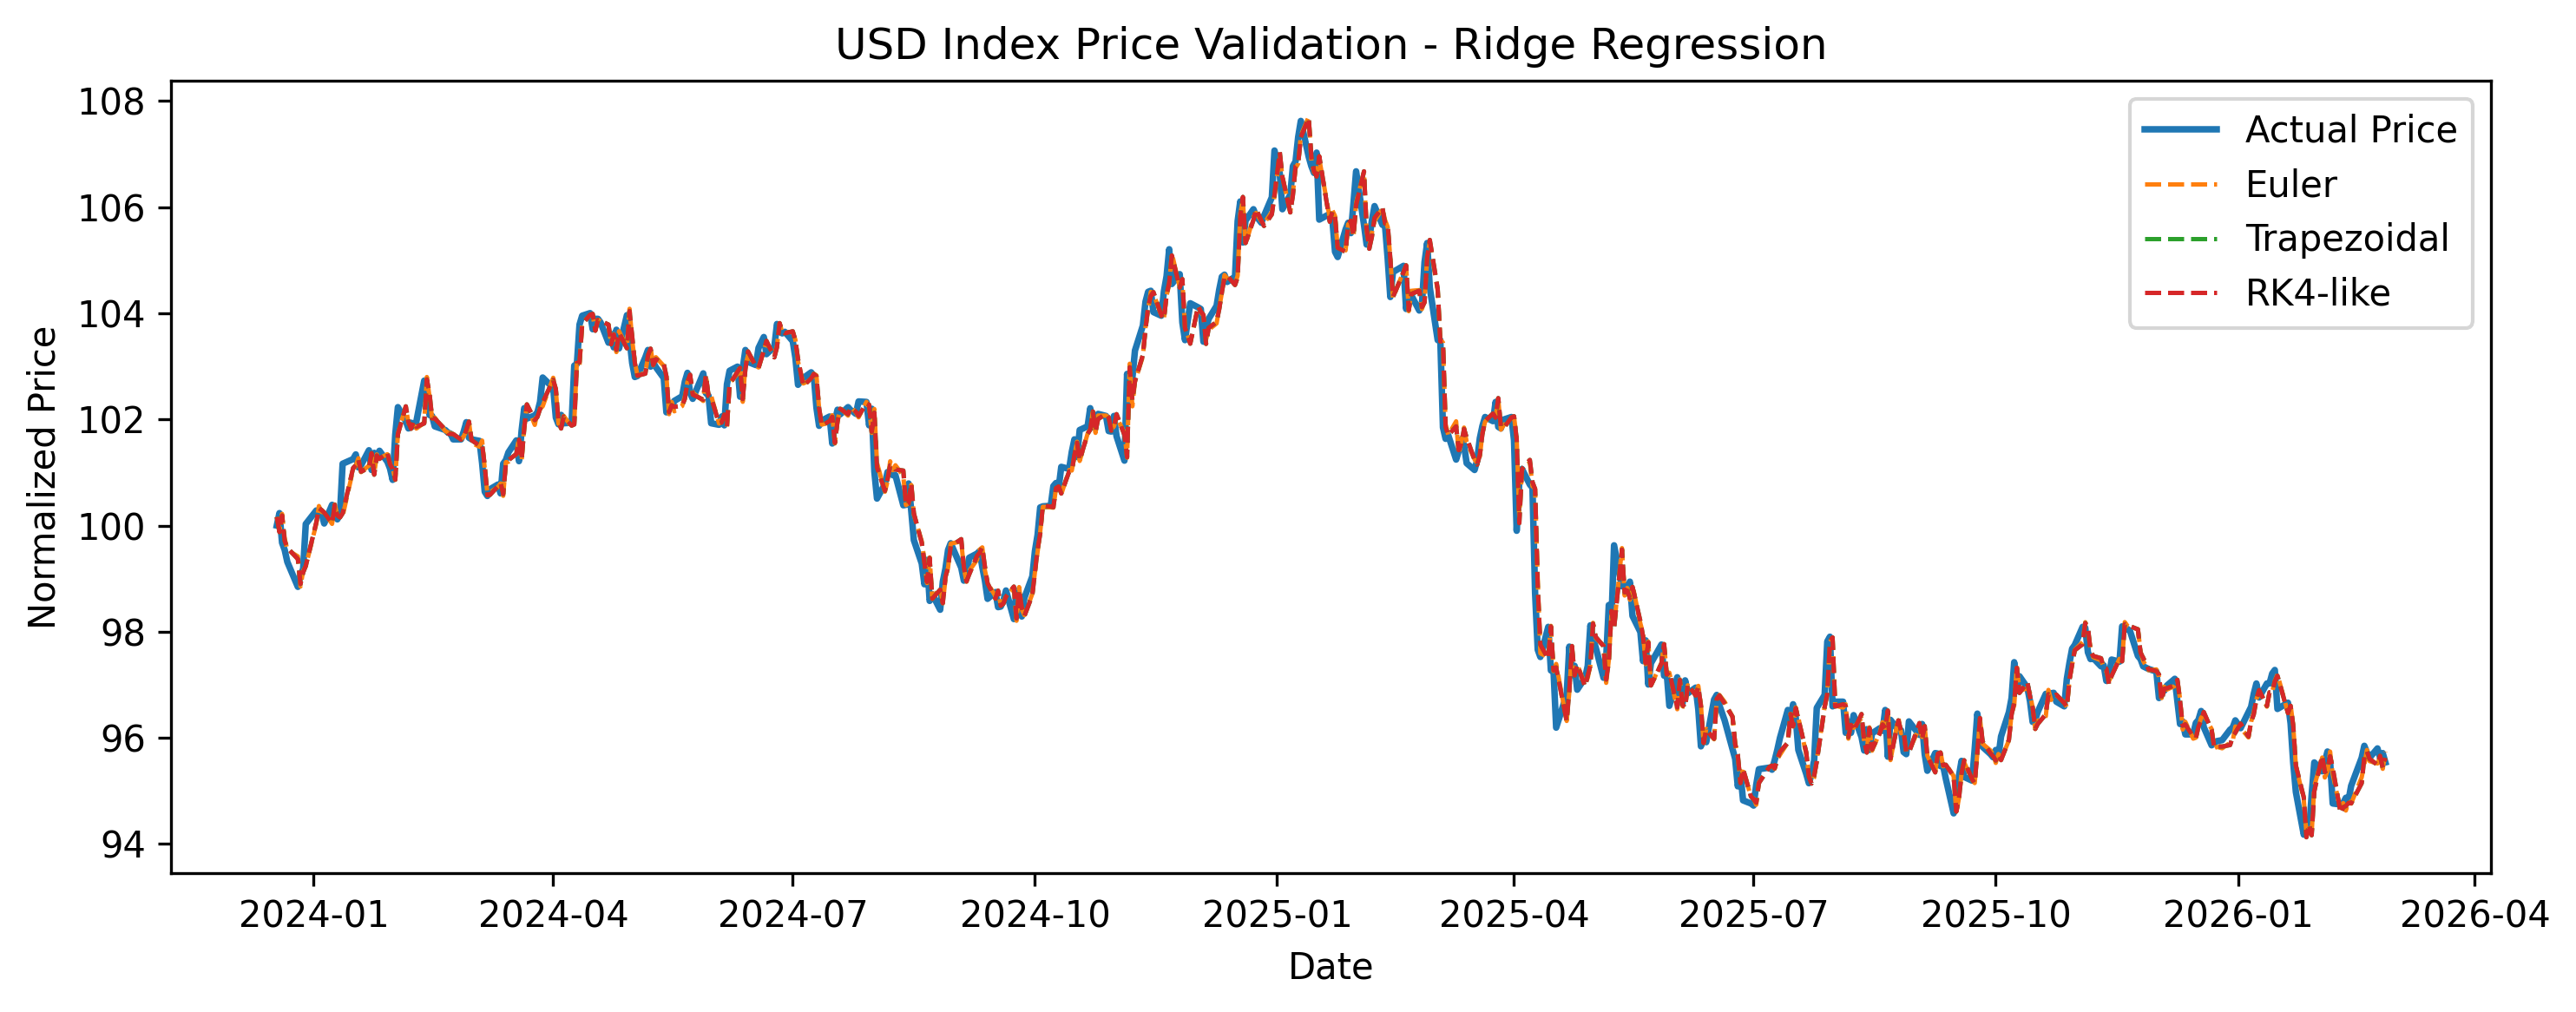
\includegraphics[width=\textwidth]{numerical_validation_plot/USD_Index_Ridge_Regression_price_validation.png}
        \caption{USD Index -- Ridge}
    \end{subfigure}
    \hfill
    \begin{subfigure}[t]{0.31\textwidth}
        \centering
        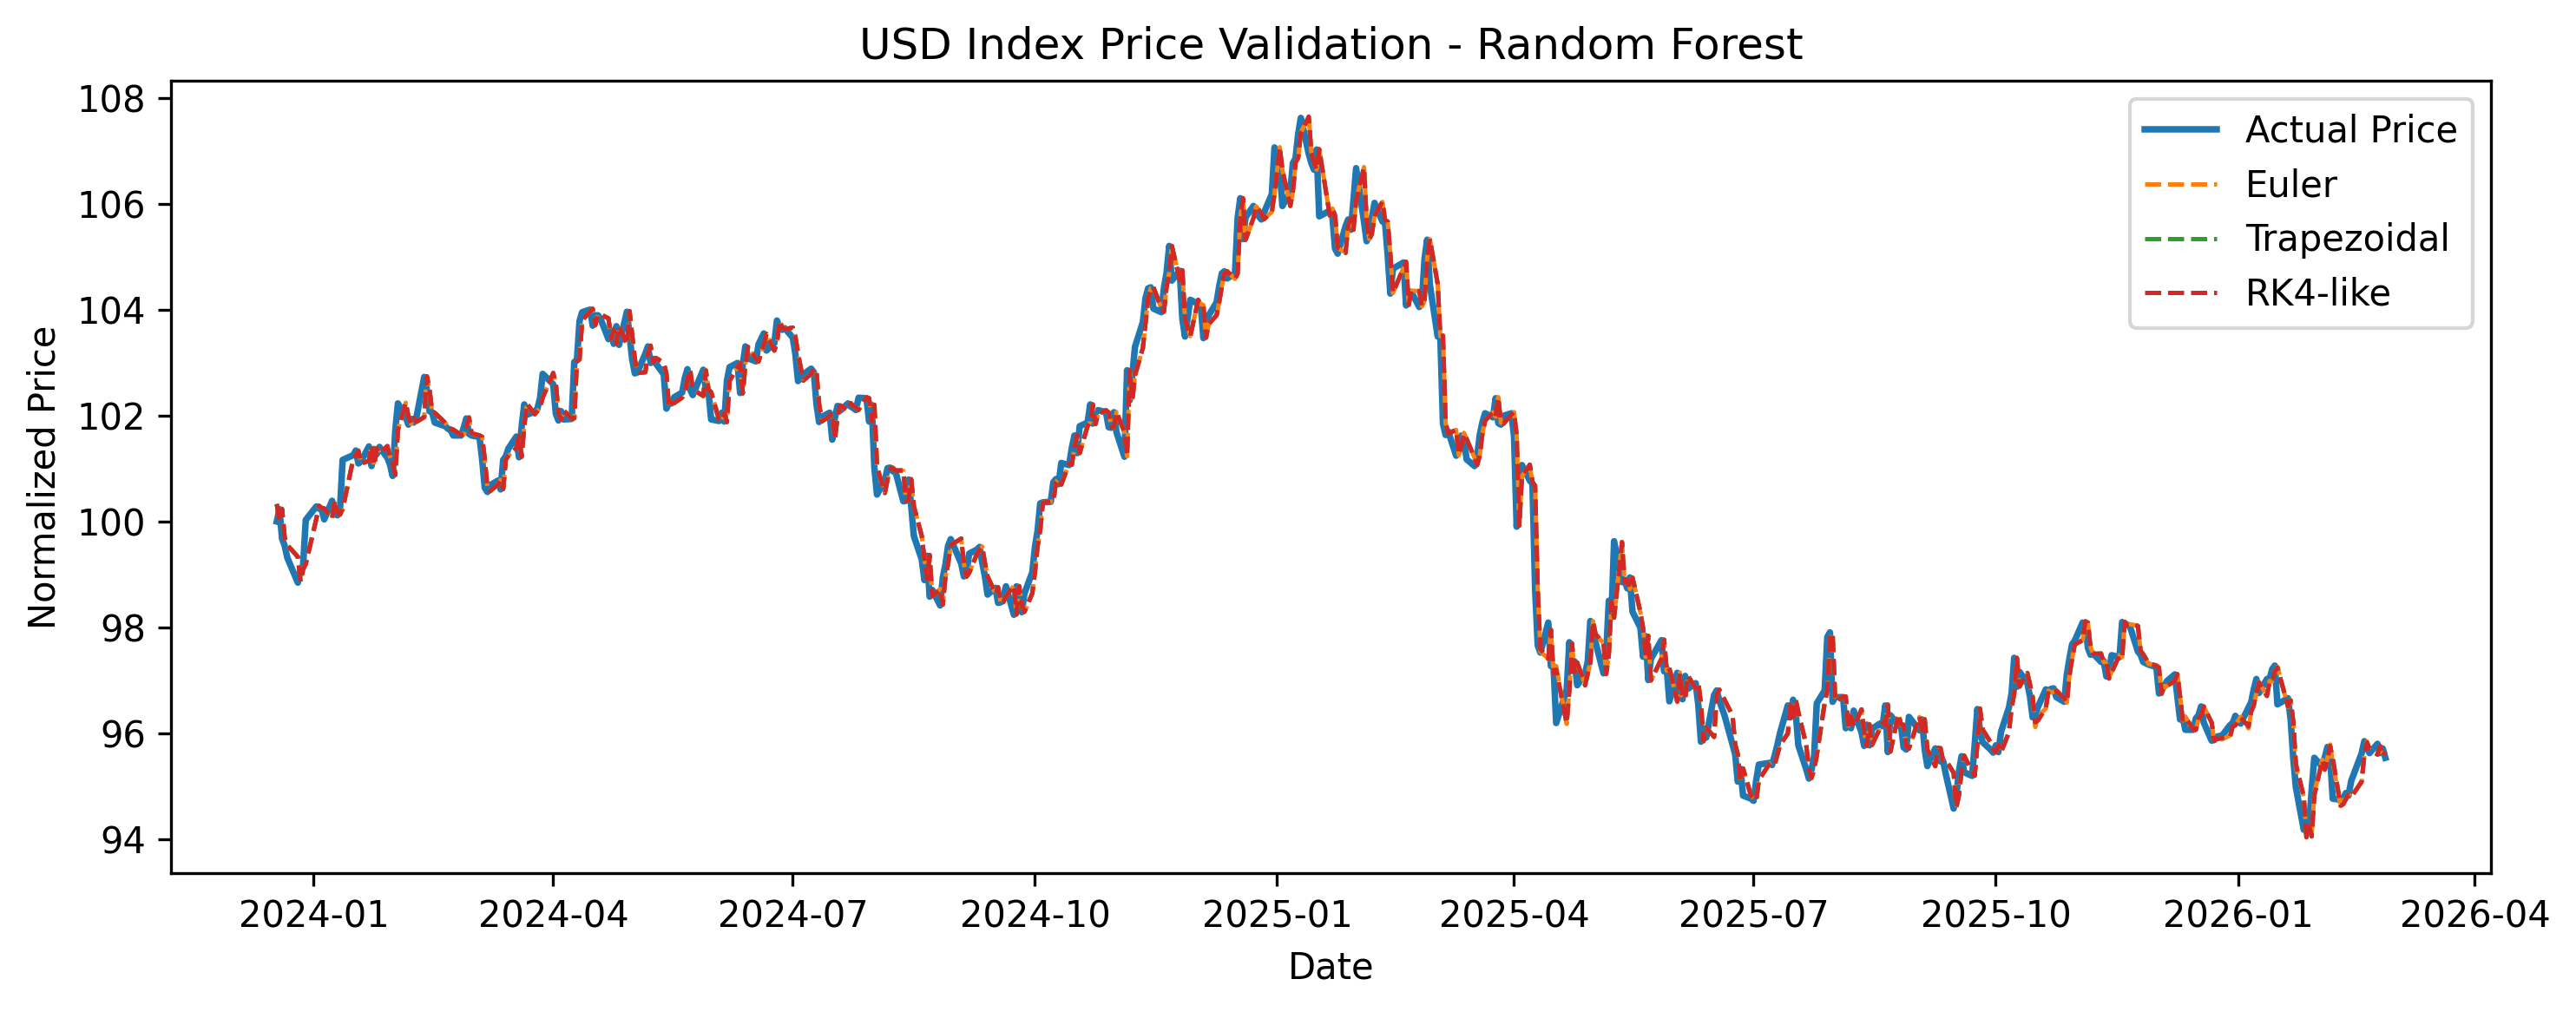
\includegraphics[width=\textwidth]{numerical_validation_plot/USD_Index_Random_Forest_price_validation.png}
        \caption{USD Index -- RF}
    \end{subfigure}
    \hfill
    \begin{subfigure}[t]{0.31\textwidth}
        \centering
        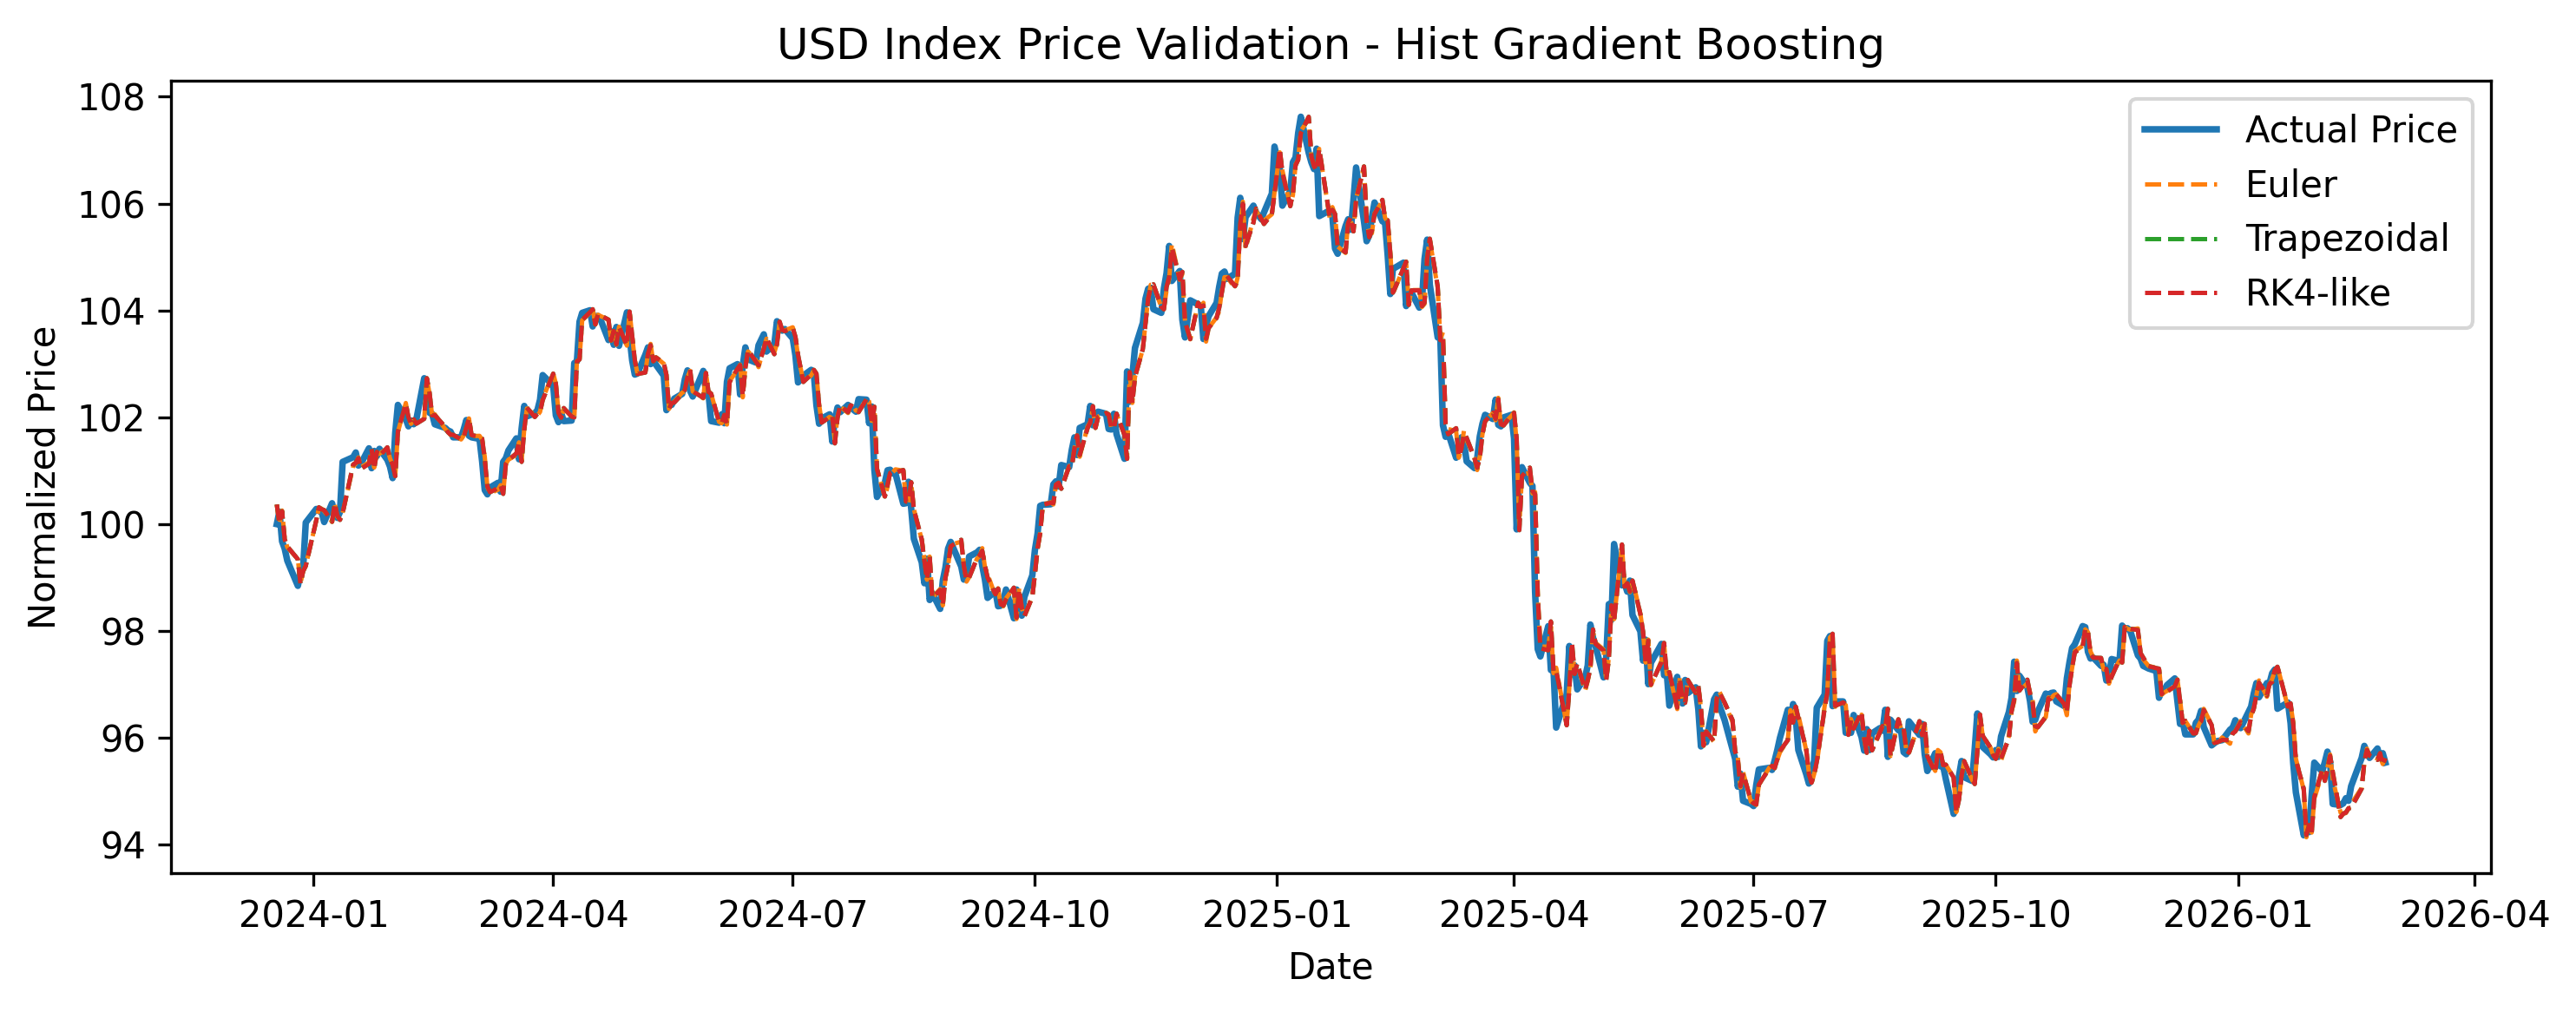
\includegraphics[width=\textwidth]{numerical_validation_plot/USD_Index_Hist_Gradient_Boosting_price_validation.png}
        \caption{USD Index -- HGB}
    \end{subfigure}

    \vspace{0.15cm}

    % ---------------- WTI Oil ----------------
    \begin{subfigure}[t]{0.31\textwidth}
        \centering
        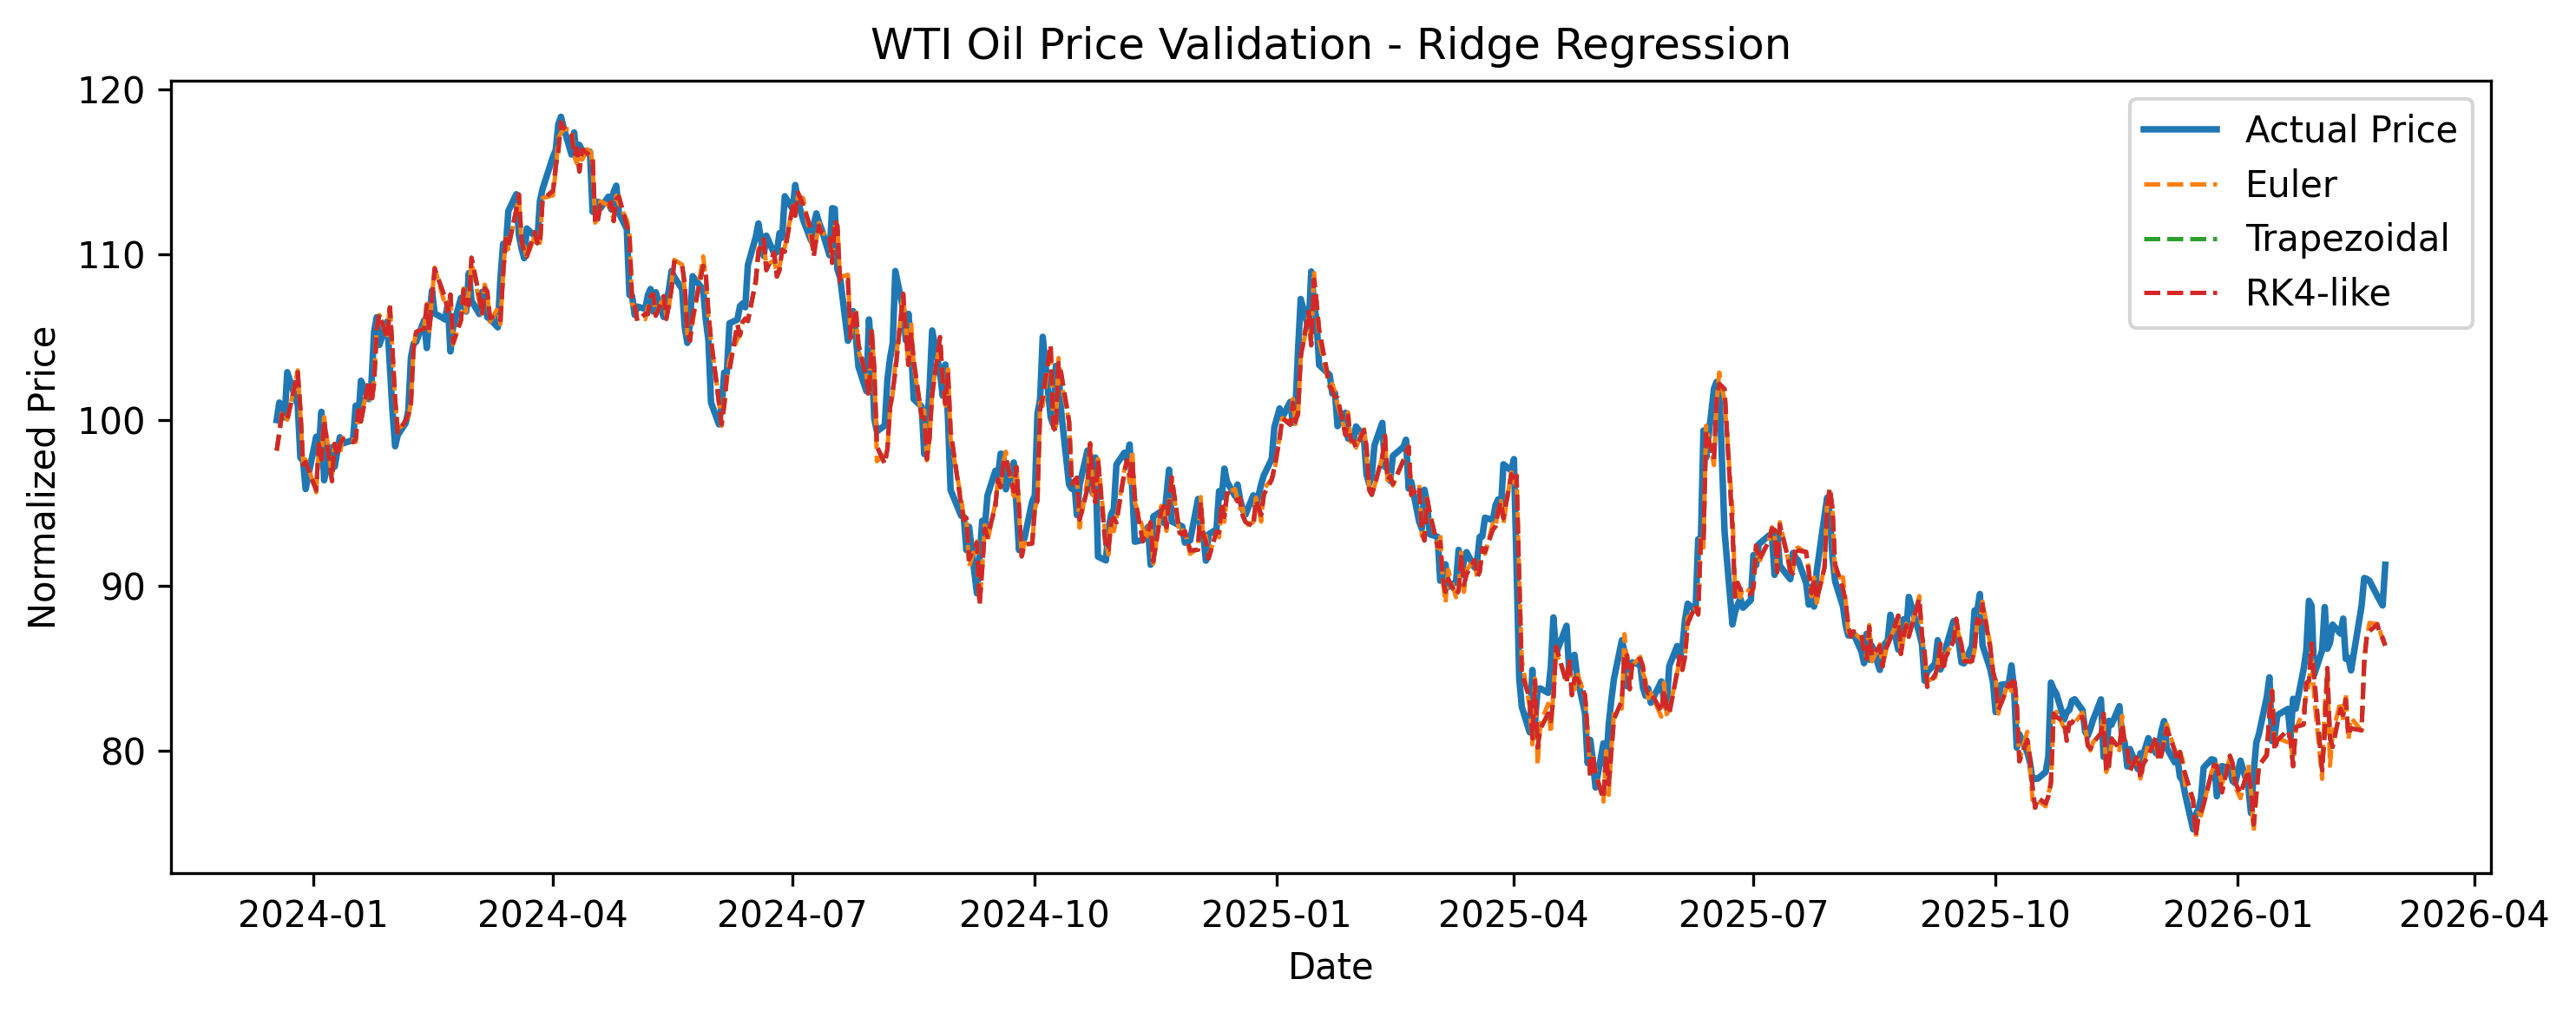
\includegraphics[width=\textwidth]{numerical_validation_plot/WTI_Oil_Ridge_Regression_price_validation.png}
        \caption{WTI Oil -- Ridge}
    \end{subfigure}
    \hfill
    \begin{subfigure}[t]{0.31\textwidth}
        \centering
        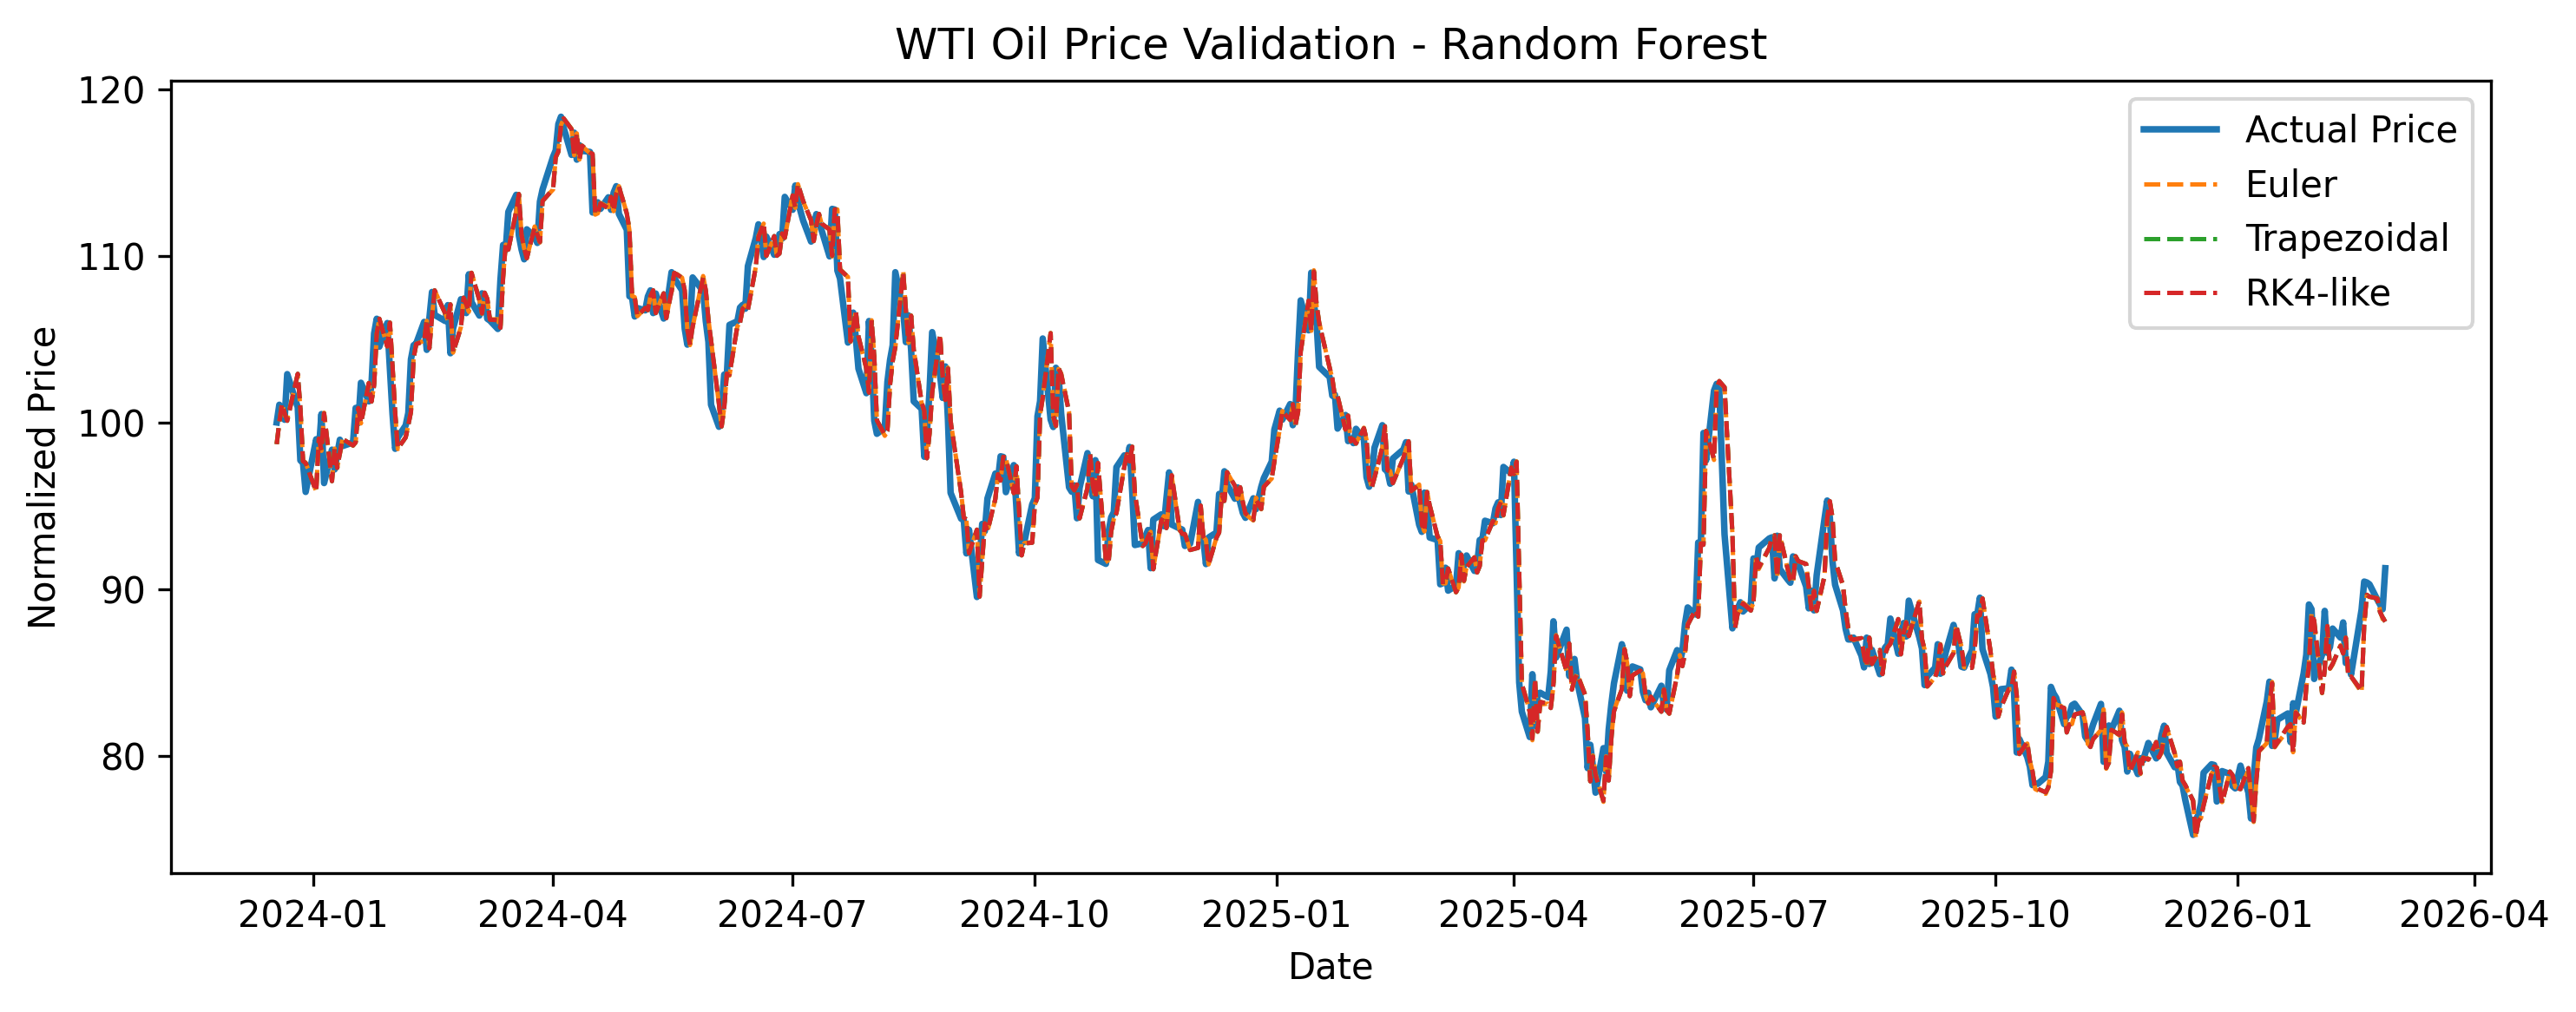
\includegraphics[width=\textwidth]{numerical_validation_plot/WTI_Oil_Random_Forest_price_validation.png}
        \caption{WTI Oil -- RF}
    \end{subfigure}
    \hfill
    \begin{subfigure}[t]{0.31\textwidth}
        \centering
        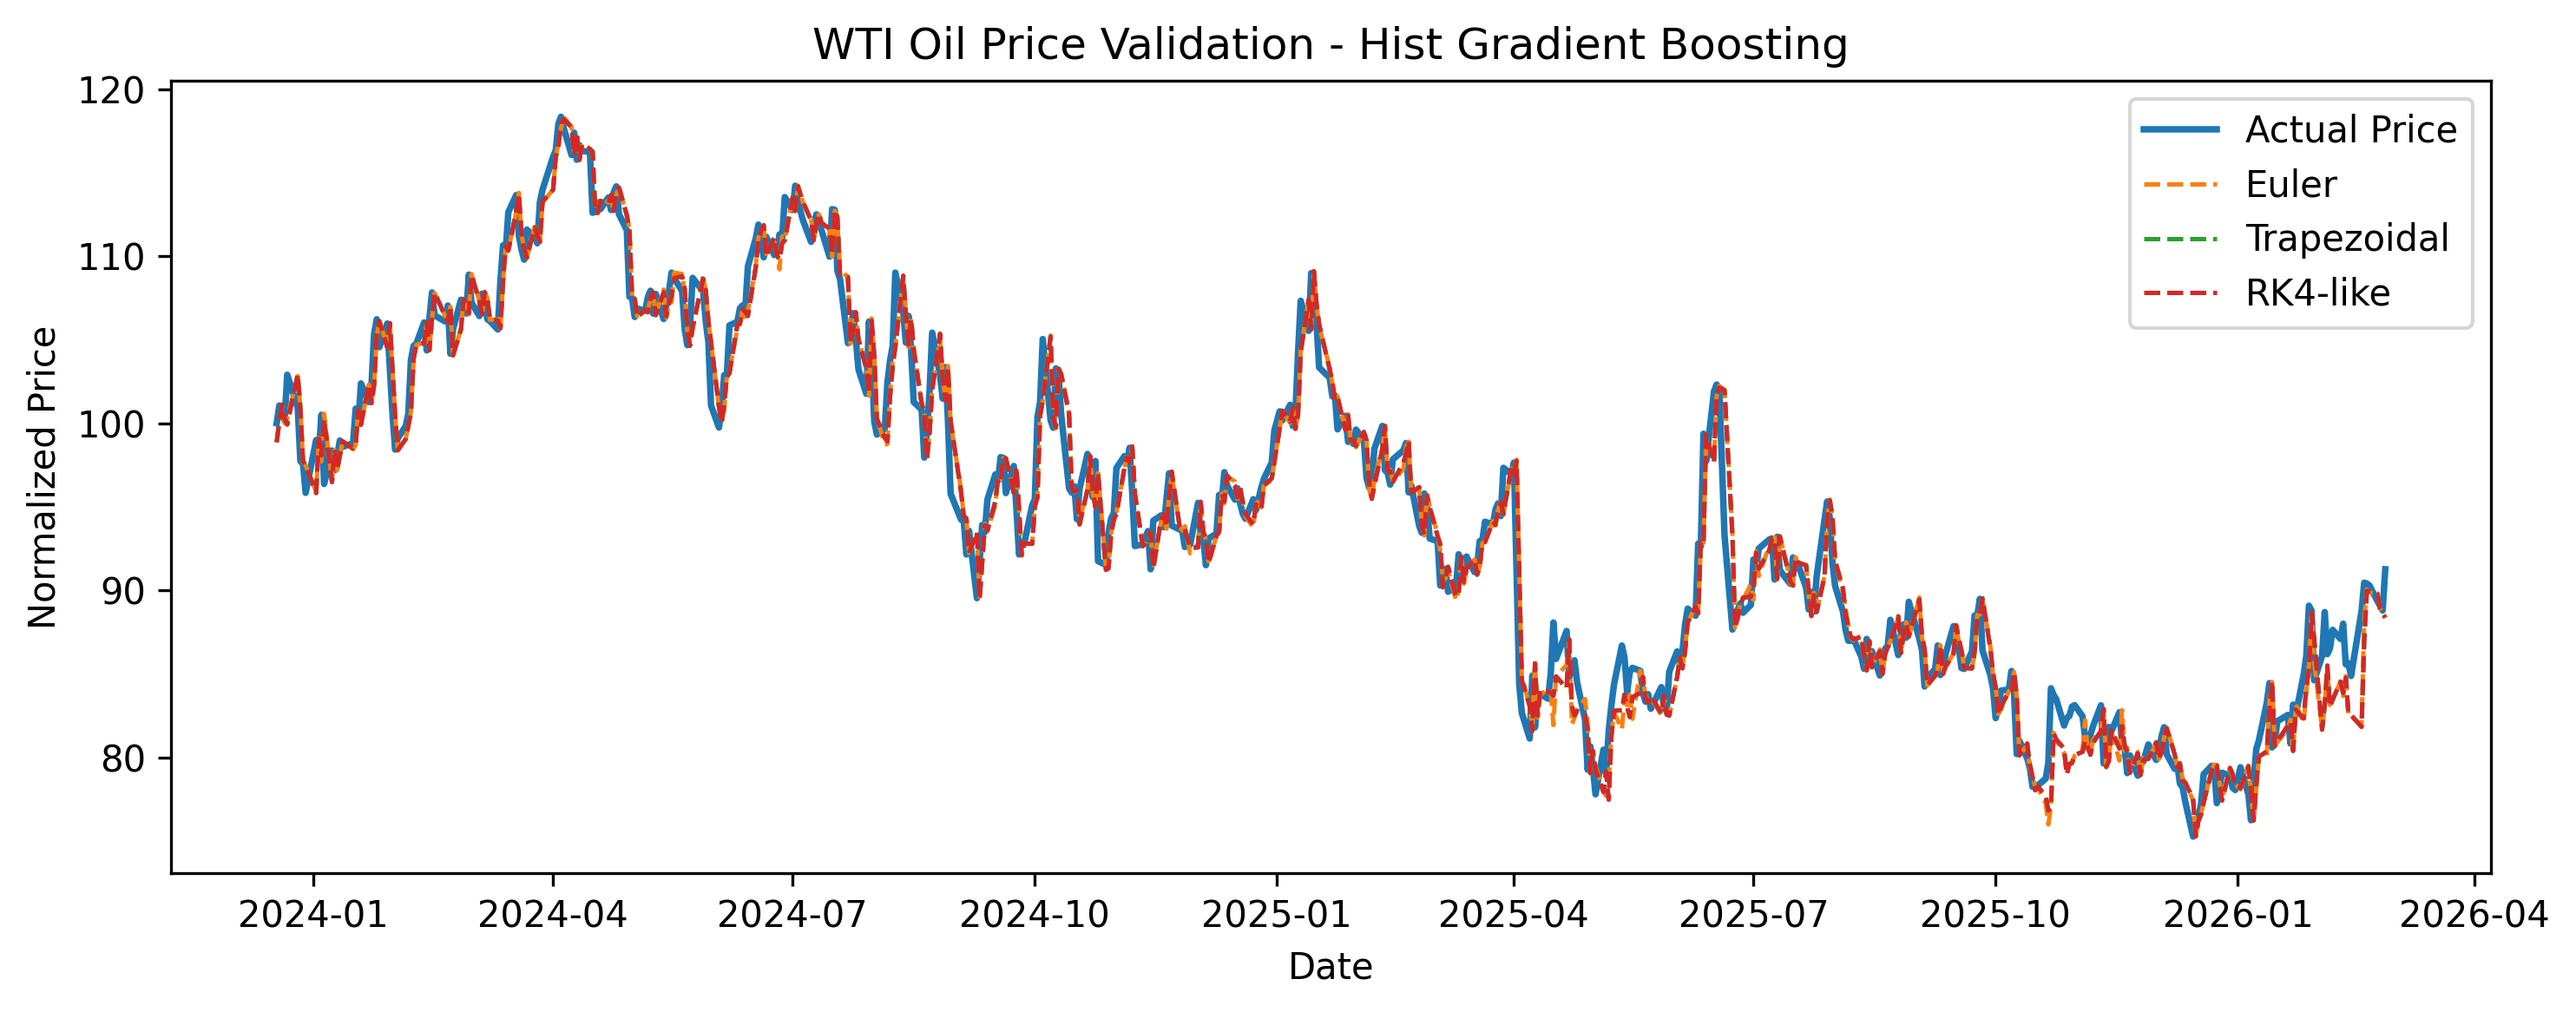
\includegraphics[width=\textwidth]{numerical_validation_plot/WTI_Oil_Hist_Gradient_Boosting_price_validation.png}
        \caption{WTI Oil -- HGB}
    \end{subfigure}

    \caption{Actual vs Numerically Validated Predicted Prices for USD Index and WTI Oil}
    \label{fig:numerical_validation_macro}
\end{figure}

\subsection{Discussion}

Overall, the numerical validation results support the conclusions from the supervised learning analysis. Random Forest remains the strongest overall predictive model for most assets, while Hist Gradient Boosting performs especially well for Silver. After converting predicted next-day returns into predicted price paths, the Euler method most frequently produces the lowest prediction error, making it the most reliable numerical updating rule in this project.

This result is reasonable because the supervised learning models directly predict discrete daily log returns rather than continuous-time derivatives. Therefore, the numerical validation step mainly evaluates how well these predicted returns can reconstruct realistic price trajectories. Under this setting, the simple Euler update is often sufficient because it directly applies the one-step predicted return to the current price. More complex methods such as the Trapezoidal and RK4-like approaches introduce additional smoothing or weighted averaging, but they do not consistently improve accuracy.

The results are also consistent with the earlier EDA findings. Assets with smoother price behavior, such as Gold and the USD Index, tend to have smaller validation errors, while highly volatile assets such as Bitcoin and Ethereum are more difficult to predict accurately. Overall, the numerical validation confirms that the supervised learning framework is stable and that the predicted return signals can produce reasonable price paths across different asset classes.

% ============================================================
% Web Application
% ============================================================

\section{Interactive Web Application}

To make the project results easier to explore, we also developed an interactive Shiny web application. The web application summarizes the main components of the project, including data cleaning, exploratory data analysis, feature engineering, unsupervised learning, supervised machine learning models, and numerical method validation.

The application allows users to interactively select different assets and models, view prediction plots, compare model performance tables, and examine numerical validation results. Compared with the static report, the web application provides a more flexible way to explore the results and better understand how the prediction framework performs across different financial assets.

The deployed Shiny application is available at:

\begin{center}
\href{https://baixuanchen5243.shinyapps.io/5291-Final-Project/}
{https://baixuanchen5243.shinyapps.io/5291-Final-Project/}
\end{center}

Overall, the web application serves as an interactive supplement to the written report and helps present the complete financial time series prediction workflow in a clear and user-friendly format.

% ============================================================
% 9. Results and Discussion
% ============================================================

% ============================================================
% 9. Results and Discussion
% ============================================================

\section{Results and Discussion}

The results show that financial time series prediction is difficult because asset returns are noisy, nonlinear, and strongly affected by changing market conditions. Although the supervised learning models were able to capture some useful patterns from the engineered features, the prediction performance varied across assets. Relatively stable assets such as Gold and the USD Index were easier to model, while Bitcoin, Ethereum, and WTI Oil were more difficult because of higher volatility and more extreme price movements.

\subsection{Challenges}

One major challenge was the noisy nature of short-horizon return prediction. Since the target variable was the next-day log return, the models had to predict very small and highly random daily movements. This explains why some $R^2$ values were low or negative, even when the predicted price paths visually followed the broad market trend.

Another challenge was avoiding data leakage. Because this is a time series problem, the training and testing sets had to be split chronologically. In addition, lagged features, rolling statistics, target construction, and price reconstruction needed to be carefully aligned so that future information was not accidentally used during model training.

A third challenge was model interpretation. Random Forest and Hist Gradient Boosting generally performed better than Ridge Regression, but tree-based ensemble models are less transparent than linear models. Therefore, the final comparison relied on multiple forms of evidence, including RMSE, MAE, directional accuracy, return prediction plots, price prediction plots, and numerical validation results.

\subsection{Future Work}

Future work could improve the project in several directions. First, more advanced time series models, such as LSTM, GRU, or Transformer-based models, could be tested to capture longer-term temporal dependence in financial data. These models may be useful for assets with strong nonlinear dynamics and volatility clustering.

Second, additional explanatory variables could be added, such as trading volume, interest rates, macroeconomic indicators, market sentiment, or volatility indices. These variables may provide information beyond historical prices and returns.

Third, the validation framework could be extended by using rolling-window or expanding-window backtesting instead of only one chronological train-test split. This would make the evaluation more robust across different market regimes.

Finally, the Shiny application could be further improved by adding downloadable prediction outputs, additional interactive filters, user-selected time windows, and more detailed model comparison tools. This would make the application more useful as an exploratory platform for financial time series analysis.


% ============================================================
% 10. Conclusion
% ============================================================

\section{Conclusion}

This project developed a financial time series prediction framework for six assets: Gold, Silver, WTI Oil, USD Index, Bitcoin, and Ethereum. The workflow included data cleaning, exploratory data analysis, feature engineering, unsupervised learning, supervised machine learning, numerical method validation, and an interactive Shiny web application.

The exploratory analysis showed clear differences among the six assets. Cryptocurrencies had higher volatility and more extreme return behavior, while Gold and the USD Index were relatively more stable. These findings supported the construction of extended financial features, including lagged returns, rolling volatility, momentum, volatility ratios, rolling correlations, drawdowns, and extreme-return indicators.

The unsupervised analysis provided additional insight into market structure. PCA reduced the high-dimensional feature space, K-Means clustering helped identify different market condition groups, and Isolation Forest detected unusual market observations. These results showed that market behavior changes over time and that volatility regimes and extreme events are important for financial prediction.

For supervised learning, Ridge Regression, Random Forest, and Hist Gradient Boosting were compared. Overall, the nonlinear tree-based models performed better than the linear Ridge Regression benchmark. Random Forest was the strongest overall model, achieving the best RMSE for most assets, while Hist Gradient Boosting performed best for Silver. The return prediction plots showed the direct model forecasts, and the price prediction plots helped explain how predicted returns translated into reconstructed price paths.

The numerical method validation showed that the Euler method was the most reliable overall approach for converting predicted next-day returns into predicted price paths. This result is reasonable because the supervised models predicted discrete daily returns rather than continuous-time derivatives, so a simple one-step updating rule was sufficient.

In conclusion, this project shows that combining careful feature engineering, nonlinear machine learning models, and numerical validation can provide a useful framework for financial time series prediction. Although short-term financial returns remain difficult to forecast, Random Forest with engineered financial features and Euler-based price reconstruction provided the most stable overall approach in this project. The Shiny web application further improves the presentation of the project by allowing users to interactively explore the data, models, prediction plots, and validation results.

\end{document}